% Options for packages loaded elsewhere
\PassOptionsToPackage{unicode}{hyperref}
\PassOptionsToPackage{hyphens}{url}
%
\documentclass[
  letterpaper,
]{book}

\usepackage{amsmath,amssymb}
\usepackage{iftex}
\ifPDFTeX
  \usepackage[T1]{fontenc}
  \usepackage[utf8]{inputenc}
  \usepackage{textcomp} % provide euro and other symbols
\else % if luatex or xetex
  \usepackage{unicode-math}
  \defaultfontfeatures{Scale=MatchLowercase}
  \defaultfontfeatures[\rmfamily]{Ligatures=TeX,Scale=1}
\fi
\usepackage{lmodern}
\ifPDFTeX\else  
    % xetex/luatex font selection
\fi
% Use upquote if available, for straight quotes in verbatim environments
\IfFileExists{upquote.sty}{\usepackage{upquote}}{}
\IfFileExists{microtype.sty}{% use microtype if available
  \usepackage[]{microtype}
  \UseMicrotypeSet[protrusion]{basicmath} % disable protrusion for tt fonts
}{}
\makeatletter
\@ifundefined{KOMAClassName}{% if non-KOMA class
  \IfFileExists{parskip.sty}{%
    \usepackage{parskip}
  }{% else
    \setlength{\parindent}{0pt}
    \setlength{\parskip}{6pt plus 2pt minus 1pt}}
}{% if KOMA class
  \KOMAoptions{parskip=half}}
\makeatother
\usepackage{xcolor}
\setlength{\emergencystretch}{3em} % prevent overfull lines
\setcounter{secnumdepth}{5}
% Make \paragraph and \subparagraph free-standing
\makeatletter
\ifx\paragraph\undefined\else
  \let\oldparagraph\paragraph
  \renewcommand{\paragraph}{
    \@ifstar
      \xxxParagraphStar
      \xxxParagraphNoStar
  }
  \newcommand{\xxxParagraphStar}[1]{\oldparagraph*{#1}\mbox{}}
  \newcommand{\xxxParagraphNoStar}[1]{\oldparagraph{#1}\mbox{}}
\fi
\ifx\subparagraph\undefined\else
  \let\oldsubparagraph\subparagraph
  \renewcommand{\subparagraph}{
    \@ifstar
      \xxxSubParagraphStar
      \xxxSubParagraphNoStar
  }
  \newcommand{\xxxSubParagraphStar}[1]{\oldsubparagraph*{#1}\mbox{}}
  \newcommand{\xxxSubParagraphNoStar}[1]{\oldsubparagraph{#1}\mbox{}}
\fi
\makeatother


\providecommand{\tightlist}{%
  \setlength{\itemsep}{0pt}\setlength{\parskip}{0pt}}\usepackage{longtable,booktabs,array}
\usepackage{calc} % for calculating minipage widths
% Correct order of tables after \paragraph or \subparagraph
\usepackage{etoolbox}
\makeatletter
\patchcmd\longtable{\par}{\if@noskipsec\mbox{}\fi\par}{}{}
\makeatother
% Allow footnotes in longtable head/foot
\IfFileExists{footnotehyper.sty}{\usepackage{footnotehyper}}{\usepackage{footnote}}
\makesavenoteenv{longtable}
\usepackage{graphicx}
\makeatletter
\def\maxwidth{\ifdim\Gin@nat@width>\linewidth\linewidth\else\Gin@nat@width\fi}
\def\maxheight{\ifdim\Gin@nat@height>\textheight\textheight\else\Gin@nat@height\fi}
\makeatother
% Scale images if necessary, so that they will not overflow the page
% margins by default, and it is still possible to overwrite the defaults
% using explicit options in \includegraphics[width, height, ...]{}
\setkeys{Gin}{width=\maxwidth,height=\maxheight,keepaspectratio}
% Set default figure placement to htbp
\makeatletter
\def\fps@figure{htbp}
\makeatother

\makeatletter
\@ifpackageloaded{bookmark}{}{\usepackage{bookmark}}
\makeatother
\makeatletter
\@ifpackageloaded{caption}{}{\usepackage{caption}}
\AtBeginDocument{%
\ifdefined\contentsname
  \renewcommand*\contentsname{Table of contents}
\else
  \newcommand\contentsname{Table of contents}
\fi
\ifdefined\listfigurename
  \renewcommand*\listfigurename{List of Figures}
\else
  \newcommand\listfigurename{List of Figures}
\fi
\ifdefined\listtablename
  \renewcommand*\listtablename{List of Tables}
\else
  \newcommand\listtablename{List of Tables}
\fi
\ifdefined\figurename
  \renewcommand*\figurename{Figure}
\else
  \newcommand\figurename{Figure}
\fi
\ifdefined\tablename
  \renewcommand*\tablename{Table}
\else
  \newcommand\tablename{Table}
\fi
}
\@ifpackageloaded{float}{}{\usepackage{float}}
\floatstyle{ruled}
\@ifundefined{c@chapter}{\newfloat{codelisting}{h}{lop}}{\newfloat{codelisting}{h}{lop}[chapter]}
\floatname{codelisting}{Listing}
\newcommand*\listoflistings{\listof{codelisting}{List of Listings}}
\makeatother
\makeatletter
\makeatother
\makeatletter
\@ifpackageloaded{caption}{}{\usepackage{caption}}
\@ifpackageloaded{subcaption}{}{\usepackage{subcaption}}
\makeatother

\ifLuaTeX
  \usepackage{selnolig}  % disable illegal ligatures
\fi
\usepackage{bookmark}

\IfFileExists{xurl.sty}{\usepackage{xurl}}{} % add URL line breaks if available
\urlstyle{same} % disable monospaced font for URLs
\hypersetup{
  pdftitle={Weikersheim, Residenzschloss},
  pdfauthor={Team Redaktion},
  hidelinks,
  pdfcreator={LaTeX via pandoc}}


\title{Weikersheim, Residenzschloss}
\author{Team Redaktion}
\date{2024-03-22}

\begin{document}
\frontmatter
\maketitle

\renewcommand*\contentsname{Table of contents}
{
\setcounter{tocdepth}{2}
\tableofcontents
}

\mainmatter
\bookmarksetup{startatroot}

\chapter{Katalog zur Ausstellung: Der Große Saal
(Rittersaal)}\label{katalog-zur-ausstellung-der-grouxdfe-saal-rittersaal}

Ein Katalog mit Kunstwerken aus der CbDD-Sammlung. Textteil:
\href{https://www.deckenmalerei.eu/42d06165-58e7-4653-bfe4-3d5f7091fc33\#6e73f774-4b7f-4e37-937b-e11cc35c5bc8}{6e73f774-4b7f-4e37-937b-e11cc35c5bc8}

Großer Saal (Rittersaal) {[}Raum{]} Name: Großer Saal (Rittersaal) ID:
15685f4a-3727-4110-8967-1d8287431997 Typ: Raum Länge (m): 36.4 Breite
(m): 11.7 Höhe (m): 8.25 Funktion {[}Raum{]}: Saal -\textgreater{}
Hauptsaal Datierung {[}Raum{]}: 1601-1605 hat Auftraggeber: Wolfgang
II., Hohenlohe-Weikersheim, Graf {[}Person{]} hat Auftraggeber: Carl
Ludwig, Hohenlohe-Weikersheim, Graf {[}Person{]} hat Teil: Malerei des
Barock {[}Malerei{]} hat Teil: Malerei der Renaissance {[}Malerei{]} hat
Stuckateur: Schmidt, Gerhard {[}Person{]} hat Stuckateur: Limmerich,
Christoph {[}Person{]} hat Bildhauer: Juncker, Michael {[}Person{]} ist
dokumentiert in: Der Große Saal (Rittersaal) {[}Textteil{]} ist Teil
von: Erschließungsraumfolgen {[}Raumfolge{]} Erstellung des Datensatzes:
2020-05-19, 11:18 letzte Bearbeitung: 2023-10-16, 14:28

This work is licensed under a Creative Commons
Attribution-NonCommercial-NoDerivs 4.0 International License.

\bookmarksetup{startatroot}

\chapter{Impressum}\label{impressum}

Veröffentlichungsmetadaten, die aus dem Thoth.pub GraphQL API.
\url{https://api.thoth.pub/graphiql}

Katalog zur Ausstellung: Der Große Saal (Rittersaal) Weikersheim,
Residenzschloss

Open Science Lab - TIB Hannover

First published 2024-04-16

Copyright © The authors 2024 Licensed as
https://creativecommons.org/licenses/by-nc-nd/4.0/

DOI: https://doi.org/10.5281/zenodo.10977822

\bookmarksetup{startatroot}

\chapter{Essay}\label{essay}

Get data of text items from wikibase

Wikibase link:
\url{https://computational-publishing-service.wikibase.cloud/entity/Q209}

Kurator: Seeger, Ulrike

Bau-, Ausstattungs- und Funktionsgeschichte

Die hervorragend erhaltene wandfeste Ausstattung des Großen Saals, der
1639 als „großer Saahl`` {[}1{]} geführt wurde und seinen heute
geläufigen Namen Rittersaal erst im Nachhinein erhielt, datiert aus den
Jahren 1601 bis 1605. Am Beginn stand den Quellen zufolge der
monumentale Saalkamin. Der Vertrag mit dem Bildhauer Michael Juncker aus
Miltenberg datiert vom 7. September 1601.{[}2{]} Im November 1601 wurden
mit Balthasar Katzenberger die Deckengemälde verdingt, der die Arbeiten
13 Monate später Anno 1602 abschloss.{[}3{]} 1603 signierte und datierte
der Kalkschneider Gerhard Schmidt das Portal an der inneren
Ostseite.{[}4{]} Die Jahreszahl 1605 zusammen mit den Initialen CL für
den Kalkschneider Christoph Limmerich über der Tür zum Altan markieren
den Abschluss der Arbeiten.{[}5{]}

Seit 1710/11 wurde der Saal unter Graf Carl Ludwig behutsam dem barocken
Zeitgeschmack angepasst und inhaltlich vom Jagd- zum gräflichen
Rittersaal umgedeutet. Christian Thalwitzer hatte Balthasar
Katzenbergers Deckengemälde „im großen Saal {[}zu{]} übermahlen, genau
durch{[}zu{]}gehen und wo es Schaden genommen, mit allem Fleyß``
auszubessern.{[}6{]} Bei dieser Gelegenheit versah er die Gemälderahmen
und die dazwischenliegenden Stuckrippen mit der bis heute gültigen roten
Marmorierung.{[}7{]} An den Wänden wurden die Roll- und
Beschlagwerkkartuschen der Schmuckzone ebenfalls rot marmoriert und an
Kamin und Innenportal die rot marmorierten Schattenrahmen hinzugefügt.

In einem zweiten Schritt wurde der Sockel ringsum mit rot marmorierten
Lambris versehen, die Christian Thalwitzer im Rechnungsjahr 1715/16 mit
51 Schloss- und Gartenveduten im Querformat{[}8{]} und 27 Orangenbäumen
und anderen exotischen Kübelpflanzen im Hochformat bemalte. Die 12
ganzfigurigen Porträts männlicher Vorfahren zum Teil in Ritterrüstung,
die dem Rittersaal seinen heutigen Namen gaben, schuf bereits 1710 Peter
Franz Tassaert aus Rothenburg.{[}9{]}

Beschreibung des Raumes

Der 36,4 Meter lange, 11,7 Meter breite und 8,25 Meter hohe Saal{[}10{]}
wird durch hohe segmentbogenförmige Fensternischen gegliedert, deren
Achsen von großen Okuli weitergeführt werden. Im Gegenzug zu dieser
Vertikalen beschränkt sich der reiche Stuckdekor friesartig auf die
obere Wandzone, die oberhalb eines Gesimses auf der Höhe des oberen
Drittels der Fenster beginnt. Dadurch, dass sich die Stuckdekoration in
das obere Drittel der Fensterlaibungen hineinzieht, erwecken sie den
Eindruck hoheitsvoll gestelzter Bögen.{[}11{]}

An der Westwand, neben der im ersten Joch der Hofseite der Saal über die
Wendeltreppe betreten wird, erhebt sich ein monumentaler Kamin. Mit
Kaminöffnung, Attikafeld und rundbogigem Auszug umfasst er drei Zonen,
von denen Attika und Auszug in der Höhe der stuckierten Wandzone des
Saals entsprechen. An der Ostwand, wo man den Saal Richtung Tafelstube
verlässt, befindet sich ein prächtiges, 1603 datiertes stuckiertes
Innenportal des Kalkschneiders Gerhard Schmidt.{[}12{]} Darüber
verläuft, teilweise hinter dem Attikarelief, eine Empore beispielsweise
für Musiker.

Den Kamin flankieren stuckierte Darstellungen des Grafenpaars Wolfgang
II. von Hohenlohe und Magdalena, geborene Prinzessin von
Nassau-Katzenelnbogen mit ihrer jeweiligen Ahnenprobe.{[}13{]} Dem Graf
wurde die zeremoniell höherrangige Seite heraldisch rechts des Kamins,
der Gräfin die Seite heraldisch links des Kamins zugeteilt. Graf und
Gräfin liegen jeweils auf der Seite einander abgewandt und blicken mit
aufgestütztem Kopf in den Saal. Aus ihnen heraus wächst in der Art einer
Wurzel Jesse die über fünf Generationen geführte Ahnenprobe. Der Graf
trägt eine Rüstung mit Waffenrock und stützt seinen Ellenbogen auf einen
Helm. Die Gräfin hat zwei Kinder im Arm, von denen das vordere ein Junge
ist.

An den beiden Längsseiten nimmt die stuckierte Schmuckzone weit
vorkragende, gleichfalls stuckierte Wandskulpturen wilder Tiere auf. Sie
beziehen sich einerseits auf das Programm der Decke, das der höfischen
Jagd in all ihren Ausformungen gewidmet ist. Andererseits sind sie auf
die Kaminwand ausgerichtet, die mit ihren nachstehend zu erläuternden
Bildthemen als Stellvertreter des Grafen, seiner konfessionellen
Einstellung und seiner dynastischen Herkunft konzipiert ist. Zusammen
mit einer gemalten Darstellung des lyraspielenden Orpheus an der Decke
erlauben die Tiere in ihrer Ausrichtung auf den Kamin die Identifikation
des Grafen mit Orpheus als Sinnbild des guten Herrschers. Diese hier
erstmals entwickelte Deutung wird unten im Abschnitt „Programm und
Synthese der Saalausstattung der Renaissance`` vorgetagen.

Kamin und Innenportal

Der Kamin aus Andernacher Tuffstein von Michael Juncker und seinen
Söhnen Hans und Zacharias aus Miltenberg präsentiert im Hauptrelief als
zentrales Motiv die persönliche Devise des Grafen Wolfgang. Die
Entschlüsselung der im Vertrag vom September 1601 vereinbarten „ihrer
gnaden Diviso``{[}14{]} gelang erst vor wenigen Jahren Jürgen
Kniep.{[}15{]} Dargestellt ist ein antikisch gekleideter Krieger,
umgeben von den Symbolen der Kardinal- und theologischen Tugenden. Die
Devise „Gott gibt Glück`` lässt den reformatorischen Glauben des Grafen
Wolfgang ebenso erkennen wie die Betonung der Liebe (Herz in der linken
Hand des Kriegers) und des Buches, aus dem die Schlange ihre Weisheit
bezieht. Im Sinne der protestantischen Rechtfertigungslehre oblag es
nicht dem Klerus, sondern allein Gott, dem Menschen Gnade angedeihen zu
lassen.

Als räumliches Gegenstück zum skulptierten Kamin entstand 1603 in einem
Paragone der Techniken und Materialien das monumentale, aus Stuck
gefertigte Innenportal an der Ostseite. Sein Aufbau ist wie der Kamin
dreizonig mit rundbogiger Öffnung, Attikarelief und Auszug. Der
Kalkschneider Gerhard Schmidt, der das Portal selbstbewusst mit seinen
Initialen signiert hat, hat in der Türkenschlacht des Hauptreliefs mit
extrem hinterschnittenen Pferde- und Soldatenleibern den moderater
skulptierten Steinkamin an Kunstfertigkeit übertroffen. Einen Höhepunkt
der Stuckateurskunst der Zeit bildet der vollplastisch gearbeitete
heilige Georg auf seinem zum Sprung über den Drachen ansetzenden Pferd.

Das Portal ist inhaltlich auf den ältesten Sohn des Grafen Wolfgang,
Georg Friedrich, zu beziehen, der im Rang eines Obristen des Fränkischen
Reichskreises und auch der kaiserlichen Armee im Langen Türkenkrieg
(1593--1606) kämpfte.{[}16{]} Als einer seiner größten Erfolge gilt die
versuchte Einnahme der Festung Gran (Eszergom) im Jahr 1594, an der er
als kaiserlicher Obrist beteiligt war.{[}17{]} Die Festung, vor der sich
auf dem Relief das Schlachtengetümmel abspielt, stellt in der Tat
Eszergom da, was an der Höhenlage und der Zweiturmfassade der Kathedrale
zu erkennen ist.{[}18{]} Der das Portal bekrönende heilige Georg als
Drachentöter mit Lanze und zugleich Namenspatron des Erbprinzen sowie
Patron der Stadtkirche wäre im Sinne des Protestantismus als
tugendhafter Bezwinger des Bösen zu deuten.{[}19{]} Mit der Thematik des
Langen Türkenkriegs bereitete das Portal auf die dahinterliegende
Tafelstube vor, für deren Decke Balthasar Katzenberger 12 große
Belagerungsszenen auf Leinwand malte.

Das Portal von 1603 war aber nicht nur heroisch gestimmt. In den
Zwickeln lagern Putti, die als Mahnung an die Endlichkeit des Lebens dem
Betrachter ein Stundenglas, eine Sense und einen Schlüssel -- vielleicht
ins Himmelreich -- vor Augen halten.

Das Mobiliar

Die renaissancezeitliche Ausstattung des Saals mit Mobilien geht aus
einem 1625--1627 aufgenommenen Inventar hervor.{[}20{]} Die als erstes
genannten „Ein und zwanzig Stuck goldt uf Leder tappezerey`` dürften als
goldgeprägte Ledertapeten die Trumeaus zwischen den Fenstern geziert
haben. Ledertapeten waren kostbar, was sich in ihrer erstplatzierten
Nennung niederschlug.{[}21{]} An Stellmöbeln beinhaltete der Saal „Zwo
lange Tafel`` und „Ein und dreissig von goldt uff Lederne Sessel``. Die
Wände schmückten zusätzlich zu den Ledertapeten „Sechzehn gemahlte
Tafeln``, also im Sujet nicht näher charakterisierte Gemälde. Die
Beleuchtung erfolgte über „Acht große hülzerne Lichter, gemahlt``.

Vier Gemälde wurden zusätzlich zu den sechzehn aufgeführt, da sie
vermutlich im Vorgängerinventar des Grafen Wolfgang, das dem Inventar
als Vorlage diente, noch nicht enthalten waren. Sie stellten „Kaiser
Matthie und der Kayserin / Item Meines Gnd. Herrn und gnl. Frawen
Abcontrafehung`` dar. Kaiser Matthias regierte in den Jahren 1612--1619,
seine Gemahlin Anna von Österreich-Tirol starb 1618. Die Gemälde
stammten demnach aus der Zeit des Grafen Georg Friedrich von
Hohenlohe-Weikersheim, der mit Eva von Waldstein verheiratet war.

{[}1{]} HZAN La 130 Bü 152, Schadensinventar von 1639. Die Kenntnis und
die Transkription dieser Archivalie verdankt die Autorin Frieder
Leipold.

{[}2{]} Der erhaltene Vertrag (HZAN We 50 D6) in Transkription bei
Freeden, Kamin, 1950, S. 144--145. Bezahlt wurde Juncker im Oktober
1602.

{[}3{]} Poser, Deckenbilder, 1980, S. 160--161.

{[}4{]} Merten, Weikersheim, o. J., S. 44. Drös, Inschriften
Mergentheim, 2002, S. 244. Zum Oeuvre und Lebensweg des Kalkschneiders
Gerhard Schmidt: Kreder, Hellenstein, 2005/2006; Rinn-Kupka, Stuck,
2018, S. 126--129; Lange, ‚welsche Kamin`, 2019.

{[}5{]} Merten, Weikersheim, o. J., S. 44. Drös, Inschriften
Mergentheim, 2002, S. 254.

{[}6{]} Fandrey, Weikersheim, 2010, S. 55.

{[}7{]} Dieser Befund kam bei der Restaurierung der Jahre 1995--1997
zutage. Für zahlreiche Informationen und die Übermittlung des
Abschlussberichts vom 05.03.1998 dankt die Autorin Herrn Dipl.-Ing. Erik
Reinhold, Staatliches Hochbauamt Heilbronn.

{[}8{]} Die Vedute des Carlsberg bei Weikersheim kam erst 1747 im
Zusammenhang mit der damals aufgestellten Kunstuhr hinzu, doch dürfte
sie eine ältere Vedute am Fensterpfeiler hinter der Uhr ersetzt haben.

{[}9{]} Valentin, Malerische Lebensläufe, 2019, Anm. 11. Zu Tassaert
liegt ein Lebenslauf mit Werkverzeichnis vor: Schnurrer, Tassaert, 2014.

{[}10{]} Die genauen Maße gibt Walther-Gerd Fleck (Weyer, Georg Stegle,
2017, S. 52).

{[}11{]} Vgl. dagegen Gebeßler, Saal Süddeutschland, 1957, S. 49, der
die Fensternischen aufgrund ihrer Dekoration als Anräume empfindet.

{[}12{]} Das Portal wird in der Literatur zu Unrecht als Eingangsportal
in den Saal beschrieben (Poser, Deckenbilder, 1980, S. 160; Kniep,
Glück, 2005, S. 52 und 59; Käpplinger, Jagd, 2011, S. 73). Es ist jedoch
nach innen gerichtet, führt also von innen nach außen. Außerdem folgt in
der Wegeführung eines Renaissanceschlosses die Tafelstube auf den
Rittersaal. Auch der Betrachterstandpunkt der Deckengemälde ist mit dem
Rücken zum Kamin so ausgerichtet, dass man die Bilder vom Kamin kommend,
Richtung Tafelstube gehend bewundert.

{[}13{]} Zu den Ahnenproben: Drös, Inschriften Mergentheim, 2002, S.
255--261. Außerdem Kniep, Glück, 2005, S. 48--52.

{[}14{]} Freeden, Kamin, 1950, S. 144.

{[}15{]} Kniep, Glück, 2005, S. 57--74. Weiterführende Gedanken und
Literatur zur Bildhauerfamilie Juncker liefert: Lange, ‚welsche Kamin`,
2019.

{[}16{]} Kniep, Glück, 2005, S. 52--57. Außerdem Findbuch HZAN La 130 Bü
102 (Bestallung zum Obristen des Fränkischen Reichskreises, 1598) und La
130 Bü 108 (Teilnahme als kaiserlicher Obrist am Feldzug gegen die
Türken 1603).

{[}17{]} Trentin-Meyer, Georg Friedrich von Hohenlohe, 2019, S. 90. Vgl.
Niederkorn, Langer Türkenkrieg, 1993, S. 11.

{[}18{]} Außerdem als Beleg die Darstellung in: Ortelius, Chronologia,
1602, Tf. „Wahre Contrafactur der Belagerung Gran, sampt der Schlacht so
dabei geschehen, den 3. Augusti. Anno 1595``. Ortelius wählte für seine
Illustration die erfolgreiche Belagerung und Schlacht von 1595. Die
Belagerung von 1594 war für die Kaiserlichen noch nicht erfolgreich.

{[}19{]} Kniep, Glück, 2005, S. 56.

{[}20{]} Auszüge des Inventars stellte freundlicherweise Dinah
Rottschäfer der Autorin zur Verfügung.

{[}21{]} Bei dem von Käpplinger, Auf's Schönste, 2019, S. 189 mit Anm. 3
genannten Inventar von 1634 handelt es sich um einen Schadensbericht, in
dem die Ledertapeten verkürzt als „tappezereien von gold`` bezeichnet
wurden, was Käpplinger in Unkenntnis des Vorgängerinventars als textile
Wandbespannungen deutete.

Wikibase link:
\url{https://computational-publishing-service.wikibase.cloud/entity/Q219}

Kurator: Seeger, Ulrike

Schlossanlage Weikersheim

Lorem ipsum dolor sit amet, consectetur adipiscing elit. Integer ut
vehicula purus, vitae viverra ante. Vivamus faucibus sem ac libero
blandit, ut auctor risus porta. Cras non dapibus magna. Curabitur
dignissim est sed porttitor pretium. Fusce ex nunc, dignissim non
bibendum vitae, ultrices non nisl. Sed eget tincidunt enim. Duis
eleifend sapien ac lectus vestibulum rhoncus.

Wikibase link:
\url{https://computational-publishing-service.wikibase.cloud/entity/Q223}

Kurator: Seeger, Ulrike

Schlossanlage Weikersheim

Lorem ipsum dolor sit amet, consectetur adipiscing elit. Integer ut
vehicula purus, vitae viverra ante. Vivamus faucibus sem ac libero
blandit, ut auctor risus porta. Cras non dapibus magna. Curabitur
dignissim est sed porttitor pretium. Fusce ex nunc, dignissim non
bibendum vitae, ultrices non nisl. Sed eget tincidunt enim. Duis
eleifend sapien ac lectus vestibulum rhoncus.

Wikibase link:
\url{https://computational-publishing-service.wikibase.cloud/entity/Q229}

Kurator: Seeger, Ulrike

b'\textless!DOCTYPE html\textgreater{}

Die Saaldecke der Renaissance von Balthasar Katzenberger

Vertragsbedingungen

Der Vertrag zu den 69 Deckengemälden des Großen Saals zwischen Graf
Wolfgang und Balthasar Katzenberger hat sich erhalten.{[}1{]} Darin
wurde am 22. September 1601 festgelegt, dass der Maler Balthasar
Katzenberger aus Würzburg „Ihren gnaden {[}Graf Wolfgang{]} die deckh im
Neuen Saal mit Wasserfarb auff Tuech von allerlej Jagden, Waydtwerkh und
andern was Ire g. Ime jedesmals fürgeben und beuehlen laßen, aufs
schönst Säuberst, Künstlichstelichen und frech aussehendt mallen soll,
alle Simbs der gannzen Deckh sowoll auch neben herrumb das Simbs alles
mit brauner nus oder sonsten ein Dunckhel holz färb, wie es Iren gnaden
gefellig anstreichen``.{[}2{]}

Graf Wolfgang scheint sowohl das Thema der Jagd vorgegeben als auch die
zugehörigen druckgraphischen Vorlagen zur Verfügung gestellt zu haben.
Den Passus „allerlej Jagden, Waydtwerkh und andern was Ire g. Ime
jedesmals fürgeben und beuehlen laßen`` hat man wahrscheinlich
dahingehend zu deuten, dass der Auftraggeber in absehbarer Zeit noch
weitere Vorlagen liefern könnte. Die zur Anwendung gelangte Technik „mit
Wasserfarb auff Tuech`` scheint nur die zweite Wahl gewesen zu sein. In
den Vertrag wurde der Zusatz aufgenommen, dass, sollte Graf Wolfgang
sich doch noch für Ölfarben entscheiden, er anstatt der vereinbarten 195
Gulden 260 Gulden zu zahlen habe, jeweils zuzüglich der täglichen
Verpflegung:

„Da {[}= Falls{]} es aber Ihren Gnaden gefellig wer solche deckh mit öll
färb zuverferttigen soll Ihme für seine belohnung gegeben werden, Zway
hundert und Sechzig gülden. Die Cost und Suppen wie gemelt``.{[}3{]}

Laut Restaurierungsbericht malte Katzenberger in Leimfarben auf grober,
hellgelb grundierter Leinwand.{[}4{]} Erst Christian Thalwitzer, der die
Gemälde 1710/11 überarbeitete, verstärkte ihre Leuchtkraft mit einer
roten Grundierung und Ölfarben, was ebenfalls die Restaurierung der
Jahre 1982--1989 erbrachte. Eines der quadratischen Gemälde (Q1)
überliefert auf der Rückseite die originale Maltechnik. Katzenberger
hatte das Gemälde angelegt und in der rechten Bildhälfte nahezu
fertiggestellt, als sich für die in der linken Bildhälfte angelegte
Figur eine Änderung ergab. Da Leimfarben schlecht decken, verzichtete er
auf eine Übermalung und drehte die Leinwand kurzerhand um.{[}5{]}

Die Gemälde entstanden in der Werkstatt, wobei für die achteckigen
Gemälde mit einer Höhe von 3,65 Metern ein Gerüst gezimmert werden
musste. Da der Vertrag zu Beginn der dunklen Jahreszeit Ende September
abgeschlossen wurde, legte Graf Wolfgang vorsorglich fest, dass
Katzenberger nur bei Tageslicht malen dürfe: „In Summa solche Deckh wie
gemelt {[}= wie oben vereinbart{]} er selbsten alles bej tag und nit bej
nacht aufs Künstlichst und schönst machen und verferttigen``. Der
Auftraggeber stellte die Leinwand, die Farben, Gold und Steinöl für die
Gesimse. Gemalt hat Katzenberger die Bilder unter Aufsicht des Grafen in
Weikersheim, da sein Lohn neben den 195 Gulden aus morgendlicher und
abendlicher Verpflegung mit Brot und Suppe ohne Fleisch bestand.

Katzenberger benötigte für die Arbeit, die er ganz allein, also ohne
Kompagnon, nur mit Malergehilfen leistete, dreizehn Monate. Die
Fertigstellung quittierte er am 22. November 1602.{[}6{]} In die
zahlreichen Künstlersignaturen von Graf Wolfgangs Renaissanceausstattung
reihte er sich auf dem Achteck-Gemälde Nr. 13 ein, das sich knapp
östlich der Mitte der Decke befindet. Sinnfällig nutzte er das Thema der
Wildkatzenjagd für ein Selbstporträt mit Pinsel, Malstock und Palette.
Rechts unten notierte er in schwarzer Schrift: „Balthasar Katzenberger
vo{[}n{]} Wurtzburg maler hat diese gantze Decken in ⋅ 13 ⋅ monat
alleins gemalet 1602``.{[}7{]} Rechnet man sechs Arbeitstage pro Woche,
so entfallen fünf Tage auf ein Bild, wobei freilich die 12 Blumenbilder
deutlich weniger Zeit in Anspruch nahmen als die 19 großen
Achteckbilder.

Balthasar Katzenberger schuf für Schloss Weikersheim seine
umfangreichsten erhaltenen Werke. Über weitere Anhaltspunkte zu seinem
Oeuvre und seinem Lebensweg unterrichtet der Eintrag im Allgemeinen
Künstlerlexikon.{[}8{]}

Wikibase link:
\url{https://computational-publishing-service.wikibase.cloud/entity/Q232}

Kurator: Seeger, Ulrike

Beschreibung

\xc3\x96stlich an den Rittersaal schlie\xc3\x9ft ein gro\xc3\x9fer, 1837
unterteilter Raum an, bei dem es sich um die einstige Tafelstube
handelt.{[}1{]} Als Eckraum mit vier Doppelfenstern zur Gartenseite und
weiteren drei Doppelfenstern zur Grabenseite erhielt die Tafelstube viel
Licht. Auch konnte der F\xc3\xbcrst von dort aus auf die Stadt und den
Lustgarten blicken, der in der Renaissance dem Schloss
s\xc3\xbcd\xc3\xb6stlich vorgelagert war.{[}2{]} Gemessen an der
Gr\xc3\xb6\xc3\x9fe des Raumes war die Tafelstube nicht sehr hoch. Die
Decke mit kr\xc3\xa4ftigen Unterz\xc3\xbcgen ruhte
urspr\xc3\xbcnglich auf vier St\xc3\xbctzen, deren Position einem Plan
des 19. Jahrhunderts zu entnehmen ist. Die Fensternischen waren in
Fortsetzung der Saaldekoration mit Roll- und Beschlagwerk stuckiert,
wof\xc3\xbcr Christoph Limmerich in Frage kommt, der auch im Saal
gearbeitet hat.

Logistisch geh\xc3\xb6ren zur Tafelstube zwei Service-Kabinetten
beiderseits des Durchgangs zwischen Saal und Tafelstube. Sie haben eine
geringe Raumh\xc3\xb6he, da \xc3\xbcber ihnen und dem Durchgang die
Empore an der Ostseite des Saals verl\xc3\xa4uft. Das Kabinett der
Gartenseite war von der Tafelstube und vom Durchgang aus
zug\xc3\xa4nglich, das Kabinett der Hofseite au\xc3\x9fer von der
Tafelstube vom Altan aus. Der Altan entlang der Hofseite des Saalbaus
verband das hofseitige Kabinett mit der K\xc3\xbcche im Erdgeschoss des
K\xc3\xbcchenbaus, sodass bevorzugt dieses Kabinett dem Anrichten der
Speisen gedient haben d\xc3\xbcrfte. Dank der Verbindung zu dem ja erst
in einem zweiten Bauabschnitt errichteten Altan, blieb der Rittersaal
vom Transport der Speisen verschont.

Der repr\xc3\xa4sentative Zugang zur Tafelstube erfolgte vom Saal aus,
wo der Besucher das imposante Portal mit der Belagerung von Gran
(Eszergom) im Hintergrund einer wilden T\xc3\xbcrkenschlacht,
bekr\xc3\xb6nt von der Skulptur des heiligen Georg zu durchschreiten
hatte. Ein zweiter Zugang bestand oder lie\xc3\x9f sich zumindest
einrichten von der geradel\xc3\xa4ufigen Treppe im sp\xc3\xa4teren
Langenburger Bau.

Die urspr\xc3\xbcngliche Bezeichnung des Raumes und seine Ausstattung

Im Inventar von 1625\xe2\x80\x9327 wurde der Raum im Anschluss an den
Saal als \xe2\x80\x9eSaalstube\xe2\x80\x9c bezeichnet.{[}3{]} Die
W\xc3\xa4nde waren mit 14 Ledertapeten beschlagen. Im Raum standen zwei
l\xc3\xa4ngsrechtecke Tische, ein quadratischer Tisch und eine
\xe2\x80\x9egro\xc3\x9fe Landtafel\xe2\x80\x9c sowie 31 Sessel mit
Lederbez\xc3\xbcgen und goldenem Dekor.{[}4{]} Im Schadensinventar von
1639 wurde der Raum sodann als \xe2\x80\x9eGro\xc3\x9fe
Tafelstube\xe2\x80\x9c gef\xc3\xbchrt.{[}5{]}

{[}1{]} Die Jahreszahl der Unterteilung: Merten, Weikersheim, o. J., S.
40; Fandrey, Weikersheim, 2010, S. 51.

{[}2{]} M\xc3\xbcnzenmayer/Elfgang, Schlossgarten, 1999, Abb. S. 5.

{[}3{]} Die Kenntnis dieses Inventars verdankt die Autorin Dinah
Rottsch\xc3\xa4fer.

{[}4{]} Ebd.

{[}5{]} HZAN La 130 B\xc3\xbc 152, Schadensinventar von 1639. Die
Kenntnis und die Transkription dieser Archivalie verdankt die Autorin
Frieder Leipold. Zur Herausbildung der Tafelstube im deutschen
Schlossbau der Renaissance: Hoppe, Tafelstube, 2007
(https://adw-goe.de/fileadmin/forschungsprojekte/resikom/dokumente/pdfs/HBII/S\_97.pdf)

Wikibase link:
\url{https://computational-publishing-service.wikibase.cloud/entity/Q235}

Kurator: Seeger, Ulrike

Die barocken Ahnenporträts

Entstehungs-und Erhaltungsgeschichte

Im Barock wurde der Weikersheimer Große Saal zum Rittersaal umgedeutet.
Hierzu ließ Carl Ludwig für die Fensterpfeiler zunächst 11 ganzfigurige
Porträts seiner männlichen Vorfahren in Ritterrüstung malen.{[}1{]}
Verdingt wurden die Bilder 1710 an Peter Franz Tassaert aus Rothenburg,
der hierfür Porträts in Öhringen kopierte.{[}2{]} Tassaert wurde
seinerzeit 11 Gemälden beauftragt.{[}3{]} Erst später kam als Nachzügler
als zwölftes Porträt das von Carl Ludwig hinzu. Es zeigt ihn mit seinen
Orden, die er laut Inschrift in den Jahren 1726 (württembergischer
Jagdorden), 1738 (dänischer Elefantenorden) und 1739 (dänischer
Fidelitas-Orden) erhalten hat. Ein Datum post quem für die Entstehung
des Porträts stellt die Aufnahme in den Elefantenorden dar, da der Graf
diesen höchstrangigen seiner Orden auf dem Porträt deutlich sichtbar mit
Elefanten-Kleinod, blauer Schärpe und Bruststern am Leib trägt. Der
Maler Peter Franz Tassaert starb 1735, sodass dieses zwölfte Bild nicht
von ihm sein kann.

Beschreibung und Ikonographie

Dadurch, dass die Porträts an den Trumeaus nicht wandfest montiert,
sondern mobil als Tafelbilder hängen, lassen sie keine Rückschlüsse auf
die ursprüngliche Anordnung zu. Die von Graf Carl Ludwig getroffene
Auswahl der 12 Porträts in Ritterrüstung setzt sich wie folgt zusammen.

Dargestellt ist zunächst die direkte genealogische Verbindung zwischen
Graf Wolfgang, der das Weikersheimer Renaissanceschloss gebaut hat, und
dem damaligen Auftraggeber Carl Ludwig. Graf Wolfgang war Carl Ludwigs
Urgroßvater, sodass zwischen diesen beiden Regenten der Vater von Carl
Ludwig, Johann Friedrich I. von Hohenlohe-Neuenstein (1617--1702) und
der Großvater von Carl Ludwig, Kraft von Hohenlohe-Neuenstein-Öhringen
(1582--1641) standen. Letzterer war ein Sohn Graf Wolfgangs. Sie werden
im folgenden als Porträt 1--4 beschrieben.

Da im Haus Hohenlohe nicht zwangsläufig an den ältesten Sohn vererbt
wurde, sondern die Herrschaft unter den Söhnen geteilt und die Zuweisung
der einzelnen Herrschaften über das Los entschieden wurde, hat Carl
Ludwig zusätzlich zu seinem Vater, seinem Großvater und sich selbst auch
die jeweiligen Brüder mit in das Programm aufgenommen. Damit kam er auf
12 Porträts. Die Porträts der Brüder werden als Porträt 5--12 in
chronologischer Reihenfolge besprochen.

Es handelt sich durchgehend um ganzfigurige Porträts, bei denen der
Dargestellte meist vor einem Vorhang mit etwas Landschaftsausblick
steht. Bis auf eine Ausnahme blicken alle Ahnen nach rechts. Der
danebenstehende Tisch mit abgelegtem Helm befindet sich dabei entweder
rechts oder links des Dargestellten. Bei einigen Bildern standen
Tassaert ganzfigurige Vorlagen zur Verfügung, was die individuelle
historische Kleidung vermuten lässt. Bei anderen scheint er auf
Brustbilder angewiesen gewesen zu sein, die er zu ergänzen hatte. Einige
Porträts tragen ausführliche Inschriften mit Lebensdaten und Angaben zur
genealogischen Verortung des Dargestellten.

{[}1{]} Die Namen der dargestellten Ritter bei Merten, Weikersheim, o.
J., S. 46--47.

{[}2{]} Hierzu hat sich eine Quelle erhalten (HZAN We 115 Bü 778, Nr.
1001), die Valentin, Malerische Lebensläufe, 2019, Anm. 11 anführt.
Außerdem zu dem Vorgang: Schnurrer, Tassaert, 2014, S. 43 und 54, der
allerdings alle 12 Gemälde Tassaert zuschreibt.

{[}3{]} Valentin, Malerische Lebensläufe, 2019, Anm. 11.

Wikibase link:
\url{https://computational-publishing-service.wikibase.cloud/entity/Q228}

Kurator: Seeger, Ulrike

Das Weikersheimer Schloss umfasst mehrere Bauteile. Der älteste heute
noch bestehende Bauteil ist der 1595 begonnene Saalbau, vor dessen
Südseite sich der barocke Lustgarten erstreckt. Er birgt im ersten
Obergeschoss den über zwei Geschosse reichenden Saal mit den
Deckengemälden von Balthasar Katzenberger. Der Saal wird im Westen von
der Tafelstube, im Osten von der Schlosskapelle flankiert, über denen im
zweiten Obergeschoss je ein Appartement liegt. Am westlichen Ende des
Saalbaus beginnt als kurzer Flügel der Küchenbau mit den Appartements
des Grafen Wolfgang und seiner Gemahlin Magdalena Gräfin von
Nassau-Katzenelnbogen im ersten und zweiten Obergeschoss. Am östlichen
Ende des Saalbaus setzt der Ende des 17. Jahrhunderts errichtete
Langenburger Bau an, der im ersten und zweiten Obergeschoss je zwei
barocke Appartements enthält.

Wikibase link:
\url{https://computational-publishing-service.wikibase.cloud/entity/Q236}

Kurator: Seeger, Ulrike

\r<br\textgreater{}

\r<br\textgreater{}

\r<br\textgreater{}

\r<br\textgreater{}

Das G\xc3\xa4rtnerhaus wurde 1708\xe2\x80\x931709 am \xc3\xb6stlichen
Ende des Grabens zwischen Saalbau und dem im Barock
\r<br\textgreater mit einer neuen Symmetrieachse versehenen Garten
errichtet. \r<br\textgreater Sein symmetrisches Pendant an der Westseite
folgte in den Jahren 1717\xe2\x80\x931719.\r<br\textgreater Es handelt
sich um einen freistehenden zweigeschossigen Walmdachbau,
\r<br\textgreater der sich mit sieben Achsen dem Garten, mit vier
seitlichen Achsen dem ehemaligen Wassergraben zuwendet.
\r<br\textgreater An der dem ehemaligen Wassergraben zugewandten,
dreigeschossig ausgebildeten R\xc3\xbcckseite erhielt der Keller einen
eigenen Eingang. \r<br\textgreater Der Keller und das erste Geschoss
wurden in Stein errichtet, das Obergeschoss in Eichenfachwerk mit
Natursteinausfachungen. \r<br\textgreater Die Gliederung des
Au\xc3\x9fenbaus beschr\xc3\xa4nkt sich auf einfache Rechteckrahmen der
Fenster, eine Eckquaderung und ein Stockwerksgesims,
\r<br\textgreater die sich in grauem Sandstein vom ansonsten hellgelb
verputzten Grund abheben.\r<br\textgreater{}

\r<br\textgreater{}

\r<br\textgreater{}

\r<br\textgreater{}\t
Wikibase link:
\url{https://computational-publishing-service.wikibase.cloud/entity/Q250}

Kurator: Seeger, Ulrike

b'

Bau-, Ausstattungs- und Funktionsgeschichte:

Graf Wolfgang ging unmittelbar nachdem ihm Weikersheim durch Erbteilung
als Residenz zugefallen war, 1586 an die zeitgem\xc3\xa4\xc3\x9fe
Erneuerung der noch mittelalterlichen Wasserburg. Er wandte sich
hierf\xc3\xbcr an den sehr gefragten kurmainzischen Baumeister
niederl\xc3\xa4ndischer Herkunft Georg Robin (gest. 1592). Robin hatte
schon 1575 im Auftrag des Grafen Wolfgang Pl\xc3\xa4ne und ein Modell
f\xc3\xbcr das Hohenloheschloss in Langenburg geliefert. Obwohl es sich
1586 noch schwieriger gestaltete, den vielbesch\xc3\xa4ftigten Meister
Robin nach Weikersheim zu bekommen, scheint Robin das Vorhandene in
diesem Jahr besichtigt zu haben.{[}1{]} Vermutlich nach seinen damals
gezeichneten Pl\xc3\xa4nen wurde im M\xc3\xa4rz 1587 der Stuttgarter
Georg Stegle mit einem Modell aus Holz und Gips beauftragt.{[}2{]}

Zum Baubeginn kam es in Weikersheim jedoch erst 1595. Die
verantwortungsvolle Aufgabe, das Terrain abzustecken und das Erstellen
der Fundamente zu \xc3\xbcberwachen, \xc3\xbcbernahm der
W\xc3\xbcrzburger Baumeister Wolf Beringer. Von ihm stammen auch die
Werkpl\xc3\xa4ne f\xc3\xbcr die Fenster.{[}3{]} Ein Hauptanliegen des
Grafen war der Gro\xc3\x9fe Saal mit freitragender Decke, da er ihn in
der zugeh\xc3\xb6rigen Korrespondenz mehrmals erw\xc3\xa4hnte.{[}4{]}
F\xc3\xbcr den weit gespannten Dachstuhl, der die freitragende Decke
erst erm\xc3\xb6glichte, gewann er den Zimmermann Elias
Gunzenh\xc3\xa4user, der zuvor in Stuttgart den mehr als 20 Meter
\xc3\xbcberspannenden, als technisches Wunder geltenden Dachstuhl
\xc3\xbcber dem Neuen Lusthaus konstruiert hatte.{[}5{]} Der immerhin 12
Meter \xc3\xbcberspannende Dachstuhl \xc3\xbcber dem Weikersheimer
Saalbau konnte dendrochronologisch auf die Jahre 1594\xe2\x80\x931598
datiert werden.{[}6{]} Mit dem Innenausbau des Saalbaus wurde erst 1601
begonnen, da offenbar der Treppenturm von 1598, die ebenfalls 1598
fertiggestellten Appartements im K\xc3\xbcchenbau und die Kapelle von
1600 Vorrang hatten.{[}7{]}

Gleichzeitig mit dem Saalbau wurde im Winkel zum K\xc3\xbcchenbau der
polygonale Treppenturm errichtet. Das Allianzwappen Hohenlohe-Nassau an
seiner Decke tr\xc3\xa4gt die Jahreszahl 1598.{[}8{]} Der Treppenturm
erschloss den Gro\xc3\x9fen Saal von innen zusammen mit der Kapelle und
den Appartements im K\xc3\xbcchenbau. \xc3\x9cber den Treppenturm
gelangte man auch auf den Altan, der dem Saalbau vor 1605 in einem
zweiten Bauschritt an der Hofseite vorgelegt wurde.{[}9{]} Vom Altan,
der au\xc3\x9ferdem vom Treppenhaus des Langenburger Baus aus
zug\xc3\xa4nglich war,{[}10{]} f\xc3\xbchrt ein weiteres Portal in den
Saal etwa in der Mitte seiner Langseite. Dieses ebenfalls
nachtr\xc3\xa4glich hinzugekommene weitere Saalportal ist durch eine
Inschrift in der Stuckdekoration im Inneren 1605 datiert.
Au\xc3\x9ferdem gelangte man vom Altan in das hofseitige
Service-Kabinett der Tafelstube.

Beschreibung

Bei dem Saalbau handelt es sich um einen dreigeschossigen Bau von an der
Gartenseite sechzehn, an der Hofseite, wo als Seitenfl\xc3\xbcgel der
K\xc3\xbcchenbau und der Langenburger Bau sowie im Winkel zum
K\xc3\xbcchenbau die Wendeltreppe anschlie\xc3\x9fen, nur acht Achsen
Breite. In der Tiefe umfasst er drei Achsen, wobei jede Achse des
Saalbaus als Doppelfenster ausgebildet ist. Die Doppelfenster mit ihren
Sandsteinrahmungen tragen wesentlich zur Gliederung des ansonsten glatt
belassenen, aus sichtbarem Bruchsteinmauerwerk errichteten
Au\xc3\x9fenbaus bei.

An der Gartenseite kommen als Gliederungselemente die besonders hohen
Saalfenster und ihre vierpassf\xc3\xb6rmigen Oberlichter
\xc3\xbcber acht der sechzehn Achsen hinzu. Der Saal liegt dabei nicht
genau in der Mitte, sondern wird im Westen von drei, im Osten von
f\xc3\xbcnf regul\xc3\xa4ren Fensterachsen flankiert. Symmetrisch auf
die Mittelachse sind hingegen die drei m\xc3\xa4chtigen Schmuckgiebel
der Gartenseite bezogen, die oberhalb des Traufgesimses beginnen. Der
mittlere der dreigeschossig mit ionischen Pilastern und Okulus in der
Spitze instrumentierten Giebel erhebt sich etwa \xc3\xbcber der Mitte.
Die beiden seitlichen schlie\xc3\x9fen sich mit entsprechenden Giebeln
\xc3\xbcber den Seitenfronten zu monumentalen Eckakzenten zusammen.
Ornamentiert sind die im Unterschied zum darunterliegenden Mauerwerk
glatt verputzten Giebel mit Roll- und Beschlagwerk. Es l\xc3\xa4sst an
einigen Stellen Ans\xc3\xa4tze zum Schweifwerk erkennen, welches um 1600
einsetzt.

Der an der Hofseite dem Saalbau in einem zweiten Bauabschnitt vorgelegte
Altan besteht aus niedrigen Rundbogenarkaden mit kr\xc3\xa4ftiger
Quaderung, die in r\xc3\xb6mischer Manier aus der Mauer gleichsam
herausgeschnitten wurden. Den Mauerabschnitten sind dorische Pilaster
vorgelegt, um die sich eine weitere, der Mauerquaderung aufgelegte
Quaderung verkr\xc3\xb6pft. Sie tragen ein in seinem Umfang auf eine
einzige Steinlage reduziertes Geb\xc3\xa4lk. Dar\xc3\xbcber erhebt sich
eine Steinbalustrade, deren Zwischenst\xc3\xbctzen die Achsen der
Pilaster und der Bogenscheitel weiterf\xc3\xbchren. Die mittlere,
besonders breite Achse tritt als Risalit aus der Flucht heraus. Sie
bildet das Fundament f\xc3\xbcr das gleichzeitig hinzugekommene Portal
in den Rittersaal im ersten Obergeschoss. Im Erdgeschoss nimmt diese
Achse den Durchgang zum Garten auf, der jedoch erst im 18. Jahrhundert
entstand.

In seinem Inneren birgt der Saalbau im Erdgeschoss unter anderem eine
gro\xc3\x9fe gew\xc3\xb6lbte Hofstube, die im 18. Jahrhundert durch den
Durchgang vom Hof in den Garten unterbrochen wurde. Sie war
\xc3\xbcber einen Flur mit der K\xc3\xbcche im
K\xc3\xbcchenbau verbunden. Im ersten Obergeschoss flankiert den
Rittersaal an der Westseite die Kapelle, an der Ostseite die Tafelstube.
\xc3\x9cber Kapelle und Tafelstube befinden sich im zweiten Obergeschoss
jeweils Appartements. Der Rittersaal reicht \xc3\xbcber zwei Geschosse,
sodass zwischen diesen beiden Appartements sein Luftraum liegt.

{[}1{]} Die Quellen hierzu und insgesamt zum Oeuvre von Georg Robin bei
Freeden, Georg Robin, 1943/44. Speziell zu Weikersheim im Jahr 1586:
ebd., S. 38. Die aktuellen Signaturen der von Freeden herangezogenen
Archivalien bei Weyer, Georg Stegle, 2017.

{[}2{]} Freeden, Georg Robin, 1943/44, S. 38. Hingegen bewertet Weyer,
Georg Stegle, 2017, S. 50 den Anteil Stegles deutlich h\xc3\xb6her als
Freeden. Zudem schreibt er Stegle Walther-Gerd Flecks zwischenzeitlich
kritisch bewertete Rekonstruktion einer regelm\xc3\xa4\xc3\x9figen
Dreifl\xc3\xbcgelanlage in Weikersheim zu. Zur Kritik an Flecks
Idealrekonstruktion (Fleck, Weikersheim, 1954): Gro\xc3\x9fmann,
Beobachtungen, 2019 und Ziegler, Idealplan, 2019. Zur weiteren
Erforschung der Planungs- und Baugeschichte des Weikersheimer
Renaissanceschlosses au\xc3\x9ferdem:
https://www.hofkulturblog.de/das-dreiecksschloss-des-grafen-wolfgang-in-weikersheim-revision-einer-alten-kunsthistorischen-hypothese-mit-hilfe-digitaler-methoden/
sowie ausf\xc3\xbchrlich mit zahlreichen Visualisierungen der Beitrag
von Jan Lutteroth und Frieder Leipold:
https://books.ub.uni-heidelberg.de/arthistoricum/reader/download/774/774-17-91786-1-10-20201211.pdf

{[}3{]} Freeden, Georg Robin, 1943/44, S. 39. Ausf\xc3\xbchrlich zur
Baugeschichte und ihren Quellen jetzt: Ziegler, Idealplan, 2019.

{[}4{]} Freeden, Georg Robin, 1943/44, S. 38. Ziegler, Idealplan, 2019,
S. 144.

{[}5{]} Ma\xc3\x9fe des Saals im Stuttgarter Neuen Lusthaus: 57,58 m
L\xc3\xa4nge x 20,34 m Breite x 15,61 m H\xc3\xb6he (Ziegler, Lusthaus,
2016, S. 396).

{[}6{]} Ziegler, Idealplan, 2019, S. 140.

{[}7{]} Merten, Weikersheim, o. J., S. 48 und 52.

{[}8{]} Dr\xc3\xb6s, Inschriften Mergentheim, 2002, S. 217.

{[}9{]} Fleck, Weikersheim, 1954, S. 10 datierte den nachtr\xc3\xa4glich
angef\xc3\xbcgten Altan 1602. Ihm folgt Weyer, Georg Stegle, 2017, S.
56. Die nachtr\xc3\xa4gliche Anf\xc3\xbcgung auch bei Gro\xc3\x9fmann,
Beobachtungen 2019, S. 128, doch ohne Datierung. Der Altan wird er in
einer G\xc3\xbcterbeschreibung von 1670 erw\xc3\xa4hnt (HZAN We 100 Bd.
17: \xe2\x80\x9eEin Grosser Sch\xc3\xb6ner Saal. Ein Gallerj
darvor\xe2\x80\x9c, Kenntnis und Transkription dieser Quelle verdankt
die Autorin Frieder Leipold). In Anbetracht der stilistischen
Unterschiede zu den Schmuckgiebeln des Saalbaus k\xc3\xb6nnte mit einer
Erneuerung des Altans um 1680 zu rechnen sein (Ziegler, Idealplan, 2019,
S. 154\xe2\x80\x93155).

{[}10{]} Der Raum des Treppenhauses geh\xc3\xb6rt zumindest in seinem
\xc3\xa4u\xc3\x9feren Mauerwerk der Renaissancezeit an, wenngleich der
Langenburger Bau in seinen aufgehenden Geschossen erst um 1680 hinzukam
(Ziegler, Idealplan, 2019, S. 140\xe2\x80\x93142).

Wikibase link:
\url{https://computational-publishing-service.wikibase.cloud/entity/Q252}

Kurator: Seeger, Ulrike

Belagerung I: \xe2\x80\x9eVestung Tottis, wie die von den Christen bei
der Nacht erobert worden, 1590\xe2\x80\x9c

Breites Format. Vorne rechts ins Bild hineinreitende Reiter mit
gro\xc3\x9fen Fahnen. Im Hintergrund die ungarische Festung Totis (Tata)
nach dem Vorbild von Sibmachers Kupferstich, der allerdings eine
Eroberung durch die Christen aus dem Jahr 1597 wiedergibt. Die sehr
dunkle Szenerie wird von zwei Laternen sp\xc3\xa4rlich erleuchtet. Da
Totis nicht 1590, sondern 1597 und 1598 durch die Christen erobert
wurde, und zudem zu den zeitlich als n\xc3\xa4chste dargestellten
Belagerungen eine Zeitspanne von vier Jahren liegt, kann es gut sein,
dass der Jahreszahl 1590 ein Versehen zugrunde liegt.

Wikibase link:
\url{https://computational-publishing-service.wikibase.cloud/entity/Q253}

Kurator: Seeger, Ulrike

Belagerung II: \xe2\x80\x9eVestung Gran wie die von Christen belegert
gewesen. 1594\xe2\x80\x9c

Schmales Format. Vorne links ein Hellebardier mit einem Knecht, der mit
schwarzen Kugeln als Munition hantiert. Von rechts kommt dynamisch ein
Reiter mit rotem Mantel, schwarzem Zylinder und m\xc3\xb6glicherweise
einer Trompete im Arm ins Bild geritten. Da an der versuchten Einnahme
von Gran (Eszergom) im Jahr 1594 Graf Georg Friedrich, der
\xc3\xa4lteste Sohn von Graf Wolfgang II., als kaiserlicher Obrist
beteiligt war,{[}1{]} darf man den Reiter im roten Mantel vermutlich mit
diesem identifizieren. Sein Gesicht folgt mit hellem Teint, roten
B\xc3\xa4ckchen, hoher Stirn, Schnauzbart und fein geschwungenen
Augenbrauen dem des Grafen Wolfgang auf den Deckengem\xc3\xa4lden des
Rittersaals mit dem Unterschied, dass es von dunkelbraunem Haar gerahmt
wird.

Im Mittelgrund blickt man auf das Feldlager der kaiserlichen Armee. Von
einer Verschanzung in den Donauauen wird am
gegen\xc3\xbcberliegenden Ufer die Wasserstadt von Gran beschossen.
Dar\xc3\xbcber liegt die Festung Gran mit der Doppelturmfassade der
Kathedrale. Mehrere Minarette deuten die t\xc3\xbcrkische Herrschaft an.
Die Ansicht folgt nicht dem Kupferstich von Sibmacher, der Gran von
einem anderen Blickwinkel und zudem summarischer zeigt. Ohnehin hat
Sibmacher nicht die Belagerung des Jahres 1594, sondern die des Jahres
1595 dargestellt. Da Georg Friedrich an dem Ereignis 1594 beteiligt war,
d\xc3\xbcrfte die Weikersheimer Darstellung auf Flugbl\xc3\xa4tter oder
bebilderte Zeitungsberichte zur\xc3\xbcckgehen, die es mannigfach zu den
Ereignissen des Langen T\xc3\xbcrkenkriegs gab. Der von links mit einer
Drehung ins Bild hineinreitende Reiter hat sein Vorbild in einem Stich
von Stradanus zur Wolfsjagd (Nachdruck Olms, Tf. 20).

{[}1{]} Trentin-Meyer, Georg Friedrich von Hohenlohe, 2019, S. 90.

Wikibase link:
\url{https://computational-publishing-service.wikibase.cloud/entity/Q254}

Kurator: Seeger, Ulrike

Belagerung III: \xe2\x80\x9eVestung Raab, wie die vom
T\xc3\xbcrcken belegert gewesen. A{[}nn{]}o 1594''

Breites Format. Von rechts kommen t\xc3\xbcrkische Reiter ins Bild. Im
Mittelgrund ist am gegen\xc3\xbcberliegenden Ufer der Donau die
quadratische Festung Raab (Gy\xc5\x91r) zu erkennen. Ihre Eckbastionen
und die Bastion an einer links zus\xc3\xa4tzlich stumpfwinkelig
vorsto\xc3\x9fenden Ecke sind mit Kanonen besetzt. Die vom Feldlager der
T\xc3\xbcrken umzingelte Festung wird heftig beschossen. Im Vordergrund
spielt sich am linken unteren Bildrand ein Nahkampf zwischen Christen
und T\xc3\xbcrken ab, der sich neben zwei Transportkutschen
entz\xc3\xbcndet hat. Die Darstellung der Festung und der
Kampfhandlungen folgt getreu der Vorlage bei Ortelius.

Wikibase link:
\url{https://computational-publishing-service.wikibase.cloud/entity/Q255}

Kurator: Seeger, Ulrike

Belagerung IV: \xe2\x80\x9eVestung Comorna wie die vom
T\xc3\xbcrckn belegert gewe{[}sen{]} 1594\xe2\x80\x9c

Breites Format. Von links kommen t\xc3\xbcrkische Reiter ins Bild, von
denen ein blau gekleideter Frontmann eine lange Lanze mit blauer Fahne
dynamisch diagonal ins Bild st\xc3\xb6\xc3\x9ft. Rechts unten knien vor
t\xc3\xbcrkischen Zelten zwei Dromedare. Den H\xc3\xb6cker des vorderen
Dromedars bedeckt ein blaues Tuch mit aufgesticktem Sonnensymbol. Der
Mittelgrund ist durch den Verlauf der Donau zweigeteilt. Am Ufer im
Vordergrund formiert sich ein t\xc3\xbcrkisches Heer. Auf der
gegen\xc3\xbcberliegenden Seite liegt die von den Christen gehaltene
Festung von Komorn (Kom\xc3\xa1rom). Sie \xc3\xbcberstand die Belagerung
unversehrt, w\xc3\xa4hrend die hinter der Festung anschlie\xc3\x9fende
Stadt in Flammen steht.

Die Festung Komorn besetzte eine Landspitze an der M\xc3\xbcndung der
Waag in die Donau. Sie wurde von dem kaiserlichen Festungsbaumeister
Pietro Ferrabosco unterst\xc3\xbctzt durch Daniel Specklin auf einem
dreieckigen Grundriss angelegt. Die t\xc3\xbcrkische Belagerung 1594
\xc3\xbcberstand sie unversehrt. In der Folgezeit wurde sie
verst\xc3\xa4rkt und weiterhin nicht eingenommen. Mit der Darstellung
der Festung und der brennenden Stadt Komorn folgte Katzenberger treu dem
Vorbild Sibmachers. Die Anregung zu den beiden Dromedaren im Vordergrund
erhielt er ebenfalls von Sibmacher, der die Dromedare als Reittiere der
Osmanen im Vordergrund allerdings nur klein darstellte.

Wikibase link:
\url{https://computational-publishing-service.wikibase.cloud/entity/Q256}

Kurator: Seeger, Ulrike

Belagerung V: \xe2\x80\x9eVestung Gran wie die von den Christen wider
erobert worden. A{[}nn{]}o 1595.\xe2\x80\x9c

Breites Format. Im Vordergrund links beugt sich eine
R\xc3\xbcckenfigur nach vorne, sodass sie dem Betrachter den Hintern
zeigt. Am rechten unteren Bildrand steht die Halbfigur eines
H\xc3\xb6flings mit Flinte und braunem Pferd. Dem Gesicht nach zu
urteilen, handelt es sich um einen der S\xc3\xb6hne von Graf Wolfgang.
Im Mittelgrund ist eine Schlacht mit t\xc3\xbcrkischen Reitern mit
langen Lanzen zu sehen. Den Hintergrund bildet eine im Dunkeln liegende
H\xc3\xbcgellandschaft, in der auf einem Berg die Festung Gran
(Gy\xc5\x91r), am Ufer der Donau die zugeh\xc3\xb6rige Wasserstadt und
vor allem die ebenfalls befestigte Ratzenstadt
(R\xc3\xa1cv\xc3\xa1z\xc3\xb3sz\xc3\xb6veg) gut zu erkennen sind. Die
Landschaft folgt treu der Vorlage bei Ortelius.

Die Fahnen lassen den Stand der Eroberung erkennen, was sich dem
heutigen Betrachter nur noch mithilfe der Erl\xc3\xa4uterungen auf dem
Kupferstich bei Ortelius erschlie\xc3\x9ft. \xc3\x9cber der Festung
Gran, die laut Ortelius am 3. August eingenommen wurde, weht klein noch
die t\xc3\xbcrkische Fahne mit einer gelben Sonne auf rotem Grund.
\xc3\x9cber der Ratzenstadt, die im Juli als erstes erobert wurde, weht
gro\xc3\x9f die Fahne der Kaiserlichen mit gewelltem wei\xc3\x9fem
Andreaskreuz auf rotem Grund. Die Wasserstadt, \xc3\xbcber der bei
Katzenberger die kaiserliche Fahne mit dem Reichsadler auf goldenem
Grund steht, wurde laut Ortelius Ende August erobert, sodass mit Ende
August der zur Darstellung gelangte Zeitpunkt getroffen sein
d\xc3\xbcrfte.

Wikibase link:
\url{https://computational-publishing-service.wikibase.cloud/entity/Q257}

Kurator: Seeger, Ulrike

Belagerung VI: ``Vestung Vizzegrad wie die von Christen belegert gewesen
Anno 1595\xe2\x80\x9c

Breites Format. Im Vordergrund stehen in der linken Bildh\xc3\xa4lfte
zwei pr\xc3\xa4chtig gekleidete Offiziere, einer als
R\xc3\xbcckenfigur mit R\xc3\xbcstung und Federbusch, einer mit grau
schimmerndem Gewand und auff\xc3\xa4lligem Helm. Derjenige im grauen
Gewand wendet den Blick dem Betrachter zu. Da an der Belagerung der
Neffe von Papst Clemens VIII., Giovanni Francesco Aldobrandini,
beteiligt war, k\xc3\xb6nnte es sich um diesen und einen Begleiter
handeln. Rechts vorne machen sich M\xc3\xa4nner an Kanonen zu schaffen.
Im Hintergrund erhebt sich charakteristisch auf einem
kegelf\xc3\xb6rmigen Berg am Ufer der Donau die Zitadelle von
Visegr\xc3\xa1d. Sie beherrscht einen gro\xc3\x9fen
nat\xc3\xbcrlichen Hafen mit zahlreichen Transportschiffen. Das
Gem\xc3\xa4lde lebt stimmungsvoll von silbrigen Graut\xc3\xb6nen, aus
denen vereinzelt rote Fahnen und andere Details rot herausleuchten.

Wikibase link:
\url{https://computational-publishing-service.wikibase.cloud/entity/Q258}

Kurator: Seeger, Ulrike

Belagerung VII: \xe2\x80\x9eStatt Waitzen wie die von vom
T\xc3\xbcrcken belegert gewesen 1597\xe2\x80\x9c

Schmales Format. Rechts im Vordergrund reitet ein T\xc3\xbcrke mit
Turban und Streitkolben frontal auf den Betrachter zu. Links unter ihm
steht ein t\xc3\xbcrkisches Zelt. Im Hintergrund liegt an der Donau
Waitzen (V\xc3\xa1c), das sich aus einer befestigten Stadt und einem
befestigten Kloster zusammensetzt. In der Stadt, an deren Rand sich eine
Moschee befindet, brennen mehrere H\xc3\xa4user. Verglichen mit dem
Kupferstich bei Ortelius sind Stadt und Kloster seitenverkehrt
dargestellt.

Wikibase link:
\url{https://computational-publishing-service.wikibase.cloud/entity/Q259}

Kurator: Seeger, Ulrike

Belagerung VIII: \xe2\x80\x9eVestung Raab, die Christen be\xc3\xbf der
Nacht wider erobert. A{[}nn{]}o 1598''

Schmales Format. Katzenberger hat die Belagerung effektvoll als
Nachtbild vergegenw\xc3\xa4rtigt. Vorne rechts stehen zwei Wachsoldaten,
deren R\xc3\xbcstungen und Gew\xc3\xa4nder im Schein der Laternen
aufleuchten. Im Hintergrund liegt die Festung Raab (Gy\xc5\x91r), an
deren Bastionen sich an zwei Stellen gro\xc3\x9fe Explosionen ereignen.
Katzenberger hat sie mitsamt den Feuerherden exakt von Sibmacher
\xc3\xbcbernommen.

Wikibase link:
\url{https://computational-publishing-service.wikibase.cloud/entity/Q260}

Kurator: Seeger, Ulrike

Belagerung IX: \xe2\x80\x9eHauptstatt Offen. wie die von Christen
belegert gewesen. 1598.\xe2\x80\x9c

Breites Format. Im Vordergrund steht eine gro\xc3\x9fe Kanone, die von
Pferden nach links aus dem Bild gezogen wird. Auf der Kanone sitzt der
Kutscher mit Pelzm\xc3\xbctze, mongolisch anmutendem Bart und rotem
Mantel. Er schwingt eine lange Peitsche. Am rechten Bildrand steht ein
junger, ebenfalls mongolisch aussehender Mann in einem hellen Wams.
Hinter der fahrenden Kanone rennt ein Jagdhund her.

Im Hintergrund erstreckt sich Ofen (\xc3\x93buda, heute Buda als
Stadtteil von Budapest) als pr\xc3\xa4chtige Stadt mit hoher Stadtmauer,
einem Schloss, zahlreichen Kirchen und Minaretten sowie au\xc3\x9ferhalb
der Mauern einem Lustgarten mit Pavillon. Der Lustgarten ist dem
Schloss, auf dem bei Ortelius eine t\xc3\xbcrkische Fahne weht,
unmittelbar vorgelagert. Im Mittelgrund liegt ebenfalls au\xc3\x9ferhalb
der Stadtmauern ein t\xc3\xbcrkischer Friedhof mit zahlreichen
Grabsteinen und einem runden gedrungenen Turm in der Mitte. Katzenberger
hat die Stadtansicht mitsamt der Schilderung des Lustgartens und des
Friedhofs von Sibmacher \xc3\xbcbernommen.

Wikibase link:
\url{https://computational-publishing-service.wikibase.cloud/entity/Q261}

Kurator: Seeger, Ulrike

Belagerung X: \xe2\x80\x9eHauptstatt Offen, wie die von Christen
belegert gewesen. Anno 1603\xe2\x80\x9c

Breites Format. Vorne rechts reitet auf einem grauen Pferd ein
ger\xc3\xbcsteter kaiserlicher Heerf\xc3\xbchrer mit wei\xc3\x9fem
Federbusch ins Bild. Seinem Gesichtsschnitt und dem blonden Bart zufolge
handelt es sich um einen Sohn von Graf Wolfgang. Vor ihm l\xc3\xa4uft
ein Knappe mit pr\xc3\xa4chtigem roten Mantel, rotem Federbusch und
einem Gewehr \xc3\xbcber der Schulter. Er weist ihm den Weg zum
Feldlager. Hinter dem Feldlager stehen auf der anderen Seite eines
Donauzuflusses Truppen in Aufstellung. An einer Verschanzung werden
Kanonen gez\xc3\xbcndet. Der Gel\xc3\xa4ndezipfel zwischen Donau und
Zufluss ist mit einer dreieckigen Festung besetzt, zu der sich eine
Schiffbr\xc3\xbccke spannt. Die in der vorangegangenen Belagerung von
Ofen aus dem Jahr 1598 pr\xc3\xa4chtig geschilderte Stadt Ofen
(\xc3\x93buda, heute Buda als Stadtteil von Budapest) befindet sich auf
dem Gem\xc3\xa4lde angeschnitten am linken Bildrand. Sie ist an den
vorgelagerten Donauinseln zu erkennen, auf die weitere
Schiffbr\xc3\xbccken f\xc3\xbchren.

Katzenberger konnte f\xc3\xbcr die Belagerung von 1703 nicht mehr auf
Ortelius zur\xc3\xbcckgreifen, dessen Werk 1702 erschien. Vermutlich
orientierte er sich an Schilderungen des Sohnes und \xc3\xbcbernahm die
Flussm\xc3\xbcndung mit der dreieckigen Festung aus der Darstellung
einer anderen Belagerung, da sie sich auf Karten der Donau bei Buda
nicht finden l\xc3\xa4sst.

Wikibase link:
\url{https://computational-publishing-service.wikibase.cloud/entity/Q262}

Kurator: Seeger, Ulrike

Belagerung XI: \xe2\x80\x9eHauptstatt Offen, wie die von Christn
belegert gewesen, ein Sch\xc3\xa4rm\xc3\xbctzell. darbei geschehen.
1603\xe2\x80\x9c

Schmales Format. Im Vordergrund stehen zwei von hinten gezeigte Pferde,
die mit Kanonenrohren, Wagenr\xc3\xa4dern und Pauken beladen sind. Neben
ihnen geht rechts ein schwarz gekleideter Mann mit grauem Schlapphut. Im
Hintergrund zieht sich in starker Aufsicht wie auf einer Landkarte die
Donau bei Ofen (\xc3\x93buda) und Pest mit den Donauinseln hin. Hinter
dem Fluss hat Katzenberger klein das Scharm\xc3\xbctzel dargestellt. Es
spielt sich auf offenem Terrain ab vor einem Zeltlager und einem
H\xc3\xbcgel, von dem aus Kanonen gez\xc3\xbcndet werden. Links oben im
Bild ist die breit gelagerte befestigte Stadt Ofen zu sehen.

Die Belagerung von 1603 war nicht mehr in der 1602 erschienenen Chronik
von Ortelius enthalten. Vermutlich wurde sie in den Zyklus aufgenommen,
weil ein Sohn Graf Wolfgangs daran beteiligt war. Das Gem\xc3\xa4lde
stammt dem Aufbau und der Malweise zufolge von Katzenberger. In
Ermangelung einer Vorlage behalf er sich f\xc3\xbcr den Verlauf der
Donau einer Landkarte. Die Festungen im Mittel- und Hintergrund konnte
er aus den vorangegangenen Belagerungen entwickeln.

Wikibase link:
\url{https://computational-publishing-service.wikibase.cloud/entity/Q263}

Kurator: Seeger, Ulrike

Belagerung XII: \xe2\x80\x9eVestung Gran wie die vom
T\xc3\xbcrcken belegert gewesen A{[}nn{]}o 1604\xe2\x80\x9c

Breites Format. Im Vordergrund ein ausnahmsweise mit seiner Breitseite
vorgestelltes braunes Pferd, dessen Reiter sich dem Betrachter frontal
zuwendet. Der Reiter tr\xc3\xa4gt keine R\xc3\xbcstung, sondern ein
wollwei\xc3\x9fes Wams, einen rotsamtenen Rock mit Goldbesatz und
\xc3\xbcber der Brust eine volumin\xc3\xb6se rote Sch\xc3\xa4rpe. Die
Sch\xc3\xa4rpe wird von einem auff\xc3\xa4lligen Schmuckring
zusammengehalten, ihr loses Ende flattert im Wind zusammen mit dem
Schweif des Pferdes. Der Reiter tr\xc3\xa4gt einen breitkrempigen
schwarzen Hut mit Goldrand und rotem Federbusch. Bei dem Dargestellten
handelt es sich um Graf Ludwig Kasimir, der j\xc3\xbcngste Sohn von Graf
Wolfgang, der bei der Belagerung von Gran (Eszergom) im Jahr 1604 sein
Leben lie\xc3\x9f. Sein ernstes hochovales Gesicht mit blonden Haaren
und schwachem Bartwuchs folgt dem Gesichtstyp, der auf den
Deckengem\xc3\xa4lden des Rittersaals mehrfach Graf Wolfgang zuzuordnen
war.

Am unteren Bildrand ist deutlich kleiner und einer anderen
Realit\xc3\xa4tsebene angeh\xc3\xb6rend eine h\xc3\xb6fisch gekleidete
Frau zu sehen, der von einem Soldaten der Weg gewiesen wird. Es
k\xc3\xb6nnte sich hierbei um die Mutter des kinderlos verstorbenen
Sohns, Magdalena von Nassau-Katzenelnbogen handeln. Sie h\xc3\xa4lt in
der rechten Hand einen Stieglitz, der wegen seines blutroten
Kopfgefieders und goldener Flugfedern als Symbol des Opfertods Christi
galt.{[}1{]} Der schwarze Salamander auf ihrer linken Brust war ein
gel\xc3\xa4ufiges Sinnbild der Auferstehung Christi und brachte die
Hoffnung auf ein Leben nach dem Tod zum Ausdruck. Auf ihrer Schulter
sitzt ein \xc3\x84ffchen, das an die Eitelkeit des Menschen gemahnen
k\xc3\xb6nnte. Hinter dem Paar geht ein Knecht mit traurigem
Gesichtsausdruck.

Im Hintergrund verl\xc3\xa4uft als gro\xc3\x9fz\xc3\xbcgig geschwungener
Bogen die Donau, an deren Ufer eine ringf\xc3\xb6rmig mehrfach
befestigte Zitadelle und mehrere befestigte H\xc3\xb6henz\xc3\xbcge zu
sehen sind. Der Blickwinkel auf den Fluss ist zwar sehr exponiert, doch
ist er \xe2\x80\x93 im Unterschied zur Belagerung von Ofen 1603
\xe2\x80\x93 nicht minuti\xc3\xb6s einer Landkarte entnommen. Der Duktus
der Landschaft, des Himmels und des Laubs des Repoussoir-Baums am
rechten Bildrand ist nicht der von Balthasar Katzenberger. Die Wolken
haben wei\xc3\x9fe R\xc3\xa4nder, einige Bl\xc3\xa4tter sind hell
gezeichnet als ob w\xc3\xbcrden sie von der Sonne beschienen.

{[}1{]} http://www.rdklabor.de/wiki/Fink, allerdings ohne dass dies
durch Quellen nachgewiesen werden k\xc3\xb6nnte.

Wikibase link:
\url{https://computational-publishing-service.wikibase.cloud/entity/Q264}

Kurator: Seeger, Ulrike

Programm und Synthese der einstigen Tafelstube

Tafelstube und Saal h\xc3\xa4ngen konzeptionell eng zusammen.
W\xc3\xa4hrend der Saal mit der guten Herrschaft des Grafen Wolfgang
einen regionalen Radius beschreibt, weitet sich in der Tafelstube der
Horizont auf den Beitrag der Grafschaft Hohenlohe zur Rettung der
Christenheit vor osmanischer Herrschaft. R\xc3\xa4umlich
verkn\xc3\xbcpft sind die beiden Bildprogramme durch das Relief des
Innenportals mit der Belagerung von Gran (Eszergom) 1594 und die
Deckenmalerei des Durchgangs, die mit der Beweinung des toten Adonis
durch Venus und Amor auf den tragischen Tod des j\xc3\xbcngsten Sohnes
bei der Belagerung von Gran (Eszergom) 1604 vorausweist. Adonis als
passionierter J\xc3\xa4ger wiederum verband die Tafelstube mit dem
Jagdzyklus an der Decke des Saals.

Wikibase link:
\url{https://computational-publishing-service.wikibase.cloud/entity/Q226}

Kurator: Seeger, Ulrike

Das Weikersheimer Schloss umfasst mehrere Bauteile. Der älteste heute
noch bestehende Bauteil ist der 1595 begonnene Saalbau, vor dessen
Südseite sich der barocke Lustgarten erstreckt. Er birgt im ersten
Obergeschoss den über zwei Geschosse reichenden Saal mit den
Deckengemälden von Balthasar Katzenberger. Der Saal wird im Westen von
der Tafelstube, im Osten von der Schlosskapelle flankiert, über denen im
zweiten Obergeschoss je ein Appartement liegt. Am westlichen Ende des
Saalbaus beginnt als kurzer Flügel der Küchenbau mit den Appartements
des Grafen Wolfgang und seiner Gemahlin Magdalena Gräfin von
Nassau-Katzenelnbogen im ersten und zweiten Obergeschoss. Am östlichen
Ende des Saalbaus setzt der Ende des 17. Jahrhunderts errichtete
Langenburger Bau an, der im ersten und zweiten Obergeschoss je zwei
barocke Appartements enthält.

Wikibase link:
\url{https://computational-publishing-service.wikibase.cloud/entity/Q278}

Kurator: Seeger, Ulrike

Belagerungsszenen des Langen T\xc3\xbcrkenkriegs an der Decke

Zuweisung der Gem\xc3\xa4lde in die einstige Tafelstube

Die einstige Deckenzier der Tafelstube ist den Inventaren, die ja
lediglich die mobilen Einrichtungsgegenst\xc3\xa4nde auff\xc3\xbchren,
nicht zu entnehmen. Einer Haustradition von Schloss Weikersheim zufolge
waren an der Decke urspr\xc3\xbcnglich jene 12 gro\xc3\x9fformatigen
Belagerungsszenen angebracht, die sich heute in musealer Aufstellung
teilweise im Flur vor dem einstigen Appartement Graf Wolfgangs im
K\xc3\xbcchenbau befinden.{[}1{]} Bei der Unterteilung des Raumes 1837
wurden sie abgenommen und tauchten im Schloss 1946 wieder auf.{[}2{]}
Ihre Anzahl, ihre Aufteilung in vier schmale und acht breite Bilder
sowie wie die exakten Ma\xc3\x9fe{[}3{]} passen sehr gut zu den Gefachen
der Balkendecke. Es besteht also kein Anlass, an dieser Haustradition zu
zweifeln.

Urheberschaft und Datierung der Gem\xc3\xa4lde

Nahezu alle Gem\xc3\xa4lde sind stilistisch Balthasar Katzenberger
zuzuschreiben. Ein Vertrag wie der zu den Deckengem\xc3\xa4lden des
Rittersaals hat sich nicht erhalten, sodass sie nicht genau datiert
sind. Sie entstanden jedoch vermutlich sofort im Anschluss an die im
November 1602 quittierten Deckengem\xc3\xa4lde des Saals, also von 1603
bis 1604. Bei der sp\xc3\xa4testen dargestellten Belagerung von 1604
handelt es sich um einen Nachz\xc3\xbcgler. Ihr Duktus ist nicht der von
Katzenberger, was sich insbesondere an den Wolkenformationen zeigt, die
entgegen Katzenbergers Gepflogenheit wei\xc3\x9f konturiert sind.
M\xc3\xb6glicherweise ersetzte das Gem\xc3\xa4lde ein anderes Bild und
wurde zu einem Zeitpunkt gew\xc3\xbcnscht, als Katzenberger nicht zur
Verf\xc3\xbcgung stand. Der Anlass f\xc3\xbcr die nachtr\xc3\xa4gliche
Bestellung war der Tod von Graf Ludwig Kasimir bei der dargestellten
Belagerung von Gran im Jahr 1604, an die das Gem\xc3\xa4lde erinnert.

Komposition und Darstellungsmodus der Gem\xc3\xa4lde

Die hochrechteckigen Belagerungsszenen folgen im Aufbau prinzipiell den
achteckigen Jagdgem\xc3\xa4lden im Saal. Im Vordergrund hat Katzenberger
ein Get\xc3\xbcmmel inszeniert, das sich am unteren Bildrand abspielt
und dessen Protagonisten von beiden Seiten ins Bild reiten oder treten.
Seitlich wird das Geschehen von hohen Repoussoir-B\xc3\xa4ume gerahmt,
die sich am oberen Bildrand durch die Beschriftung der Gem\xc3\xa4lde
mit dunklen Buchstaben vor blauem Himmel zu einer ovalen Rahmung
zusammenschlie\xc3\x9fen. Im Mittel- und Hintergrund schilderte
Katzenberger in weitl\xc3\xa4ufiger Landschaft die Belagerung einer
Festung. Rings um die Festung stehen die Zelte der Belagerer,
entz\xc3\xbcnden sich Scharm\xc3\xbctzel und hin und wieder auch
kleinere Schlachten.

Thema, Vorlagen, Auswahl und Konzeption des Zyklus

Die Gem\xc3\xa4lde zeigen Belagerungen ungarischer Festungen, die sich
w\xc3\xa4hrend des Langen T\xc3\xbcrkenkriegs ergaben. Der Lange
T\xc3\xbcrkenkrieg begann 1593 zwischen dem Osmanischen Reich und den
Habsburgern nachdem es schon vorher auf beiden Seiten zu
Grenzverletzungen gekommen war.{[}4{]} Es handelte sich um einen
Festungskrieg, bei dem die im Anschluss an die osmanische Belagerung
Wiens im Jahr 1529 auf beiden Seiten ausgebauten Festungen wechselseitig
belagert wurden. Beendet wurde der Krieg erst 1606 mit dem Frieden von
Zsitvatorok. Die in Weikersheim dargestellten Belagerungen beginnen
angeblich schon 1590, sp\xc3\xa4testens jedoch 1594 und reichen bis in
das Jahr 1604.

Der Lange T\xc3\xbcrkenkrieg mit seinen vielen Belagerungen bestimmte
bereits das das Programm des inneren Ostportals des Rittersaals. Dieses
Portal f\xc3\xbchrte nach Ansicht der Autorin nicht von der Tafelstube
in den Saal, sondern vom Saal in die Tafelstube. Es bereitete den
Besucher des Saals thematisch auf das Bildprogramm der Tafelstube vor,
zumal das Portal und die Deckengem\xc3\xa4lde der Tafelstube zur
gleichen Zeit entstanden. Der Stuckateur Gerhard Schmidt schuf sein 1603
signiertes und datiertes Portal im Saal, w\xc3\xa4hrend Katzenberger
seine Gem\xc3\xa4lde in der Werkstatt malte.

Als Vorlagen f\xc3\xbcr die Belagerungsszenen im Hintergrund dienten
Kupferstiche, die einer ausf\xc3\xbchrlichen, 1602 in
N\xc3\xbcrnberg erschienenen Chronik \xc3\xbcber den
T\xc3\xbcrkenkrieg beigebunden waren.{[}5{]} Verfasser des Werkes
\xe2\x80\x9eChronologia oder Historische Beschreibung aller
Kriegsemporungen und Bel\xc3\xa4gerungen der St\xc3\xa4tt und Vestungen,
auch Scharm\xc3\xbctzeln und Schlachten, so in Ober- und Under-Ungarn,
auch Sibenb\xc3\xbcrgen, mit dem T\xc3\xbcrcken von A. 1395 bi\xc3\x9f
auff gegenwertige Zeit gedenckhw\xc3\xbcrdig geschehen
\xe2\x80\xa6\xe2\x80\x9c{[}6{]} war Hieronymus Oertl (Ortelius), der in
Wien als kaiserlicher Notar wegen seiner protestantischen Gesinnung 1580
in Ungnade gefallen war und sich danach in
N\xc3\xbcrnberg niederlie\xc3\x9f.{[}7{]} Die Anregung zu dem Werk ging
von seinem Schwager, dem N\xc3\xbcrnberger Kupferstecher und Verleger
Johann Sibmacher aus. Sibmacher zeichnete die Belagerungsszenen nach
Ortelius Vorgaben und stach sie in Kupfer.{[}8{]}

Die insgesamt 28 Kupfer wurden in der deutschsprachigen Legende in ihrem
Sujet genau benannt und mit dem Jahr der Belagerung versehen.
Katzenberger \xc3\xbcbernahm diese Beischriften buchstabengetreu
f\xc3\xbcr seine Deckengem\xc3\xa4lde. Aufgrund der sehr genauen
\xc3\x9cbernahmen in Wort und Bild kann man davon ausgehen, dass
Ortelius\xe2\x80\x98 Chronik Graf Wolfgang im Jahr ihres Erscheinens
1602 vorlag. Ausgew\xc3\xa4hlt aus den 28 Kupfern wurden
Belagerungsaktionen sowohl der Kaiserlichen als auch der Osmanen. Harald
Dr\xc3\xb6s, der sich bislang am ausf\xc3\xbchrlichsten mit den
Weikersheimer Belagerungsszenen auseinandergesetzt hat und dem wertvolle
Hinweise zu verdanken sind,{[}9{]} vermutete deshalb sicher zurecht,
dass die Auswahl der Szenen davon bestimmt war, dass Mitglieder des
Hauses Hohenlohe beteiligt waren. Die folgende Beschreibung der Bilder
best\xc3\xa4tigt diese Vermutung. Die sp\xc3\xa4teste dargestellte
Belagerung von Gran (Eszergom), bei der der Sohn Ludwig Kasimir zu Tode
kam,{[}10{]} bezieht sich als ein Art Memorialbild auf dessen Tod. Auch
dieses tragische Ereignis wurde dem Besucher schon angek\xc3\xbcndigt,
indem im Durchgang zwischen Saal und Tafelstube die Beweinung des toten
Adonis durch Venus und Amor dargestellt wurde.

Drei der in Weikersheim dargestellten Belagerungen lagen sp\xc3\xa4ter
als das Erscheinungsjahr der Chronik. Sie wurden hinzuerfunden und
weisen deutliche Schw\xc3\xa4chen in der Schilderung des Hintergrunds
auf. Die drei jeweils an der Donau stattgefundenen Aktionen wurden aus
Landkarten und Belagerungen Sibmachers
versatzst\xc3\xbcckhaft kompiliert. Da die Gem\xc3\xa4lde keinerlei
Anhaltspunkte zu ihrer urspr\xc3\xbcnglichen Anordnung preisgeben, folgt
ihre nachfolgende Nummerierung der Chronologie der dargestellten
Belagerungen. Sie findet sich in der gleichen Reihenfolge zusammen mit
den genauen Ma\xc3\x9fen bei Harald Dr\xc3\xb6s im Band der Inschriften
des ehemaligen Landkreises Mergentheim.{[}11{]}

Rekonstruktion der einstigen Anordnung

Bei der Rekonstruktion der Decke, die Jan Lutteroth miterarbeitet und
graphisch umgesetzt hat, wurde die Reihenfolge der durch keinerlei Bild-
oder Schriftquellen \xc3\xbcberlieferten Anbringung ebenfalls
gem\xc3\xa4\xc3\x9f der Chronologie gew\xc3\xa4hlt. Die Geschichte
beginnt in angenommener Leserichtung von links nach rechts
f\xc3\xbcr den Eintretenden links oben mit dem geheimnisvollen Nachtbild
der Belagerung von Totis im Jahr 1590 (Belagerung I). Bei der
Rekonstruktion der in vier Register \xc3\xbcbereinanderliegenden Szenen
musste lediglich im dritten Register einmal die Chronologie verlassen
werden, da die Belagerung der Stadt Waitzen im Jahr 1597 (Belagerung
VII) als schmales Bildformat nicht links au\xc3\x9fen, sondern erst in
der Mitte platziert werden konnte. Sie wird nun von den Belagerungen von
Raab 1598, wiederum einem effektvollen Nachtbild (Belagerung VIII), und
der Belagerung von Ofen ebenfalls im Jahr 1598 (Belagerung IX)
flankiert.

Die drei Belagerungen, an denen S\xc3\xb6hne teilgenommen hatten
(Belagerung X, XI, XII) stehen bei der gew\xc3\xa4hlten Anordnung am
Ende der Tafelstube. Die drei darunterliegenden Fenster er\xc3\xb6ffnen
den Blick auf die Stadt s\xc3\xbcdlich des Marktplatzes. Das besonders
wichtige Gem\xc3\xa4lde mit dem bei der Belagerung von Gran (Eszergom)
1604 get\xc3\xb6teten Ludwig Kasimir (Belagerung XII) kommt als letztes
der Reihe rechts oben so zu stehen, dass Ludwig Kasimir mit seinem Pferd
Richtung Kirche reitet, wo er beigesetzt wurde. Der trauernden
Gr\xc3\xa4fin w\xc3\xbcrde auf dem Gem\xc3\xa4lde ebenfalls der Weg zur
Kirche gewiesen.

{[}1{]} Merten, Weikersheim, o. J., S. 40. Trentin-Meyer, Georg
Friedrich von Hohenlohe, 2019, S. 90 spricht versehentlich von 13
Gem\xc3\xa4lden.

{[}2{]} Freeden, Kamin, 1950, S. 142.

{[}3{]} Die Ma\xc3\x9fe bei Dr\xc3\xb6s, Inschriften Mergentheim, 2002,
S. 248. Ebd., S. 249 die bislang
ausf\xc3\xbchrlichste Auseinandersetzung mit den Gem\xc3\xa4lden.

{[}4{]} Zum Langen T\xc3\xbcrkenkrieg: Niederkorn, Langer
T\xc3\xbcrkenkrieg, 1993.

{[}5{]} Diese wichtige Vorlage bereits bei Fandrey, Weikersheim, 2010,
S. 60.

{[}6{]} Ortelius, Chronologia, 1602.

{[}7{]} Mummenhoff, Ernst, ``Oertl, Hieronymus'' in: Allgemeine Deutsche
Biographie 24 (1887), S. 445-446 {[}Online-Version{]}; URL:
https://www.deutsche-biographie.de/pnd128534958.html\#adbcontent.

{[}8{]} Ebd. Au\xc3\x9ferdem Ortelius, Chronologia, 1602, \xe2\x80\x9eAd
Lectorem\xe2\x80\x9c.

{[}9{]} Dr\xc3\xb6s, Inschriften Mergentheim, 2002, S.
248\xe2\x80\x93249.

{[}10{]} Dr\xc3\xb6s, Inschriften Mergentheim, 2002, S.
248\xe2\x80\x93250.

{[}11{]} Dr\xc3\xb6s, Inschriften Mergentheim, 2002, Nr. 366.

Wikibase link:
\url{https://computational-publishing-service.wikibase.cloud/entity/Q282}

Kurator: Seeger, Ulrike

\r<br\textgreater{}\r<br\textgreater{}

\r<br\textgreater{}

\r<br\textgreater{}

\r<br\textgreater{}

\r<br\textgreater{}

\r<br\textgreater{}

\r<br\textgreater{}\r<br\textgreater{}

\r<br\textgreater{}

Die barocken Schloss- und Gartenveduten

\r<br\textgreater{}\t<h2>Entstehungs- und Erhaltungsgeschichte

\r<br\textgreater{}\t<p\textgreater Eine weitere Bereicherung erfuhr die
Saalausstattung des Barock im Rechnungsjahr 1715/16 durch die
ringsumlaufenden Lambris von Christian Thalwitzer.{[}1{]} 51
l\xc3\xa4ngsrechteckige Felder wurden mit Gem\xc3\xa4lden nach
zeitgen\xc3\xb6ssischen Schloss- und Gartenveduten versehen. In den
Fensterlaibungen nahmen 27 hochrechteckige Felder Abbildungen von
Orangenb\xc3\xa4umen und anderen exotischen K\xc3\xbcbelpflanzen auf.
Die Ansicht des Carlsbergs bei Weikersheim, die erst 1747 im
Zusammenhang mit der damals aufgestellten Kunstuhr hinzukam,
d\xc3\xbcrfte eine \xc3\xa4ltere Vedute ersetzt haben, die sich am
Fensterpfeiler hinter der Uhr noch befinden k\xc3\xb6nnte.

\r<br\textgreater{}\t<p\textgreater{}

\r<br\textgreater{}\t<p\textgreater{}Beschreibung und Ikonographie

\r<br\textgreater{}\t<p\textgreater Die Veduten, deren Vorlagen
durchgehend zu benennen sind, wurden am oberen Rahmen mit einem
Spruchband beschriftet. Sie lassen sich also leicht zuordnen.{[}2{]}
Indem die erl\xc3\xa4uternden Beischriften direkt von den graphischen
Vorlagen \xc3\xbcbernommen wurden, f\xc3\xbchrten sie die Tradition der
Deckengem\xc3\xa4lde Balthasar Katzenbergers aus der Renaissance weiter.
Der Schwerpunkt der Veduten lag auf Frankreich, von wo 30 Ansichten
vornehmlich nach P\xc3\xa9relle \xc3\xbcbernommen wurden. Au\xc3\x9fer
Geb\xc3\xa4uden und G\xc3\xa4rten in Paris und Versailles waren die
Landschl\xc3\xb6sser Richelieu, Liancourt, St.~Cloud,
St.-Germain-en-Laye, Chantilly, Clagny und Vaux-le-Vicomte vertreten
sowie von Paris die Stadttore Porte St.~Antoine, Porte St.~Denis und Arc
de triomphe. Die Ansicht des Marktplatzes von Naxos geh\xc3\xb6rte
insofern zu den franz\xc3\xb6sischen Veduten, als sie das in Paris von
Aveline gestochene B\xc3\xbchnenbild Giacomo Torellis einer in Venedig
aufgef\xc3\xbchrten Oper wiedergab.{[}3{]}

\r<br\textgreater{}\t<p\textgreater{}

\r<br\textgreater{}\t<p\textgreater Lediglich sechs Veduten bezogen sich
auf reichsf\xc3\xbcrstliche Anlagen. Salzdahlum des Herzogs Anton Ulrich
von Braunschweig-Wolfenb\xc3\xbcttel war mit Hof- und Gartenseite zu
sehen. Schloss Philippsruhe bei Hanau-Kesselstadt am Main wurde nach der
1705 erschienenen Ansicht abgebildet.{[}4{]}Drei Vogelschauen von
Schloss Ludwigsburg Herzog Eberhard Ludwigs von
W\xc3\xbcrttemberg entstammen dem 1711 erschienenen Stichwerk von Johann
Friedrich Nette.{[}5{]} Hinzu kamen eine Ansicht von Weikersheim mit
Lustgarten und des nahegelegenen Lustgartens in Sch\xc3\xa4ftersheim.
Beide Anlagen lagen nicht als Stiche vor, wurden aber dennoch in dieser
Art abgebildet. Holl\xc3\xa4ndische Stiche wurden in den Zyklus nicht
einbezogen.

\r<br\textgreater{}\t<p\textgreater{}

\r<br\textgreater{}\t<p\textgreater Thalwitzer steigerte die Lesbarkeit
der Veduten, indem er sie in Farbe malte und in ihrem Formenreichtum
vereinfachte. Au\xc3\x9ferdem reduzierte er das bei P\xc3\xa9relle und
seinen Nachfolgern stets gro\xc3\x9fe Aufgebot an Staffagefiguren.
Gr\xc3\xb6\xc3\x9feren Wert als P\xc3\xa9relle legte er hingegen auf
Stadtsilhouetten oder auch Berge im Hintergrund. Vereinheitlichend
wirkte sein gleichm\xc3\xa4\xc3\x9figes Himmelsblau mit waagrecht
bildparallel dahinziehenden Wolken. Es fand sich in der gleichen Art,
jedoch \xc3\xbcber tiefliegendem Horizont auf den Veduten der exotischen
K\xc3\xbcbelgew\xc3\xa4chse.

\r<br\textgreater{}\t<p\textgreater{}

\r<br\textgreater{}\t<p\textgreater{}Anordnung

\r<br\textgreater{}\t<p\textgreater Eine gewisse Ordnung l\xc3\xa4sst
sich lediglich an der Westwand erkennen, wo die Veduten zu beiden Seiten
des Kamins symmetrisch beginnen. Flankiert wird der Kamin von zwei
Gartenansichten von Versailles, an die sich je eine Ansicht von Paris
und als erste Vedute der L\xc3\xa4ngsseite die Ansicht eines
Landschlosses (Salzdahlum und Liancourt) anschlie\xc3\x9fen. Ansonsten
regiert das Prinzip der Vielfalt, indem beispielsweise die Serie der
Pariser Stadttore \xc3\xbcber die gesamten Lambris verteilt ist.

\r<br\textgreater{}\t<p\textgreater{}

\r<br\textgreater{}\t<h2><strong\textgreater Erhaltungszustand

\r<br\textgreater{}\t<p\textgreater Wie alle Lambrisgem\xc3\xa4lde
Christian Thalwitzers wurden auch die Schloss- und Gartenveduten des
Rittersaals nach 1945 von Prinz Constantin restaurierend
\xc3\xbcbermalt.{[}6{]}

\r<br\textgreater{}\t<p\textgreater{}

\r<br\textgreater{}\t<p\textgreater{[}1{]} Die Datierung verdankt die
Autorin einer Mitteilung von Dinah Rottsch\xc3\xa4fer.

\r<br\textgreater{}\t<p\textgreater{[}2{]} Die Sujets
aufgef\xc3\xbchrt bei Merten, Weikersheim, o. J., S. 45\xe2\x80\x9346.
Eine der als \xe2\x80\x9eungekl\xc3\xa4rt\xe2\x80\x9c bezeichneten
Veduten stellt Schloss Richelieu dar.

{[}3{]} Die Legende des Stichs von Aveline nach Torelli lautet:
\xe2\x80\x9e La Grande place de la Ville de Naxos, qui est une
decoration du second Acte de l\xe2\x80\x99Opera de VENUS IALOUSE {[}=
Venere Gelosa{]} represent\xc3\xa9 \xc3\xa0 Venise. Invent\xc3\xa9 par
Jacques Torellj de Fano en Italie et Grav\xc3\xa9 par Aveline a Paris
\xc2\xbb.

\r<br\textgreater{}\t<p\textgreater{[}4{]}
https://www.lagis-hessen.de/de/subjects/idrec/sn/oa/id/1708
\xe2\x80\x9eAnsicht von Schloss Philippsruhe, 1705\xe2\x80\x9c, in:
Historische Ortsansichten
\textless https://www.lagis-hessen.de/de/subjects/idrec/sn/oa/id/1708\textgreater{}
(Stand: 23.1.2017)

\r<br\textgreater{}\t<p\textgreater{[}5{]}
http://digital.wlb-stuttgart.de/sammlungen/sammlungsliste/werksansicht/?no\_cache=1\&tx\_dlf\%5Bid\%5D=2885\&tx\_dlf\%5Bpage\%5D=1

\r<br\textgreater{}\t<p\textgreater{[}6{]} Wiese, F\xc3\xbcrstensitz,
2019, S. 424.

\r<br\textgreater{}

\r<br\textgreater{}\r<br\textgreater{}

\r<br\textgreater{} Wikibase link:
\url{https://computational-publishing-service.wikibase.cloud/entity/Q284}

Kurator: Seeger, Ulrike

b'\textless!DOCTYPE html\textgreater{}\textless html lang=``en''
data-color-mode=``auto'' data-light-theme=``light''
data-dark-theme=``dark'' data-a11y-animated-images=``system''
data-a11y-link-underlines=``true'' \textgreater{}

CPS-Demo/text/orpheus.html at main \xc2\xb7 shionkim/CPS-Demo \xc2\xb7
GitHub

Skip to content { {}}

\textless react-partial partial-name=``keyboard-shortcuts-dialog''
data-ssr=``false''\textgreater{}

Navigation Menu

{Toggle navigation}

\textless a class=``mr-lg-3 color-fg-inherit flex-order-2'' href=``/''
aria-label=``Homepage'' data-analytics-event=``\{''category":"Marketing
nav","action":"click to go to
homepage","label":"ref\_page:Marketing;ref\_cta:Logomark;ref\_loc:Header"\}``\textgreater{}

\textless a
href=``/login?return\_to=https\%3A\%2F\%2Fgithub.com\%2Fshionkim\%2FCPS-Demo\%2Fblob\%2Fmain\%2Ftext\%2Forpheus.html''
class=``HeaderMenu-link HeaderMenu-button d-inline-flex d-lg-none
flex-order-1 f5 no-underline border color-border-default rounded-2 px-2
py-1 color-fg-inherit''
data-hydro-click=``\{''event\_type":"authentication.click","payload":\{"location\_in\_page":"site
header
menu","repository\_id":null,"auth\_type":"SIGN\_UP","originating\_url":"https://github.com/shionkim/CPS-Demo/blob/main/text/orpheus.html","user\_id":null\}\}''
data-hydro-click-hmac=``e0e6abb97be24a930eb809214a4fca46c77ddbb68dcb07bcce6439ad3743498d''
data-analytics-event=``\{''category":"Marketing nav","action":"click to
Sign in","label":"ref\_page:Marketing;ref\_cta:Sign
in;ref\_loc:Header"\}`` \textgreater{} Sign in

Product

Actions

Automate any workflow

Packages

Host and manage packages

Security

Find and fix vulnerabilities

Codespaces

Instant dev environments

GitHub Copilot

Write better code with AI

Code review

Manage code changes

Issues

Plan and track work

Discussions

Collaborate outside of code

\phantomsection\label{product-explore-heading}{Explore}

All features

Documentation

GitHub Skills

Blog

Solutions

\phantomsection\label{solutions-by-size-heading}{By size}

Enterprise

Teams

Startups

\phantomsection\label{solutions-by-industry-heading}{By industry}

Healthcare

Financial services

Manufacturing

\phantomsection\label{solutions-by-use-case-heading}{By use case}

CI/CD \& Automation

DevOps

DevSecOps

Resources

\phantomsection\label{resources-topics-heading}{Topics}

AI

DevOps

Security

Software Development

\phantomsection\label{resources-explore-heading}{Explore}

Learning Pathways

White papers, Ebooks, Webinars

Customer Stories

Partners

Open Source

GitHub Sponsors

Fund open source developers

The ReadME Project

GitHub community articles

\phantomsection\label{open-source-repositories-heading}{Repositories}

Topics

Trending

Collections

Enterprise

Enterprise platform

AI-powered developer platform

\phantomsection\label{enterprise-available-add-ons-heading}{Available
add-ons}

Advanced Security

Enterprise-grade security features

GitHub Copilot

Enterprise-grade AI features

Premium Support

Enterprise-grade 24/7 support

Pricing

\textless div class=``search-input-container search-with-dialog
position-relative d-flex flex-row flex-items-center mr-4 rounded''
data-action=``click:qbsearch-input\#searchInputContainerClicked''
\textgreater{} \textless button type=``button''
class=``header-search-button placeholder input-button form-control
d-flex flex-1 flex-self-stretch flex-items-center no-wrap width-full
py-0 pl-2 pr-0 text-left border-0 box-shadow-none''
data-target=``qbsearch-input.inputButton'' aria-label=``Search or jump
to\xe2\x80\xa6'' aria-haspopup=``dialog'' placeholder=``Search or jump
to\ldots{}'' data-hotkey=s,/ autocapitalize=``off''
data-analytics-event=``\{''location":"navbar","action":"searchbar","context":"global\_nav","tag":"input","label":"searchbar\_input\_global\_nav\_navbar"\}``
data-action=''click:qbsearch-input\#handleExpand'' \textgreater{}

{Search or jump to\ldots{}}

Search code, repositories, users, issues, pull requests\ldots{}

\begin{verbatim}
    <div class="search-suggestions position-fixed width-full color-shadow-large border color-fg-default color-bg-default overflow-hidden d-flex flex-column query-builder-container"<br>          style="border-radius: 12px;"<br>          data-target="qbsearch-input.queryBuilderContainer"<br>          hidden<br>        ><br>          <!-- \'"` --><!-- </textarea></xmp> --></option></form><form id="query-builder-test-form" action="" accept-charset="UTF-8" method="get"><br>  <query-builder data-target="qbsearch-input.queryBuilder" id="query-builder-query-builder-test" data-filter-key=":" data-view-component="true" class="QueryBuilder search-query-builder"><br>    <div class="FormControl FormControl--fullWidth"><br>      <label id="query-builder-test-label" for="query-builder-test" class="FormControl-label sr-only"><br>        Search<br>      </label><br>      <div<br>        class="QueryBuilder-StyledInput width-fit "<br>        data-target="query-builder.styledInput"<br>      ><br>          <span id="query-builder-test-leadingvisual-wrap" class="FormControl-input-leadingVisualWrap QueryBuilder-leadingVisualWrap"><br>            <svg aria-hidden="true" height="16" viewBox="0 0 16 16" version="1.1" width="16" data-view-component="true" class="octicon octicon-search FormControl-input-leadingVisual"><br>    <path d="M10.68 11.74a6 6 0 0 1-7.922-8.982 6 6 0 0 1 8.982 7.922l3.04 3.04a.749.749 0 0 1-.326 1.275.749.749 0 0 1-.734-.215ZM11.5 7a4.499 4.499 0 1 0-8.997 0A4.499 4.499 0 0 0 11.5 7Z"></path><br></svg><br>          </span><br>        <div data-target="query-builder.styledInputContainer" class="QueryBuilder-StyledInputContainer"><br>          <div<br>            aria-hidden="true"<br>            class="QueryBuilder-StyledInputContent"<br>            data-target="query-builder.styledInputContent"<br>          ></div><br>          <div class="QueryBuilder-InputWrapper"><br>            <div aria-hidden="true" class="QueryBuilder-Sizer" data-target="query-builder.sizer"></div><br>            <input id="query-builder-test" name="query-builder-test" value="" autocomplete="off" type="text" role="combobox" spellcheck="false" aria-expanded="false" aria-describedby="validation-79947a96-1fc2-4b16-a86b-6a6edaa66c09" data-target="query-builder.input" data-action="<br>          input:query-builder#inputChange<br>          blur:query-builder#inputBlur<br>          keydown:query-builder#inputKeydown<br>          focus:query-builder#inputFocus<br>        " data-view-component="true" class="FormControl-input QueryBuilder-Input FormControl-medium" /><br>          </div><br>        </div><br>          <span class="sr-only" id="query-builder-test-clear">Clear</span><br>          <button role="button" id="query-builder-test-clear-button" aria-labelledby="query-builder-test-clear query-builder-test-label" data-target="query-builder.clearButton" data-action="<br>                click:query-builder#clear<br>                focus:query-builder#clearButtonFocus<br>                blur:query-builder#clearButtonBlur<br>              " variant="small" hidden="hidden" type="button" data-view-component="true" class="Button Button--iconOnly Button--invisible Button--medium mr-1 px-2 py-0 d-flex flex-items-center rounded-1 color-fg-muted">  <svg aria-hidden="true" height="16" viewBox="0 0 16 16" version="1.1" width="16" data-view-component="true" class="octicon octicon-x-circle-fill Button-visual"><br>    <path d="M2.343 13.657A8 8 0 1 1 13.658 2.343 8 8 0 0 1 2.343 13.657ZM6.03 4.97a.751.751 0 0 0-1.042.018.751.751 0 0 0-.018 1.042L6.94 8 4.97 9.97a.749.749 0 0 0 .326 1.275.749.749 0 0 0 .734-.215L8 9.06l1.97 1.97a.749.749 0 0 0 1.275-.326.749.749 0 0 0-.215-.734L9.06 8l1.97-1.97a.749.749 0 0 0-.326-1.275.749.749 0 0 0-.734.215L8 6.94Z"></path><br></svg><br></button><br><br>      </div><br>      <template id="search-icon"><br>  <svg aria-hidden="true" height="16" viewBox="0 0 16 16" version="1.1" width="16" data-view-component="true" class="octicon octicon-search"><br>    <path d="M10.68 11.74a6 6 0 0 1-7.922-8.982 6 6 0 0 1 8.982 7.922l3.04 3.04a.749.749 0 0 1-.326 1.275.749.749 0 0 1-.734-.215ZM11.5 7a4.499 4.499 0 1 0-8.997 0A4.499 4.499 0 0 0 11.5 7Z"></path><br></svg><br></template><br><br><template id="code-icon"><br>  <svg aria-hidden="true" height="16" viewBox="0 0 16 16" version="1.1" width="16" data-view-component="true" class="octicon octicon-code"><br>    <path d="m11.28 3.22 4.25 4.25a.75.75 0 0 1 0 1.06l-4.25 4.25a.749.749 0 0 1-1.275-.326.749.749 0 0 1 .215-.734L13.94 8l-3.72-3.72a.749.749 0 0 1 .326-1.275.749.749 0 0 1 .734.215Zm-6.56 0a.751.751 0 0 1 1.042.018.751.751 0 0 1 .018 1.042L2.06 8l3.72 3.72a.749.749 0 0 1-.326 1.275.749.749 0 0 1-.734-.215L.47 8.53a.75.75 0 0 1 0-1.06Z"></path><br></svg><br></template><br><br><template id="file-code-icon"><br>  <svg aria-hidden="true" height="16" viewBox="0 0 16 16" version="1.1" width="16" data-view-component="true" class="octicon octicon-file-code"><br>    <path d="M4 1.75C4 .784 4.784 0 5.75 0h5.586c.464 0 .909.184 1.237.513l2.914 2.914c.329.328.513.773.513 1.237v8.586A1.75 1.75 0 0 1 14.25 15h-9a.75.75 0 0 1 0-1.5h9a.25.25 0 0 0 .25-.25V6h-2.75A1.75 1.75 0 0 1 10 4.25V1.5H5.75a.25.25 0 0 0-.25.25v2.5a.75.75 0 0 1-1.5 0Zm1.72 4.97a.75.75 0 0 1 1.06 0l2 2a.75.75 0 0 1 0 1.06l-2 2a.749.749 0 0 1-1.275-.326.749.749 0 0 1 .215-.734l1.47-1.47-1.47-1.47a.75.75 0 0 1 0-1.06ZM3.28 7.78 1.81 9.25l1.47 1.47a.751.751 0 0 1-.018 1.042.751.751 0 0 1-1.042.018l-2-2a.75.75 0 0 1 0-1.06l2-2a.751.751 0 0 1 1.042.018.751.751 0 0 1 .018 1.042Zm8.22-6.218V4.25c0 .138.112.25.25.25h2.688l-.011-.013-2.914-2.914-.013-.011Z"></path><br></svg><br></template><br><br><template id="history-icon"><br>  <svg aria-hidden="true" height="16" viewBox="0 0 16 16" version="1.1" width="16" data-view-component="true" class="octicon octicon-history"><br>    <path d="m.427 1.927 1.215 1.215a8.002 8.002 0 1 1-1.6 5.685.75.75 0 1 1 1.493-.154 6.5 6.5 0 1 0 1.18-4.458l1.358 1.358A.25.25 0 0 1 3.896 6H.25A.25.25 0 0 1 0 5.75V2.104a.25.25 0 0 1 .427-.177ZM7.75 4a.75.75 0 0 1 .75.75v2.992l2.028.812a.75.75 0 0 1-.557 1.392l-2.5-1A.751.751 0 0 1 7 8.25v-3.5A.75.75 0 0 1 7.75 4Z"></path><br></svg><br></template><br><br><template id="repo-icon"><br>  <svg aria-hidden="true" height="16" viewBox="0 0 16 16" version="1.1" width="16" data-view-component="true" class="octicon octicon-repo"><br>    <path d="M2 2.5A2.5 2.5 0 0 1 4.5 0h8.75a.75.75 0 0 1 .75.75v12.5a.75.75 0 0 1-.75.75h-2.5a.75.75 0 0 1 0-1.5h1.75v-2h-8a1 1 0 0 0-.714 1.7.75.75 0 1 1-1.072 1.05A2.495 2.495 0 0 1 2 11.5Zm10.5-1h-8a1 1 0 0 0-1 1v6.708A2.486 2.486 0 0 1 4.5 9h8ZM5 12.25a.25.25 0 0 1 .25-.25h3.5a.25.25 0 0 1 .25.25v3.25a.25.25 0 0 1-.4.2l-1.45-1.087a.249.249 0 0 0-.3 0L5.4 15.7a.25.25 0 0 1-.4-.2Z"></path><br></svg><br></template><br><br><template id="bookmark-icon"><br>  <svg aria-hidden="true" height="16" viewBox="0 0 16 16" version="1.1" width="16" data-view-component="true" class="octicon octicon-bookmark"><br>    <path d="M3 2.75C3 1.784 3.784 1 4.75 1h6.5c.966 0 1.75.784 1.75 1.75v11.5a.75.75 0 0 1-1.227.579L8 11.722l-3.773 3.107A.751.751 0 0 1 3 14.25Zm1.75-.25a.25.25 0 0 0-.25.25v9.91l3.023-2.489a.75.75 0 0 1 .954 0l3.023 2.49V2.75a.25.25 0 0 0-.25-.25Z"></path><br></svg><br></template><br><br><template id="plus-circle-icon"><br>  <svg aria-hidden="true" height="16" viewBox="0 0 16 16" version="1.1" width="16" data-view-component="true" class="octicon octicon-plus-circle"><br>    <path d="M8 0a8 8 0 1 1 0 16A8 8 0 0 1 8 0ZM1.5 8a6.5 6.5 0 1 0 13 0 6.5 6.5 0 0 0-13 0Zm7.25-3.25v2.5h2.5a.75.75 0 0 1 0 1.5h-2.5v2.5a.75.75 0 0 1-1.5 0v-2.5h-2.5a.75.75 0 0 1 0-1.5h2.5v-2.5a.75.75 0 0 1 1.5 0Z"></path><br></svg><br></template><br><br><template id="circle-icon"><br>  <svg aria-hidden="true" height="16" viewBox="0 0 16 16" version="1.1" width="16" data-view-component="true" class="octicon octicon-dot-fill"><br>    <path d="M8 4a4 4 0 1 1 0 8 4 4 0 0 1 0-8Z"></path><br></svg><br></template><br><br><template id="trash-icon"><br>  <svg aria-hidden="true" height="16" viewBox="0 0 16 16" version="1.1" width="16" data-view-component="true" class="octicon octicon-trash"><br>    <path d="M11 1.75V3h2.25a.75.75 0 0 1 0 1.5H2.75a.75.75 0 0 1 0-1.5H5V1.75C5 .784 5.784 0 6.75 0h2.5C10.216 0 11 .784 11 1.75ZM4.496 6.675l.66 6.6a.25.25 0 0 0 .249.225h5.19a.25.25 0 0 0 .249-.225l.66-6.6a.75.75 0 0 1 1.492.149l-.66 6.6A1.748 1.748 0 0 1 10.595 15h-5.19a1.75 1.75 0 0 1-1.741-1.575l-.66-6.6a.75.75 0 1 1 1.492-.15ZM6.5 1.75V3h3V1.75a.25.25 0 0 0-.25-.25h-2.5a.25.25 0 0 0-.25.25Z"></path><br></svg><br></template><br><br><template id="team-icon"><br>  <svg aria-hidden="true" height="16" viewBox="0 0 16 16" version="1.1" width="16" data-view-component="true" class="octicon octicon-people"><br>    <path d="M2 5.5a3.5 3.5 0 1 1 5.898 2.549 5.508 5.508 0 0 1 3.034 4.084.75.75 0 1 1-1.482.235 4 4 0 0 0-7.9 0 .75.75 0 0 1-1.482-.236A5.507 5.507 0 0 1 3.102 8.05 3.493 3.493 0 0 1 2 5.5ZM11 4a3.001 3.001 0 0 1 2.22 5.018 5.01 5.01 0 0 1 2.56 3.012.749.749 0 0 1-.885.954.752.752 0 0 1-.549-.514 3.507 3.507 0 0 0-2.522-2.372.75.75 0 0 1-.574-.73v-.352a.75.75 0 0 1 .416-.672A1.5 1.5 0 0 0 11 5.5.75.75 0 0 1 11 4Zm-5.5-.5a2 2 0 1 0-.001 3.999A2 2 0 0 0 5.5 3.5Z"></path><br></svg><br></template><br><br><template id="project-icon"><br>  <svg aria-hidden="true" height="16" viewBox="0 0 16 16" version="1.1" width="16" data-view-component="true" class="octicon octicon-project"><br>    <path d="M1.75 0h12.5C15.216 0 16 .784 16 1.75v12.5A1.75 1.75 0 0 1 14.25 16H1.75A1.75 1.75 0 0 1 0 14.25V1.75C0 .784.784 0 1.75 0ZM1.5 1.75v12.5c0 .138.112.25.25.25h12.5a.25.25 0 0 0 .25-.25V1.75a.25.25 0 0 0-.25-.25H1.75a.25.25 0 0 0-.25.25ZM11.75 3a.75.75 0 0 1 .75.75v7.5a.75.75 0 0 1-1.5 0v-7.5a.75.75 0 0 1 .75-.75Zm-8.25.75a.75.75 0 0 1 1.5 0v5.5a.75.75 0 0 1-1.5 0ZM8 3a.75.75 0 0 1 .75.75v3.5a.75.75 0 0 1-1.5 0v-3.5A.75.75 0 0 1 8 3Z"></path><br></svg><br></template><br><br><template id="pencil-icon"><br>  <svg aria-hidden="true" height="16" viewBox="0 0 16 16" version="1.1" width="16" data-view-component="true" class="octicon octicon-pencil"><br>    <path d="M11.013 1.427a1.75 1.75 0 0 1 2.474 0l1.086 1.086a1.75 1.75 0 0 1 0 2.474l-8.61 8.61c-.21.21-.47.364-.756.445l-3.251.93a.75.75 0 0 1-.927-.928l.929-3.25c.081-.286.235-.547.445-.758l8.61-8.61Zm.176 4.823L9.75 4.81l-6.286 6.287a.253.253 0 0 0-.064.108l-.558 1.953 1.953-.558a.253.253 0 0 0 .108-.064Zm1.238-3.763a.25.25 0 0 0-.354 0L10.811 3.75l1.439 1.44 1.263-1.263a.25.25 0 0 0 0-.354Z"></path><br></svg><br></template><br><br><template id="copilot-icon"><br>  <svg aria-hidden="true" height="16" viewBox="0 0 16 16" version="1.1" width="16" data-view-component="true" class="octicon octicon-copilot"><br>    <path d="M7.998 15.035c-4.562 0-7.873-2.914-7.998-3.749V9.338c.085-.628.677-1.686 1.588-2.065.013-.07.024-.143.036-.218.029-.183.06-.384.126-.612-.201-.508-.254-1.084-.254-1.656 0-.87.128-1.769.693-2.484.579-.733 1.494-1.124 2.724-1.261 1.206-.134 2.262.034 2.944.765.05.053.096.108.139.165.044-.057.094-.112.143-.165.682-.731 1.738-.899 2.944-.765 1.23.137 2.145.528 2.724 1.261.566.715.693 1.614.693 2.484 0 .572-.053 1.148-.254 1.656.066.228.098.429.126.612.012.076.024.148.037.218.924.385 1.522 1.471 1.591 2.095v1.872c0 .766-3.351 3.795-8.002 3.795Zm0-1.485c2.28 0 4.584-1.11 5.002-1.433V7.862l-.023-.116c-.49.21-1.075.291-1.727.291-1.146 0-2.059-.327-2.71-.991A3.222 3.222 0 0 1 8 6.303a3.24 3.24 0 0 1-.544.743c-.65.664-1.563.991-2.71.991-.652 0-1.236-.081-1.727-.291l-.023.116v4.255c.419.323 2.722 1.433 5.002 1.433ZM6.762 2.83c-.193-.206-.637-.413-1.682-.297-1.019.113-1.479.404-1.713.7-.247.312-.369.789-.369 1.554 0 .793.129 1.171.308 1.371.162.181.519.379 1.442.379.853 0 1.339-.235 1.638-.54.315-.322.527-.827.617-1.553.117-.935-.037-1.395-.241-1.614Zm4.155-.297c-1.044-.116-1.488.091-1.681.297-.204.219-.359.679-.242 1.614.091.726.303 1.231.618 1.553.299.305.784.54 1.638.54.922 0 1.28-.198 1.442-.379.179-.2.308-.578.308-1.371 0-.765-.123-1.242-.37-1.554-.233-.296-.693-.587-1.713-.7Z"></path><path d="M6.25 9.037a.75.75 0 0 1 .75.75v1.501a.75.75 0 0 1-1.5 0V9.787a.75.75 0 0 1 .75-.75Zm4.25.75v1.501a.75.75 0 0 1-1.5 0V9.787a.75.75 0 0 1 1.5 0Z"></path><br></svg><br></template><br><br><template id="copilot-error-icon"><br>  <svg aria-hidden="true" height="16" viewBox="0 0 16 16" version="1.1" width="16" data-view-component="true" class="octicon octicon-copilot-error"><br>    <path d="M16 11.24c0 .112-.072.274-.21.467L13 9.688V7.862l-.023-.116c-.49.21-1.075.291-1.727.291-.198 0-.388-.009-.571-.029L6.833 5.226a4.01 4.01 0 0 0 .17-.782c.117-.935-.037-1.395-.241-1.614-.193-.206-.637-.413-1.682-.297-.683.076-1.115.231-1.395.415l-1.257-.91c.579-.564 1.413-.877 2.485-.996 1.206-.134 2.262.034 2.944.765.05.053.096.108.139.165.044-.057.094-.112.143-.165.682-.731 1.738-.899 2.944-.765 1.23.137 2.145.528 2.724 1.261.566.715.693 1.614.693 2.484 0 .572-.053 1.148-.254 1.656.066.228.098.429.126.612.012.076.024.148.037.218.924.385 1.522 1.471 1.591 2.095Zm-5.083-8.707c-1.044-.116-1.488.091-1.681.297-.204.219-.359.679-.242 1.614.091.726.303 1.231.618 1.553.299.305.784.54 1.638.54.922 0 1.28-.198 1.442-.379.179-.2.308-.578.308-1.371 0-.765-.123-1.242-.37-1.554-.233-.296-.693-.587-1.713-.7Zm2.511 11.074c-1.393.776-3.272 1.428-5.43 1.428-4.562 0-7.873-2.914-7.998-3.749V9.338c.085-.628.677-1.686 1.588-2.065.013-.07.024-.143.036-.218.029-.183.06-.384.126-.612-.18-.455-.241-.963-.252-1.475L.31 4.107A.747.747 0 0 1 0 3.509V3.49a.748.748 0 0 1 .625-.73c.156-.026.306.047.435.139l14.667 10.578a.592.592 0 0 1 .227.264.752.752 0 0 1 .046.249v.022a.75.75 0 0 1-1.19.596Zm-1.367-.991L5.635 7.964a5.128 5.128 0 0 1-.889.073c-.652 0-1.236-.081-1.727-.291l-.023.116v4.255c.419.323 2.722 1.433 5.002 1.433 1.539 0 3.089-.505 4.063-.934Z"></path><br></svg><br></template><br><br><template id="workflow-icon"><br>  <svg aria-hidden="true" height="16" viewBox="0 0 16 16" version="1.1" width="16" data-view-component="true" class="octicon octicon-workflow"><br>    <path d="M0 1.75C0 .784.784 0 1.75 0h3.5C6.216 0 7 .784 7 1.75v3.5A1.75 1.75 0 0 1 5.25 7H4v4a1 1 0 0 0 1 1h4v-1.25C9 9.784 9.784 9 10.75 9h3.5c.966 0 1.75.784 1.75 1.75v3.5A1.75 1.75 0 0 1 14.25 16h-3.5A1.75 1.75 0 0 1 9 14.25v-.75H5A2.5 2.5 0 0 1 2.5 11V7h-.75A1.75 1.75 0 0 1 0 5.25Zm1.75-.25a.25.25 0 0 0-.25.25v3.5c0 .138.112.25.25.25h3.5a.25.25 0 0 0 .25-.25v-3.5a.25.25 0 0 0-.25-.25Zm9 9a.25.25 0 0 0-.25.25v3.5c0 .138.112.25.25.25h3.5a.25.25 0 0 0 .25-.25v-3.5a.25.25 0 0 0-.25-.25Z"></path><br></svg><br></template><br><br><template id="book-icon"><br>  <svg aria-hidden="true" height="16" viewBox="0 0 16 16" version="1.1" width="16" data-view-component="true" class="octicon octicon-book"><br>    <path d="M0 1.75A.75.75 0 0 1 .75 1h4.253c1.227 0 2.317.59 3 1.501A3.743 3.743 0 0 1 11.006 1h4.245a.75.75 0 0 1 .75.75v10.5a.75.75 0 0 1-.75.75h-4.507a2.25 2.25 0 0 0-1.591.659l-.622.621a.75.75 0 0 1-1.06 0l-.622-.621A2.25 2.25 0 0 0 5.258 13H.75a.75.75 0 0 1-.75-.75Zm7.251 10.324.004-5.073-.002-2.253A2.25 2.25 0 0 0 5.003 2.5H1.5v9h3.757a3.75 3.75 0 0 1 1.994.574ZM8.755 4.75l-.004 7.322a3.752 3.752 0 0 1 1.992-.572H14.5v-9h-3.495a2.25 2.25 0 0 0-2.25 2.25Z"></path><br></svg><br></template><br><br><template id="code-review-icon"><br>  <svg aria-hidden="true" height="16" viewBox="0 0 16 16" version="1.1" width="16" data-view-component="true" class="octicon octicon-code-review"><br>    <path d="M1.75 1h12.5c.966 0 1.75.784 1.75 1.75v8.5A1.75 1.75 0 0 1 14.25 13H8.061l-2.574 2.573A1.458 1.458 0 0 1 3 14.543V13H1.75A1.75 1.75 0 0 1 0 11.25v-8.5C0 1.784.784 1 1.75 1ZM1.5 2.75v8.5c0 .138.112.25.25.25h2a.75.75 0 0 1 .75.75v2.19l2.72-2.72a.749.749 0 0 1 .53-.22h6.5a.25.25 0 0 0 .25-.25v-8.5a.25.25 0 0 0-.25-.25H1.75a.25.25 0 0 0-.25.25Zm5.28 1.72a.75.75 0 0 1 0 1.06L5.31 7l1.47 1.47a.751.751 0 0 1-.018 1.042.751.751 0 0 1-1.042.018l-2-2a.75.75 0 0 1 0-1.06l2-2a.75.75 0 0 1 1.06 0Zm2.44 0a.75.75 0 0 1 1.06 0l2 2a.75.75 0 0 1 0 1.06l-2 2a.751.751 0 0 1-1.042-.018.751.751 0 0 1-.018-1.042L10.69 7 9.22 5.53a.75.75 0 0 1 0-1.06Z"></path><br></svg><br></template><br><br><template id="codespaces-icon"><br>  <svg aria-hidden="true" height="16" viewBox="0 0 16 16" version="1.1" width="16" data-view-component="true" class="octicon octicon-codespaces"><br>    <path d="M0 11.25c0-.966.784-1.75 1.75-1.75h12.5c.966 0 1.75.784 1.75 1.75v3A1.75 1.75 0 0 1 14.25 16H1.75A1.75 1.75 0 0 1 0 14.25Zm2-9.5C2 .784 2.784 0 3.75 0h8.5C13.216 0 14 .784 14 1.75v5a1.75 1.75 0 0 1-1.75 1.75h-8.5A1.75 1.75 0 0 1 2 6.75Zm1.75-.25a.25.25 0 0 0-.25.25v5c0 .138.112.25.25.25h8.5a.25.25 0 0 0 .25-.25v-5a.25.25 0 0 0-.25-.25Zm-2 9.5a.25.25 0 0 0-.25.25v3c0 .138.112.25.25.25h12.5a.25.25 0 0 0 .25-.25v-3a.25.25 0 0 0-.25-.25Z"></path><path d="M7 12.75a.75.75 0 0 1 .75-.75h4.5a.75.75 0 0 1 0 1.5h-4.5a.75.75 0 0 1-.75-.75Zm-4 0a.75.75 0 0 1 .75-.75h.5a.75.75 0 0 1 0 1.5h-.5a.75.75 0 0 1-.75-.75Z"></path><br></svg><br></template><br><br><template id="comment-icon"><br>  <svg aria-hidden="true" height="16" viewBox="0 0 16 16" version="1.1" width="16" data-view-component="true" class="octicon octicon-comment"><br>    <path d="M1 2.75C1 1.784 1.784 1 2.75 1h10.5c.966 0 1.75.784 1.75 1.75v7.5A1.75 1.75 0 0 1 13.25 12H9.06l-2.573 2.573A1.458 1.458 0 0 1 4 13.543V12H2.75A1.75 1.75 0 0 1 1 10.25Zm1.75-.25a.25.25 0 0 0-.25.25v7.5c0 .138.112.25.25.25h2a.75.75 0 0 1 .75.75v2.19l2.72-2.72a.749.749 0 0 1 .53-.22h4.5a.25.25 0 0 0 .25-.25v-7.5a.25.25 0 0 0-.25-.25Z"></path><br></svg><br></template><br><br><template id="comment-discussion-icon"><br>  <svg aria-hidden="true" height="16" viewBox="0 0 16 16" version="1.1" width="16" data-view-component="true" class="octicon octicon-comment-discussion"><br>    <path d="M1.75 1h8.5c.966 0 1.75.784 1.75 1.75v5.5A1.75 1.75 0 0 1 10.25 10H7.061l-2.574 2.573A1.458 1.458 0 0 1 2 11.543V10h-.25A1.75 1.75 0 0 1 0 8.25v-5.5C0 1.784.784 1 1.75 1ZM1.5 2.75v5.5c0 .138.112.25.25.25h1a.75.75 0 0 1 .75.75v2.19l2.72-2.72a.749.749 0 0 1 .53-.22h3.5a.25.25 0 0 0 .25-.25v-5.5a.25.25 0 0 0-.25-.25h-8.5a.25.25 0 0 0-.25.25Zm13 2a.25.25 0 0 0-.25-.25h-.5a.75.75 0 0 1 0-1.5h.5c.966 0 1.75.784 1.75 1.75v5.5A1.75 1.75 0 0 1 14.25 12H14v1.543a1.458 1.458 0 0 1-2.487 1.03L9.22 12.28a.749.749 0 0 1 .326-1.275.749.749 0 0 1 .734.215l2.22 2.22v-2.19a.75.75 0 0 1 .75-.75h1a.25.25 0 0 0 .25-.25Z"></path><br></svg><br></template><br><br><template id="organization-icon"><br>  <svg aria-hidden="true" height="16" viewBox="0 0 16 16" version="1.1" width="16" data-view-component="true" class="octicon octicon-organization"><br>    <path d="M1.75 16A1.75 1.75 0 0 1 0 14.25V1.75C0 .784.784 0 1.75 0h8.5C11.216 0 12 .784 12 1.75v12.5c0 .085-.006.168-.018.25h2.268a.25.25 0 0 0 .25-.25V8.285a.25.25 0 0 0-.111-.208l-1.055-.703a.749.749 0 1 1 .832-1.248l1.055.703c.487.325.779.871.779 1.456v5.965A1.75 1.75 0 0 1 14.25 16h-3.5a.766.766 0 0 1-.197-.026c-.099.017-.2.026-.303.026h-3a.75.75 0 0 1-.75-.75V14h-1v1.25a.75.75 0 0 1-.75.75Zm-.25-1.75c0 .138.112.25.25.25H4v-1.25a.75.75 0 0 1 .75-.75h2.5a.75.75 0 0 1 .75.75v1.25h2.25a.25.25 0 0 0 .25-.25V1.75a.25.25 0 0 0-.25-.25h-8.5a.25.25 0 0 0-.25.25ZM3.75 6h.5a.75.75 0 0 1 0 1.5h-.5a.75.75 0 0 1 0-1.5ZM3 3.75A.75.75 0 0 1 3.75 3h.5a.75.75 0 0 1 0 1.5h-.5A.75.75 0 0 1 3 3.75Zm4 3A.75.75 0 0 1 7.75 6h.5a.75.75 0 0 1 0 1.5h-.5A.75.75 0 0 1 7 6.75ZM7.75 3h.5a.75.75 0 0 1 0 1.5h-.5a.75.75 0 0 1 0-1.5ZM3 9.75A.75.75 0 0 1 3.75 9h.5a.75.75 0 0 1 0 1.5h-.5A.75.75 0 0 1 3 9.75ZM7.75 9h.5a.75.75 0 0 1 0 1.5h-.5a.75.75 0 0 1 0-1.5Z"></path><br></svg><br></template><br><br><template id="rocket-icon"><br>  <svg aria-hidden="true" height="16" viewBox="0 0 16 16" version="1.1" width="16" data-view-component="true" class="octicon octicon-rocket"><br>    <path d="M14.064 0h.186C15.216 0 16 .784 16 1.75v.186a8.752 8.752 0 0 1-2.564 6.186l-.458.459c-.314.314-.641.616-.979.904v3.207c0 .608-.315 1.172-.833 1.49l-2.774 1.707a.749.749 0 0 1-1.11-.418l-.954-3.102a1.214 1.214 0 0 1-.145-.125L3.754 9.816a1.218 1.218 0 0 1-.124-.145L.528 8.717a.749.749 0 0 1-.418-1.11l1.71-2.774A1.748 1.748 0 0 1 3.31 4h3.204c.288-.338.59-.665.904-.979l.459-.458A8.749 8.749 0 0 1 14.064 0ZM8.938 3.623h-.002l-.458.458c-.76.76-1.437 1.598-2.02 2.5l-1.5 2.317 2.143 2.143 2.317-1.5c.902-.583 1.74-1.26 2.499-2.02l.459-.458a7.25 7.25 0 0 0 2.123-5.127V1.75a.25.25 0 0 0-.25-.25h-.186a7.249 7.249 0 0 0-5.125 2.123ZM3.56 14.56c-.732.732-2.334 1.045-3.005 1.148a.234.234 0 0 1-.201-.064.234.234 0 0 1-.064-.201c.103-.671.416-2.273 1.15-3.003a1.502 1.502 0 1 1 2.12 2.12Zm6.94-3.935c-.088.06-.177.118-.266.175l-2.35 1.521.548 1.783 1.949-1.2a.25.25 0 0 0 .119-.213ZM3.678 8.116 5.2 5.766c.058-.09.117-.178.176-.266H3.309a.25.25 0 0 0-.213.119l-1.2 1.95ZM12 5a1 1 0 1 1-2 0 1 1 0 0 1 2 0Z"></path><br></svg><br></template><br><br><template id="shield-check-icon"><br>  <svg aria-hidden="true" height="16" viewBox="0 0 16 16" version="1.1" width="16" data-view-component="true" class="octicon octicon-shield-check"><br>    <path d="m8.533.133 5.25 1.68A1.75 1.75 0 0 1 15 3.48V7c0 1.566-.32 3.182-1.303 4.682-.983 1.498-2.585 2.813-5.032 3.855a1.697 1.697 0 0 1-1.33 0c-2.447-1.042-4.049-2.357-5.032-3.855C1.32 10.182 1 8.566 1 7V3.48a1.75 1.75 0 0 1 1.217-1.667l5.25-1.68a1.748 1.748 0 0 1 1.066 0Zm-.61 1.429.001.001-5.25 1.68a.251.251 0 0 0-.174.237V7c0 1.36.275 2.666 1.057 3.859.784 1.194 2.121 2.342 4.366 3.298a.196.196 0 0 0 .154 0c2.245-.957 3.582-2.103 4.366-3.297C13.225 9.666 13.5 8.358 13.5 7V3.48a.25.25 0 0 0-.174-.238l-5.25-1.68a.25.25 0 0 0-.153 0ZM11.28 6.28l-3.5 3.5a.75.75 0 0 1-1.06 0l-1.5-1.5a.749.749 0 0 1 .326-1.275.749.749 0 0 1 .734.215l.97.97 2.97-2.97a.751.751 0 0 1 1.042.018.751.751 0 0 1 .018 1.042Z"></path><br></svg><br></template><br><br><template id="heart-icon"><br>  <svg aria-hidden="true" height="16" viewBox="0 0 16 16" version="1.1" width="16" data-view-component="true" class="octicon octicon-heart"><br>    <path d="m8 14.25.345.666a.75.75 0 0 1-.69 0l-.008-.004-.018-.01a7.152 7.152 0 0 1-.31-.17 22.055 22.055 0 0 1-3.434-2.414C2.045 10.731 0 8.35 0 5.5 0 2.836 2.086 1 4.25 1 5.797 1 7.153 1.802 8 3.02 8.847 1.802 10.203 1 11.75 1 13.914 1 16 2.836 16 5.5c0 2.85-2.045 5.231-3.885 6.818a22.066 22.066 0 0 1-3.744 2.584l-.018.01-.006.003h-.002ZM4.25 2.5c-1.336 0-2.75 1.164-2.75 3 0 2.15 1.58 4.144 3.365 5.682A20.58 20.58 0 0 0 8 13.393a20.58 20.58 0 0 0 3.135-2.211C12.92 9.644 14.5 7.65 14.5 5.5c0-1.836-1.414-3-2.75-3-1.373 0-2.609.986-3.029 2.456a.749.749 0 0 1-1.442 0C6.859 3.486 5.623 2.5 4.25 2.5Z"></path><br></svg><br></template><br><br><template id="server-icon"><br>  <svg aria-hidden="true" height="16" viewBox="0 0 16 16" version="1.1" width="16" data-view-component="true" class="octicon octicon-server"><br>    <path d="M1.75 1h12.5c.966 0 1.75.784 1.75 1.75v4c0 .372-.116.717-.314 1 .198.283.314.628.314 1v4a1.75 1.75 0 0 1-1.75 1.75H1.75A1.75 1.75 0 0 1 0 12.75v-4c0-.358.109-.707.314-1a1.739 1.739 0 0 1-.314-1v-4C0 1.784.784 1 1.75 1ZM1.5 2.75v4c0 .138.112.25.25.25h12.5a.25.25 0 0 0 .25-.25v-4a.25.25 0 0 0-.25-.25H1.75a.25.25 0 0 0-.25.25Zm.25 5.75a.25.25 0 0 0-.25.25v4c0 .138.112.25.25.25h12.5a.25.25 0 0 0 .25-.25v-4a.25.25 0 0 0-.25-.25ZM7 4.75A.75.75 0 0 1 7.75 4h4.5a.75.75 0 0 1 0 1.5h-4.5A.75.75 0 0 1 7 4.75ZM7.75 10h4.5a.75.75 0 0 1 0 1.5h-4.5a.75.75 0 0 1 0-1.5ZM3 4.75A.75.75 0 0 1 3.75 4h.5a.75.75 0 0 1 0 1.5h-.5A.75.75 0 0 1 3 4.75ZM3.75 10h.5a.75.75 0 0 1 0 1.5h-.5a.75.75 0 0 1 0-1.5Z"></path><br></svg><br></template><br><br><template id="globe-icon"><br>  <svg aria-hidden="true" height="16" viewBox="0 0 16 16" version="1.1" width="16" data-view-component="true" class="octicon octicon-globe"><br>    <path d="M8 0a8 8 0 1 1 0 16A8 8 0 0 1 8 0ZM5.78 8.75a9.64 9.64 0 0 0 1.363 4.177c.255.426.542.832.857 1.215.245-.296.551-.705.857-1.215A9.64 9.64 0 0 0 10.22 8.75Zm4.44-1.5a9.64 9.64 0 0 0-1.363-4.177c-.307-.51-.612-.919-.857-1.215a9.927 9.927 0 0 0-.857 1.215A9.64 9.64 0 0 0 5.78 7.25Zm-5.944 1.5H1.543a6.507 6.507 0 0 0 4.666 5.5c-.123-.181-.24-.365-.352-.552-.715-1.192-1.437-2.874-1.581-4.948Zm-2.733-1.5h2.733c.144-2.074.866-3.756 1.58-4.948.12-.197.237-.381.353-.552a6.507 6.507 0 0 0-4.666 5.5Zm10.181 1.5c-.144 2.074-.866 3.756-1.58 4.948-.12.197-.237.381-.353.552a6.507 6.507 0 0 0 4.666-5.5Zm2.733-1.5a6.507 6.507 0 0 0-4.666-5.5c.123.181.24.365.353.552.714 1.192 1.436 2.874 1.58 4.948Z"></path><br></svg><br></template><br><br><template id="issue-opened-icon"><br>  <svg aria-hidden="true" height="16" viewBox="0 0 16 16" version="1.1" width="16" data-view-component="true" class="octicon octicon-issue-opened"><br>    <path d="M8 9.5a1.5 1.5 0 1 0 0-3 1.5 1.5 0 0 0 0 3Z"></path><path d="M8 0a8 8 0 1 1 0 16A8 8 0 0 1 8 0ZM1.5 8a6.5 6.5 0 1 0 13 0 6.5 6.5 0 0 0-13 0Z"></path><br></svg><br></template><br><br><template id="device-mobile-icon"><br>  <svg aria-hidden="true" height="16" viewBox="0 0 16 16" version="1.1" width="16" data-view-component="true" class="octicon octicon-device-mobile"><br>    <path d="M3.75 0h8.5C13.216 0 14 .784 14 1.75v12.5A1.75 1.75 0 0 1 12.25 16h-8.5A1.75 1.75 0 0 1 2 14.25V1.75C2 .784 2.784 0 3.75 0ZM3.5 1.75v12.5c0 .138.112.25.25.25h8.5a.25.25 0 0 0 .25-.25V1.75a.25.25 0 0 0-.25-.25h-8.5a.25.25 0 0 0-.25.25ZM8 13a1 1 0 1 1 0-2 1 1 0 0 1 0 2Z"></path><br></svg><br></template><br><br><template id="package-icon"><br>  <svg aria-hidden="true" height="16" viewBox="0 0 16 16" version="1.1" width="16" data-view-component="true" class="octicon octicon-package"><br>    <path d="m8.878.392 5.25 3.045c.54.314.872.89.872 1.514v6.098a1.75 1.75 0 0 1-.872 1.514l-5.25 3.045a1.75 1.75 0 0 1-1.756 0l-5.25-3.045A1.75 1.75 0 0 1 1 11.049V4.951c0-.624.332-1.201.872-1.514L7.122.392a1.75 1.75 0 0 1 1.756 0ZM7.875 1.69l-4.63 2.685L8 7.133l4.755-2.758-4.63-2.685a.248.248 0 0 0-.25 0ZM2.5 5.677v5.372c0 .09.047.171.125.216l4.625 2.683V8.432Zm6.25 8.271 4.625-2.683a.25.25 0 0 0 .125-.216V5.677L8.75 8.432Z"></path><br></svg><br></template><br><br><template id="credit-card-icon"><br>  <svg aria-hidden="true" height="16" viewBox="0 0 16 16" version="1.1" width="16" data-view-component="true" class="octicon octicon-credit-card"><br>    <path d="M10.75 9a.75.75 0 0 0 0 1.5h1.5a.75.75 0 0 0 0-1.5h-1.5Z"></path><path d="M0 3.75C0 2.784.784 2 1.75 2h12.5c.966 0 1.75.784 1.75 1.75v8.5A1.75 1.75 0 0 1 14.25 14H1.75A1.75 1.75 0 0 1 0 12.25ZM14.5 6.5h-13v5.75c0 .138.112.25.25.25h12.5a.25.25 0 0 0 .25-.25Zm0-2.75a.25.25 0 0 0-.25-.25H1.75a.25.25 0 0 0-.25.25V5h13Z"></path><br></svg><br></template><br><br><template id="play-icon"><br>  <svg aria-hidden="true" height="16" viewBox="0 0 16 16" version="1.1" width="16" data-view-component="true" class="octicon octicon-play"><br>    <path d="M8 0a8 8 0 1 1 0 16A8 8 0 0 1 8 0ZM1.5 8a6.5 6.5 0 1 0 13 0 6.5 6.5 0 0 0-13 0Zm4.879-2.773 4.264 2.559a.25.25 0 0 1 0 .428l-4.264 2.559A.25.25 0 0 1 6 10.559V5.442a.25.25 0 0 1 .379-.215Z"></path><br></svg><br></template><br><br><template id="gift-icon"><br>  <svg aria-hidden="true" height="16" viewBox="0 0 16 16" version="1.1" width="16" data-view-component="true" class="octicon octicon-gift"><br>    <path d="M2 2.75A2.75 2.75 0 0 1 4.75 0c.983 0 1.873.42 2.57 1.232.268.318.497.668.68 1.042.183-.375.411-.725.68-1.044C9.376.42 10.266 0 11.25 0a2.75 2.75 0 0 1 2.45 4h.55c.966 0 1.75.784 1.75 1.75v2c0 .698-.409 1.301-1 1.582v4.918A1.75 1.75 0 0 1 13.25 16H2.75A1.75 1.75 0 0 1 1 14.25V9.332C.409 9.05 0 8.448 0 7.75v-2C0 4.784.784 4 1.75 4h.55c-.192-.375-.3-.8-.3-1.25ZM7.25 9.5H2.5v4.75c0 .138.112.25.25.25h4.5Zm1.5 0v5h4.5a.25.25 0 0 0 .25-.25V9.5Zm0-4V8h5.5a.25.25 0 0 0 .25-.25v-2a.25.25 0 0 0-.25-.25Zm-7 0a.25.25 0 0 0-.25.25v2c0 .138.112.25.25.25h5.5V5.5h-5.5Zm3-4a1.25 1.25 0 0 0 0 2.5h2.309c-.233-.818-.542-1.401-.878-1.793-.43-.502-.915-.707-1.431-.707ZM8.941 4h2.309a1.25 1.25 0 0 0 0-2.5c-.516 0-1 .205-1.43.707-.337.392-.646.975-.879 1.793Z"></path><br></svg><br></template><br><br><template id="code-square-icon"><br>  <svg aria-hidden="true" height="16" viewBox="0 0 16 16" version="1.1" width="16" data-view-component="true" class="octicon octicon-code-square"><br>    <path d="M0 1.75C0 .784.784 0 1.75 0h12.5C15.216 0 16 .784 16 1.75v12.5A1.75 1.75 0 0 1 14.25 16H1.75A1.75 1.75 0 0 1 0 14.25Zm1.75-.25a.25.25 0 0 0-.25.25v12.5c0 .138.112.25.25.25h12.5a.25.25 0 0 0 .25-.25V1.75a.25.25 0 0 0-.25-.25Zm7.47 3.97a.75.75 0 0 1 1.06 0l2 2a.75.75 0 0 1 0 1.06l-2 2a.749.749 0 0 1-1.275-.326.749.749 0 0 1 .215-.734L10.69 8 9.22 6.53a.75.75 0 0 1 0-1.06ZM6.78 6.53 5.31 8l1.47 1.47a.749.749 0 0 1-.326 1.275.749.749 0 0 1-.734-.215l-2-2a.75.75 0 0 1 0-1.06l2-2a.751.751 0 0 1 1.042.018.751.751 0 0 1 .018 1.042Z"></path><br></svg><br></template><br><br><template id="device-desktop-icon"><br>  <svg aria-hidden="true" height="16" viewBox="0 0 16 16" version="1.1" width="16" data-view-component="true" class="octicon octicon-device-desktop"><br>    <path d="M14.25 1c.966 0 1.75.784 1.75 1.75v7.5A1.75 1.75 0 0 1 14.25 12h-3.727c.099 1.041.52 1.872 1.292 2.757A.752.752 0 0 1 11.25 16h-6.5a.75.75 0 0 1-.565-1.243c.772-.885 1.192-1.716 1.292-2.757H1.75A1.75 1.75 0 0 1 0 10.25v-7.5C0 1.784.784 1 1.75 1ZM1.75 2.5a.25.25 0 0 0-.25.25v7.5c0 .138.112.25.25.25h12.5a.25.25 0 0 0 .25-.25v-7.5a.25.25 0 0 0-.25-.25ZM9.018 12H6.982a5.72 5.72 0 0 1-.765 2.5h3.566a5.72 5.72 0 0 1-.765-2.5Z"></path><br></svg><br></template><br><br>        <div class="position-relative"><br>                <ul<br>                  role="listbox"<br>                  class="ActionListWrap QueryBuilder-ListWrap"<br>                  aria-label="Suggestions"<br>                  data-action="<br>                    combobox-commit:query-builder#comboboxCommit<br>                    mousedown:query-builder#resultsMousedown<br>                  "<br>                  data-target="query-builder.resultsList"<br>                  data-persist-list=false<br>                  id="query-builder-test-results"<br>                ></ul><br>        </div><br>      <div class="FormControl-inlineValidation" id="validation-79947a96-1fc2-4b16-a86b-6a6edaa66c09" hidden="hidden"><br>        <span class="FormControl-inlineValidation--visual"><br>          <svg aria-hidden="true" height="12" viewBox="0 0 12 12" version="1.1" width="12" data-view-component="true" class="octicon octicon-alert-fill"><br>    <path d="M4.855.708c.5-.896 1.79-.896 2.29 0l4.675 8.351a1.312 1.312 0 0 1-1.146 1.954H1.33A1.313 1.313 0 0 1 .183 9.058ZM7 7V3H5v4Zm-1 3a1 1 0 1 0 0-2 1 1 0 0 0 0 2Z"></path><br></svg><br>        </span><br>        <span></span><br></div>    </div><br>    <div data-target="query-builder.screenReaderFeedback" aria-live="polite" aria-atomic="true" class="sr-only"></div><br></query-builder></form><br>          <div class="d-flex flex-row color-fg-muted px-3 text-small color-bg-default search-feedback-prompt"><br>            <a target="_blank" href="https://docs.github.com/search-github/github-code-search/understanding-github-code-search-syntax" data-view-component="true" class="Link color-fg-accent text-normal ml-2"><br>              Search syntax tips<br></a>            <div class="d-flex flex-1"></div><br>          </div><br>        </div><br></div><br><br>    </div><br></modal-dialog></div><br>  </div><br>  <div data-action="click:qbsearch-input#retract" class="dark-backdrop position-fixed" hidden data-target="qbsearch-input.darkBackdrop"></div><br>  <div class="color-fg-default"><br>    <br><dialog-helper><br>  <dialog data-target="qbsearch-input.feedbackDialog" data-action="close:qbsearch-input#handleDialogClose cancel:qbsearch-input#handleDialogClose" id="feedback-dialog" aria-modal="true" aria-labelledby="feedback-dialog-title" aria-describedby="feedback-dialog-description" data-view-component="true" class="Overlay Overlay-whenNarrow Overlay--size-medium Overlay--motion-scaleFade"><br>    <div data-view-component="true" class="Overlay-header"><br>  <div class="Overlay-headerContentWrap"><br>    <div class="Overlay-titleWrap"><br>      <h1 class="Overlay-title " id="feedback-dialog-title"><br>        Provide feedback<br>      </h1><br>        <br>    </div><br>    <div class="Overlay-actionWrap"><br>      <button data-close-dialog-id="feedback-dialog" aria-label="Close" type="button" data-view-component="true" class="close-button Overlay-closeButton"><svg aria-hidden="true" height="16" viewBox="0 0 16 16" version="1.1" width="16" data-view-component="true" class="octicon octicon-x"><br>    <path d="M3.72 3.72a.75.75 0 0 1 1.06 0L8 6.94l3.22-3.22a.749.749 0 0 1 1.275.326.749.749 0 0 1-.215.734L9.06 8l3.22 3.22a.749.749 0 0 1-.326 1.275.749.749 0 0 1-.734-.215L8 9.06l-3.22 3.22a.751.751 0 0 1-1.042-.018.751.751 0 0 1-.018-1.042L6.94 8 3.72 4.78a.75.75 0 0 1 0-1.06Z"></path><br></svg></button><br>    </div><br>  </div><br>  <br></div><br>      <scrollable-region data-labelled-by="feedback-dialog-title"><br>        <div data-view-component="true" class="Overlay-body">        <!-- \'"` --><!-- </textarea></xmp> --></option></form><form id="code-search-feedback-form" data-turbo="false" action="/search/feedback" accept-charset="UTF-8" method="post"><input type="hidden" data-csrf="true" name="authenticity_token" value="vn3CWarpn7FdBs5m1WAHjP3T5Nll7KMJq1SPSVKKq6gbqUHTqdXYzeFTR55mcO2V/WSTOTrDtkksieJL5aJPsg==" /><br>          <p>We read every piece of feedback, and take your input very seriously.</p><br>          <textarea name="feedback" class="form-control width-full mb-2" style="height: 120px" id="feedback"></textarea><br>          <input name="include_email" id="include_email" aria-label="Include my email address so I can be contacted" class="form-control mr-2" type="checkbox"><br>          <label for="include_email" style="font-weight: normal">Include my email address so I can be contacted</label><br></form></div><br>      </scrollable-region><br>      <div data-view-component="true" class="Overlay-footer Overlay-footer--alignEnd">          <button data-close-dialog-id="feedback-dialog" type="button" data-view-component="true" class="btn">    Cancel<br></button><br>          <button form="code-search-feedback-form" data-action="click:qbsearch-input#submitFeedback" type="submit" data-view-component="true" class="btn-primary btn">    Submit feedback<br></button><br></div><br></dialog></dialog-helper><br><br>    <custom-scopes data-target="qbsearch-input.customScopesManager"><br>    <br><dialog-helper><br>  <dialog data-target="custom-scopes.customScopesModalDialog" data-action="close:qbsearch-input#handleDialogClose cancel:qbsearch-input#handleDialogClose" id="custom-scopes-dialog" aria-modal="true" aria-labelledby="custom-scopes-dialog-title" aria-describedby="custom-scopes-dialog-description" data-view-component="true" class="Overlay Overlay-whenNarrow Overlay--size-medium Overlay--motion-scaleFade"><br>    <div data-view-component="true" class="Overlay-header Overlay-header--divided"><br>  <div class="Overlay-headerContentWrap"><br>    <div class="Overlay-titleWrap"><br>      <h1 class="Overlay-title " id="custom-scopes-dialog-title"><br>        Saved searches<br>      </h1><br>        <h2 id="custom-scopes-dialog-description" class="Overlay-description">Use saved searches to filter your results more quickly</h2><br>    </div><br>    <div class="Overlay-actionWrap"><br>      <button data-close-dialog-id="custom-scopes-dialog" aria-label="Close" type="button" data-view-component="true" class="close-button Overlay-closeButton"><svg aria-hidden="true" height="16" viewBox="0 0 16 16" version="1.1" width="16" data-view-component="true" class="octicon octicon-x"><br>    <path d="M3.72 3.72a.75.75 0 0 1 1.06 0L8 6.94l3.22-3.22a.749.749 0 0 1 1.275.326.749.749 0 0 1-.215.734L9.06 8l3.22 3.22a.749.749 0 0 1-.326 1.275.749.749 0 0 1-.734-.215L8 9.06l-3.22 3.22a.751.751 0 0 1-1.042-.018.751.751 0 0 1-.018-1.042L6.94 8 3.72 4.78a.75.75 0 0 1 0-1.06Z"></path><br></svg></button><br>    </div><br>  </div><br>  <br></div><br>      <scrollable-region data-labelled-by="custom-scopes-dialog-title"><br>        <div data-view-component="true" class="Overlay-body">        <div data-target="custom-scopes.customScopesModalDialogFlash"></div><br><br>        <div hidden class="create-custom-scope-form" data-target="custom-scopes.createCustomScopeForm"><br>        <!-- \'"` --><!-- </textarea></xmp> --></option></form><form id="custom-scopes-dialog-form" data-turbo="false" action="/search/custom_scopes" accept-charset="UTF-8" method="post"><input type="hidden" data-csrf="true" name="authenticity_token" value="iK5TQZnRciuexl9wCWIZ9J5IgDPyaU4Ggz2NZ97s0UieONaHpadD5Y2bRudJcfjzhgF5rPaHBPwqzYMY20ESIw==" /><br>          <div data-target="custom-scopes.customScopesModalDialogFlash"></div><br><br>          <input type="hidden" id="custom_scope_id" name="custom_scope_id" data-target="custom-scopes.customScopesIdField"><br><br>          <div class="form-group"><br>            <label for="custom_scope_name">Name</label><br>            <auto-check src="/search/custom_scopes/check_name" required><br>              <input<br>                type="text"<br>                name="custom_scope_name"<br>                id="custom_scope_name"<br>                data-target="custom-scopes.customScopesNameField"<br>                class="form-control"<br>                autocomplete="off"<br>                placeholder="github-ruby"<br>                required<br>                maxlength="50"><br>              <input type="hidden" data-csrf="true" value="yIk/hkY4T4jG9EeSNYkI6Uj2YGm9xF+zNy2DcgtDWtMlBjie9zFpxGK2x86VVFLKOa+tEfBQ/JWnADPL/fnehA==" /><br>            </auto-check><br>          </div><br><br>          <div class="form-group"><br>            <label for="custom_scope_query">Query</label><br>            <input<br>              type="text"<br>              name="custom_scope_query"<br>              id="custom_scope_query"<br>              data-target="custom-scopes.customScopesQueryField"<br>              class="form-control"<br>              autocomplete="off"<br>              placeholder="(repo:mona/a OR repo:mona/b) AND lang:python"<br>              required<br>              maxlength="500"><br>          </div><br><br>          <p class="text-small color-fg-muted"><br>            To see all available qualifiers, see our <a class="Link--inTextBlock" href="https://docs.github.com/search-github/github-code-search/understanding-github-code-search-syntax">documentation</a>.<br>          </p><br></form>        </div><br><br>        <div data-target="custom-scopes.manageCustomScopesForm"><br>          <div data-target="custom-scopes.list"></div><br>        </div><br><br></div><br>      </scrollable-region><br>      <div data-view-component="true" class="Overlay-footer Overlay-footer--alignEnd Overlay-footer--divided">          <button data-action="click:custom-scopes#customScopesCancel" type="button" data-view-component="true" class="btn">    Cancel<br></button><br>          <button form="custom-scopes-dialog-form" data-action="click:custom-scopes#customScopesSubmit" data-target="custom-scopes.customScopesSubmitButton" type="submit" data-view-component="true" class="btn-primary btn">    Create saved search<br></button><br></div><br></dialog></dialog-helper><br>    </custom-scopes><br>  </div><br></qbsearch-input><br><br>            <div class="position-relative HeaderMenu-link-wrap d-lg-inline-block"><br>              <a<br>                href="/login?return_to=https%3A%2F%2Fgithub.com%2Fshionkim%2FCPS-Demo%2Fblob%2Fmain%2Ftext%2Forpheus.html"<br>                class="HeaderMenu-link HeaderMenu-link--sign-in HeaderMenu-button flex-shrink-0 no-underline d-none d-lg-inline-flex border border-lg-0 rounded rounded-lg-0 px-2 py-1"<br>                style="margin-left: 12px;"<br>                data-hydro-click="{&quot;event_type&quot;:&quot;authentication.click&quot;,&quot;payload&quot;:{&quot;location_in_page&quot;:&quot;site header menu&quot;,&quot;repository_id&quot;:null,&quot;auth_type&quot;:&quot;SIGN_UP&quot;,&quot;originating_url&quot;:&quot;https://github.com/shionkim/CPS-Demo/blob/main/text/orpheus.html&quot;,&quot;user_id&quot;:null}}" data-hydro-click-hmac="e0e6abb97be24a930eb809214a4fca46c77ddbb68dcb07bcce6439ad3743498d"<br>                data-analytics-event="{&quot;category&quot;:&quot;Marketing nav&quot;,&quot;action&quot;:&quot;click to go to homepage&quot;,&quot;label&quot;:&quot;ref_page:Marketing;ref_cta:Sign in;ref_loc:Header&quot;}"<br>              ><br>                Sign in<br>              </a><br>            </div><br><br>              <a href="/signup?ref_cta=Sign+up&amp;ref_loc=header+logged+out&amp;ref_page=%2F%3Cuser-name%3E%2F%3Crepo-name%3E%2Fblob%2Fshow&amp;source=header-repo&amp;source_repo=shionkim%2FCPS-Demo"<br>                class="HeaderMenu-link HeaderMenu-link--sign-up HeaderMenu-button flex-shrink-0 d-flex d-lg-inline-flex no-underline border color-border-default rounded px-2 py-1"<br>                data-hydro-click="{&quot;event_type&quot;:&quot;authentication.click&quot;,&quot;payload&quot;:{&quot;location_in_page&quot;:&quot;site header menu&quot;,&quot;repository_id&quot;:null,&quot;auth_type&quot;:&quot;SIGN_UP&quot;,&quot;originating_url&quot;:&quot;https://github.com/shionkim/CPS-Demo/blob/main/text/orpheus.html&quot;,&quot;user_id&quot;:null}}" data-hydro-click-hmac="e0e6abb97be24a930eb809214a4fca46c77ddbb68dcb07bcce6439ad3743498d"<br>                data-analytics-event="{&quot;category&quot;:&quot;Sign up&quot;,&quot;action&quot;:&quot;click to sign up for account&quot;,&quot;label&quot;:&quot;ref_page:/&lt;user-name&gt;/&lt;repo-name&gt;/blob/show;ref_cta:Sign up;ref_loc:header logged out&quot;}"<br>              ><br>                Sign up<br>              </a><br>        </div><br>      </div><br>    </div><br>  </div><br></header><br><br>      <div hidden="hidden" data-view-component="true" class="js-stale-session-flash stale-session-flash flash flash-warn flash-full mb-3"><br>  <br>        <svg aria-hidden="true" height="16" viewBox="0 0 16 16" version="1.1" width="16" data-view-component="true" class="octicon octicon-alert"><br>    <path d="M6.457 1.047c.659-1.234 2.427-1.234 3.086 0l6.082 11.378A1.75 1.75 0 0 1 14.082 15H1.918a1.75 1.75 0 0 1-1.543-2.575Zm1.763.707a.25.25 0 0 0-.44 0L1.698 13.132a.25.25 0 0 0 .22.368h12.164a.25.25 0 0 0 .22-.368Zm.53 3.996v2.5a.75.75 0 0 1-1.5 0v-2.5a.75.75 0 0 1 1.5 0ZM9 11a1 1 0 1 1-2 0 1 1 0 0 1 2 0Z"></path><br></svg><br>        <span class="js-stale-session-flash-signed-in" hidden>You signed in with another tab or window. <a class="Link--inTextBlock" href="">Reload</a> to refresh your session.</span><br>        <span class="js-stale-session-flash-signed-out" hidden>You signed out in another tab or window. <a class="Link--inTextBlock" href="">Reload</a> to refresh your session.</span><br>        <span class="js-stale-session-flash-switched" hidden>You switched accounts on another tab or window. <a class="Link--inTextBlock" href="">Reload</a> to refresh your session.</span><br><br>    <button id="icon-button-1411d613-39c3-4068-8d4d-ccd57a65c287" aria-labelledby="tooltip-4bf46af0-09e3-43de-8d71-28dd9ec7f204" type="button" data-view-component="true" class="Button Button--iconOnly Button--invisible Button--medium flash-close js-flash-close">  <svg aria-hidden="true" height="16" viewBox="0 0 16 16" version="1.1" width="16" data-view-component="true" class="octicon octicon-x Button-visual"><br>    <path d="M3.72 3.72a.75.75 0 0 1 1.06 0L8 6.94l3.22-3.22a.749.749 0 0 1 1.275.326.749.749 0 0 1-.215.734L9.06 8l3.22 3.22a.749.749 0 0 1-.326 1.275.749.749 0 0 1-.734-.215L8 9.06l-3.22 3.22a.751.751 0 0 1-1.042-.018.751.751 0 0 1-.018-1.042L6.94 8 3.72 4.78a.75.75 0 0 1 0-1.06Z"></path><br></svg><br></button><tool-tip id="tooltip-4bf46af0-09e3-43de-8d71-28dd9ec7f204" for="icon-button-1411d613-39c3-4068-8d4d-ccd57a65c287" popover="manual" data-direction="s" data-type="label" data-view-component="true" class="sr-only position-absolute">Dismiss alert</tool-tip><br><br><br>  <br></div><br>    </div><br><br>  <div id="start-of-content" class="show-on-focus"></div><br><br><br><br><br><br><br><br><br>    <div id="js-flash-container" class="flash-container" data-turbo-replace><br><br><br><br><br>  <template class="js-flash-template"><br>    <br><div class="flash flash-full   {{ className }}"><br>  <div ><br>    <button autofocus class="flash-close js-flash-close" type="button" aria-label="Dismiss this message"><br>      <svg aria-hidden="true" height="16" viewBox="0 0 16 16" version="1.1" width="16" data-view-component="true" class="octicon octicon-x"><br>    <path d="M3.72 3.72a.75.75 0 0 1 1.06 0L8 6.94l3.22-3.22a.749.749 0 0 1 1.275.326.749.749 0 0 1-.215.734L9.06 8l3.22 3.22a.749.749 0 0 1-.326 1.275.749.749 0 0 1-.734-.215L8 9.06l-3.22 3.22a.751.751 0 0 1-1.042-.018.751.751 0 0 1-.018-1.042L6.94 8 3.72 4.78a.75.75 0 0 1 0-1.06Z"></path><br></svg><br>    </button><br>    <div aria-atomic="true" role="alert" class="js-flash-alert"><br>      <br>      <div>{{ message }}</div><br><br>    </div><br>  </div><br></div><br>  </template><br></div><br><br><br>    <br>    <include-fragment class="js-notification-shelf-include-fragment" data-base-src="https://github.com/notifications/beta/shelf"></include-fragment><br><br><br><br><br><br>  <div<br>    class="application-main "<br>    data-commit-hovercards-enabled<br>    data-discussion-hovercards-enabled<br>    data-issue-and-pr-hovercards-enabled<br>  ><br>        <div itemscope itemtype="http://schema.org/SoftwareSourceCode" class=""><br>    <main id="js-repo-pjax-container" ><br>      <br>      <br><br><br><br><br><br><br>  <br>  <div id="repository-container-header"  class="pt-3 hide-full-screen" style="background-color: var(--page-header-bgColor, var(--color-page-header-bg));" data-turbo-replace><br><br>      <div class="d-flex flex-nowrap flex-justify-end mb-3  px-3 px-lg-5" style="gap: 1rem;"><br><br>        <div class="flex-auto min-width-0 width-fit"><br>            <br>  <div class=" d-flex flex-wrap flex-items-center wb-break-word f3 text-normal"><br>      <svg aria-hidden="true" height="16" viewBox="0 0 16 16" version="1.1" width="16" data-view-component="true" class="octicon octicon-repo-forked color-fg-muted mr-2"><br>    <path d="M5 5.372v.878c0 .414.336.75.75.75h4.5a.75.75 0 0 0 .75-.75v-.878a2.25 2.25 0 1 1 1.5 0v.878a2.25 2.25 0 0 1-2.25 2.25h-1.5v2.128a2.251 2.251 0 1 1-1.5 0V8.5h-1.5A2.25 2.25 0 0 1 3.5 6.25v-.878a2.25 2.25 0 1 1 1.5 0ZM5 3.25a.75.75 0 1 0-1.5 0 .75.75 0 0 0 1.5 0Zm6.75.75a.75.75 0 1 0 0-1.5.75.75 0 0 0 0 1.5Zm-3 8.75a.75.75 0 1 0-1.5 0 .75.75 0 0 0 1.5 0Z"></path><br></svg><br>    <br>    <span class="author flex-self-stretch" itemprop="author"><br>      <a class="url fn" rel="author" data-hovercard-type="user" data-hovercard-url="/users/shionkim/hovercard" data-octo-click="hovercard-link-click" data-octo-dimensions="link_type:self" href="/shionkim"><br>        shionkim<br></a>    </span><br>    <span class="mx-1 flex-self-stretch color-fg-muted">/</span><br>    <strong itemprop="name" class="mr-2 flex-self-stretch"><br>      <a data-pjax="#repo-content-pjax-container" data-turbo-frame="repo-content-turbo-frame" href="/shionkim/CPS-Demo">CPS-Demo</a><br>    </strong><br><br>    <span></span><span class="Label Label--secondary v-align-middle mr-1">Public</span><br>  </div><br>    <span class="text-small lh-condensed-ultra no-wrap mt-1" data-repository-hovercards-enabled><br>      forked from <a data-hovercard-type="repository" data-hovercard-url="/NFDI4Culture/CPS-Demo/hovercard" class="Link--inTextBlock" href="/NFDI4Culture/CPS-Demo">NFDI4Culture/CPS-Demo</a><br>    </span><br><br><br>        </div><br><br>        <div id="repository-details-container" class="flex-shrink-0" data-turbo-replace style="max-width: 70%;"><br>            <ul class="pagehead-actions flex-shrink-0 d-none d-md-inline" style="padding: 2px 0;"><br>    <br>      <br><br>  <li><br>            <a href="/login?return_to=%2Fshionkim%2FCPS-Demo" rel="nofollow" id="repository-details-watch-button" data-hydro-click="{&quot;event_type&quot;:&quot;authentication.click&quot;,&quot;payload&quot;:{&quot;location_in_page&quot;:&quot;notification subscription menu watch&quot;,&quot;repository_id&quot;:null,&quot;auth_type&quot;:&quot;LOG_IN&quot;,&quot;originating_url&quot;:&quot;https://github.com/shionkim/CPS-Demo/blob/main/text/orpheus.html&quot;,&quot;user_id&quot;:null}}" data-hydro-click-hmac="91bfeaf4aeea62c6a4b79858a2d0864adce652e66e979e1505d8e4110c80bbaa" aria-label="You must be signed in to change notification settings" data-view-component="true" class="btn-sm btn">    <svg aria-hidden="true" height="16" viewBox="0 0 16 16" version="1.1" width="16" data-view-component="true" class="octicon octicon-bell mr-2"><br>    <path d="M8 16a2 2 0 0 0 1.985-1.75c.017-.137-.097-.25-.235-.25h-3.5c-.138 0-.252.113-.235.25A2 2 0 0 0 8 16ZM3 5a5 5 0 0 1 10 0v2.947c0 .05.015.098.042.139l1.703 2.555A1.519 1.519 0 0 1 13.482 13H2.518a1.516 1.516 0 0 1-1.263-2.36l1.703-2.554A.255.255 0 0 0 3 7.947Zm5-3.5A3.5 3.5 0 0 0 4.5 5v2.947c0 .346-.102.683-.294.97l-1.703 2.556a.017.017 0 0 0-.003.01l.001.006c0 .002.002.004.004.006l.006.004.007.001h10.964l.007-.001.006-.004.004-.006.001-.007a.017.017 0 0 0-.003-.01l-1.703-2.554a1.745 1.745 0 0 1-.294-.97V5A3.5 3.5 0 0 0 8 1.5Z"></path><br></svg>Notifications<br></a>    <tool-tip id="tooltip-2d56c17c-b4ba-4a3b-b29c-eb31271f0a1f" for="repository-details-watch-button" popover="manual" data-direction="s" data-type="description" data-view-component="true" class="sr-only position-absolute">You must be signed in to change notification settings</tool-tip><br><br>    </li><br><br>  <li><br>          <a icon="repo-forked" id="fork-button" href="/login?return_to=%2Fshionkim%2FCPS-Demo" rel="nofollow" data-hydro-click="{&quot;event_type&quot;:&quot;authentication.click&quot;,&quot;payload&quot;:{&quot;location_in_page&quot;:&quot;repo details fork button&quot;,&quot;repository_id&quot;:835368939,&quot;auth_type&quot;:&quot;LOG_IN&quot;,&quot;originating_url&quot;:&quot;https://github.com/shionkim/CPS-Demo/blob/main/text/orpheus.html&quot;,&quot;user_id&quot;:null}}" data-hydro-click-hmac="9573ce4abbf55236da568cfabab3ef4e6cf7c69012a7ae0279a4668514d75491" data-view-component="true" class="btn-sm btn">    <svg aria-hidden="true" height="16" viewBox="0 0 16 16" version="1.1" width="16" data-view-component="true" class="octicon octicon-repo-forked mr-2"><br>    <path d="M5 5.372v.878c0 .414.336.75.75.75h4.5a.75.75 0 0 0 .75-.75v-.878a2.25 2.25 0 1 1 1.5 0v.878a2.25 2.25 0 0 1-2.25 2.25h-1.5v2.128a2.251 2.251 0 1 1-1.5 0V8.5h-1.5A2.25 2.25 0 0 1 3.5 6.25v-.878a2.25 2.25 0 1 1 1.5 0ZM5 3.25a.75.75 0 1 0-1.5 0 .75.75 0 0 0 1.5 0Zm6.75.75a.75.75 0 1 0 0-1.5.75.75 0 0 0 0 1.5Zm-3 8.75a.75.75 0 1 0-1.5 0 .75.75 0 0 0 1.5 0Z"></path><br></svg>Fork<br>    <span id="repo-network-counter" data-pjax-replace="true" data-turbo-replace="true" title="0" data-view-component="true" class="Counter">0</span><br></a><br>  </li><br><br>  <li><br>        <div data-view-component="true" class="BtnGroup d-flex"><br>        <a href="/login?return_to=%2Fshionkim%2FCPS-Demo" rel="nofollow" data-hydro-click="{&quot;event_type&quot;:&quot;authentication.click&quot;,&quot;payload&quot;:{&quot;location_in_page&quot;:&quot;star button&quot;,&quot;repository_id&quot;:835368939,&quot;auth_type&quot;:&quot;LOG_IN&quot;,&quot;originating_url&quot;:&quot;https://github.com/shionkim/CPS-Demo/blob/main/text/orpheus.html&quot;,&quot;user_id&quot;:null}}" data-hydro-click-hmac="237ddf5cdd89e11020d59d6d977bef0f4c0279c43206409352ae4e6bc95f4265" aria-label="You must be signed in to star a repository" data-view-component="true" class="tooltipped tooltipped-s btn-sm btn BtnGroup-item">    <svg aria-hidden="true" height="16" viewBox="0 0 16 16" version="1.1" width="16" data-view-component="true" class="octicon octicon-star v-align-text-bottom d-inline-block mr-2"><br>    <path d="M8 .25a.75.75 0 0 1 .673.418l1.882 3.815 4.21.612a.75.75 0 0 1 .416 1.279l-3.046 2.97.719 4.192a.751.751 0 0 1-1.088.791L8 12.347l-3.766 1.98a.75.75 0 0 1-1.088-.79l.72-4.194L.818 6.374a.75.75 0 0 1 .416-1.28l4.21-.611L7.327.668A.75.75 0 0 1 8 .25Zm0 2.445L6.615 5.5a.75.75 0 0 1-.564.41l-3.097.45 2.24 2.184a.75.75 0 0 1 .216.664l-.528 3.084 2.769-1.456a.75.75 0 0 1 .698 0l2.77 1.456-.53-3.084a.75.75 0 0 1 .216-.664l2.24-2.183-3.096-.45a.75.75 0 0 1-.564-.41L8 2.694Z"></path><br></svg><span data-view-component="true" class="d-inline"><br>          Star<br></span>          <span id="repo-stars-counter-star" aria-label="0 users starred this repository" data-singular-suffix="user starred this repository" data-plural-suffix="users starred this repository" data-turbo-replace="true" title="0" data-view-component="true" class="Counter js-social-count">0</span><br></a>        <button aria-label="You must be signed in to add this repository to a list" type="button" disabled="disabled" data-view-component="true" class="btn-sm btn BtnGroup-item px-2">    <svg aria-hidden="true" height="16" viewBox="0 0 16 16" version="1.1" width="16" data-view-component="true" class="octicon octicon-triangle-down"><br>    <path d="m4.427 7.427 3.396 3.396a.25.25 0 0 0 .354 0l3.396-3.396A.25.25 0 0 0 11.396 7H4.604a.25.25 0 0 0-.177.427Z"></path><br></svg><br></button></div><br>  </li><br><br></ul><br><br>        </div><br>      </div><br><br>        <div id="responsive-meta-container" data-turbo-replace><br></div><br><br><br>          <nav data-pjax="#js-repo-pjax-container" aria-label="Repository" data-view-component="true" class="js-repo-nav js-sidenav-container-pjax js-responsive-underlinenav overflow-hidden UnderlineNav px-3 px-md-4 px-lg-5"><br><br>  <ul data-view-component="true" class="UnderlineNav-body list-style-none"><br>      <li data-view-component="true" class="d-inline-flex"><br>  <a id="code-tab" href="/shionkim/CPS-Demo" data-tab-item="i0code-tab" data-selected-links="repo_source repo_downloads repo_commits repo_releases repo_tags repo_branches repo_packages repo_deployments repo_attestations /shionkim/CPS-Demo" data-pjax="#repo-content-pjax-container" data-turbo-frame="repo-content-turbo-frame" data-hotkey="g c" data-analytics-event="{&quot;category&quot;:&quot;Underline navbar&quot;,&quot;action&quot;:&quot;Click tab&quot;,&quot;label&quot;:&quot;Code&quot;,&quot;target&quot;:&quot;UNDERLINE_NAV.TAB&quot;}" aria-current="page" data-view-component="true" class="UnderlineNav-item no-wrap js-responsive-underlinenav-item js-selected-navigation-item selected"><br>    <br>              <svg aria-hidden="true" height="16" viewBox="0 0 16 16" version="1.1" width="16" data-view-component="true" class="octicon octicon-code UnderlineNav-octicon d-none d-sm-inline"><br>    <path d="m11.28 3.22 4.25 4.25a.75.75 0 0 1 0 1.06l-4.25 4.25a.749.749 0 0 1-1.275-.326.749.749 0 0 1 .215-.734L13.94 8l-3.72-3.72a.749.749 0 0 1 .326-1.275.749.749 0 0 1 .734.215Zm-6.56 0a.751.751 0 0 1 1.042.018.751.751 0 0 1 .018 1.042L2.06 8l3.72 3.72a.749.749 0 0 1-.326 1.275.749.749 0 0 1-.734-.215L.47 8.53a.75.75 0 0 1 0-1.06Z"></path><br></svg><br>        <span data-content="Code">Code</span><br>          <span id="code-repo-tab-count" data-pjax-replace="" data-turbo-replace="" title="Not available" data-view-component="true" class="Counter"></span><br><br><br>    <br></a></li><br>      <li data-view-component="true" class="d-inline-flex"><br>  <a id="pull-requests-tab" href="/shionkim/CPS-Demo/pulls" data-tab-item="i1pull-requests-tab" data-selected-links="repo_pulls checks /shionkim/CPS-Demo/pulls" data-pjax="#repo-content-pjax-container" data-turbo-frame="repo-content-turbo-frame" data-hotkey="g p" data-analytics-event="{&quot;category&quot;:&quot;Underline navbar&quot;,&quot;action&quot;:&quot;Click tab&quot;,&quot;label&quot;:&quot;Pull requests&quot;,&quot;target&quot;:&quot;UNDERLINE_NAV.TAB&quot;}" data-view-component="true" class="UnderlineNav-item no-wrap js-responsive-underlinenav-item js-selected-navigation-item"><br>    <br>              <svg aria-hidden="true" height="16" viewBox="0 0 16 16" version="1.1" width="16" data-view-component="true" class="octicon octicon-git-pull-request UnderlineNav-octicon d-none d-sm-inline"><br>    <path d="M1.5 3.25a2.25 2.25 0 1 1 3 2.122v5.256a2.251 2.251 0 1 1-1.5 0V5.372A2.25 2.25 0 0 1 1.5 3.25Zm5.677-.177L9.573.677A.25.25 0 0 1 10 .854V2.5h1A2.5 2.5 0 0 1 13.5 5v5.628a2.251 2.251 0 1 1-1.5 0V5a1 1 0 0 0-1-1h-1v1.646a.25.25 0 0 1-.427.177L7.177 3.427a.25.25 0 0 1 0-.354ZM3.75 2.5a.75.75 0 1 0 0 1.5.75.75 0 0 0 0-1.5Zm0 9.5a.75.75 0 1 0 0 1.5.75.75 0 0 0 0-1.5Zm8.25.75a.75.75 0 1 0 1.5 0 .75.75 0 0 0-1.5 0Z"></path><br></svg><br>        <span data-content="Pull requests">Pull requests</span><br>          <span id="pull-requests-repo-tab-count" data-pjax-replace="" data-turbo-replace="" title="0" hidden="hidden" data-view-component="true" class="Counter">0</span><br><br><br>    <br></a></li><br>      <li data-view-component="true" class="d-inline-flex"><br>  <a id="actions-tab" href="/shionkim/CPS-Demo/actions" data-tab-item="i2actions-tab" data-selected-links="repo_actions /shionkim/CPS-Demo/actions" data-pjax="#repo-content-pjax-container" data-turbo-frame="repo-content-turbo-frame" data-hotkey="g a" data-analytics-event="{&quot;category&quot;:&quot;Underline navbar&quot;,&quot;action&quot;:&quot;Click tab&quot;,&quot;label&quot;:&quot;Actions&quot;,&quot;target&quot;:&quot;UNDERLINE_NAV.TAB&quot;}" data-view-component="true" class="UnderlineNav-item no-wrap js-responsive-underlinenav-item js-selected-navigation-item"><br>    <br>              <svg aria-hidden="true" height="16" viewBox="0 0 16 16" version="1.1" width="16" data-view-component="true" class="octicon octicon-play UnderlineNav-octicon d-none d-sm-inline"><br>    <path d="M8 0a8 8 0 1 1 0 16A8 8 0 0 1 8 0ZM1.5 8a6.5 6.5 0 1 0 13 0 6.5 6.5 0 0 0-13 0Zm4.879-2.773 4.264 2.559a.25.25 0 0 1 0 .428l-4.264 2.559A.25.25 0 0 1 6 10.559V5.442a.25.25 0 0 1 .379-.215Z"></path><br></svg><br>        <span data-content="Actions">Actions</span><br>          <span id="actions-repo-tab-count" data-pjax-replace="" data-turbo-replace="" title="Not available" data-view-component="true" class="Counter"></span><br><br><br>    <br></a></li><br>      <li data-view-component="true" class="d-inline-flex"><br>  <a id="projects-tab" href="/shionkim/CPS-Demo/projects" data-tab-item="i3projects-tab" data-selected-links="repo_projects new_repo_project repo_project /shionkim/CPS-Demo/projects" data-pjax="#repo-content-pjax-container" data-turbo-frame="repo-content-turbo-frame" data-hotkey="g b" data-analytics-event="{&quot;category&quot;:&quot;Underline navbar&quot;,&quot;action&quot;:&quot;Click tab&quot;,&quot;label&quot;:&quot;Projects&quot;,&quot;target&quot;:&quot;UNDERLINE_NAV.TAB&quot;}" data-view-component="true" class="UnderlineNav-item no-wrap js-responsive-underlinenav-item js-selected-navigation-item"><br>    <br>              <svg aria-hidden="true" height="16" viewBox="0 0 16 16" version="1.1" width="16" data-view-component="true" class="octicon octicon-table UnderlineNav-octicon d-none d-sm-inline"><br>    <path d="M0 1.75C0 .784.784 0 1.75 0h12.5C15.216 0 16 .784 16 1.75v12.5A1.75 1.75 0 0 1 14.25 16H1.75A1.75 1.75 0 0 1 0 14.25ZM6.5 6.5v8h7.75a.25.25 0 0 0 .25-.25V6.5Zm8-1.5V1.75a.25.25 0 0 0-.25-.25H6.5V5Zm-13 1.5v7.75c0 .138.112.25.25.25H5v-8ZM5 5V1.5H1.75a.25.25 0 0 0-.25.25V5Z"></path><br></svg><br>        <span data-content="Projects">Projects</span><br>          <span id="projects-repo-tab-count" data-pjax-replace="" data-turbo-replace="" title="0" hidden="hidden" data-view-component="true" class="Counter">0</span><br><br><br>    <br></a></li><br>      <li data-view-component="true" class="d-inline-flex"><br>  <a id="security-tab" href="/shionkim/CPS-Demo/security" data-tab-item="i4security-tab" data-selected-links="security overview alerts policy token_scanning code_scanning /shionkim/CPS-Demo/security" data-pjax="#repo-content-pjax-container" data-turbo-frame="repo-content-turbo-frame" data-hotkey="g s" data-analytics-event="{&quot;category&quot;:&quot;Underline navbar&quot;,&quot;action&quot;:&quot;Click tab&quot;,&quot;label&quot;:&quot;Security&quot;,&quot;target&quot;:&quot;UNDERLINE_NAV.TAB&quot;}" data-view-component="true" class="UnderlineNav-item no-wrap js-responsive-underlinenav-item js-selected-navigation-item"><br>    <br>              <svg aria-hidden="true" height="16" viewBox="0 0 16 16" version="1.1" width="16" data-view-component="true" class="octicon octicon-shield UnderlineNav-octicon d-none d-sm-inline"><br>    <path d="M7.467.133a1.748 1.748 0 0 1 1.066 0l5.25 1.68A1.75 1.75 0 0 1 15 3.48V7c0 1.566-.32 3.182-1.303 4.682-.983 1.498-2.585 2.813-5.032 3.855a1.697 1.697 0 0 1-1.33 0c-2.447-1.042-4.049-2.357-5.032-3.855C1.32 10.182 1 8.566 1 7V3.48a1.75 1.75 0 0 1 1.217-1.667Zm.61 1.429a.25.25 0 0 0-.153 0l-5.25 1.68a.25.25 0 0 0-.174.238V7c0 1.358.275 2.666 1.057 3.86.784 1.194 2.121 2.34 4.366 3.297a.196.196 0 0 0 .154 0c2.245-.956 3.582-2.104 4.366-3.298C13.225 9.666 13.5 8.36 13.5 7V3.48a.251.251 0 0 0-.174-.237l-5.25-1.68ZM8.75 4.75v3a.75.75 0 0 1-1.5 0v-3a.75.75 0 0 1 1.5 0ZM9 10.5a1 1 0 1 1-2 0 1 1 0 0 1 2 0Z"></path><br></svg><br>        <span data-content="Security">Security</span><br>          <include-fragment src="/shionkim/CPS-Demo/security/overall-count" accept="text/fragment+html"></include-fragment><br><br>    <br></a></li><br>      <li data-view-component="true" class="d-inline-flex"><br>  <a id="insights-tab" href="/shionkim/CPS-Demo/pulse" data-tab-item="i5insights-tab" data-selected-links="repo_graphs repo_contributors dependency_graph dependabot_updates pulse people community /shionkim/CPS-Demo/pulse" data-pjax="#repo-content-pjax-container" data-turbo-frame="repo-content-turbo-frame" data-analytics-event="{&quot;category&quot;:&quot;Underline navbar&quot;,&quot;action&quot;:&quot;Click tab&quot;,&quot;label&quot;:&quot;Insights&quot;,&quot;target&quot;:&quot;UNDERLINE_NAV.TAB&quot;}" data-view-component="true" class="UnderlineNav-item no-wrap js-responsive-underlinenav-item js-selected-navigation-item"><br>    <br>              <svg aria-hidden="true" height="16" viewBox="0 0 16 16" version="1.1" width="16" data-view-component="true" class="octicon octicon-graph UnderlineNav-octicon d-none d-sm-inline"><br>    <path d="M1.5 1.75V13.5h13.75a.75.75 0 0 1 0 1.5H.75a.75.75 0 0 1-.75-.75V1.75a.75.75 0 0 1 1.5 0Zm14.28 2.53-5.25 5.25a.75.75 0 0 1-1.06 0L7 7.06 4.28 9.78a.751.751 0 0 1-1.042-.018.751.751 0 0 1-.018-1.042l3.25-3.25a.75.75 0 0 1 1.06 0L10 7.94l4.72-4.72a.751.751 0 0 1 1.042.018.751.751 0 0 1 .018 1.042Z"></path><br></svg><br>        <span data-content="Insights">Insights</span><br>          <span id="insights-repo-tab-count" data-pjax-replace="" data-turbo-replace="" title="Not available" data-view-component="true" class="Counter"></span><br><br><br>    <br></a></li><br></ul><br>    <div style="visibility:hidden;" data-view-component="true" class="UnderlineNav-actions js-responsive-underlinenav-overflow position-absolute pr-3 pr-md-4 pr-lg-5 right-0">      <action-menu data-select-variant="none" data-view-component="true"><br>  <focus-group direction="vertical" mnemonics retain><br>    <button id="action-menu-a5656618-0e45-4e65-b7a1-9bd8db10bf3f-button" popovertarget="action-menu-a5656618-0e45-4e65-b7a1-9bd8db10bf3f-overlay" aria-controls="action-menu-a5656618-0e45-4e65-b7a1-9bd8db10bf3f-list" aria-haspopup="true" aria-labelledby="tooltip-64b4acbc-9c94-4527-bf58-ed8fb49bb998" type="button" data-view-component="true" class="Button Button--iconOnly Button--secondary Button--medium UnderlineNav-item">  <svg aria-hidden="true" height="16" viewBox="0 0 16 16" version="1.1" width="16" data-view-component="true" class="octicon octicon-kebab-horizontal Button-visual"><br>    <path d="M8 9a1.5 1.5 0 1 0 0-3 1.5 1.5 0 0 0 0 3ZM1.5 9a1.5 1.5 0 1 0 0-3 1.5 1.5 0 0 0 0 3Zm13 0a1.5 1.5 0 1 0 0-3 1.5 1.5 0 0 0 0 3Z"></path><br></svg><br></button><tool-tip id="tooltip-64b4acbc-9c94-4527-bf58-ed8fb49bb998" for="action-menu-a5656618-0e45-4e65-b7a1-9bd8db10bf3f-button" popover="manual" data-direction="s" data-type="label" data-view-component="true" class="sr-only position-absolute">Additional navigation options</tool-tip><br><br><br><anchored-position id="action-menu-a5656618-0e45-4e65-b7a1-9bd8db10bf3f-overlay" anchor="action-menu-a5656618-0e45-4e65-b7a1-9bd8db10bf3f-button" align="start" side="outside-bottom" anchor-offset="normal" popover="auto" data-view-component="true"><br>  <div data-view-component="true" class="Overlay Overlay--size-auto"><br>    <br>      <div data-view-component="true" class="Overlay-body Overlay-body--paddingNone">          <action-list><br>  <div data-view-component="true"><br>    <ul aria-labelledby="action-menu-a5656618-0e45-4e65-b7a1-9bd8db10bf3f-button" id="action-menu-a5656618-0e45-4e65-b7a1-9bd8db10bf3f-list" role="menu" data-view-component="true" class="ActionListWrap--inset ActionListWrap"><br>        <li hidden="hidden" data-menu-item="i0code-tab" data-targets="action-list.items" role="none" data-view-component="true" class="ActionListItem"><br>    <br>    <br>    <a tabindex="-1" id="item-230dc4ed-fd6a-4a78-92e5-8be5a8ec7c8d" href="/shionkim/CPS-Demo" role="menuitem" data-view-component="true" class="ActionListContent ActionListContent--visual16"><br>        <span class="ActionListItem-visual ActionListItem-visual--leading"><br>          <svg aria-hidden="true" height="16" viewBox="0 0 16 16" version="1.1" width="16" data-view-component="true" class="octicon octicon-code"><br>    <path d="m11.28 3.22 4.25 4.25a.75.75 0 0 1 0 1.06l-4.25 4.25a.749.749 0 0 1-1.275-.326.749.749 0 0 1 .215-.734L13.94 8l-3.72-3.72a.749.749 0 0 1 .326-1.275.749.749 0 0 1 .734.215Zm-6.56 0a.751.751 0 0 1 1.042.018.751.751 0 0 1 .018 1.042L2.06 8l3.72 3.72a.749.749 0 0 1-.326 1.275.749.749 0 0 1-.734-.215L.47 8.53a.75.75 0 0 1 0-1.06Z"></path><br></svg><br>        </span><br>      <br>        <span data-view-component="true" class="ActionListItem-label"><br>          Code<br></span></a><br>  <br></li><br>        <li hidden="hidden" data-menu-item="i1pull-requests-tab" data-targets="action-list.items" role="none" data-view-component="true" class="ActionListItem"><br>    <br>    <br>    <a tabindex="-1" id="item-2335a479-1485-4a67-bb0f-8fd5be9de890" href="/shionkim/CPS-Demo/pulls" role="menuitem" data-view-component="true" class="ActionListContent ActionListContent--visual16"><br>        <span class="ActionListItem-visual ActionListItem-visual--leading"><br>          <svg aria-hidden="true" height="16" viewBox="0 0 16 16" version="1.1" width="16" data-view-component="true" class="octicon octicon-git-pull-request"><br>    <path d="M1.5 3.25a2.25 2.25 0 1 1 3 2.122v5.256a2.251 2.251 0 1 1-1.5 0V5.372A2.25 2.25 0 0 1 1.5 3.25Zm5.677-.177L9.573.677A.25.25 0 0 1 10 .854V2.5h1A2.5 2.5 0 0 1 13.5 5v5.628a2.251 2.251 0 1 1-1.5 0V5a1 1 0 0 0-1-1h-1v1.646a.25.25 0 0 1-.427.177L7.177 3.427a.25.25 0 0 1 0-.354ZM3.75 2.5a.75.75 0 1 0 0 1.5.75.75 0 0 0 0-1.5Zm0 9.5a.75.75 0 1 0 0 1.5.75.75 0 0 0 0-1.5Zm8.25.75a.75.75 0 1 0 1.5 0 .75.75 0 0 0-1.5 0Z"></path><br></svg><br>        </span><br>      <br>        <span data-view-component="true" class="ActionListItem-label"><br>          Pull requests<br></span></a><br>  <br></li><br>        <li hidden="hidden" data-menu-item="i2actions-tab" data-targets="action-list.items" role="none" data-view-component="true" class="ActionListItem"><br>    <br>    <br>    <a tabindex="-1" id="item-d95a7ebe-8b15-4536-8d5c-c73194a3a92b" href="/shionkim/CPS-Demo/actions" role="menuitem" data-view-component="true" class="ActionListContent ActionListContent--visual16"><br>        <span class="ActionListItem-visual ActionListItem-visual--leading"><br>          <svg aria-hidden="true" height="16" viewBox="0 0 16 16" version="1.1" width="16" data-view-component="true" class="octicon octicon-play"><br>    <path d="M8 0a8 8 0 1 1 0 16A8 8 0 0 1 8 0ZM1.5 8a6.5 6.5 0 1 0 13 0 6.5 6.5 0 0 0-13 0Zm4.879-2.773 4.264 2.559a.25.25 0 0 1 0 .428l-4.264 2.559A.25.25 0 0 1 6 10.559V5.442a.25.25 0 0 1 .379-.215Z"></path><br></svg><br>        </span><br>      <br>        <span data-view-component="true" class="ActionListItem-label"><br>          Actions<br></span></a><br>  <br></li><br>        <li hidden="hidden" data-menu-item="i3projects-tab" data-targets="action-list.items" role="none" data-view-component="true" class="ActionListItem"><br>    <br>    <br>    <a tabindex="-1" id="item-eac3eec9-d1e0-426d-bbaf-8df94f2d7d66" href="/shionkim/CPS-Demo/projects" role="menuitem" data-view-component="true" class="ActionListContent ActionListContent--visual16"><br>        <span class="ActionListItem-visual ActionListItem-visual--leading"><br>          <svg aria-hidden="true" height="16" viewBox="0 0 16 16" version="1.1" width="16" data-view-component="true" class="octicon octicon-table"><br>    <path d="M0 1.75C0 .784.784 0 1.75 0h12.5C15.216 0 16 .784 16 1.75v12.5A1.75 1.75 0 0 1 14.25 16H1.75A1.75 1.75 0 0 1 0 14.25ZM6.5 6.5v8h7.75a.25.25 0 0 0 .25-.25V6.5Zm8-1.5V1.75a.25.25 0 0 0-.25-.25H6.5V5Zm-13 1.5v7.75c0 .138.112.25.25.25H5v-8ZM5 5V1.5H1.75a.25.25 0 0 0-.25.25V5Z"></path><br></svg><br>        </span><br>      <br>        <span data-view-component="true" class="ActionListItem-label"><br>          Projects<br></span></a><br>  <br></li><br>        <li hidden="hidden" data-menu-item="i4security-tab" data-targets="action-list.items" role="none" data-view-component="true" class="ActionListItem"><br>    <br>    <br>    <a tabindex="-1" id="item-2553ad6d-d88c-48fa-89aa-71642afa769e" href="/shionkim/CPS-Demo/security" role="menuitem" data-view-component="true" class="ActionListContent ActionListContent--visual16"><br>        <span class="ActionListItem-visual ActionListItem-visual--leading"><br>          <svg aria-hidden="true" height="16" viewBox="0 0 16 16" version="1.1" width="16" data-view-component="true" class="octicon octicon-shield"><br>    <path d="M7.467.133a1.748 1.748 0 0 1 1.066 0l5.25 1.68A1.75 1.75 0 0 1 15 3.48V7c0 1.566-.32 3.182-1.303 4.682-.983 1.498-2.585 2.813-5.032 3.855a1.697 1.697 0 0 1-1.33 0c-2.447-1.042-4.049-2.357-5.032-3.855C1.32 10.182 1 8.566 1 7V3.48a1.75 1.75 0 0 1 1.217-1.667Zm.61 1.429a.25.25 0 0 0-.153 0l-5.25 1.68a.25.25 0 0 0-.174.238V7c0 1.358.275 2.666 1.057 3.86.784 1.194 2.121 2.34 4.366 3.297a.196.196 0 0 0 .154 0c2.245-.956 3.582-2.104 4.366-3.298C13.225 9.666 13.5 8.36 13.5 7V3.48a.251.251 0 0 0-.174-.237l-5.25-1.68ZM8.75 4.75v3a.75.75 0 0 1-1.5 0v-3a.75.75 0 0 1 1.5 0ZM9 10.5a1 1 0 1 1-2 0 1 1 0 0 1 2 0Z"></path><br></svg><br>        </span><br>      <br>        <span data-view-component="true" class="ActionListItem-label"><br>          Security<br></span></a><br>  <br></li><br>        <li hidden="hidden" data-menu-item="i5insights-tab" data-targets="action-list.items" role="none" data-view-component="true" class="ActionListItem"><br>    <br>    <br>    <a tabindex="-1" id="item-cfec6f78-6ed4-4e2f-9982-c98242b6df14" href="/shionkim/CPS-Demo/pulse" role="menuitem" data-view-component="true" class="ActionListContent ActionListContent--visual16"><br>        <span class="ActionListItem-visual ActionListItem-visual--leading"><br>          <svg aria-hidden="true" height="16" viewBox="0 0 16 16" version="1.1" width="16" data-view-component="true" class="octicon octicon-graph"><br>    <path d="M1.5 1.75V13.5h13.75a.75.75 0 0 1 0 1.5H.75a.75.75 0 0 1-.75-.75V1.75a.75.75 0 0 1 1.5 0Zm14.28 2.53-5.25 5.25a.75.75 0 0 1-1.06 0L7 7.06 4.28 9.78a.751.751 0 0 1-1.042-.018.751.751 0 0 1-.018-1.042l3.25-3.25a.75.75 0 0 1 1.06 0L10 7.94l4.72-4.72a.751.751 0 0 1 1.042.018.751.751 0 0 1 .018 1.042Z"></path><br></svg><br>        </span><br>      <br>        <span data-view-component="true" class="ActionListItem-label"><br>          Insights<br></span></a><br>  <br></li><br></ul>    <br></div></action-list><br><br><br></div><br>      <br></div></anchored-position>  </focus-group><br></action-menu></div><br></nav><br><br>  </div><br><br>  <br><br><br><br><turbo-frame id="repo-content-turbo-frame" target="_top" data-turbo-action="advance" class=""><br>    <div id="repo-content-pjax-container" class="repository-content " ><br>    <br><br><br><br>    <br>      <br>    <br><br><br><br><br><br><br><br><br><react-app<br>  app-name="react-code-view"<br>  initial-path="/shionkim/CPS-Demo/blob/main/text/orpheus.html"<br>  style="display: block; min-height: calc(100vh - 64px)" <br>  data-ssr="true"<br>  data-lazy="false"<br>  data-alternate="false"<br>><br>  <br>  <script type="application/json" data-target="react-app.embeddedData">{"payload":{"allShortcutsEnabled":false,"fileTree":{"text":{"items":[{"name":"bau.html","path":"text/bau.html","contentType":"file"},{"name":"orpheus.html","path":"text/orpheus.html","contentType":"file"},{"name":"wildkatzenjagd.html","path":"text/wildkatzenjagd.html","contentType":"file"}],"totalCount":3},"":{"items":[{"name":".devcontainer","path":".devcontainer","contentType":"directory"},{"name":".vscode","path":".vscode","contentType":"directory"},{"name":"apicache-py3","path":"apicache-py3","contentType":"directory"},{"name":"docs","path":"docs","contentType":"directory"},{"name":"images","path":"images","contentType":"directory"},{"name":"text","path":"text","contentType":"directory"},{"name":".gitignore","path":".gitignore","contentType":"file"},{"name":"CITATION.cff","path":"CITATION.cff","contentType":"file"},{"name":"LICENSE","path":"LICENSE","contentType":"file"},{"name":"README.md","path":"README.md","contentType":"file"},{"name":"_quarto.yml","path":"_quarto.yml","contentType":"file"},{"name":"cat.ipynb","path":"cat.ipynb","contentType":"file"},{"name":"cover-sml.jpg","path":"cover-sml.jpg","contentType":"file"},{"name":"data-analysis.ipynb","path":"data-analysis.ipynb","contentType":"file"},{"name":"datavis.ipynb","path":"datavis.ipynb","contentType":"file"},{"name":"essay.ipynb","path":"essay.ipynb","contentType":"file"},{"name":"impressum.aux","path":"impressum.aux","contentType":"file"},{"name":"impressum.ipynb","path":"impressum.ipynb","contentType":"file"},{"name":"impressum.log","path":"impressum.log","contentType":"file"},{"name":"impressum.pdf","path":"impressum.pdf","contentType":"file"},{"name":"impressum.tex","path":"impressum.tex","contentType":"file"},{"name":"impressum.toc","path":"impressum.toc","contentType":"file"},{"name":"index.qmd","path":"index.qmd","contentType":"file"},{"name":"painting-collection.ipynb","path":"painting-collection.ipynb","contentType":"file"},{"name":"paintings.ipynb","path":"paintings.ipynb","contentType":"file"},{"name":"requirements.txt","path":"requirements.txt","contentType":"file"},{"name":"rittersaal.ipynb","path":"rittersaal.ipynb","contentType":"file"},{"name":"text.ipynb","path":"text.ipynb","contentType":"file"},{"name":"throttle.ctrl","path":"throttle.ctrl","contentType":"file"}],"totalCount":29}},"fileTreeProcessingTime":6.772167,"foldersToFetch":[],"repo":{"id":835368939,"defaultBranch":"main","name":"CPS-Demo","ownerLogin":"shionkim","currentUserCanPush":false,"isFork":true,"isEmpty":false,"createdAt":"2024-07-29T17:33:32.000Z","ownerAvatar":"https://avatars.githubusercontent.com/u/73858350?v=4","public":true,"private":false,"isOrgOwned":false},"codeLineWrapEnabled":false,"symbolsExpanded":false,"treeExpanded":true,"refInfo":{"name":"main","listCacheKey":"v0:1722274419.2356842","canEdit":false,"refType":"branch","currentOid":"e21cd78de5eaeb22b84cdcdee94f9dff6bef0924"},"path":"text/orpheus.html","currentUser":null,"blob":{"rawLines":["\\u003c!DOCTYPE html\\u003e","\\u003chead\\u003e","    \\u003cmeta charset=\\"utf-8\\"\\u003e","    \\u003cmeta content=\\"text\\"\\u003e","    \\u003cmeta name=\\"viewport\\" content=\\"width=device-width, initial-scale=1.0\\"\\u003e","\\u003c/head\\u003e","\\u003chtml xmlns=\\"http://www.w3.org/1999/xhtml\\" lang=\\"de\\" xml:lang=\\"de\\"\\u003e","\\u003cbody\\u003e ","    \\u003ch1\\u003eBau-, Ausstattungs- und Funktionsgeschichte\\u003c/h1\\u003e ","    \\u003cp\\u003eWie bereits erw\xc3\xa4hnt, beginnt der Zyklus mit der Jagd auf S\xc3\xa4ugetiere nicht mit einer Jagd, sondern mit Orpheus, der die Tiere mit seinem Gesang und der Lyra Apolls um sich scharte. Orpheus sitzt vor einem dicht belaubten Waldst\xc3\xbcck, das lediglich in der linken Bildh\xc3\xa4lfte den Blick auf eine in der Ferne an einem See liegende Stadt freigibt. Von allen Seiten umgeben ihn Tiere in friedlicher Einigkeit ungeachtet ihres Jagdtriebes. Es sind jene Tiere, die der Mensch in den folgenden Szenen des Zyklus jagen wird.\\u003c/p\\u003e ","    \\u003cp\\u003eIm Baum sitzen zwei Affen, wobei einer in Nachahmung des Menschen Orpheus auf einer Geige begleitet, die er sich aus einer aufgeschnitten l\xc3\xa4nglichen Frucht gebaut hat. Zur Rechten Orpheus\xe2\x80\x98 stehen prominent ein Elefant mit m\xc3\xa4chtigen Sto\xc3\x9fz\xc3\xa4hnen, ein Elch mit imposanten Schaufeln, ein Hirsch mit vorgebogenem Geweih, ein Reh, ein Schaf, ein Ochse, ein Wolf, ein Fuchs, ein Igel und eine Wildkatze. Zur Linken steht ein Hirsch, auf dessen R\xc3\xbccken sich ein Affe niedergelassen hat, der gerade in einen Apfel bei\xc3\x9ft. Im Hintergrund ist klein in der Ferne ein Vogelstrau\xc3\x9f zu sehen. Es folgen Rehe, G\xc3\xa4msen, ein Lama, ein Wildschwein, ein B\xc3\xa4r, ein Leopard, ein L\xc3\xb6we, ein Dachs und ein Kaninchen.\\u003c/p\\u003e ","    \\u003cp\\u003eDas einzige Tier, das Orpheus Zauber nicht erliegt, ist ein Jagdhund. Er ist mit seiner K\xc3\xb6rperpflege besch\xc3\xa4ftigt und schaut mit lebhaftem Blick auf den Betrachter. Der exakt gleiche Hund wird auf dem Bild der Ochsenjagd wiederkehren, wo er einen im Aussehen Orpheus \xc3\xa4hnlichen J\xc3\xa4ger zu Pferde begleitet. Der Hund und die Physiognomie des Orpheus fungieren somit als Bindeglieder sowohl zum nachfolgenden Jagdzyklus als auch zum zeitgen\xc3\xb6ssischen Betrachter.\\u003c/p\\u003e","\\u003c/body\\u003e","\\u003c/html\\u003e"],"stylingDirectives":null,"colorizedLines":null,"csv":null,"csvError":null,"dependabotInfo":{"showConfigurationBanner":false,"configFilePath":null,"networkDependabotPath":"/shionkim/CPS-Demo/network/updates","dismissConfigurationNoticePath":"/settings/dismiss-notice/dependabot_configuration_notice","configurationNoticeDismissed":null},"displayName":"orpheus.html","displayUrl":"https://github.com/shionkim/CPS-Demo/blob/main/text/orpheus.html?raw=true","headerInfo":{"blobSize":"1.97 KB","deleteTooltip":"You must be signed in to make or propose changes","editTooltip":"You must be signed in to make or propose changes","ghDesktopPath":"https://desktop.github.com","isGitLfs":false,"onBranch":true,"shortPath":"ac166f6","siteNavLoginPath":"/login?return_to=https%3A%2F%2Fgithub.com%2Fshionkim%2FCPS-Demo%2Fblob%2Fmain%2Ftext%2Forpheus.html","isCSV":false,"isRichtext":false,"toc":null,"lineInfo":{"truncatedLoc":"14","truncatedSloc":"14"},"mode":"file"},"image":false,"isCodeownersFile":null,"isPlain":false,"isValidLegacyIssueTemplate":false,"issueTemplate":null,"discussionTemplate":null,"language":"HTML","languageID":146,"large":false,"planSupportInfo":{"repoIsFork":null,"repoOwnedByCurrentUser":null,"requestFullPath":"/shionkim/CPS-Demo/blob/main/text/orpheus.html","showFreeOrgGatedFeatureMessage":null,"showPlanSupportBanner":null,"upgradeDataAttributes":null,"upgradePath":null},"publishBannersInfo":{"dismissActionNoticePath":"/settings/dismiss-notice/publish_action_from_dockerfile","releasePath":"/shionkim/CPS-Demo/releases/new?marketplace=true","showPublishActionBanner":false},"rawBlobUrl":"https://github.com/shionkim/CPS-Demo/raw/main/text/orpheus.html","renderImageOrRaw":false,"richText":null,"renderedFileInfo":null,"shortPath":null,"symbolsEnabled":true,"tabSize":8,"topBannersInfo":{"overridingGlobalFundingFile":false,"globalPreferredFundingPath":null,"showInvalidCitationWarning":false,"citationHelpUrl":"https://docs.github.com/github/creating-cloning-and-archiving-repositories/creating-a-repository-on-github/about-citation-files","actionsOnboardingTip":null},"truncated":false,"viewable":true,"workflowRedirectUrl":null,"symbols":{"timed_out":false,"not_analyzed":true,"symbols":[]}},"copilotInfo":null,"copilotAccessAllowed":false,"csrf_tokens":{"/shionkim/CPS-Demo/branches":{"post":"7e3kMwRIPywtwu1Bh5wIZb-xhFZCb3J93jkJL8r3ixRXgqMpf5d98s5T2wbqx4aN1N6O38jgDDmhGhOyhuiE6g"},"/repos/preferences":{"post":"rbMMxOtLDdy8PwGnM1hBY1YeqzPy6nmxK6Y3y7eua_jNu29vwycwEpr5XQNPCE6cL-PzMgNSOmW5eFBmYcoQOA"}}},"title":"CPS-Demo/text/orpheus.html at main \xc2\xb7 shionkim/CPS-Demo","appPayload":{"helpUrl":"https://docs.github.com","findFileWorkerPath":"/assets-cdn/worker/find-file-worker-1583894afd38.js","findInFileWorkerPath":"/assets-cdn/worker/find-in-file-worker-3a63a487027b.js","githubDevUrl":null,"enabled_features":{"code_nav_ui_events":false,"overview_shared_code_dropdown_button":false,"react_blob_overlay":false,"copilot_conversational_ux_embedding_update":false,"copilot_smell_icebreaker_ux":true,"copilot_workspace":false}}}</script><br>  <div data-target="react-app.reactRoot"><style data-styled="true" data-styled-version="5.3.6">.jUriTl{font-weight:600;font-size:32px;margin:0;display:-webkit-box;display:-webkit-flex;display:-ms-flexbox;display:flex;font-size:14px;}/*!sc*/<br>.cgQnMS{font-weight:600;font-size:32px;margin:0;}/*!sc*/<br>.diwsLq{font-weight:600;font-size:32px;margin:0;font-weight:600;display:inline-block;max-width:100%;font-size:16px;}/*!sc*/<br>.jAEDJk{font-weight:600;font-size:32px;margin:0;font-weight:600;display:inline-block;max-width:100%;font-size:14px;}/*!sc*/<br>data-styled.g1[id="Heading__StyledHeading-sc-1c1dgg0-0"]{content:"jUriTl,cgQnMS,diwsLq,jAEDJk,"}/*!sc*/<br>.fSWWem{padding:0;}/*!sc*/<br>.kPPmzM{max-width:100%;margin-left:auto;margin-right:auto;display:-webkit-box;display:-webkit-flex;display:-ms-flexbox;display:flex;-webkit-flex-wrap:wrap;-ms-flex-wrap:wrap;flex-wrap:wrap;}/*!sc*/<br>.cIAPDV{display:-webkit-box;display:-webkit-flex;display:-ms-flexbox;display:flex;-webkit-flex:1 1 100%;-ms-flex:1 1 100%;flex:1 1 100%;-webkit-flex-wrap:wrap;-ms-flex-wrap:wrap;flex-wrap:wrap;max-width:100%;}/*!sc*/<br>.gvCnwW{width:100%;}/*!sc*/<br>@media screen and (min-width:544px){.gvCnwW{width:100%;}}/*!sc*/<br>@media screen and (min-width:768px){.gvCnwW{width:auto;}}/*!sc*/<br>.irYKVt{display:none;-webkit-order:1;-ms-flex-order:1;order:1;width:100%;margin-left:0;margin-right:0;-webkit-flex-direction:column;-ms-flex-direction:column;flex-direction:column;margin-bottom:0;min-width:0;}/*!sc*/<br>@media screen and (min-width:544px){.irYKVt{-webkit-flex-direction:column;-ms-flex-direction:column;flex-direction:column;}}/*!sc*/<br>@media screen and (min-width:768px){.irYKVt{width:auto;margin-top:0 !important;margin-bottom:0 !important;position:-webkit-sticky;position:sticky;top:0px;max-height:100vh !important;-webkit-flex-direction:row;-ms-flex-direction:row;flex-direction:row;margin-right:0;height:100vh;}}/*!sc*/<br>@media print,screen and (max-width:1011px) and (min-width:768px){.irYKVt{display:none;}}/*!sc*/<br>.eUyHuk{margin-left:0;margin-right:0;display:none;margin-top:0;}/*!sc*/<br>@media screen and (min-width:768px){.eUyHuk{margin-left:0 !important;margin-right:0 !important;}}/*!sc*/<br>.gNdDUH{--pane-min-width:256px;--pane-max-width-diff:511px;--pane-max-width:calc(100vw - var(--pane-max-width-diff));width:100%;padding:0;}/*!sc*/<br>@media screen and (min-width:544px){}/*!sc*/<br>@media screen and (min-width:768px){.gNdDUH{width:clamp(var(--pane-min-width),var(--pane-width),var(--pane-max-width));overflow:auto;}}/*!sc*/<br>@media screen and (min-width:1280px){.gNdDUH{--pane-max-width-diff:959px;}}/*!sc*/<br>.hAeDYA{height:100%;position:relative;display:none;margin-left:0;}/*!sc*/<br>.fjdBNx{position:absolute;inset:0 -2px;cursor:col-resize;background-color:transparent;-webkit-transition-delay:0.1s;transition-delay:0.1s;}/*!sc*/<br>.fjdBNx:hover{background-color:var(--bgColor-neutral-muted,var(--color-neutral-muted,rgba(175,184,193,0.2)));}/*!sc*/<br>.emFMJu{display:-webkit-box;display:-webkit-flex;display:-ms-flexbox;display:flex;-webkit-flex-direction:column;-ms-flex-direction:column;flex-direction:column;-webkit-order:2;-ms-flex-order:2;order:2;-webkit-flex-basis:0;-ms-flex-preferred-size:0;flex-basis:0;-webkit-box-flex:1;-webkit-flex-grow:1;-ms-flex-positive:1;flex-grow:1;-webkit-flex-shrink:1;-ms-flex-negative:1;flex-shrink:1;min-width:1px;margin-right:auto;}/*!sc*/<br>@media print{.emFMJu{display:-webkit-box !important;display:-webkit-flex !important;display:-ms-flexbox !important;display:flex !important;}}/*!sc*/<br>.hlUAHL{width:100%;max-width:100%;margin-left:auto;margin-right:auto;-webkit-box-flex:1;-webkit-flex-grow:1;-ms-flex-positive:1;flex-grow:1;padding:0;}/*!sc*/<br>.iStsmI{margin-left:auto;margin-right:auto;-webkit-flex-direction:column;-ms-flex-direction:column;flex-direction:column;padding-bottom:40px;max-width:100%;margin-top:0;}/*!sc*/<br>.eIgvIk{display:inherit;}/*!sc*/<br>.eVFfWF{width:100%;}/*!sc*/<br>.fywjmm{display:-webkit-box;display:-webkit-flex;display:-ms-flexbox;display:flex;gap:8px;-webkit-flex-direction:column;-ms-flex-direction:column;flex-direction:column;width:100%;}/*!sc*/<br>.dyczTK{display:-webkit-box;display:-webkit-flex;display:-ms-flexbox;display:flex;-webkit-align-items:start;-webkit-box-align:start;-ms-flex-align:start;align-items:start;-webkit-box-pack:justify;-webkit-justify-content:space-between;-ms-flex-pack:justify;justify-content:space-between;gap:8px;}/*!sc*/<br>.cpXcux{display:-webkit-box;display:-webkit-flex;display:-ms-flexbox;display:flex;-webkit-align-items:start;-webkit-box-align:start;-ms-flex-align:start;align-items:start;min-width:0;}/*!sc*/<br>.iPEkxH{display:block;margin-right:8px;}/*!sc*/<br>@media screen and (min-width:1360px){.iPEkxH{display:block;}}/*!sc*/<br>.kkrdEu{-webkit-box-pack:center;-webkit-justify-content:center;-ms-flex-pack:center;justify-content:center;}/*!sc*/<br>.trpoQ{display:-webkit-box;display:-webkit-flex;display:-ms-flexbox;display:flex;pointer-events:none;}/*!sc*/<br>.bKgizp{display:-webkit-box;display:-webkit-flex;display:-ms-flexbox;display:flex;width:100%;}/*!sc*/<br>.iPGYsi{margin-right:4px;color:var(--fgColor-muted,var(--color-fg-muted,#656d76));}/*!sc*/<br>.dKmYfk{font-size:14px;min-width:0;max-width:125px;overflow:hidden;text-overflow:ellipsis;white-space:nowrap;}/*!sc*/<br>.ehCeGn{-webkit-align-self:center;-ms-flex-item-align:center;align-self:center;display:-webkit-box;display:-webkit-flex;display:-ms-flexbox;display:flex;padding-left:8px;padding-right:8px;min-width:0;}/*!sc*/<br>.eTvGbF{display:-webkit-box;display:-webkit-flex;display:-ms-flexbox;display:flex;-webkit-flex-direction:row;-ms-flex-direction:row;flex-direction:row;font-size:16px;min-width:0;-webkit-flex-shrink:1;-ms-flex-negative:1;flex-shrink:1;-webkit-flex-wrap:wrap;-ms-flex-wrap:wrap;flex-wrap:wrap;max-width:100%;-webkit-align-items:center;-webkit-box-align:center;-ms-flex-align:center;align-items:center;}/*!sc*/<br>.kzRgrI{max-width:100%;}/*!sc*/<br>.cmAPIB{max-width:100%;list-style:none;display:inline-block;}/*!sc*/<br>.jwXCBK{display:inline-block;max-width:100%;}/*!sc*/<br>.gtBUEp{min-height:32px;display:-webkit-box;display:-webkit-flex;display:-ms-flexbox;display:flex;-webkit-align-items:start;-webkit-box-align:start;-ms-flex-align:start;align-items:start;}/*!sc*/<br>.kfYOBR{margin-left:4px;margin-right:4px;}/*!sc*/<br>.hVZtwF{margin-left:16px;margin-right:16px;}/*!sc*/<br>.cMYnca{display:-webkit-box;display:-webkit-flex;display:-ms-flexbox;display:flex;-webkit-flex-direction:column;-ms-flex-direction:column;flex-direction:column;}/*!sc*/<br>.brJRqk{display:-webkit-box;display:-webkit-flex;display:-ms-flexbox;display:flex;-webkit-flex-direction:row;-ms-flex-direction:row;flex-direction:row;-webkit-flex-wrap:wrap;-ms-flex-wrap:wrap;flex-wrap:wrap;-webkit-box-pack:justify;-webkit-justify-content:space-between;-ms-flex-pack:justify;justify-content:space-between;-webkit-align-items:center;-webkit-box-align:center;-ms-flex-align:center;align-items:center;gap:8px;min-width:273px;padding:8px;}/*!sc*/<br>@media screen and (min-width:544px){.brJRqk{-webkit-flex-wrap:nowrap;-ms-flex-wrap:nowrap;flex-wrap:nowrap;}}/*!sc*/<br>.iJmJly{display:-webkit-box;display:-webkit-flex;display:-ms-flexbox;display:flex;-webkit-flex-direction:row;-ms-flex-direction:row;flex-direction:row;}/*!sc*/<br>.jACbi{width:100%;height:-webkit-fit-content;height:-moz-fit-content;height:fit-content;min-width:0;margin-right:0;}/*!sc*/<br>.gIJuDf{height:40px;padding-left:4px;padding-bottom:16px;}/*!sc*/<br>.fleZSW{-webkit-align-items:center;-webkit-box-align:center;-ms-flex-align:center;align-items:center;}/*!sc*/<br>.BnySK{font-size:12px;-webkit-flex:auto;-ms-flex:auto;flex:auto;padding-right:16px;color:var(--fgColor-muted,var(--color-fg-muted,#656d76));min-width:0;}/*!sc*/<br>.VHzRk{top:0px;z-index:4;background:var(--bgColor-default,var(--color-canvas-default));position:-webkit-sticky;position:sticky;}/*!sc*/<br>.ePiodO{display:-webkit-box;display:-webkit-flex;display:-ms-flexbox;display:flex;-webkit-flex-direction:column;-ms-flex-direction:column;flex-direction:column;width:100%;position:absolute;}/*!sc*/<br>.kQJlnf{display:none;min-width:0;padding-top:8px;padding-bottom:8px;}/*!sc*/<br>.nSWSp{display:-webkit-box;display:-webkit-flex;display:-ms-flexbox;display:flex;-webkit-align-items:center;-webkit-box-align:center;-ms-flex-align:center;align-items:center;overflow:hidden;margin-left:8px;margin-right:8px;-webkit-flex-direction:row;-ms-flex-direction:row;flex-direction:row;-webkit-box-pack:justify;-webkit-justify-content:space-between;-ms-flex-pack:justify;justify-content:space-between;width:100%;}/*!sc*/<br>.lhFvfi{display:-webkit-box;display:-webkit-flex;display:-ms-flexbox;display:flex;-webkit-align-items:center;-webkit-box-align:center;-ms-flex-align:center;align-items:center;}/*!sc*/<br>.doiYd{margin-left:4px;margin-right:8px;}/*!sc*/<br>.jKPiSV{text-overflow:ellipsis;overflow:hidden;display:-webkit-box;display:-webkit-flex;display:-ms-flexbox;display:flex;}/*!sc*/<br>.iZJewz{display:-webkit-box;display:-webkit-flex;display:-ms-flexbox;display:flex;-webkit-flex-direction:row;-ms-flex-direction:row;flex-direction:row;font-size:14px;min-width:0;-webkit-flex-shrink:1;-ms-flex-negative:1;flex-shrink:1;-webkit-flex-wrap:wrap;-ms-flex-wrap:wrap;flex-wrap:wrap;max-width:100%;-webkit-align-items:center;-webkit-box-align:center;-ms-flex-align:center;align-items:center;}/*!sc*/<br>.jfjHXm{padding-left:8px;padding-top:8px;padding-bottom:8px;display:-webkit-box;display:-webkit-flex;display:-ms-flexbox;display:flex;-webkit-flex:1;-ms-flex:1;flex:1;-webkit-align-items:center;-webkit-box-align:center;-ms-flex-align:center;align-items:center;-webkit-box-pack:justify;-webkit-justify-content:space-between;-ms-flex-pack:justify;justify-content:space-between;background-color:var(--bgColor-muted,var(--color-canvas-subtle,#f6f8fa));border:1px solid var(--borderColor-default,var(--color-border-default));border-radius:6px 6px 0px 0px;}/*!sc*/<br>.bfkNRF{display:-webkit-box;display:-webkit-flex;display:-ms-flexbox;display:flex;-webkit-align-items:center;-webkit-box-align:center;-ms-flex-align:center;align-items:center;gap:8px;min-width:0;}/*!sc*/<br>.fXBLEV{display:block;position:relative;-webkit-box-flex:1;-webkit-flex-grow:1;-ms-flex-positive:1;flex-grow:1;margin-top:-1px;margin-bottom:-1px;--separator-color:transparent;}/*!sc*/<br>.fXBLEV:not(:last-child){margin-right:1px;}/*!sc*/<br>.fXBLEV:not(:last-child):after{background-color:var(--separator-color);content:"";position:absolute;right:-2px;top:8px;bottom:8px;width:1px;}/*!sc*/<br>.fXBLEV:focus-within:has(:focus-visible){--separator-color:transparent;}/*!sc*/<br>.fXBLEV:first-child{margin-left:-1px;}/*!sc*/<br>.fXBLEV:last-child{margin-right:-1px;}/*!sc*/<br>.gMPsNT{display:block;position:relative;-webkit-box-flex:1;-webkit-flex-grow:1;-ms-flex-positive:1;flex-grow:1;margin-top:-1px;margin-bottom:-1px;--separator-color:var(--borderColor-default,var(--color-border-default,#d0d7de));}/*!sc*/<br>.gMPsNT:not(:last-child){margin-right:1px;}/*!sc*/<br>.gMPsNT:not(:last-child):after{background-color:var(--separator-color);content:"";position:absolute;right:-2px;top:8px;bottom:8px;width:1px;}/*!sc*/<br>.gMPsNT:focus-within:has(:focus-visible){--separator-color:transparent;}/*!sc*/<br>.gMPsNT:first-child{margin-left:-1px;}/*!sc*/<br>.gMPsNT:last-child{margin-right:-1px;}/*!sc*/<br>.iBylDf{display:-webkit-box;display:-webkit-flex;display:-ms-flexbox;display:flex;-webkit-align-items:center;-webkit-box-align:center;-ms-flex-align:center;align-items:center;gap:8px;margin-right:8px;}/*!sc*/<br>.kSGBPx{gap:8px;}/*!sc*/<br>.ytOJl{border:1px solid;border-top:none;border-color:var(--borderColor-default,var(--color-border-default,#d0d7de));border-radius:0px 0px 6px 6px;min-width:273px;}/*!sc*/<br>.jWnGGx{background-color:var(--bgColor-default,var(--color-canvas-default));border:0px;border-width:0;border-radius:0px 0px 6px 6px;padding:0;min-width:0;margin-top:46px;}/*!sc*/<br>.TCenl{display:-webkit-box;display:-webkit-flex;display:-ms-flexbox;display:flex;-webkit-flex:1;-ms-flex:1;flex:1;padding-top:8px;padding-bottom:8px;-webkit-flex-direction:column;-ms-flex-direction:column;flex-direction:column;-webkit-box-pack:justify;-webkit-justify-content:space-between;-ms-flex-pack:justify;justify-content:space-between;min-width:0;position:relative;}/*!sc*/<br>.cluMzC{position:relative;}/*!sc*/<br>.eRkHwF{-webkit-flex:1;-ms-flex:1;flex:1;position:relative;min-width:0;}/*!sc*/<br>.knCTAx{tab-size:8;isolation:isolate;position:relative;overflow:auto;max-width:unset;}/*!sc*/<br>.aZrVR{position:fixed;top:0;right:0;height:100%;width:15px;-webkit-transition:-webkit-transform 0.3s;-webkit-transition:transform 0.3s;transition:transform 0.3s;z-index:1;}/*!sc*/<br>.aZrVR:hover{-webkit-transform:scaleX(1.5);-ms-transform:scaleX(1.5);transform:scaleX(1.5);}/*!sc*/<br>data-styled.g2[id="Box-sc-g0xbh4-0"]{content:"fSWWem,kPPmzM,cIAPDV,gvCnwW,irYKVt,eUyHuk,gNdDUH,hAeDYA,fjdBNx,emFMJu,hlUAHL,iStsmI,eIgvIk,eVFfWF,fywjmm,dyczTK,cpXcux,iPEkxH,kkrdEu,trpoQ,bKgizp,iPGYsi,dKmYfk,ehCeGn,eTvGbF,kzRgrI,cmAPIB,jwXCBK,gtBUEp,kfYOBR,hVZtwF,cMYnca,brJRqk,iJmJly,jACbi,gIJuDf,fleZSW,BnySK,VHzRk,ePiodO,kQJlnf,nSWSp,lhFvfi,doiYd,jKPiSV,iZJewz,jfjHXm,bfkNRF,fXBLEV,gMPsNT,iBylDf,kSGBPx,ytOJl,jWnGGx,TCenl,cluMzC,eRkHwF,knCTAx,aZrVR,"}/*!sc*/<br>.bzrqMq{border-radius:6px;border:1px solid;border-color:transparent;font-family:inherit;font-weight:500;font-size:14px;cursor:pointer;-webkit-appearance:none;-moz-appearance:none;appearance:none;-webkit-user-select:none;-moz-user-select:none;-ms-user-select:none;user-select:none;-webkit-text-decoration:none;text-decoration:none;text-align:center;display:-webkit-box;display:-webkit-flex;display:-ms-flexbox;display:flex;-webkit-align-items:center;-webkit-box-align:center;-ms-flex-align:center;align-items:center;-webkit-box-pack:justify;-webkit-justify-content:space-between;-ms-flex-pack:justify;justify-content:space-between;height:32px;padding:0 12px;gap:8px;min-width:-webkit-max-content;min-width:-moz-max-content;min-width:max-content;-webkit-transition:80ms cubic-bezier(0.65,0,0.35,1);transition:80ms cubic-bezier(0.65,0,0.35,1);-webkit-transition-property:color,fill,background-color,border-color;transition-property:color,fill,background-color,border-color;color:var(--button-default-fgColor-rest,var(--color-btn-text,#24292f));background-color:transparent;box-shadow:none;}/*!sc*/<br>.bzrqMq:focus:not(:disabled){box-shadow:none;outline:2px solid var(--fgColor-accent,var(--color-accent-fg,#0969da));outline-offset:-2px;}/*!sc*/<br>.bzrqMq:focus:not(:disabled):not(:focus-visible){outline:solid 1px transparent;}/*!sc*/<br>.bzrqMq:focus-visible:not(:disabled){box-shadow:none;outline:2px solid var(--fgColor-accent,var(--color-accent-fg,#0969da));outline-offset:-2px;}/*!sc*/<br>.bzrqMq[href]{display:-webkit-inline-box;display:-webkit-inline-flex;display:-ms-inline-flexbox;display:inline-flex;}/*!sc*/<br>.bzrqMq[href]:hover{-webkit-text-decoration:none;text-decoration:none;}/*!sc*/<br>.bzrqMq:hover{-webkit-transition-duration:80ms;transition-duration:80ms;}/*!sc*/<br>.bzrqMq:active{-webkit-transition:none;transition:none;}/*!sc*/<br>.bzrqMq[data-inactive]{cursor:auto;}/*!sc*/<br>.bzrqMq:disabled{cursor:not-allowed;box-shadow:none;color:var(--fgColor-disabled,var(--color-primer-fg-disabled,#8c959f));}/*!sc*/<br>.bzrqMq:disabled [data-component=ButtonCounter],.bzrqMq:disabled [data-component="leadingVisual"],.bzrqMq:disabled [data-component="trailingAction"]{color:inherit;}/*!sc*/<br>@media (forced-colors:active){.bzrqMq:focus{outline:solid 1px transparent;}}/*!sc*/<br>.bzrqMq [data-component=ButtonCounter]{font-size:12px;}/*!sc*/<br>.bzrqMq[data-component=IconButton]{display:inline-grid;padding:unset;place-content:center;width:32px;min-width:unset;}/*!sc*/<br>.bzrqMq[data-size="small"]{padding:0 8px;height:28px;gap:4px;font-size:12px;}/*!sc*/<br>.bzrqMq[data-size="small"] [data-component="text"]{line-height:calc(20 / 12);}/*!sc*/<br>.bzrqMq[data-size="small"] [data-component=ButtonCounter]{font-size:12px;}/*!sc*/<br>.bzrqMq[data-size="small"] [data-component="buttonContent"] > :not(:last-child){margin-right:4px;}/*!sc*/<br>.bzrqMq[data-size="small"][data-component=IconButton]{width:28px;padding:unset;}/*!sc*/<br>.bzrqMq[data-size="large"]{padding:0 16px;height:40px;gap:8px;}/*!sc*/<br>.bzrqMq[data-size="large"] [data-component="buttonContent"] > :not(:last-child){margin-right:8px;}/*!sc*/<br>.bzrqMq[data-size="large"][data-component=IconButton]{width:40px;padding:unset;}/*!sc*/<br>.bzrqMq[data-block="block"]{width:100%;}/*!sc*/<br>.bzrqMq[data-label-wrap="true"]{min-width:-webkit-fit-content;min-width:-moz-fit-content;min-width:fit-content;height:unset;min-height:var(--control-medium-size,2rem);}/*!sc*/<br>.bzrqMq[data-label-wrap="true"] [data-component="buttonContent"]{-webkit-flex:1 1 auto;-ms-flex:1 1 auto;flex:1 1 auto;-webkit-align-self:stretch;-ms-flex-item-align:stretch;align-self:stretch;padding-block:calc(var(--control-medium-paddingBlock,0.375rem) - 2px);}/*!sc*/<br>.bzrqMq[data-label-wrap="true"] [data-component="text"]{white-space:unset;word-break:break-word;}/*!sc*/<br>.bzrqMq[data-label-wrap="true"][data-size="small"]{height:unset;min-height:var(--control-small-size,1.75rem);}/*!sc*/<br>.bzrqMq[data-label-wrap="true"][data-size="small"] [data-component="buttonContent"]{padding-block:calc(var(--control-small-paddingBlock,0.25rem) - 2px);}/*!sc*/<br>.bzrqMq[data-label-wrap="true"][data-size="large"]{height:unset;min-height:var(--control-large-size,2.5rem);padding-inline:var(--control-large-paddingInline-spacious,1rem);}/*!sc*/<br>.bzrqMq[data-label-wrap="true"][data-size="large"] [data-component="buttonContent"]{padding-block:calc(var(--control-large-paddingBlock,0.625rem) - 2px);}/*!sc*/<br>.bzrqMq[data-inactive]:not([disabled]){background-color:var(--button-inactive-bgColor,var(--button-inactive-bgColor-rest,var(--color-btn-inactive-bg,#eaeef2)));border-color:var(--button-inactive-bgColor,var(--button-inactive-bgColor-rest,var(--color-btn-inactive-bg,#eaeef2)));color:var(--button-inactive-fgColor,var(--button-inactive-fgColor-rest,var(--color-btn-inactive-text,#57606a)));}/*!sc*/<br>.bzrqMq[data-inactive]:not([disabled]):focus-visible{box-shadow:none;}/*!sc*/<br>.bzrqMq [data-component="leadingVisual"]{grid-area:leadingVisual;color:var(--fgColor-muted,var(--color-fg-muted,#656d76));}/*!sc*/<br>.bzrqMq [data-component="text"]{grid-area:text;line-height:calc(20/14);white-space:nowrap;}/*!sc*/<br>.bzrqMq [data-component="trailingVisual"]{grid-area:trailingVisual;}/*!sc*/<br>.bzrqMq [data-component="trailingAction"]{margin-right:-4px;color:var(--fgColor-muted,var(--color-fg-muted,#656d76));}/*!sc*/<br>.bzrqMq [data-component="buttonContent"]{-webkit-flex:1 0 auto;-ms-flex:1 0 auto;flex:1 0 auto;display:grid;grid-template-areas:"leadingVisual text trailingVisual";grid-template-columns:min-content minmax(0,auto) min-content;-webkit-align-items:center;-webkit-box-align:center;-ms-flex-align:center;align-items:center;-webkit-align-content:center;-ms-flex-line-pack:center;align-content:center;}/*!sc*/<br>.bzrqMq [data-component="buttonContent"] > :not(:last-child){margin-right:8px;}/*!sc*/<br>.bzrqMq:hover:not([disabled]){background-color:var(--control-transparent-bgColor-hover,var(--color-action-list-item-default-hover-bg,rgba(208,215,222,0.32)));}/*!sc*/<br>.bzrqMq:active:not([disabled]){background-color:var(--control-transparent-bgColor-active,var(--color-action-list-item-default-active-bg,rgba(208,215,222,0.48)));}/*!sc*/<br>.bzrqMq[aria-expanded=true]{background-color:var(--control-transparent-bgColor-selected,var(--color-action-list-item-default-selected-bg,rgba(208,215,222,0.24)));}/*!sc*/<br>.bzrqMq[data-component="IconButton"][data-no-visuals]{color:var(--fgColor-muted,var(--color-fg-muted,#656d76));}/*!sc*/<br>.bzrqMq[data-no-visuals]{color:var(--fgColor-accent,var(--color-accent-fg,#0969da));}/*!sc*/<br>.bzrqMq:has([data-component="ButtonCounter"]){color:var(--button-default-fgColor-rest,var(--color-btn-text,#24292f));}/*!sc*/<br>.bzrqMq:disabled[data-no-visuals]{color:var(--fgColor-disabled,var(--color-primer-fg-disabled,#8c959f));}/*!sc*/<br>.bzrqMq:disabled[data-no-visuals] [data-component=ButtonCounter]{color:inherit;}/*!sc*/<br>.bzrqMq{color:var(--fgColor-muted,var(--color-fg-muted,#656d76));padding-left:8px;padding-right:8px;display:none;}/*!sc*/<br>@media screen and (max-width:768px){.bzrqMq{display:block;}}/*!sc*/<br>.bObMPx{border-radius:6px;border:1px solid;border-color:transparent;font-family:inherit;font-weight:500;font-size:14px;cursor:pointer;-webkit-appearance:none;-moz-appearance:none;appearance:none;-webkit-user-select:none;-moz-user-select:none;-ms-user-select:none;user-select:none;-webkit-text-decoration:none;text-decoration:none;text-align:center;display:-webkit-box;display:-webkit-flex;display:-ms-flexbox;display:flex;-webkit-align-items:center;-webkit-box-align:center;-ms-flex-align:center;align-items:center;-webkit-box-pack:justify;-webkit-justify-content:space-between;-ms-flex-pack:justify;justify-content:space-between;height:32px;padding:0 12px;gap:8px;min-width:-webkit-max-content;min-width:-moz-max-content;min-width:max-content;-webkit-transition:80ms cubic-bezier(0.65,0,0.35,1);transition:80ms cubic-bezier(0.65,0,0.35,1);-webkit-transition-property:color,fill,background-color,border-color;transition-property:color,fill,background-color,border-color;color:var(--button-default-fgColor-rest,var(--color-btn-text,#24292f));background-color:transparent;box-shadow:none;}/*!sc*/<br>.bObMPx:focus:not(:disabled){box-shadow:none;outline:2px solid var(--fgColor-accent,var(--color-accent-fg,#0969da));outline-offset:-2px;}/*!sc*/<br>.bObMPx:focus:not(:disabled):not(:focus-visible){outline:solid 1px transparent;}/*!sc*/<br>.bObMPx:focus-visible:not(:disabled){box-shadow:none;outline:2px solid var(--fgColor-accent,var(--color-accent-fg,#0969da));outline-offset:-2px;}/*!sc*/<br>.bObMPx[href]{display:-webkit-inline-box;display:-webkit-inline-flex;display:-ms-inline-flexbox;display:inline-flex;}/*!sc*/<br>.bObMPx[href]:hover{-webkit-text-decoration:none;text-decoration:none;}/*!sc*/<br>.bObMPx:hover{-webkit-transition-duration:80ms;transition-duration:80ms;}/*!sc*/<br>.bObMPx:active{-webkit-transition:none;transition:none;}/*!sc*/<br>.bObMPx[data-inactive]{cursor:auto;}/*!sc*/<br>.bObMPx:disabled{cursor:not-allowed;box-shadow:none;color:var(--fgColor-disabled,var(--color-primer-fg-disabled,#8c959f));}/*!sc*/<br>.bObMPx:disabled [data-component=ButtonCounter],.bObMPx:disabled [data-component="leadingVisual"],.bObMPx:disabled [data-component="trailingAction"]{color:inherit;}/*!sc*/<br>@media (forced-colors:active){.bObMPx:focus{outline:solid 1px transparent;}}/*!sc*/<br>.bObMPx [data-component=ButtonCounter]{font-size:12px;}/*!sc*/<br>.bObMPx[data-component=IconButton]{display:inline-grid;padding:unset;place-content:center;width:32px;min-width:unset;}/*!sc*/<br>.bObMPx[data-size="small"]{padding:0 8px;height:28px;gap:4px;font-size:12px;}/*!sc*/<br>.bObMPx[data-size="small"] [data-component="text"]{line-height:calc(20 / 12);}/*!sc*/<br>.bObMPx[data-size="small"] [data-component=ButtonCounter]{font-size:12px;}/*!sc*/<br>.bObMPx[data-size="small"] [data-component="buttonContent"] > :not(:last-child){margin-right:4px;}/*!sc*/<br>.bObMPx[data-size="small"][data-component=IconButton]{width:28px;padding:unset;}/*!sc*/<br>.bObMPx[data-size="large"]{padding:0 16px;height:40px;gap:8px;}/*!sc*/<br>.bObMPx[data-size="large"] [data-component="buttonContent"] > :not(:last-child){margin-right:8px;}/*!sc*/<br>.bObMPx[data-size="large"][data-component=IconButton]{width:40px;padding:unset;}/*!sc*/<br>.bObMPx[data-block="block"]{width:100%;}/*!sc*/<br>.bObMPx[data-label-wrap="true"]{min-width:-webkit-fit-content;min-width:-moz-fit-content;min-width:fit-content;height:unset;min-height:var(--control-medium-size,2rem);}/*!sc*/<br>.bObMPx[data-label-wrap="true"] [data-component="buttonContent"]{-webkit-flex:1 1 auto;-ms-flex:1 1 auto;flex:1 1 auto;-webkit-align-self:stretch;-ms-flex-item-align:stretch;align-self:stretch;padding-block:calc(var(--control-medium-paddingBlock,0.375rem) - 2px);}/*!sc*/<br>.bObMPx[data-label-wrap="true"] [data-component="text"]{white-space:unset;word-break:break-word;}/*!sc*/<br>.bObMPx[data-label-wrap="true"][data-size="small"]{height:unset;min-height:var(--control-small-size,1.75rem);}/*!sc*/<br>.bObMPx[data-label-wrap="true"][data-size="small"] [data-component="buttonContent"]{padding-block:calc(var(--control-small-paddingBlock,0.25rem) - 2px);}/*!sc*/<br>.bObMPx[data-label-wrap="true"][data-size="large"]{height:unset;min-height:var(--control-large-size,2.5rem);padding-inline:var(--control-large-paddingInline-spacious,1rem);}/*!sc*/<br>.bObMPx[data-label-wrap="true"][data-size="large"] [data-component="buttonContent"]{padding-block:calc(var(--control-large-paddingBlock,0.625rem) - 2px);}/*!sc*/<br>.bObMPx[data-inactive]:not([disabled]){background-color:var(--button-inactive-bgColor,var(--button-inactive-bgColor-rest,var(--color-btn-inactive-bg,#eaeef2)));border-color:var(--button-inactive-bgColor,var(--button-inactive-bgColor-rest,var(--color-btn-inactive-bg,#eaeef2)));color:var(--button-inactive-fgColor,var(--button-inactive-fgColor-rest,var(--color-btn-inactive-text,#57606a)));}/*!sc*/<br>.bObMPx[data-inactive]:not([disabled]):focus-visible{box-shadow:none;}/*!sc*/<br>.bObMPx [data-component="leadingVisual"]{grid-area:leadingVisual;color:var(--fgColor-muted,var(--color-fg-muted,#656d76));}/*!sc*/<br>.bObMPx [data-component="text"]{grid-area:text;line-height:calc(20/14);white-space:nowrap;}/*!sc*/<br>.bObMPx [data-component="trailingVisual"]{grid-area:trailingVisual;}/*!sc*/<br>.bObMPx [data-component="trailingAction"]{margin-right:-4px;color:var(--fgColor-muted,var(--color-fg-muted,#656d76));}/*!sc*/<br>.bObMPx [data-component="buttonContent"]{-webkit-flex:1 0 auto;-ms-flex:1 0 auto;flex:1 0 auto;display:grid;grid-template-areas:"leadingVisual text trailingVisual";grid-template-columns:min-content minmax(0,auto) min-content;-webkit-align-items:center;-webkit-box-align:center;-ms-flex-align:center;align-items:center;-webkit-align-content:center;-ms-flex-line-pack:center;align-content:center;}/*!sc*/<br>.bObMPx [data-component="buttonContent"] > :not(:last-child){margin-right:8px;}/*!sc*/<br>.bObMPx:hover:not([disabled]){background-color:var(--control-transparent-bgColor-hover,var(--color-action-list-item-default-hover-bg,rgba(208,215,222,0.32)));}/*!sc*/<br>.bObMPx:active:not([disabled]){background-color:var(--control-transparent-bgColor-active,var(--color-action-list-item-default-active-bg,rgba(208,215,222,0.48)));}/*!sc*/<br>.bObMPx[aria-expanded=true]{background-color:var(--control-transparent-bgColor-selected,var(--color-action-list-item-default-selected-bg,rgba(208,215,222,0.24)));}/*!sc*/<br>.bObMPx[data-component="IconButton"][data-no-visuals]{color:var(--fgColor-muted,var(--color-fg-muted,#656d76));}/*!sc*/<br>.bObMPx[data-no-visuals]{color:var(--fgColor-muted,var(--color-fg-muted,#656d76));height:32px;position:relative;}/*!sc*/<br>@media screen and (max-width:768px){.bObMPx[data-no-visuals]{display:none;}}/*!sc*/<br>.bObMPx:has([data-component="ButtonCounter"]){color:var(--button-default-fgColor-rest,var(--color-btn-text,#24292f));}/*!sc*/<br>.bObMPx:disabled[data-no-visuals]{color:var(--fgColor-disabled,var(--color-primer-fg-disabled,#8c959f));}/*!sc*/<br>.bObMPx:disabled[data-no-visuals] [data-component=ButtonCounter]{color:inherit;}/*!sc*/<br>.fPqezr{border-radius:6px;border:1px solid;border-color:var(--button-default-borderColor-rest,var(--button-default-borderColor-rest,var(--color-btn-border,rgba(31,35,40,0.15))));font-family:inherit;font-weight:500;font-size:14px;cursor:pointer;-webkit-appearance:none;-moz-appearance:none;appearance:none;-webkit-user-select:none;-moz-user-select:none;-ms-user-select:none;user-select:none;-webkit-text-decoration:none;text-decoration:none;text-align:center;display:-webkit-box;display:-webkit-flex;display:-ms-flexbox;display:flex;-webkit-align-items:center;-webkit-box-align:center;-ms-flex-align:center;align-items:center;-webkit-box-pack:justify;-webkit-justify-content:space-between;-ms-flex-pack:justify;justify-content:space-between;height:32px;padding:0 12px;gap:8px;min-width:-webkit-max-content;min-width:-moz-max-content;min-width:max-content;-webkit-transition:80ms cubic-bezier(0.65,0,0.35,1);transition:80ms cubic-bezier(0.65,0,0.35,1);-webkit-transition-property:color,fill,background-color,border-color;transition-property:color,fill,background-color,border-color;color:var(--button-default-fgColor-rest,var(--color-btn-text,#24292f));background-color:var(--button-default-bgColor-rest,var(--color-btn-bg,#f6f8fa));box-shadow:var(--button-default-shadow-resting,var(--color-btn-shadow,0 1px 0 rgba(31,35,40,0.04))),var(--button-default-shadow-inset,var(--color-btn-inset-shadow,inset 0 1px 0 rgba(255,255,255,0.25)));}/*!sc*/<br>.fPqezr:focus:not(:disabled){box-shadow:none;outline:2px solid var(--fgColor-accent,var(--color-accent-fg,#0969da));outline-offset:-2px;}/*!sc*/<br>.fPqezr:focus:not(:disabled):not(:focus-visible){outline:solid 1px transparent;}/*!sc*/<br>.fPqezr:focus-visible:not(:disabled){box-shadow:none;outline:2px solid var(--fgColor-accent,var(--color-accent-fg,#0969da));outline-offset:-2px;}/*!sc*/<br>.fPqezr[href]{display:-webkit-inline-box;display:-webkit-inline-flex;display:-ms-inline-flexbox;display:inline-flex;}/*!sc*/<br>.fPqezr[href]:hover{-webkit-text-decoration:none;text-decoration:none;}/*!sc*/<br>.fPqezr:hover{-webkit-transition-duration:80ms;transition-duration:80ms;}/*!sc*/<br>.fPqezr:active{-webkit-transition:none;transition:none;}/*!sc*/<br>.fPqezr[data-inactive]{cursor:auto;}/*!sc*/<br>.fPqezr:disabled{cursor:not-allowed;box-shadow:none;color:var(--fgColor-disabled,var(--color-primer-fg-disabled,#8c959f));border-color:var(--button-default-borderColor-disabled,var(--button-default-borderColor-rest,var(--color-btn-border,rgba(31,35,40,0.15))));background-color:var(--button-default-bgColor-disabled,var(--control-bgColor-disabled,var(--color-input-disabled-bg,rgba(175,184,193,0.2))));}/*!sc*/<br>.fPqezr:disabled [data-component=ButtonCounter]{color:inherit;}/*!sc*/<br>@media (forced-colors:active){.fPqezr:focus{outline:solid 1px transparent;}}/*!sc*/<br>.fPqezr [data-component=ButtonCounter]{font-size:12px;background-color:var(--buttonCounter-default-bgColor-rest,var(--color-btn-counter-bg,rgba(31,35,40,0.08)));}/*!sc*/<br>.fPqezr[data-component=IconButton]{display:inline-grid;padding:unset;place-content:center;width:32px;min-width:unset;}/*!sc*/<br>.fPqezr[data-size="small"]{padding:0 8px;height:28px;gap:4px;font-size:12px;}/*!sc*/<br>.fPqezr[data-size="small"] [data-component="text"]{line-height:calc(20 / 12);}/*!sc*/<br>.fPqezr[data-size="small"] [data-component=ButtonCounter]{font-size:12px;}/*!sc*/<br>.fPqezr[data-size="small"] [data-component="buttonContent"] > :not(:last-child){margin-right:4px;}/*!sc*/<br>.fPqezr[data-size="small"][data-component=IconButton]{width:28px;padding:unset;}/*!sc*/<br>.fPqezr[data-size="large"]{padding:0 16px;height:40px;gap:8px;}/*!sc*/<br>.fPqezr[data-size="large"] [data-component="buttonContent"] > :not(:last-child){margin-right:8px;}/*!sc*/<br>.fPqezr[data-size="large"][data-component=IconButton]{width:40px;padding:unset;}/*!sc*/<br>.fPqezr[data-block="block"]{width:100%;}/*!sc*/<br>.fPqezr[data-label-wrap="true"]{min-width:-webkit-fit-content;min-width:-moz-fit-content;min-width:fit-content;height:unset;min-height:var(--control-medium-size,2rem);}/*!sc*/<br>.fPqezr[data-label-wrap="true"] [data-component="buttonContent"]{-webkit-flex:1 1 auto;-ms-flex:1 1 auto;flex:1 1 auto;-webkit-align-self:stretch;-ms-flex-item-align:stretch;align-self:stretch;padding-block:calc(var(--control-medium-paddingBlock,0.375rem) - 2px);}/*!sc*/<br>.fPqezr[data-label-wrap="true"] [data-component="text"]{white-space:unset;word-break:break-word;}/*!sc*/<br>.fPqezr[data-label-wrap="true"][data-size="small"]{height:unset;min-height:var(--control-small-size,1.75rem);}/*!sc*/<br>.fPqezr[data-label-wrap="true"][data-size="small"] [data-component="buttonContent"]{padding-block:calc(var(--control-small-paddingBlock,0.25rem) - 2px);}/*!sc*/<br>.fPqezr[data-label-wrap="true"][data-size="large"]{height:unset;min-height:var(--control-large-size,2.5rem);padding-inline:var(--control-large-paddingInline-spacious,1rem);}/*!sc*/<br>.fPqezr[data-label-wrap="true"][data-size="large"] [data-component="buttonContent"]{padding-block:calc(var(--control-large-paddingBlock,0.625rem) - 2px);}/*!sc*/<br>.fPqezr[data-inactive]:not([disabled]){background-color:var(--button-inactive-bgColor,var(--button-inactive-bgColor-rest,var(--color-btn-inactive-bg,#eaeef2)));border-color:var(--button-inactive-bgColor,var(--button-inactive-bgColor-rest,var(--color-btn-inactive-bg,#eaeef2)));color:var(--button-inactive-fgColor,var(--button-inactive-fgColor-rest,var(--color-btn-inactive-text,#57606a)));}/*!sc*/<br>.fPqezr[data-inactive]:not([disabled]):focus-visible{box-shadow:none;}/*!sc*/<br>.fPqezr [data-component="leadingVisual"]{grid-area:leadingVisual;}/*!sc*/<br>.fPqezr [data-component="text"]{grid-area:text;line-height:calc(20/14);white-space:nowrap;}/*!sc*/<br>.fPqezr [data-component="trailingVisual"]{grid-area:trailingVisual;}/*!sc*/<br>.fPqezr [data-component="trailingAction"]{margin-right:-4px;}/*!sc*/<br>.fPqezr [data-component="buttonContent"]{-webkit-flex:1 0 auto;-ms-flex:1 0 auto;flex:1 0 auto;display:grid;grid-template-areas:"leadingVisual text trailingVisual";grid-template-columns:min-content minmax(0,auto) min-content;-webkit-align-items:center;-webkit-box-align:center;-ms-flex-align:center;align-items:center;-webkit-align-content:center;-ms-flex-line-pack:center;align-content:center;}/*!sc*/<br>.fPqezr [data-component="buttonContent"] > :not(:last-child){margin-right:8px;}/*!sc*/<br>.fPqezr:hover:not([disabled]):not([data-inactive]){background-color:var(--button-default-bgColor-hover,var(--color-btn-hover-bg,#f3f4f6));border-color:var(--button-default-borderColor-hover,var(--button-default-borderColor-hover,var(--color-btn-hover-border,rgba(31,35,40,0.15))));}/*!sc*/<br>.fPqezr:active:not([disabled]):not([data-inactive]){background-color:var(--button-default-bgColor-active,var(--color-btn-active-bg,hsla(220,14%,93%,1)));border-color:var(--button-default-borderColor-active,var(--button-default-borderColor-active,var(--color-btn-active-border,rgba(31,35,40,0.15))));}/*!sc*/<br>.fPqezr[aria-expanded=true]{background-color:var(--button-default-bgColor-active,var(--color-btn-active-bg,hsla(220,14%,93%,1)));border-color:var(--button-default-borderColor-active,var(--button-default-borderColor-active,var(--color-btn-active-border,rgba(31,35,40,0.15))));}/*!sc*/<br>.fPqezr [data-component="leadingVisual"],.fPqezr [data-component="trailingVisual"],.fPqezr [data-component="trailingAction"]{color:var(--button-color,var(--fgColor-muted,var(--color-fg-muted,#656d76)));}/*!sc*/<br>.fPqezr[data-component="IconButton"][data-no-visuals]{color:var(--fgColor-muted,var(--color-fg-muted,#656d76));}/*!sc*/<br>.fPqezr{display:-webkit-box;display:-webkit-flex;display:-ms-flexbox;display:flex;}/*!sc*/<br>.fPqezr svg{color:var(--fgColor-muted,var(--color-fg-muted,#656d76));}/*!sc*/<br>.fPqezr > span{width:inherit;}/*!sc*/<br>.jTAxWY{border-radius:6px;border:1px solid;border-color:transparent;font-family:inherit;font-weight:500;font-size:14px;cursor:pointer;-webkit-appearance:none;-moz-appearance:none;appearance:none;-webkit-user-select:none;-moz-user-select:none;-ms-user-select:none;user-select:none;-webkit-text-decoration:none;text-decoration:none;text-align:center;display:-webkit-box;display:-webkit-flex;display:-ms-flexbox;display:flex;-webkit-align-items:center;-webkit-box-align:center;-ms-flex-align:center;align-items:center;-webkit-box-pack:justify;-webkit-justify-content:space-between;-ms-flex-pack:justify;justify-content:space-between;height:32px;padding:0 12px;gap:8px;min-width:-webkit-max-content;min-width:-moz-max-content;min-width:max-content;-webkit-transition:80ms cubic-bezier(0.65,0,0.35,1);transition:80ms cubic-bezier(0.65,0,0.35,1);-webkit-transition-property:color,fill,background-color,border-color;transition-property:color,fill,background-color,border-color;color:var(--button-default-fgColor-rest,var(--color-btn-text,#24292f));background-color:transparent;box-shadow:none;}/*!sc*/<br>.jTAxWY:focus:not(:disabled){box-shadow:none;outline:2px solid var(--fgColor-accent,var(--color-accent-fg,#0969da));outline-offset:-2px;}/*!sc*/<br>.jTAxWY:focus:not(:disabled):not(:focus-visible){outline:solid 1px transparent;}/*!sc*/<br>.jTAxWY:focus-visible:not(:disabled){box-shadow:none;outline:2px solid var(--fgColor-accent,var(--color-accent-fg,#0969da));outline-offset:-2px;}/*!sc*/<br>.jTAxWY[href]{display:-webkit-inline-box;display:-webkit-inline-flex;display:-ms-inline-flexbox;display:inline-flex;}/*!sc*/<br>.jTAxWY[href]:hover{-webkit-text-decoration:none;text-decoration:none;}/*!sc*/<br>.jTAxWY:hover{-webkit-transition-duration:80ms;transition-duration:80ms;}/*!sc*/<br>.jTAxWY:active{-webkit-transition:none;transition:none;}/*!sc*/<br>.jTAxWY[data-inactive]{cursor:auto;}/*!sc*/<br>.jTAxWY:disabled{cursor:not-allowed;box-shadow:none;color:var(--fgColor-disabled,var(--color-primer-fg-disabled,#8c959f));}/*!sc*/<br>.jTAxWY:disabled [data-component=ButtonCounter],.jTAxWY:disabled [data-component="leadingVisual"],.jTAxWY:disabled [data-component="trailingAction"]{color:inherit;}/*!sc*/<br>@media (forced-colors:active){.jTAxWY:focus{outline:solid 1px transparent;}}/*!sc*/<br>.jTAxWY [data-component=ButtonCounter]{font-size:12px;}/*!sc*/<br>.jTAxWY[data-component=IconButton]{display:inline-grid;padding:unset;place-content:center;width:32px;min-width:unset;}/*!sc*/<br>.jTAxWY[data-size="small"]{padding:0 8px;height:28px;gap:4px;font-size:12px;}/*!sc*/<br>.jTAxWY[data-size="small"] [data-component="text"]{line-height:calc(20 / 12);}/*!sc*/<br>.jTAxWY[data-size="small"] [data-component=ButtonCounter]{font-size:12px;}/*!sc*/<br>.jTAxWY[data-size="small"] [data-component="buttonContent"] > :not(:last-child){margin-right:4px;}/*!sc*/<br>.jTAxWY[data-size="small"][data-component=IconButton]{width:28px;padding:unset;}/*!sc*/<br>.jTAxWY[data-size="large"]{padding:0 16px;height:40px;gap:8px;}/*!sc*/<br>.jTAxWY[data-size="large"] [data-component="buttonContent"] > :not(:last-child){margin-right:8px;}/*!sc*/<br>.jTAxWY[data-size="large"][data-component=IconButton]{width:40px;padding:unset;}/*!sc*/<br>.jTAxWY[data-block="block"]{width:100%;}/*!sc*/<br>.jTAxWY[data-label-wrap="true"]{min-width:-webkit-fit-content;min-width:-moz-fit-content;min-width:fit-content;height:unset;min-height:var(--control-medium-size,2rem);}/*!sc*/<br>.jTAxWY[data-label-wrap="true"] [data-component="buttonContent"]{-webkit-flex:1 1 auto;-ms-flex:1 1 auto;flex:1 1 auto;-webkit-align-self:stretch;-ms-flex-item-align:stretch;align-self:stretch;padding-block:calc(var(--control-medium-paddingBlock,0.375rem) - 2px);}/*!sc*/<br>.jTAxWY[data-label-wrap="true"] [data-component="text"]{white-space:unset;word-break:break-word;}/*!sc*/<br>.jTAxWY[data-label-wrap="true"][data-size="small"]{height:unset;min-height:var(--control-small-size,1.75rem);}/*!sc*/<br>.jTAxWY[data-label-wrap="true"][data-size="small"] [data-component="buttonContent"]{padding-block:calc(var(--control-small-paddingBlock,0.25rem) - 2px);}/*!sc*/<br>.jTAxWY[data-label-wrap="true"][data-size="large"]{height:unset;min-height:var(--control-large-size,2.5rem);padding-inline:var(--control-large-paddingInline-spacious,1rem);}/*!sc*/<br>.jTAxWY[data-label-wrap="true"][data-size="large"] [data-component="buttonContent"]{padding-block:calc(var(--control-large-paddingBlock,0.625rem) - 2px);}/*!sc*/<br>.jTAxWY[data-inactive]:not([disabled]){background-color:var(--button-inactive-bgColor,var(--button-inactive-bgColor-rest,var(--color-btn-inactive-bg,#eaeef2)));border-color:var(--button-inactive-bgColor,var(--button-inactive-bgColor-rest,var(--color-btn-inactive-bg,#eaeef2)));color:var(--button-inactive-fgColor,var(--button-inactive-fgColor-rest,var(--color-btn-inactive-text,#57606a)));}/*!sc*/<br>.jTAxWY[data-inactive]:not([disabled]):focus-visible{box-shadow:none;}/*!sc*/<br>.jTAxWY [data-component="leadingVisual"]{grid-area:leadingVisual;color:var(--fgColor-muted,var(--color-fg-muted,#656d76));}/*!sc*/<br>.jTAxWY [data-component="text"]{grid-area:text;line-height:calc(20/14);white-space:nowrap;}/*!sc*/<br>.jTAxWY [data-component="trailingVisual"]{grid-area:trailingVisual;}/*!sc*/<br>.jTAxWY [data-component="trailingAction"]{margin-right:-4px;color:var(--fgColor-muted,var(--color-fg-muted,#656d76));}/*!sc*/<br>.jTAxWY [data-component="buttonContent"]{-webkit-flex:1 0 auto;-ms-flex:1 0 auto;flex:1 0 auto;display:grid;grid-template-areas:"leadingVisual text trailingVisual";grid-template-columns:min-content minmax(0,auto) min-content;-webkit-align-items:center;-webkit-box-align:center;-ms-flex-align:center;align-items:center;-webkit-align-content:center;-ms-flex-line-pack:center;align-content:center;}/*!sc*/<br>.jTAxWY [data-component="buttonContent"] > :not(:last-child){margin-right:8px;}/*!sc*/<br>.jTAxWY:hover:not([disabled]){background-color:var(--control-transparent-bgColor-hover,var(--color-action-list-item-default-hover-bg,rgba(208,215,222,0.32)));}/*!sc*/<br>.jTAxWY:active:not([disabled]){background-color:var(--control-transparent-bgColor-active,var(--color-action-list-item-default-active-bg,rgba(208,215,222,0.48)));}/*!sc*/<br>.jTAxWY[aria-expanded=true]{background-color:var(--control-transparent-bgColor-selected,var(--color-action-list-item-default-selected-bg,rgba(208,215,222,0.24)));}/*!sc*/<br>.jTAxWY[data-component="IconButton"][data-no-visuals]{color:var(--fgColor-muted,var(--color-fg-muted,#656d76));}/*!sc*/<br>.jTAxWY[data-no-visuals]{color:var(--fgColor-accent,var(--color-accent-fg,#0969da));}/*!sc*/<br>.jTAxWY:has([data-component="ButtonCounter"]){color:var(--button-default-fgColor-rest,var(--color-btn-text,#24292f));}/*!sc*/<br>.jTAxWY:disabled[data-no-visuals]{color:var(--fgColor-disabled,var(--color-primer-fg-disabled,#8c959f));}/*!sc*/<br>.jTAxWY:disabled[data-no-visuals] [data-component=ButtonCounter]{color:inherit;}/*!sc*/<br>.lkvrvO{border-radius:6px;border:1px solid;border-color:var(--button-default-borderColor-rest,var(--button-default-borderColor-rest,var(--color-btn-border,rgba(31,35,40,0.15))));font-family:inherit;font-weight:500;font-size:14px;cursor:pointer;-webkit-appearance:none;-moz-appearance:none;appearance:none;-webkit-user-select:none;-moz-user-select:none;-ms-user-select:none;user-select:none;-webkit-text-decoration:none;text-decoration:none;text-align:center;display:-webkit-box;display:-webkit-flex;display:-ms-flexbox;display:flex;-webkit-align-items:center;-webkit-box-align:center;-ms-flex-align:center;align-items:center;-webkit-box-pack:justify;-webkit-justify-content:space-between;-ms-flex-pack:justify;justify-content:space-between;height:32px;padding:0 12px;gap:8px;min-width:-webkit-max-content;min-width:-moz-max-content;min-width:max-content;-webkit-transition:80ms cubic-bezier(0.65,0,0.35,1);transition:80ms cubic-bezier(0.65,0,0.35,1);-webkit-transition-property:color,fill,background-color,border-color;transition-property:color,fill,background-color,border-color;color:var(--button-default-fgColor-rest,var(--color-btn-text,#24292f));background-color:var(--button-default-bgColor-rest,var(--color-btn-bg,#f6f8fa));box-shadow:var(--button-default-shadow-resting,var(--color-btn-shadow,0 1px 0 rgba(31,35,40,0.04))),var(--button-default-shadow-inset,var(--color-btn-inset-shadow,inset 0 1px 0 rgba(255,255,255,0.25)));}/*!sc*/<br>.lkvrvO:focus:not(:disabled){box-shadow:none;outline:2px solid var(--fgColor-accent,var(--color-accent-fg,#0969da));outline-offset:-2px;}/*!sc*/<br>.lkvrvO:focus:not(:disabled):not(:focus-visible){outline:solid 1px transparent;}/*!sc*/<br>.lkvrvO:focus-visible:not(:disabled){box-shadow:none;outline:2px solid var(--fgColor-accent,var(--color-accent-fg,#0969da));outline-offset:-2px;}/*!sc*/<br>.lkvrvO[href]{display:-webkit-inline-box;display:-webkit-inline-flex;display:-ms-inline-flexbox;display:inline-flex;}/*!sc*/<br>.lkvrvO[href]:hover{-webkit-text-decoration:none;text-decoration:none;}/*!sc*/<br>.lkvrvO:hover{-webkit-transition-duration:80ms;transition-duration:80ms;}/*!sc*/<br>.lkvrvO:active{-webkit-transition:none;transition:none;}/*!sc*/<br>.lkvrvO[data-inactive]{cursor:auto;}/*!sc*/<br>.lkvrvO:disabled{cursor:not-allowed;box-shadow:none;color:var(--fgColor-disabled,var(--color-primer-fg-disabled,#8c959f));border-color:var(--button-default-borderColor-disabled,var(--button-default-borderColor-rest,var(--color-btn-border,rgba(31,35,40,0.15))));background-color:var(--button-default-bgColor-disabled,var(--control-bgColor-disabled,var(--color-input-disabled-bg,rgba(175,184,193,0.2))));}/*!sc*/<br>.lkvrvO:disabled [data-component=ButtonCounter]{color:inherit;}/*!sc*/<br>@media (forced-colors:active){.lkvrvO:focus{outline:solid 1px transparent;}}/*!sc*/<br>.lkvrvO [data-component=ButtonCounter]{font-size:12px;background-color:var(--buttonCounter-default-bgColor-rest,var(--color-btn-counter-bg,rgba(31,35,40,0.08)));}/*!sc*/<br>.lkvrvO[data-component=IconButton]{display:inline-grid;padding:unset;place-content:center;width:32px;min-width:unset;}/*!sc*/<br>.lkvrvO[data-size="small"]{padding:0 8px;height:28px;gap:4px;font-size:12px;}/*!sc*/<br>.lkvrvO[data-size="small"] [data-component="text"]{line-height:calc(20 / 12);}/*!sc*/<br>.lkvrvO[data-size="small"] [data-component=ButtonCounter]{font-size:12px;}/*!sc*/<br>.lkvrvO[data-size="small"] [data-component="buttonContent"] > :not(:last-child){margin-right:4px;}/*!sc*/<br>.lkvrvO[data-size="small"][data-component=IconButton]{width:28px;padding:unset;}/*!sc*/<br>.lkvrvO[data-size="large"]{padding:0 16px;height:40px;gap:8px;}/*!sc*/<br>.lkvrvO[data-size="large"] [data-component="buttonContent"] > :not(:last-child){margin-right:8px;}/*!sc*/<br>.lkvrvO[data-size="large"][data-component=IconButton]{width:40px;padding:unset;}/*!sc*/<br>.lkvrvO[data-block="block"]{width:100%;}/*!sc*/<br>.lkvrvO[data-label-wrap="true"]{min-width:-webkit-fit-content;min-width:-moz-fit-content;min-width:fit-content;height:unset;min-height:var(--control-medium-size,2rem);}/*!sc*/<br>.lkvrvO[data-label-wrap="true"] [data-component="buttonContent"]{-webkit-flex:1 1 auto;-ms-flex:1 1 auto;flex:1 1 auto;-webkit-align-self:stretch;-ms-flex-item-align:stretch;align-self:stretch;padding-block:calc(var(--control-medium-paddingBlock,0.375rem) - 2px);}/*!sc*/<br>.lkvrvO[data-label-wrap="true"] [data-component="text"]{white-space:unset;word-break:break-word;}/*!sc*/<br>.lkvrvO[data-label-wrap="true"][data-size="small"]{height:unset;min-height:var(--control-small-size,1.75rem);}/*!sc*/<br>.lkvrvO[data-label-wrap="true"][data-size="small"] [data-component="buttonContent"]{padding-block:calc(var(--control-small-paddingBlock,0.25rem) - 2px);}/*!sc*/<br>.lkvrvO[data-label-wrap="true"][data-size="large"]{height:unset;min-height:var(--control-large-size,2.5rem);padding-inline:var(--control-large-paddingInline-spacious,1rem);}/*!sc*/<br>.lkvrvO[data-label-wrap="true"][data-size="large"] [data-component="buttonContent"]{padding-block:calc(var(--control-large-paddingBlock,0.625rem) - 2px);}/*!sc*/<br>.lkvrvO[data-inactive]:not([disabled]){background-color:var(--button-inactive-bgColor,var(--button-inactive-bgColor-rest,var(--color-btn-inactive-bg,#eaeef2)));border-color:var(--button-inactive-bgColor,var(--button-inactive-bgColor-rest,var(--color-btn-inactive-bg,#eaeef2)));color:var(--button-inactive-fgColor,var(--button-inactive-fgColor-rest,var(--color-btn-inactive-text,#57606a)));}/*!sc*/<br>.lkvrvO[data-inactive]:not([disabled]):focus-visible{box-shadow:none;}/*!sc*/<br>.lkvrvO [data-component="leadingVisual"]{grid-area:leadingVisual;}/*!sc*/<br>.lkvrvO [data-component="text"]{grid-area:text;line-height:calc(20/14);white-space:nowrap;}/*!sc*/<br>.lkvrvO [data-component="trailingVisual"]{grid-area:trailingVisual;}/*!sc*/<br>.lkvrvO [data-component="trailingAction"]{margin-right:-4px;}/*!sc*/<br>.lkvrvO [data-component="buttonContent"]{-webkit-flex:1 0 auto;-ms-flex:1 0 auto;flex:1 0 auto;display:grid;grid-template-areas:"leadingVisual text trailingVisual";grid-template-columns:min-content minmax(0,auto) min-content;-webkit-align-items:center;-webkit-box-align:center;-ms-flex-align:center;align-items:center;-webkit-align-content:center;-ms-flex-line-pack:center;align-content:center;}/*!sc*/<br>.lkvrvO [data-component="buttonContent"] > :not(:last-child){margin-right:8px;}/*!sc*/<br>.lkvrvO:hover:not([disabled]):not([data-inactive]){background-color:var(--button-default-bgColor-hover,var(--color-btn-hover-bg,#f3f4f6));border-color:var(--button-default-borderColor-hover,var(--button-default-borderColor-hover,var(--color-btn-hover-border,rgba(31,35,40,0.15))));}/*!sc*/<br>.lkvrvO:active:not([disabled]):not([data-inactive]){background-color:var(--button-default-bgColor-active,var(--color-btn-active-bg,hsla(220,14%,93%,1)));border-color:var(--button-default-borderColor-active,var(--button-default-borderColor-active,var(--color-btn-active-border,rgba(31,35,40,0.15))));}/*!sc*/<br>.lkvrvO[aria-expanded=true]{background-color:var(--button-default-bgColor-active,var(--color-btn-active-bg,hsla(220,14%,93%,1)));border-color:var(--button-default-borderColor-active,var(--button-default-borderColor-active,var(--color-btn-active-border,rgba(31,35,40,0.15))));}/*!sc*/<br>.lkvrvO [data-component="leadingVisual"],.lkvrvO [data-component="trailingVisual"],.lkvrvO [data-component="trailingAction"]{color:var(--button-color,var(--fgColor-muted,var(--color-fg-muted,#656d76)));}/*!sc*/<br>.lkvrvO[data-component="IconButton"][data-no-visuals]{color:var(--fgColor-muted,var(--color-fg-muted,#656d76));}/*!sc*/<br>.lkvrvO[data-no-visuals]{border-top-left-radius:0;border-bottom-left-radius:0;display:none;}/*!sc*/<br>.ifFWTh{border-radius:6px;border:1px solid;border-color:var(--button-default-borderColor-rest,var(--button-default-borderColor-rest,var(--color-btn-border,rgba(31,35,40,0.15))));font-family:inherit;font-weight:500;font-size:14px;cursor:pointer;-webkit-appearance:none;-moz-appearance:none;appearance:none;-webkit-user-select:none;-moz-user-select:none;-ms-user-select:none;user-select:none;-webkit-text-decoration:none;text-decoration:none;text-align:center;display:-webkit-box;display:-webkit-flex;display:-ms-flexbox;display:flex;-webkit-align-items:center;-webkit-box-align:center;-ms-flex-align:center;align-items:center;-webkit-box-pack:justify;-webkit-justify-content:space-between;-ms-flex-pack:justify;justify-content:space-between;height:32px;padding:0 12px;gap:8px;min-width:-webkit-max-content;min-width:-moz-max-content;min-width:max-content;-webkit-transition:80ms cubic-bezier(0.65,0,0.35,1);transition:80ms cubic-bezier(0.65,0,0.35,1);-webkit-transition-property:color,fill,background-color,border-color;transition-property:color,fill,background-color,border-color;color:var(--button-default-fgColor-rest,var(--color-btn-text,#24292f));background-color:var(--button-default-bgColor-rest,var(--color-btn-bg,#f6f8fa));box-shadow:var(--button-default-shadow-resting,var(--color-btn-shadow,0 1px 0 rgba(31,35,40,0.04))),var(--button-default-shadow-inset,var(--color-btn-inset-shadow,inset 0 1px 0 rgba(255,255,255,0.25)));}/*!sc*/<br>.ifFWTh:focus:not(:disabled){box-shadow:none;outline:2px solid var(--fgColor-accent,var(--color-accent-fg,#0969da));outline-offset:-2px;}/*!sc*/<br>.ifFWTh:focus:not(:disabled):not(:focus-visible){outline:solid 1px transparent;}/*!sc*/<br>.ifFWTh:focus-visible:not(:disabled){box-shadow:none;outline:2px solid var(--fgColor-accent,var(--color-accent-fg,#0969da));outline-offset:-2px;}/*!sc*/<br>.ifFWTh[href]{display:-webkit-inline-box;display:-webkit-inline-flex;display:-ms-inline-flexbox;display:inline-flex;}/*!sc*/<br>.ifFWTh[href]:hover{-webkit-text-decoration:none;text-decoration:none;}/*!sc*/<br>.ifFWTh:hover{-webkit-transition-duration:80ms;transition-duration:80ms;}/*!sc*/<br>.ifFWTh:active{-webkit-transition:none;transition:none;}/*!sc*/<br>.ifFWTh[data-inactive]{cursor:auto;}/*!sc*/<br>.ifFWTh:disabled{cursor:not-allowed;box-shadow:none;color:var(--fgColor-disabled,var(--color-primer-fg-disabled,#8c959f));border-color:var(--button-default-borderColor-disabled,var(--button-default-borderColor-rest,var(--color-btn-border,rgba(31,35,40,0.15))));background-color:var(--button-default-bgColor-disabled,var(--control-bgColor-disabled,var(--color-input-disabled-bg,rgba(175,184,193,0.2))));}/*!sc*/<br>.ifFWTh:disabled [data-component=ButtonCounter]{color:inherit;}/*!sc*/<br>@media (forced-colors:active){.ifFWTh:focus{outline:solid 1px transparent;}}/*!sc*/<br>.ifFWTh [data-component=ButtonCounter]{font-size:12px;background-color:var(--buttonCounter-default-bgColor-rest,var(--color-btn-counter-bg,rgba(31,35,40,0.08)));}/*!sc*/<br>.ifFWTh[data-component=IconButton]{display:inline-grid;padding:unset;place-content:center;width:32px;min-width:unset;}/*!sc*/<br>.ifFWTh[data-size="small"]{padding:0 8px;height:28px;gap:4px;font-size:12px;}/*!sc*/<br>.ifFWTh[data-size="small"] [data-component="text"]{line-height:calc(20 / 12);}/*!sc*/<br>.ifFWTh[data-size="small"] [data-component=ButtonCounter]{font-size:12px;}/*!sc*/<br>.ifFWTh[data-size="small"] [data-component="buttonContent"] > :not(:last-child){margin-right:4px;}/*!sc*/<br>.ifFWTh[data-size="small"][data-component=IconButton]{width:28px;padding:unset;}/*!sc*/<br>.ifFWTh[data-size="large"]{padding:0 16px;height:40px;gap:8px;}/*!sc*/<br>.ifFWTh[data-size="large"] [data-component="buttonContent"] > :not(:last-child){margin-right:8px;}/*!sc*/<br>.ifFWTh[data-size="large"][data-component=IconButton]{width:40px;padding:unset;}/*!sc*/<br>.ifFWTh[data-block="block"]{width:100%;}/*!sc*/<br>.ifFWTh[data-label-wrap="true"]{min-width:-webkit-fit-content;min-width:-moz-fit-content;min-width:fit-content;height:unset;min-height:var(--control-medium-size,2rem);}/*!sc*/<br>.ifFWTh[data-label-wrap="true"] [data-component="buttonContent"]{-webkit-flex:1 1 auto;-ms-flex:1 1 auto;flex:1 1 auto;-webkit-align-self:stretch;-ms-flex-item-align:stretch;align-self:stretch;padding-block:calc(var(--control-medium-paddingBlock,0.375rem) - 2px);}/*!sc*/<br>.ifFWTh[data-label-wrap="true"] [data-component="text"]{white-space:unset;word-break:break-word;}/*!sc*/<br>.ifFWTh[data-label-wrap="true"][data-size="small"]{height:unset;min-height:var(--control-small-size,1.75rem);}/*!sc*/<br>.ifFWTh[data-label-wrap="true"][data-size="small"] [data-component="buttonContent"]{padding-block:calc(var(--control-small-paddingBlock,0.25rem) - 2px);}/*!sc*/<br>.ifFWTh[data-label-wrap="true"][data-size="large"]{height:unset;min-height:var(--control-large-size,2.5rem);padding-inline:var(--control-large-paddingInline-spacious,1rem);}/*!sc*/<br>.ifFWTh[data-label-wrap="true"][data-size="large"] [data-component="buttonContent"]{padding-block:calc(var(--control-large-paddingBlock,0.625rem) - 2px);}/*!sc*/<br>.ifFWTh[data-inactive]:not([disabled]){background-color:var(--button-inactive-bgColor,var(--button-inactive-bgColor-rest,var(--color-btn-inactive-bg,#eaeef2)));border-color:var(--button-inactive-bgColor,var(--button-inactive-bgColor-rest,var(--color-btn-inactive-bg,#eaeef2)));color:var(--button-inactive-fgColor,var(--button-inactive-fgColor-rest,var(--color-btn-inactive-text,#57606a)));}/*!sc*/<br>.ifFWTh[data-inactive]:not([disabled]):focus-visible{box-shadow:none;}/*!sc*/<br>.ifFWTh [data-component="leadingVisual"]{grid-area:leadingVisual;}/*!sc*/<br>.ifFWTh [data-component="text"]{grid-area:text;line-height:calc(20/14);white-space:nowrap;}/*!sc*/<br>.ifFWTh [data-component="trailingVisual"]{grid-area:trailingVisual;}/*!sc*/<br>.ifFWTh [data-component="trailingAction"]{margin-right:-4px;}/*!sc*/<br>.ifFWTh [data-component="buttonContent"]{-webkit-flex:1 0 auto;-ms-flex:1 0 auto;flex:1 0 auto;display:grid;grid-template-areas:"leadingVisual text trailingVisual";grid-template-columns:min-content minmax(0,auto) min-content;-webkit-align-items:center;-webkit-box-align:center;-ms-flex-align:center;align-items:center;-webkit-align-content:center;-ms-flex-line-pack:center;align-content:center;}/*!sc*/<br>.ifFWTh [data-component="buttonContent"] > :not(:last-child){margin-right:8px;}/*!sc*/<br>.ifFWTh:hover:not([disabled]):not([data-inactive]){background-color:var(--button-default-bgColor-hover,var(--color-btn-hover-bg,#f3f4f6));border-color:var(--button-default-borderColor-hover,var(--button-default-borderColor-hover,var(--color-btn-hover-border,rgba(31,35,40,0.15))));}/*!sc*/<br>.ifFWTh:active:not([disabled]):not([data-inactive]){background-color:var(--button-default-bgColor-active,var(--color-btn-active-bg,hsla(220,14%,93%,1)));border-color:var(--button-default-borderColor-active,var(--button-default-borderColor-active,var(--color-btn-active-border,rgba(31,35,40,0.15))));}/*!sc*/<br>.ifFWTh[aria-expanded=true]{background-color:var(--button-default-bgColor-active,var(--color-btn-active-bg,hsla(220,14%,93%,1)));border-color:var(--button-default-borderColor-active,var(--button-default-borderColor-active,var(--color-btn-active-border,rgba(31,35,40,0.15))));}/*!sc*/<br>.ifFWTh [data-component="leadingVisual"],.ifFWTh [data-component="trailingVisual"],.ifFWTh [data-component="trailingAction"]{color:var(--button-color,var(--fgColor-muted,var(--color-fg-muted,#656d76)));}/*!sc*/<br>.ifFWTh[data-component="IconButton"][data-no-visuals]{color:var(--fgColor-muted,var(--color-fg-muted,#656d76));}/*!sc*/<br>.ifFWTh[data-no-visuals]{color:var(--fgColor-muted,var(--color-fg-muted,#656d76));}/*!sc*/<br>.kaFZev{border-radius:6px;border:1px solid;border-color:transparent;font-family:inherit;font-weight:500;font-size:14px;cursor:pointer;-webkit-appearance:none;-moz-appearance:none;appearance:none;-webkit-user-select:none;-moz-user-select:none;-ms-user-select:none;user-select:none;-webkit-text-decoration:none;text-decoration:none;text-align:center;display:-webkit-box;display:-webkit-flex;display:-ms-flexbox;display:flex;-webkit-align-items:center;-webkit-box-align:center;-ms-flex-align:center;align-items:center;-webkit-box-pack:justify;-webkit-justify-content:space-between;-ms-flex-pack:justify;justify-content:space-between;height:32px;padding:0 12px;gap:8px;min-width:-webkit-max-content;min-width:-moz-max-content;min-width:max-content;-webkit-transition:80ms cubic-bezier(0.65,0,0.35,1);transition:80ms cubic-bezier(0.65,0,0.35,1);-webkit-transition-property:color,fill,background-color,border-color;transition-property:color,fill,background-color,border-color;color:var(--button-default-fgColor-rest,var(--color-btn-text,#24292f));background-color:transparent;box-shadow:none;}/*!sc*/<br>.kaFZev:focus:not(:disabled){box-shadow:none;outline:2px solid var(--fgColor-accent,var(--color-accent-fg,#0969da));outline-offset:-2px;}/*!sc*/<br>.kaFZev:focus:not(:disabled):not(:focus-visible){outline:solid 1px transparent;}/*!sc*/<br>.kaFZev:focus-visible:not(:disabled){box-shadow:none;outline:2px solid var(--fgColor-accent,var(--color-accent-fg,#0969da));outline-offset:-2px;}/*!sc*/<br>.kaFZev[href]{display:-webkit-inline-box;display:-webkit-inline-flex;display:-ms-inline-flexbox;display:inline-flex;}/*!sc*/<br>.kaFZev[href]:hover{-webkit-text-decoration:none;text-decoration:none;}/*!sc*/<br>.kaFZev:hover{-webkit-transition-duration:80ms;transition-duration:80ms;}/*!sc*/<br>.kaFZev:active{-webkit-transition:none;transition:none;}/*!sc*/<br>.kaFZev[data-inactive]{cursor:auto;}/*!sc*/<br>.kaFZev:disabled{cursor:not-allowed;box-shadow:none;color:var(--fgColor-disabled,var(--color-primer-fg-disabled,#8c959f));}/*!sc*/<br>.kaFZev:disabled [data-component=ButtonCounter],.kaFZev:disabled [data-component="leadingVisual"],.kaFZev:disabled [data-component="trailingAction"]{color:inherit;}/*!sc*/<br>@media (forced-colors:active){.kaFZev:focus{outline:solid 1px transparent;}}/*!sc*/<br>.kaFZev [data-component=ButtonCounter]{font-size:12px;}/*!sc*/<br>.kaFZev[data-component=IconButton]{display:inline-grid;padding:unset;place-content:center;width:32px;min-width:unset;}/*!sc*/<br>.kaFZev[data-size="small"]{padding:0 8px;height:28px;gap:4px;font-size:12px;color:var(--fgColor-default,var(--color-fg-default,#1F2328));margin-left:8px;}/*!sc*/<br>.kaFZev[data-size="small"] [data-component="text"]{line-height:calc(20 / 12);}/*!sc*/<br>.kaFZev[data-size="small"] [data-component=ButtonCounter]{font-size:12px;}/*!sc*/<br>.kaFZev[data-size="small"] [data-component="buttonContent"] > :not(:last-child){margin-right:4px;}/*!sc*/<br>.kaFZev[data-size="small"][data-component=IconButton]{width:28px;padding:unset;}/*!sc*/<br>.kaFZev[data-size="large"]{padding:0 16px;height:40px;gap:8px;}/*!sc*/<br>.kaFZev[data-size="large"] [data-component="buttonContent"] > :not(:last-child){margin-right:8px;}/*!sc*/<br>.kaFZev[data-size="large"][data-component=IconButton]{width:40px;padding:unset;}/*!sc*/<br>.kaFZev[data-block="block"]{width:100%;}/*!sc*/<br>.kaFZev[data-label-wrap="true"]{min-width:-webkit-fit-content;min-width:-moz-fit-content;min-width:fit-content;height:unset;min-height:var(--control-medium-size,2rem);}/*!sc*/<br>.kaFZev[data-label-wrap="true"] [data-component="buttonContent"]{-webkit-flex:1 1 auto;-ms-flex:1 1 auto;flex:1 1 auto;-webkit-align-self:stretch;-ms-flex-item-align:stretch;align-self:stretch;padding-block:calc(var(--control-medium-paddingBlock,0.375rem) - 2px);}/*!sc*/<br>.kaFZev[data-label-wrap="true"] [data-component="text"]{white-space:unset;word-break:break-word;}/*!sc*/<br>.kaFZev[data-label-wrap="true"][data-size="small"]{height:unset;min-height:var(--control-small-size,1.75rem);}/*!sc*/<br>.kaFZev[data-label-wrap="true"][data-size="small"] [data-component="buttonContent"]{padding-block:calc(var(--control-small-paddingBlock,0.25rem) - 2px);}/*!sc*/<br>.kaFZev[data-label-wrap="true"][data-size="large"]{height:unset;min-height:var(--control-large-size,2.5rem);padding-inline:var(--control-large-paddingInline-spacious,1rem);}/*!sc*/<br>.kaFZev[data-label-wrap="true"][data-size="large"] [data-component="buttonContent"]{padding-block:calc(var(--control-large-paddingBlock,0.625rem) - 2px);}/*!sc*/<br>.kaFZev[data-inactive]:not([disabled]){background-color:var(--button-inactive-bgColor,var(--button-inactive-bgColor-rest,var(--color-btn-inactive-bg,#eaeef2)));border-color:var(--button-inactive-bgColor,var(--button-inactive-bgColor-rest,var(--color-btn-inactive-bg,#eaeef2)));color:var(--button-inactive-fgColor,var(--button-inactive-fgColor-rest,var(--color-btn-inactive-text,#57606a)));}/*!sc*/<br>.kaFZev[data-inactive]:not([disabled]):focus-visible{box-shadow:none;}/*!sc*/<br>.kaFZev [data-component="leadingVisual"]{grid-area:leadingVisual;color:var(--fgColor-muted,var(--color-fg-muted,#656d76));}/*!sc*/<br>.kaFZev [data-component="text"]{grid-area:text;line-height:calc(20/14);white-space:nowrap;}/*!sc*/<br>.kaFZev [data-component="trailingVisual"]{grid-area:trailingVisual;}/*!sc*/<br>.kaFZev [data-component="trailingAction"]{margin-right:-4px;color:var(--fgColor-muted,var(--color-fg-muted,#656d76));}/*!sc*/<br>.kaFZev [data-component="buttonContent"]{-webkit-flex:1 0 auto;-ms-flex:1 0 auto;flex:1 0 auto;display:grid;grid-template-areas:"leadingVisual text trailingVisual";grid-template-columns:min-content minmax(0,auto) min-content;-webkit-align-items:center;-webkit-box-align:center;-ms-flex-align:center;align-items:center;-webkit-align-content:center;-ms-flex-line-pack:center;align-content:center;}/*!sc*/<br>.kaFZev [data-component="buttonContent"] > :not(:last-child){margin-right:8px;}/*!sc*/<br>.kaFZev:hover:not([disabled]){background-color:var(--control-transparent-bgColor-hover,var(--color-action-list-item-default-hover-bg,rgba(208,215,222,0.32)));}/*!sc*/<br>.kaFZev:active:not([disabled]){background-color:var(--control-transparent-bgColor-active,var(--color-action-list-item-default-active-bg,rgba(208,215,222,0.48)));}/*!sc*/<br>.kaFZev[aria-expanded=true]{background-color:var(--control-transparent-bgColor-selected,var(--color-action-list-item-default-selected-bg,rgba(208,215,222,0.24)));}/*!sc*/<br>.kaFZev[data-component="IconButton"][data-no-visuals]{color:var(--fgColor-muted,var(--color-fg-muted,#656d76));}/*!sc*/<br>.kaFZev[data-no-visuals]{color:var(--fgColor-accent,var(--color-accent-fg,#0969da));}/*!sc*/<br>.kaFZev:has([data-component="ButtonCounter"]){color:var(--button-default-fgColor-rest,var(--color-btn-text,#24292f));}/*!sc*/<br>.kaFZev:disabled[data-no-visuals]{color:var(--fgColor-disabled,var(--color-primer-fg-disabled,#8c959f));}/*!sc*/<br>.kaFZev:disabled[data-no-visuals] [data-component=ButtonCounter]{color:inherit;}/*!sc*/<br>.lcvTKe{border-radius:6px;border:1px solid;border-color:var(--button-default-borderColor-rest,var(--button-default-borderColor-rest,var(--color-btn-border,rgba(31,35,40,0.15))));font-family:inherit;font-weight:500;font-size:14px;cursor:pointer;-webkit-appearance:none;-moz-appearance:none;appearance:none;-webkit-user-select:none;-moz-user-select:none;-ms-user-select:none;user-select:none;-webkit-text-decoration:none;text-decoration:none;text-align:center;display:-webkit-box;display:-webkit-flex;display:-ms-flexbox;display:flex;-webkit-align-items:center;-webkit-box-align:center;-ms-flex-align:center;align-items:center;-webkit-box-pack:justify;-webkit-justify-content:space-between;-ms-flex-pack:justify;justify-content:space-between;height:32px;padding:0 12px;gap:8px;min-width:-webkit-max-content;min-width:-moz-max-content;min-width:max-content;-webkit-transition:80ms cubic-bezier(0.65,0,0.35,1);transition:80ms cubic-bezier(0.65,0,0.35,1);-webkit-transition-property:color,fill,background-color,border-color;transition-property:color,fill,background-color,border-color;color:var(--button-default-fgColor-rest,var(--color-btn-text,#24292f));background-color:var(--button-default-bgColor-rest,var(--color-btn-bg,#f6f8fa));box-shadow:var(--button-default-shadow-resting,var(--color-btn-shadow,0 1px 0 rgba(31,35,40,0.04))),var(--button-default-shadow-inset,var(--color-btn-inset-shadow,inset 0 1px 0 rgba(255,255,255,0.25)));padding-left:8px;padding-right:8px;}/*!sc*/<br>.lcvTKe:focus:not(:disabled){box-shadow:none;outline:2px solid var(--fgColor-accent,var(--color-accent-fg,#0969da));outline-offset:-2px;}/*!sc*/<br>.lcvTKe:focus:not(:disabled):not(:focus-visible){outline:solid 1px transparent;}/*!sc*/<br>.lcvTKe:focus-visible:not(:disabled){box-shadow:none;outline:2px solid var(--fgColor-accent,var(--color-accent-fg,#0969da));outline-offset:-2px;}/*!sc*/<br>.lcvTKe[href]{display:-webkit-inline-box;display:-webkit-inline-flex;display:-ms-inline-flexbox;display:inline-flex;}/*!sc*/<br>.lcvTKe[href]:hover{-webkit-text-decoration:none;text-decoration:none;}/*!sc*/<br>.lcvTKe:hover{-webkit-transition-duration:80ms;transition-duration:80ms;}/*!sc*/<br>.lcvTKe:active{-webkit-transition:none;transition:none;}/*!sc*/<br>.lcvTKe[data-inactive]{cursor:auto;}/*!sc*/<br>.lcvTKe:disabled{cursor:not-allowed;box-shadow:none;color:var(--fgColor-disabled,var(--color-primer-fg-disabled,#8c959f));border-color:var(--button-default-borderColor-disabled,var(--button-default-borderColor-rest,var(--color-btn-border,rgba(31,35,40,0.15))));background-color:var(--button-default-bgColor-disabled,var(--control-bgColor-disabled,var(--color-input-disabled-bg,rgba(175,184,193,0.2))));}/*!sc*/<br>.lcvTKe:disabled [data-component=ButtonCounter]{color:inherit;}/*!sc*/<br>@media (forced-colors:active){.lcvTKe:focus{outline:solid 1px transparent;}}/*!sc*/<br>.lcvTKe [data-component=ButtonCounter]{font-size:12px;background-color:var(--buttonCounter-default-bgColor-rest,var(--color-btn-counter-bg,rgba(31,35,40,0.08)));}/*!sc*/<br>.lcvTKe[data-component=IconButton]{display:inline-grid;padding:unset;place-content:center;width:32px;min-width:unset;}/*!sc*/<br>.lcvTKe[data-size="small"]{padding:0 8px;height:28px;gap:4px;font-size:12px;}/*!sc*/<br>.lcvTKe[data-size="small"] [data-component="text"]{line-height:calc(20 / 12);}/*!sc*/<br>.lcvTKe[data-size="small"] [data-component=ButtonCounter]{font-size:12px;}/*!sc*/<br>.lcvTKe[data-size="small"] [data-component="buttonContent"] > :not(:last-child){margin-right:4px;}/*!sc*/<br>.lcvTKe[data-size="small"][data-component=IconButton]{width:28px;padding:unset;}/*!sc*/<br>.lcvTKe[data-size="large"]{padding:0 16px;height:40px;gap:8px;}/*!sc*/<br>.lcvTKe[data-size="large"] [data-component="buttonContent"] > :not(:last-child){margin-right:8px;}/*!sc*/<br>.lcvTKe[data-size="large"][data-component=IconButton]{width:40px;padding:unset;}/*!sc*/<br>.lcvTKe[data-block="block"]{width:100%;}/*!sc*/<br>.lcvTKe[data-label-wrap="true"]{min-width:-webkit-fit-content;min-width:-moz-fit-content;min-width:fit-content;height:unset;min-height:var(--control-medium-size,2rem);}/*!sc*/<br>.lcvTKe[data-label-wrap="true"] [data-component="buttonContent"]{-webkit-flex:1 1 auto;-ms-flex:1 1 auto;flex:1 1 auto;-webkit-align-self:stretch;-ms-flex-item-align:stretch;align-self:stretch;padding-block:calc(var(--control-medium-paddingBlock,0.375rem) - 2px);}/*!sc*/<br>.lcvTKe[data-label-wrap="true"] [data-component="text"]{white-space:unset;word-break:break-word;}/*!sc*/<br>.lcvTKe[data-label-wrap="true"][data-size="small"]{height:unset;min-height:var(--control-small-size,1.75rem);}/*!sc*/<br>.lcvTKe[data-label-wrap="true"][data-size="small"] [data-component="buttonContent"]{padding-block:calc(var(--control-small-paddingBlock,0.25rem) - 2px);}/*!sc*/<br>.lcvTKe[data-label-wrap="true"][data-size="large"]{height:unset;min-height:var(--control-large-size,2.5rem);padding-inline:var(--control-large-paddingInline-spacious,1rem);}/*!sc*/<br>.lcvTKe[data-label-wrap="true"][data-size="large"] [data-component="buttonContent"]{padding-block:calc(var(--control-large-paddingBlock,0.625rem) - 2px);}/*!sc*/<br>.lcvTKe[data-inactive]:not([disabled]){background-color:var(--button-inactive-bgColor,var(--button-inactive-bgColor-rest,var(--color-btn-inactive-bg,#eaeef2)));border-color:var(--button-inactive-bgColor,var(--button-inactive-bgColor-rest,var(--color-btn-inactive-bg,#eaeef2)));color:var(--button-inactive-fgColor,var(--button-inactive-fgColor-rest,var(--color-btn-inactive-text,#57606a)));}/*!sc*/<br>.lcvTKe[data-inactive]:not([disabled]):focus-visible{box-shadow:none;}/*!sc*/<br>.lcvTKe [data-component="leadingVisual"]{grid-area:leadingVisual;}/*!sc*/<br>.lcvTKe [data-component="text"]{grid-area:text;line-height:calc(20/14);white-space:nowrap;}/*!sc*/<br>.lcvTKe [data-component="trailingVisual"]{grid-area:trailingVisual;}/*!sc*/<br>.lcvTKe [data-component="trailingAction"]{margin-right:-4px;}/*!sc*/<br>.lcvTKe [data-component="buttonContent"]{-webkit-flex:1 0 auto;-ms-flex:1 0 auto;flex:1 0 auto;display:grid;grid-template-areas:"leadingVisual text trailingVisual";grid-template-columns:min-content minmax(0,auto) min-content;-webkit-align-items:center;-webkit-box-align:center;-ms-flex-align:center;align-items:center;-webkit-align-content:center;-ms-flex-line-pack:center;align-content:center;}/*!sc*/<br>.lcvTKe [data-component="buttonContent"] > :not(:last-child){margin-right:8px;}/*!sc*/<br>.lcvTKe:hover:not([disabled]):not([data-inactive]){background-color:var(--button-default-bgColor-hover,var(--color-btn-hover-bg,#f3f4f6));border-color:var(--button-default-borderColor-hover,var(--button-default-borderColor-hover,var(--color-btn-hover-border,rgba(31,35,40,0.15))));}/*!sc*/<br>.lcvTKe:active:not([disabled]):not([data-inactive]){background-color:var(--button-default-bgColor-active,var(--color-btn-active-bg,hsla(220,14%,93%,1)));border-color:var(--button-default-borderColor-active,var(--button-default-borderColor-active,var(--color-btn-active-border,rgba(31,35,40,0.15))));}/*!sc*/<br>.lcvTKe[aria-expanded=true]{background-color:var(--button-default-bgColor-active,var(--color-btn-active-bg,hsla(220,14%,93%,1)));border-color:var(--button-default-borderColor-active,var(--button-default-borderColor-active,var(--color-btn-active-border,rgba(31,35,40,0.15))));}/*!sc*/<br>.lcvTKe [data-component="leadingVisual"],.lcvTKe [data-component="trailingVisual"],.lcvTKe [data-component="trailingAction"]{color:var(--button-color,var(--fgColor-muted,var(--color-fg-muted,#656d76)));}/*!sc*/<br>.lcvTKe[data-component="IconButton"][data-no-visuals]{color:var(--fgColor-muted,var(--color-fg-muted,#656d76));}/*!sc*/<br>.lcvTKe linkButtonSx:hover:not([disabled]){-webkit-text-decoration:none;text-decoration:none;}/*!sc*/<br>.lcvTKe linkButtonSx:focus:not([disabled]){-webkit-text-decoration:none;text-decoration:none;}/*!sc*/<br>.lcvTKe linkButtonSx:active:not([disabled]){-webkit-text-decoration:none;text-decoration:none;}/*!sc*/<br>.gsAScr{border-radius:6px;border:1px solid;border-color:var(--button-default-borderColor-rest,var(--button-default-borderColor-rest,var(--color-btn-border,rgba(31,35,40,0.15))));font-family:inherit;font-weight:500;font-size:14px;cursor:pointer;-webkit-appearance:none;-moz-appearance:none;appearance:none;-webkit-user-select:none;-moz-user-select:none;-ms-user-select:none;user-select:none;-webkit-text-decoration:none;text-decoration:none;text-align:center;display:-webkit-box;display:-webkit-flex;display:-ms-flexbox;display:flex;-webkit-align-items:center;-webkit-box-align:center;-ms-flex-align:center;align-items:center;-webkit-box-pack:justify;-webkit-justify-content:space-between;-ms-flex-pack:justify;justify-content:space-between;height:32px;padding:0 12px;gap:8px;min-width:-webkit-max-content;min-width:-moz-max-content;min-width:max-content;-webkit-transition:80ms cubic-bezier(0.65,0,0.35,1);transition:80ms cubic-bezier(0.65,0,0.35,1);-webkit-transition-property:color,fill,background-color,border-color;transition-property:color,fill,background-color,border-color;color:var(--button-default-fgColor-rest,var(--color-btn-text,#24292f));background-color:var(--button-default-bgColor-rest,var(--color-btn-bg,#f6f8fa));box-shadow:var(--button-default-shadow-resting,var(--color-btn-shadow,0 1px 0 rgba(31,35,40,0.04))),var(--button-default-shadow-inset,var(--color-btn-inset-shadow,inset 0 1px 0 rgba(255,255,255,0.25)));}/*!sc*/<br>.gsAScr:focus:not(:disabled){box-shadow:none;outline:2px solid var(--fgColor-accent,var(--color-accent-fg,#0969da));outline-offset:-2px;}/*!sc*/<br>.gsAScr:focus:not(:disabled):not(:focus-visible){outline:solid 1px transparent;}/*!sc*/<br>.gsAScr:focus-visible:not(:disabled){box-shadow:none;outline:2px solid var(--fgColor-accent,var(--color-accent-fg,#0969da));outline-offset:-2px;}/*!sc*/<br>.gsAScr[href]{display:-webkit-inline-box;display:-webkit-inline-flex;display:-ms-inline-flexbox;display:inline-flex;}/*!sc*/<br>.gsAScr[href]:hover{-webkit-text-decoration:none;text-decoration:none;}/*!sc*/<br>.gsAScr:hover{-webkit-transition-duration:80ms;transition-duration:80ms;}/*!sc*/<br>.gsAScr:active{-webkit-transition:none;transition:none;}/*!sc*/<br>.gsAScr[data-inactive]{cursor:auto;}/*!sc*/<br>.gsAScr:disabled{cursor:not-allowed;box-shadow:none;color:var(--fgColor-disabled,var(--color-primer-fg-disabled,#8c959f));border-color:var(--button-default-borderColor-disabled,var(--button-default-borderColor-rest,var(--color-btn-border,rgba(31,35,40,0.15))));background-color:var(--button-default-bgColor-disabled,var(--control-bgColor-disabled,var(--color-input-disabled-bg,rgba(175,184,193,0.2))));}/*!sc*/<br>.gsAScr:disabled [data-component=ButtonCounter]{color:inherit;}/*!sc*/<br>@media (forced-colors:active){.gsAScr:focus{outline:solid 1px transparent;}}/*!sc*/<br>.gsAScr [data-component=ButtonCounter]{font-size:12px;background-color:var(--buttonCounter-default-bgColor-rest,var(--color-btn-counter-bg,rgba(31,35,40,0.08)));}/*!sc*/<br>.gsAScr[data-component=IconButton]{display:inline-grid;padding:unset;place-content:center;width:32px;min-width:unset;}/*!sc*/<br>.gsAScr[data-size="small"]{padding:0 8px;height:28px;gap:4px;font-size:12px;}/*!sc*/<br>.gsAScr[data-size="small"] [data-component="text"]{line-height:calc(20 / 12);}/*!sc*/<br>.gsAScr[data-size="small"] [data-component=ButtonCounter]{font-size:12px;}/*!sc*/<br>.gsAScr[data-size="small"] [data-component="buttonContent"] > :not(:last-child){margin-right:4px;}/*!sc*/<br>.gsAScr[data-size="small"][data-component=IconButton]{width:28px;padding:unset;}/*!sc*/<br>.gsAScr[data-size="large"]{padding:0 16px;height:40px;gap:8px;}/*!sc*/<br>.gsAScr[data-size="large"] [data-component="buttonContent"] > :not(:last-child){margin-right:8px;}/*!sc*/<br>.gsAScr[data-size="large"][data-component=IconButton]{width:40px;padding:unset;}/*!sc*/<br>.gsAScr[data-block="block"]{width:100%;}/*!sc*/<br>.gsAScr[data-label-wrap="true"]{min-width:-webkit-fit-content;min-width:-moz-fit-content;min-width:fit-content;height:unset;min-height:var(--control-medium-size,2rem);}/*!sc*/<br>.gsAScr[data-label-wrap="true"] [data-component="buttonContent"]{-webkit-flex:1 1 auto;-ms-flex:1 1 auto;flex:1 1 auto;-webkit-align-self:stretch;-ms-flex-item-align:stretch;align-self:stretch;padding-block:calc(var(--control-medium-paddingBlock,0.375rem) - 2px);}/*!sc*/<br>.gsAScr[data-label-wrap="true"] [data-component="text"]{white-space:unset;word-break:break-word;}/*!sc*/<br>.gsAScr[data-label-wrap="true"][data-size="small"]{height:unset;min-height:var(--control-small-size,1.75rem);}/*!sc*/<br>.gsAScr[data-label-wrap="true"][data-size="small"] [data-component="buttonContent"]{padding-block:calc(var(--control-small-paddingBlock,0.25rem) - 2px);}/*!sc*/<br>.gsAScr[data-label-wrap="true"][data-size="large"]{height:unset;min-height:var(--control-large-size,2.5rem);padding-inline:var(--control-large-paddingInline-spacious,1rem);}/*!sc*/<br>.gsAScr[data-label-wrap="true"][data-size="large"] [data-component="buttonContent"]{padding-block:calc(var(--control-large-paddingBlock,0.625rem) - 2px);}/*!sc*/<br>.gsAScr[data-inactive]:not([disabled]){background-color:var(--button-inactive-bgColor,var(--button-inactive-bgColor-rest,var(--color-btn-inactive-bg,#eaeef2)));border-color:var(--button-inactive-bgColor,var(--button-inactive-bgColor-rest,var(--color-btn-inactive-bg,#eaeef2)));color:var(--button-inactive-fgColor,var(--button-inactive-fgColor-rest,var(--color-btn-inactive-text,#57606a)));}/*!sc*/<br>.gsAScr[data-inactive]:not([disabled]):focus-visible{box-shadow:none;}/*!sc*/<br>.gsAScr [data-component="leadingVisual"]{grid-area:leadingVisual;}/*!sc*/<br>.gsAScr [data-component="text"]{grid-area:text;line-height:calc(20/14);white-space:nowrap;}/*!sc*/<br>.gsAScr [data-component="trailingVisual"]{grid-area:trailingVisual;}/*!sc*/<br>.gsAScr [data-component="trailingAction"]{margin-right:-4px;}/*!sc*/<br>.gsAScr [data-component="buttonContent"]{-webkit-flex:1 0 auto;-ms-flex:1 0 auto;flex:1 0 auto;display:grid;grid-template-areas:"leadingVisual text trailingVisual";grid-template-columns:min-content minmax(0,auto) min-content;-webkit-align-items:center;-webkit-box-align:center;-ms-flex-align:center;align-items:center;-webkit-align-content:center;-ms-flex-line-pack:center;align-content:center;}/*!sc*/<br>.gsAScr [data-component="buttonContent"] > :not(:last-child){margin-right:8px;}/*!sc*/<br>.gsAScr:hover:not([disabled]):not([data-inactive]){background-color:var(--button-default-bgColor-hover,var(--color-btn-hover-bg,#f3f4f6));border-color:var(--button-default-borderColor-hover,var(--button-default-borderColor-hover,var(--color-btn-hover-border,rgba(31,35,40,0.15))));}/*!sc*/<br>.gsAScr:active:not([disabled]):not([data-inactive]){background-color:var(--button-default-bgColor-active,var(--color-btn-active-bg,hsla(220,14%,93%,1)));border-color:var(--button-default-borderColor-active,var(--button-default-borderColor-active,var(--color-btn-active-border,rgba(31,35,40,0.15))));}/*!sc*/<br>.gsAScr[aria-expanded=true]{background-color:var(--button-default-bgColor-active,var(--color-btn-active-bg,hsla(220,14%,93%,1)));border-color:var(--button-default-borderColor-active,var(--button-default-borderColor-active,var(--color-btn-active-border,rgba(31,35,40,0.15))));}/*!sc*/<br>.gsAScr [data-component="leadingVisual"],.gsAScr [data-component="trailingVisual"],.gsAScr [data-component="trailingAction"]{color:var(--button-color,var(--fgColor-muted,var(--color-fg-muted,#656d76)));}/*!sc*/<br>.gsAScr[data-component="IconButton"][data-no-visuals]{color:var(--fgColor-muted,var(--color-fg-muted,#656d76));}/*!sc*/<br>.ipOGIj{border-radius:6px;border:1px solid;border-color:var(--button-default-borderColor-rest,var(--button-default-borderColor-rest,var(--color-btn-border,rgba(31,35,40,0.15))));font-family:inherit;font-weight:500;font-size:14px;cursor:pointer;-webkit-appearance:none;-moz-appearance:none;appearance:none;-webkit-user-select:none;-moz-user-select:none;-ms-user-select:none;user-select:none;-webkit-text-decoration:none;text-decoration:none;text-align:center;display:-webkit-box;display:-webkit-flex;display:-ms-flexbox;display:flex;-webkit-align-items:center;-webkit-box-align:center;-ms-flex-align:center;align-items:center;-webkit-box-pack:justify;-webkit-justify-content:space-between;-ms-flex-pack:justify;justify-content:space-between;height:32px;padding:0 12px;gap:8px;min-width:-webkit-max-content;min-width:-moz-max-content;min-width:max-content;-webkit-transition:80ms cubic-bezier(0.65,0,0.35,1);transition:80ms cubic-bezier(0.65,0,0.35,1);-webkit-transition-property:color,fill,background-color,border-color;transition-property:color,fill,background-color,border-color;color:var(--button-default-fgColor-rest,var(--color-btn-text,#24292f));background-color:var(--button-default-bgColor-rest,var(--color-btn-bg,#f6f8fa));box-shadow:var(--button-default-shadow-resting,var(--color-btn-shadow,0 1px 0 rgba(31,35,40,0.04))),var(--button-default-shadow-inset,var(--color-btn-inset-shadow,inset 0 1px 0 rgba(255,255,255,0.25)));}/*!sc*/<br>.ipOGIj:focus:not(:disabled){box-shadow:none;outline:2px solid var(--fgColor-accent,var(--color-accent-fg,#0969da));outline-offset:-2px;}/*!sc*/<br>.ipOGIj:focus:not(:disabled):not(:focus-visible){outline:solid 1px transparent;}/*!sc*/<br>.ipOGIj:focus-visible:not(:disabled){box-shadow:none;outline:2px solid var(--fgColor-accent,var(--color-accent-fg,#0969da));outline-offset:-2px;}/*!sc*/<br>.ipOGIj[href]{display:-webkit-inline-box;display:-webkit-inline-flex;display:-ms-inline-flexbox;display:inline-flex;}/*!sc*/<br>.ipOGIj[href]:hover{-webkit-text-decoration:none;text-decoration:none;}/*!sc*/<br>.ipOGIj:hover{-webkit-transition-duration:80ms;transition-duration:80ms;}/*!sc*/<br>.ipOGIj:active{-webkit-transition:none;transition:none;}/*!sc*/<br>.ipOGIj[data-inactive]{cursor:auto;}/*!sc*/<br>.ipOGIj:disabled{cursor:not-allowed;box-shadow:none;color:var(--fgColor-disabled,var(--color-primer-fg-disabled,#8c959f));border-color:var(--button-default-borderColor-disabled,var(--button-default-borderColor-rest,var(--color-btn-border,rgba(31,35,40,0.15))));background-color:var(--button-default-bgColor-disabled,var(--control-bgColor-disabled,var(--color-input-disabled-bg,rgba(175,184,193,0.2))));}/*!sc*/<br>.ipOGIj:disabled [data-component=ButtonCounter]{color:inherit;}/*!sc*/<br>@media (forced-colors:active){.ipOGIj:focus{outline:solid 1px transparent;}}/*!sc*/<br>.ipOGIj [data-component=ButtonCounter]{font-size:12px;background-color:var(--buttonCounter-default-bgColor-rest,var(--color-btn-counter-bg,rgba(31,35,40,0.08)));}/*!sc*/<br>.ipOGIj[data-component=IconButton]{display:inline-grid;padding:unset;place-content:center;width:32px;min-width:unset;}/*!sc*/<br>.ipOGIj[data-size="small"]{padding:0 8px;height:28px;gap:4px;font-size:12px;}/*!sc*/<br>.ipOGIj[data-size="small"] [data-component="text"]{line-height:calc(20 / 12);}/*!sc*/<br>.ipOGIj[data-size="small"] [data-component=ButtonCounter]{font-size:12px;}/*!sc*/<br>.ipOGIj[data-size="small"] [data-component="buttonContent"] > :not(:last-child){margin-right:4px;}/*!sc*/<br>.ipOGIj[data-size="small"][data-component=IconButton]{width:28px;padding:unset;}/*!sc*/<br>.ipOGIj[data-size="large"]{padding:0 16px;height:40px;gap:8px;}/*!sc*/<br>.ipOGIj[data-size="large"] [data-component="buttonContent"] > :not(:last-child){margin-right:8px;}/*!sc*/<br>.ipOGIj[data-size="large"][data-component=IconButton]{width:40px;padding:unset;}/*!sc*/<br>.ipOGIj[data-block="block"]{width:100%;}/*!sc*/<br>.ipOGIj[data-label-wrap="true"]{min-width:-webkit-fit-content;min-width:-moz-fit-content;min-width:fit-content;height:unset;min-height:var(--control-medium-size,2rem);}/*!sc*/<br>.ipOGIj[data-label-wrap="true"] [data-component="buttonContent"]{-webkit-flex:1 1 auto;-ms-flex:1 1 auto;flex:1 1 auto;-webkit-align-self:stretch;-ms-flex-item-align:stretch;align-self:stretch;padding-block:calc(var(--control-medium-paddingBlock,0.375rem) - 2px);}/*!sc*/<br>.ipOGIj[data-label-wrap="true"] [data-component="text"]{white-space:unset;word-break:break-word;}/*!sc*/<br>.ipOGIj[data-label-wrap="true"][data-size="small"]{height:unset;min-height:var(--control-small-size,1.75rem);}/*!sc*/<br>.ipOGIj[data-label-wrap="true"][data-size="small"] [data-component="buttonContent"]{padding-block:calc(var(--control-small-paddingBlock,0.25rem) - 2px);}/*!sc*/<br>.ipOGIj[data-label-wrap="true"][data-size="large"]{height:unset;min-height:var(--control-large-size,2.5rem);padding-inline:var(--control-large-paddingInline-spacious,1rem);}/*!sc*/<br>.ipOGIj[data-label-wrap="true"][data-size="large"] [data-component="buttonContent"]{padding-block:calc(var(--control-large-paddingBlock,0.625rem) - 2px);}/*!sc*/<br>.ipOGIj[data-inactive]:not([disabled]){background-color:var(--button-inactive-bgColor,var(--button-inactive-bgColor-rest,var(--color-btn-inactive-bg,#eaeef2)));border-color:var(--button-inactive-bgColor,var(--button-inactive-bgColor-rest,var(--color-btn-inactive-bg,#eaeef2)));color:var(--button-inactive-fgColor,var(--button-inactive-fgColor-rest,var(--color-btn-inactive-text,#57606a)));}/*!sc*/<br>.ipOGIj[data-inactive]:not([disabled]):focus-visible{box-shadow:none;}/*!sc*/<br>.ipOGIj [data-component="leadingVisual"]{grid-area:leadingVisual;}/*!sc*/<br>.ipOGIj [data-component="text"]{grid-area:text;line-height:calc(20/14);white-space:nowrap;}/*!sc*/<br>.ipOGIj [data-component="trailingVisual"]{grid-area:trailingVisual;}/*!sc*/<br>.ipOGIj [data-component="trailingAction"]{margin-right:-4px;}/*!sc*/<br>.ipOGIj [data-component="buttonContent"]{-webkit-flex:1 0 auto;-ms-flex:1 0 auto;flex:1 0 auto;display:grid;grid-template-areas:"leadingVisual text trailingVisual";grid-template-columns:min-content minmax(0,auto) min-content;-webkit-align-items:center;-webkit-box-align:center;-ms-flex-align:center;align-items:center;-webkit-align-content:center;-ms-flex-line-pack:center;align-content:center;}/*!sc*/<br>.ipOGIj [data-component="buttonContent"] > :not(:last-child){margin-right:8px;}/*!sc*/<br>.ipOGIj:hover:not([disabled]):not([data-inactive]){background-color:var(--button-default-bgColor-hover,var(--color-btn-hover-bg,#f3f4f6));border-color:var(--button-default-borderColor-hover,var(--button-default-borderColor-hover,var(--color-btn-hover-border,rgba(31,35,40,0.15))));}/*!sc*/<br>.ipOGIj:active:not([disabled]):not([data-inactive]){background-color:var(--button-default-bgColor-active,var(--color-btn-active-bg,hsla(220,14%,93%,1)));border-color:var(--button-default-borderColor-active,var(--button-default-borderColor-active,var(--color-btn-active-border,rgba(31,35,40,0.15))));}/*!sc*/<br>.ipOGIj[aria-expanded=true]{background-color:var(--button-default-bgColor-active,var(--color-btn-active-bg,hsla(220,14%,93%,1)));border-color:var(--button-default-borderColor-active,var(--button-default-borderColor-active,var(--color-btn-active-border,rgba(31,35,40,0.15))));}/*!sc*/<br>.ipOGIj [data-component="leadingVisual"],.ipOGIj [data-component="trailingVisual"],.ipOGIj [data-component="trailingAction"]{color:var(--button-color,var(--fgColor-muted,var(--color-fg-muted,#656d76)));}/*!sc*/<br>.ipOGIj[data-component="IconButton"][data-no-visuals]{color:var(--fgColor-muted,var(--color-fg-muted,#656d76));}/*!sc*/<br>.ipOGIj[data-size="small"][data-no-visuals]{border-top-left-radius:0;border-bottom-left-radius:0;}/*!sc*/<br>.jiwwtK{border-radius:6px;border:1px solid;border-color:transparent;font-family:inherit;font-weight:500;font-size:14px;cursor:pointer;-webkit-appearance:none;-moz-appearance:none;appearance:none;-webkit-user-select:none;-moz-user-select:none;-ms-user-select:none;user-select:none;-webkit-text-decoration:none;text-decoration:none;text-align:center;display:-webkit-box;display:-webkit-flex;display:-ms-flexbox;display:flex;-webkit-align-items:center;-webkit-box-align:center;-ms-flex-align:center;align-items:center;-webkit-box-pack:justify;-webkit-justify-content:space-between;-ms-flex-pack:justify;justify-content:space-between;height:32px;padding:0 12px;gap:8px;min-width:-webkit-max-content;min-width:-moz-max-content;min-width:max-content;-webkit-transition:80ms cubic-bezier(0.65,0,0.35,1);transition:80ms cubic-bezier(0.65,0,0.35,1);-webkit-transition-property:color,fill,background-color,border-color;transition-property:color,fill,background-color,border-color;color:var(--button-default-fgColor-rest,var(--color-btn-text,#24292f));background-color:transparent;box-shadow:none;}/*!sc*/<br>.jiwwtK:focus:not(:disabled){box-shadow:none;outline:2px solid var(--fgColor-accent,var(--color-accent-fg,#0969da));outline-offset:-2px;}/*!sc*/<br>.jiwwtK:focus:not(:disabled):not(:focus-visible){outline:solid 1px transparent;}/*!sc*/<br>.jiwwtK:focus-visible:not(:disabled){box-shadow:none;outline:2px solid var(--fgColor-accent,var(--color-accent-fg,#0969da));outline-offset:-2px;}/*!sc*/<br>.jiwwtK[href]{display:-webkit-inline-box;display:-webkit-inline-flex;display:-ms-inline-flexbox;display:inline-flex;}/*!sc*/<br>.jiwwtK[href]:hover{-webkit-text-decoration:none;text-decoration:none;}/*!sc*/<br>.jiwwtK:hover{-webkit-transition-duration:80ms;transition-duration:80ms;}/*!sc*/<br>.jiwwtK:active{-webkit-transition:none;transition:none;}/*!sc*/<br>.jiwwtK[data-inactive]{cursor:auto;}/*!sc*/<br>.jiwwtK:disabled{cursor:not-allowed;box-shadow:none;color:var(--fgColor-disabled,var(--color-primer-fg-disabled,#8c959f));}/*!sc*/<br>.jiwwtK:disabled [data-component=ButtonCounter],.jiwwtK:disabled [data-component="leadingVisual"],.jiwwtK:disabled [data-component="trailingAction"]{color:inherit;}/*!sc*/<br>@media (forced-colors:active){.jiwwtK:focus{outline:solid 1px transparent;}}/*!sc*/<br>.jiwwtK [data-component=ButtonCounter]{font-size:12px;}/*!sc*/<br>.jiwwtK[data-component=IconButton]{display:inline-grid;padding:unset;place-content:center;width:32px;min-width:unset;}/*!sc*/<br>.jiwwtK[data-size="small"]{padding:0 8px;height:28px;gap:4px;font-size:12px;}/*!sc*/<br>.jiwwtK[data-size="small"] [data-component="text"]{line-height:calc(20 / 12);}/*!sc*/<br>.jiwwtK[data-size="small"] [data-component=ButtonCounter]{font-size:12px;}/*!sc*/<br>.jiwwtK[data-size="small"] [data-component="buttonContent"] > :not(:last-child){margin-right:4px;}/*!sc*/<br>.jiwwtK[data-size="small"][data-component=IconButton]{width:28px;padding:unset;}/*!sc*/<br>.jiwwtK[data-size="large"]{padding:0 16px;height:40px;gap:8px;}/*!sc*/<br>.jiwwtK[data-size="large"] [data-component="buttonContent"] > :not(:last-child){margin-right:8px;}/*!sc*/<br>.jiwwtK[data-size="large"][data-component=IconButton]{width:40px;padding:unset;}/*!sc*/<br>.jiwwtK[data-block="block"]{width:100%;}/*!sc*/<br>.jiwwtK[data-label-wrap="true"]{min-width:-webkit-fit-content;min-width:-moz-fit-content;min-width:fit-content;height:unset;min-height:var(--control-medium-size,2rem);}/*!sc*/<br>.jiwwtK[data-label-wrap="true"] [data-component="buttonContent"]{-webkit-flex:1 1 auto;-ms-flex:1 1 auto;flex:1 1 auto;-webkit-align-self:stretch;-ms-flex-item-align:stretch;align-self:stretch;padding-block:calc(var(--control-medium-paddingBlock,0.375rem) - 2px);}/*!sc*/<br>.jiwwtK[data-label-wrap="true"] [data-component="text"]{white-space:unset;word-break:break-word;}/*!sc*/<br>.jiwwtK[data-label-wrap="true"][data-size="small"]{height:unset;min-height:var(--control-small-size,1.75rem);}/*!sc*/<br>.jiwwtK[data-label-wrap="true"][data-size="small"] [data-component="buttonContent"]{padding-block:calc(var(--control-small-paddingBlock,0.25rem) - 2px);}/*!sc*/<br>.jiwwtK[data-label-wrap="true"][data-size="large"]{height:unset;min-height:var(--control-large-size,2.5rem);padding-inline:var(--control-large-paddingInline-spacious,1rem);}/*!sc*/<br>.jiwwtK[data-label-wrap="true"][data-size="large"] [data-component="buttonContent"]{padding-block:calc(var(--control-large-paddingBlock,0.625rem) - 2px);}/*!sc*/<br>.jiwwtK[data-inactive]:not([disabled]){background-color:var(--button-inactive-bgColor,var(--button-inactive-bgColor-rest,var(--color-btn-inactive-bg,#eaeef2)));border-color:var(--button-inactive-bgColor,var(--button-inactive-bgColor-rest,var(--color-btn-inactive-bg,#eaeef2)));color:var(--button-inactive-fgColor,var(--button-inactive-fgColor-rest,var(--color-btn-inactive-text,#57606a)));}/*!sc*/<br>.jiwwtK[data-inactive]:not([disabled]):focus-visible{box-shadow:none;}/*!sc*/<br>.jiwwtK [data-component="leadingVisual"]{grid-area:leadingVisual;color:var(--fgColor-muted,var(--color-fg-muted,#656d76));}/*!sc*/<br>.jiwwtK [data-component="text"]{grid-area:text;line-height:calc(20/14);white-space:nowrap;}/*!sc*/<br>.jiwwtK [data-component="trailingVisual"]{grid-area:trailingVisual;}/*!sc*/<br>.jiwwtK [data-component="trailingAction"]{margin-right:-4px;color:var(--fgColor-muted,var(--color-fg-muted,#656d76));}/*!sc*/<br>.jiwwtK [data-component="buttonContent"]{-webkit-flex:1 0 auto;-ms-flex:1 0 auto;flex:1 0 auto;display:grid;grid-template-areas:"leadingVisual text trailingVisual";grid-template-columns:min-content minmax(0,auto) min-content;-webkit-align-items:center;-webkit-box-align:center;-ms-flex-align:center;align-items:center;-webkit-align-content:center;-ms-flex-line-pack:center;align-content:center;}/*!sc*/<br>.jiwwtK [data-component="buttonContent"] > :not(:last-child){margin-right:8px;}/*!sc*/<br>.jiwwtK:hover:not([disabled]){background-color:var(--control-transparent-bgColor-hover,var(--color-action-list-item-default-hover-bg,rgba(208,215,222,0.32)));}/*!sc*/<br>.jiwwtK:active:not([disabled]){background-color:var(--control-transparent-bgColor-active,var(--color-action-list-item-default-active-bg,rgba(208,215,222,0.48)));}/*!sc*/<br>.jiwwtK[aria-expanded=true]{background-color:var(--control-transparent-bgColor-selected,var(--color-action-list-item-default-selected-bg,rgba(208,215,222,0.24)));}/*!sc*/<br>.jiwwtK[data-component="IconButton"][data-no-visuals]{color:var(--fgColor-muted,var(--color-fg-muted,#656d76));}/*!sc*/<br>.jiwwtK[data-no-visuals]{color:var(--fgColor-accent,var(--color-accent-fg,#0969da));}/*!sc*/<br>.jiwwtK:has([data-component="ButtonCounter"]){color:var(--button-default-fgColor-rest,var(--color-btn-text,#24292f));}/*!sc*/<br>.jiwwtK:disabled[data-no-visuals]{color:var(--fgColor-disabled,var(--color-primer-fg-disabled,#8c959f));}/*!sc*/<br>.jiwwtK:disabled[data-no-visuals] [data-component=ButtonCounter]{color:inherit;}/*!sc*/<br>.jiwwtK[data-size="small"][data-no-visuals]{color:var(--fgColor-muted,var(--color-fg-muted,#656d76));position:relative;}/*!sc*/<br>.fXPhKS{border-radius:6px;border:1px solid;border-color:transparent;font-family:inherit;font-weight:500;font-size:14px;cursor:pointer;-webkit-appearance:none;-moz-appearance:none;appearance:none;-webkit-user-select:none;-moz-user-select:none;-ms-user-select:none;user-select:none;-webkit-text-decoration:none;text-decoration:none;text-align:center;display:-webkit-box;display:-webkit-flex;display:-ms-flexbox;display:flex;-webkit-align-items:center;-webkit-box-align:center;-ms-flex-align:center;align-items:center;-webkit-box-pack:justify;-webkit-justify-content:space-between;-ms-flex-pack:justify;justify-content:space-between;height:32px;padding:0 12px;gap:8px;min-width:-webkit-max-content;min-width:-moz-max-content;min-width:max-content;-webkit-transition:80ms cubic-bezier(0.65,0,0.35,1);transition:80ms cubic-bezier(0.65,0,0.35,1);-webkit-transition-property:color,fill,background-color,border-color;transition-property:color,fill,background-color,border-color;color:var(--button-default-fgColor-rest,var(--color-btn-text,#24292f));background-color:transparent;box-shadow:none;}/*!sc*/<br>.fXPhKS:focus:not(:disabled){box-shadow:none;outline:2px solid var(--fgColor-accent,var(--color-accent-fg,#0969da));outline-offset:-2px;}/*!sc*/<br>.fXPhKS:focus:not(:disabled):not(:focus-visible){outline:solid 1px transparent;}/*!sc*/<br>.fXPhKS:focus-visible:not(:disabled){box-shadow:none;outline:2px solid var(--fgColor-accent,var(--color-accent-fg,#0969da));outline-offset:-2px;}/*!sc*/<br>.fXPhKS[href]{display:-webkit-inline-box;display:-webkit-inline-flex;display:-ms-inline-flexbox;display:inline-flex;}/*!sc*/<br>.fXPhKS[href]:hover{-webkit-text-decoration:none;text-decoration:none;}/*!sc*/<br>.fXPhKS:hover{-webkit-transition-duration:80ms;transition-duration:80ms;}/*!sc*/<br>.fXPhKS:active{-webkit-transition:none;transition:none;}/*!sc*/<br>.fXPhKS[data-inactive]{cursor:auto;}/*!sc*/<br>.fXPhKS:disabled{cursor:not-allowed;box-shadow:none;color:var(--fgColor-disabled,var(--color-primer-fg-disabled,#8c959f));}/*!sc*/<br>.fXPhKS:disabled [data-component=ButtonCounter],.fXPhKS:disabled [data-component="leadingVisual"],.fXPhKS:disabled [data-component="trailingAction"]{color:inherit;}/*!sc*/<br>@media (forced-colors:active){.fXPhKS:focus{outline:solid 1px transparent;}}/*!sc*/<br>.fXPhKS [data-component=ButtonCounter]{font-size:12px;}/*!sc*/<br>.fXPhKS[data-component=IconButton]{display:inline-grid;padding:unset;place-content:center;width:32px;min-width:unset;}/*!sc*/<br>.fXPhKS[data-size="small"]{padding:0 8px;height:28px;gap:4px;font-size:12px;}/*!sc*/<br>.fXPhKS[data-size="small"] [data-component="text"]{line-height:calc(20 / 12);}/*!sc*/<br>.fXPhKS[data-size="small"] [data-component=ButtonCounter]{font-size:12px;}/*!sc*/<br>.fXPhKS[data-size="small"] [data-component="buttonContent"] > :not(:last-child){margin-right:4px;}/*!sc*/<br>.fXPhKS[data-size="small"][data-component=IconButton]{width:28px;padding:unset;}/*!sc*/<br>.fXPhKS[data-size="large"]{padding:0 16px;height:40px;gap:8px;}/*!sc*/<br>.fXPhKS[data-size="large"] [data-component="buttonContent"] > :not(:last-child){margin-right:8px;}/*!sc*/<br>.fXPhKS[data-size="large"][data-component=IconButton]{width:40px;padding:unset;}/*!sc*/<br>.fXPhKS[data-block="block"]{width:100%;}/*!sc*/<br>.fXPhKS[data-label-wrap="true"]{min-width:-webkit-fit-content;min-width:-moz-fit-content;min-width:fit-content;height:unset;min-height:var(--control-medium-size,2rem);}/*!sc*/<br>.fXPhKS[data-label-wrap="true"] [data-component="buttonContent"]{-webkit-flex:1 1 auto;-ms-flex:1 1 auto;flex:1 1 auto;-webkit-align-self:stretch;-ms-flex-item-align:stretch;align-self:stretch;padding-block:calc(var(--control-medium-paddingBlock,0.375rem) - 2px);}/*!sc*/<br>.fXPhKS[data-label-wrap="true"] [data-component="text"]{white-space:unset;word-break:break-word;}/*!sc*/<br>.fXPhKS[data-label-wrap="true"][data-size="small"]{height:unset;min-height:var(--control-small-size,1.75rem);}/*!sc*/<br>.fXPhKS[data-label-wrap="true"][data-size="small"] [data-component="buttonContent"]{padding-block:calc(var(--control-small-paddingBlock,0.25rem) - 2px);}/*!sc*/<br>.fXPhKS[data-label-wrap="true"][data-size="large"]{height:unset;min-height:var(--control-large-size,2.5rem);padding-inline:var(--control-large-paddingInline-spacious,1rem);}/*!sc*/<br>.fXPhKS[data-label-wrap="true"][data-size="large"] [data-component="buttonContent"]{padding-block:calc(var(--control-large-paddingBlock,0.625rem) - 2px);}/*!sc*/<br>.fXPhKS[data-inactive]:not([disabled]){background-color:var(--button-inactive-bgColor,var(--button-inactive-bgColor-rest,var(--color-btn-inactive-bg,#eaeef2)));border-color:var(--button-inactive-bgColor,var(--button-inactive-bgColor-rest,var(--color-btn-inactive-bg,#eaeef2)));color:var(--button-inactive-fgColor,var(--button-inactive-fgColor-rest,var(--color-btn-inactive-text,#57606a)));}/*!sc*/<br>.fXPhKS[data-inactive]:not([disabled]):focus-visible{box-shadow:none;}/*!sc*/<br>.fXPhKS [data-component="leadingVisual"]{grid-area:leadingVisual;color:var(--fgColor-muted,var(--color-fg-muted,#656d76));}/*!sc*/<br>.fXPhKS [data-component="text"]{grid-area:text;line-height:calc(20/14);white-space:nowrap;}/*!sc*/<br>.fXPhKS [data-component="trailingVisual"]{grid-area:trailingVisual;}/*!sc*/<br>.fXPhKS [data-component="trailingAction"]{margin-right:-4px;color:var(--fgColor-muted,var(--color-fg-muted,#656d76));}/*!sc*/<br>.fXPhKS [data-component="buttonContent"]{-webkit-flex:1 0 auto;-ms-flex:1 0 auto;flex:1 0 auto;display:grid;grid-template-areas:"leadingVisual text trailingVisual";grid-template-columns:min-content minmax(0,auto) min-content;-webkit-align-items:center;-webkit-box-align:center;-ms-flex-align:center;align-items:center;-webkit-align-content:center;-ms-flex-line-pack:center;align-content:center;}/*!sc*/<br>.fXPhKS [data-component="buttonContent"] > :not(:last-child){margin-right:8px;}/*!sc*/<br>.fXPhKS:hover:not([disabled]){background-color:var(--control-transparent-bgColor-hover,var(--color-action-list-item-default-hover-bg,rgba(208,215,222,0.32)));}/*!sc*/<br>.fXPhKS:active:not([disabled]){background-color:var(--control-transparent-bgColor-active,var(--color-action-list-item-default-active-bg,rgba(208,215,222,0.48)));}/*!sc*/<br>.fXPhKS[aria-expanded=true]{background-color:var(--control-transparent-bgColor-selected,var(--color-action-list-item-default-selected-bg,rgba(208,215,222,0.24)));}/*!sc*/<br>.fXPhKS[data-component="IconButton"][data-no-visuals]{color:var(--fgColor-muted,var(--color-fg-muted,#656d76));}/*!sc*/<br>.fXPhKS[data-no-visuals]{color:var(--fgColor-accent,var(--color-accent-fg,#0969da));}/*!sc*/<br>.fXPhKS:has([data-component="ButtonCounter"]){color:var(--button-default-fgColor-rest,var(--color-btn-text,#24292f));}/*!sc*/<br>.fXPhKS:disabled[data-no-visuals]{color:var(--fgColor-disabled,var(--color-primer-fg-disabled,#8c959f));}/*!sc*/<br>.fXPhKS:disabled[data-no-visuals] [data-component=ButtonCounter]{color:inherit;}/*!sc*/<br>.fXPhKS[data-size="small"][data-no-visuals]{color:var(--fgColor-muted,var(--color-fg-muted,#656d76));}/*!sc*/<br>data-styled.g4[id="types__StyledButton-sc-ws60qy-0"]{content:"bzrqMq,bObMPx,fPqezr,jTAxWY,lkvrvO,ifFWTh,kaFZev,lcvTKe,gsAScr,ipOGIj,jiwwtK,fXPhKS,"}/*!sc*/<br>.bOMzPg{min-width:0;}/*!sc*/<br>.fIsVJr{padding-left:4px;padding-right:4px;font-weight:400;color:var(--fgColor-muted,var(--color-fg-muted,#656d76));font-size:16px;}/*!sc*/<br>.cYjMDB{padding-left:4px;padding-right:4px;font-weight:400;color:var(--fgColor-muted,var(--color-fg-muted,#656d76));font-size:14px;}/*!sc*/<br>data-styled.g7[id="Text-sc-17v1xeu-0"]{content:"bOMzPg,fIsVJr,gPDEWA,cYjMDB,"}/*!sc*/<br>.ipyMWB{color:var(--fgColor-accent,var(--color-accent-fg,#0969da));-webkit-text-decoration:none;text-decoration:none;font-weight:600;}/*!sc*/<br>[data-a11y-link-underlines=\'true\'] .Link__StyledLink-sc-14289xe-0[data-inline=\'true\']{-webkit-text-decoration:underline;text-decoration:underline;}/*!sc*/<br>.ipyMWB:hover{-webkit-text-decoration:underline;text-decoration:underline;}/*!sc*/<br>.ipyMWB:is(button){display:inline-block;padding:0;font-size:inherit;white-space:nowrap;cursor:pointer;-webkit-user-select:none;-moz-user-select:none;-ms-user-select:none;user-select:none;background-color:transparent;border:0;-webkit-appearance:none;-moz-appearance:none;appearance:none;}/*!sc*/<br>.jmkYvv{color:var(--fgColor-accent,var(--color-accent-fg,#0969da));-webkit-text-decoration:none;text-decoration:none;font-weight:400;}/*!sc*/<br>[data-a11y-link-underlines=\'true\'] .Link__StyledLink-sc-14289xe-0[data-inline=\'true\']{-webkit-text-decoration:underline;text-decoration:underline;}/*!sc*/<br>.jmkYvv:hover{-webkit-text-decoration:underline;text-decoration:underline;}/*!sc*/<br>.jmkYvv:is(button){display:inline-block;padding:0;font-size:inherit;white-space:nowrap;cursor:pointer;-webkit-user-select:none;-moz-user-select:none;-ms-user-select:none;user-select:none;background-color:transparent;border:0;-webkit-appearance:none;-moz-appearance:none;appearance:none;}/*!sc*/<br>data-styled.g8[id="Link__StyledLink-sc-14289xe-0"]{content:"ipyMWB,jmkYvv,"}/*!sc*/<br>.gNgnVl{position:relative;display:inline-block;}/*!sc*/<br>.gNgnVl::after{position:absolute;z-index:1000000;display:none;padding:0.5em 0.75em;font:normal normal 11px/1.5 -apple-system,BlinkMacSystemFont,"Segoe UI","Noto Sans",Helvetica,Arial,sans-serif,"Apple Color Emoji","Segoe UI Emoji";-webkit-font-smoothing:subpixel-antialiased;color:var(--fgColor-onEmphasis,var(--color-fg-on-emphasis,#ffffff));text-align:center;-webkit-text-decoration:none;text-decoration:none;text-shadow:none;text-transform:none;-webkit-letter-spacing:normal;-moz-letter-spacing:normal;-ms-letter-spacing:normal;letter-spacing:normal;word-wrap:break-word;white-space:pre;pointer-events:none;content:attr(aria-label);background:var(--bgColor-emphasis,var(--color-neutral-emphasis-plus,#24292f));border-radius:6px;opacity:0;}/*!sc*/<br>@-webkit-keyframes tooltip-appear{from{opacity:0;}to{opacity:1;}}/*!sc*/<br>@keyframes tooltip-appear{from{opacity:0;}to{opacity:1;}}/*!sc*/<br>.gNgnVl:hover::after,.gNgnVl:active::after,.gNgnVl:focus::after,.gNgnVl:focus-within::after{display:inline-block;-webkit-text-decoration:none;text-decoration:none;-webkit-animation-name:tooltip-appear;animation-name:tooltip-appear;-webkit-animation-duration:0.1s;animation-duration:0.1s;-webkit-animation-fill-mode:forwards;animation-fill-mode:forwards;-webkit-animation-timing-function:ease-in;animation-timing-function:ease-in;-webkit-animation-delay:0s;animation-delay:0s;}/*!sc*/<br>.gNgnVl.tooltipped-no-delay:hover::after,.gNgnVl.tooltipped-no-delay:active::after,.gNgnVl.tooltipped-no-delay:focus::after,.gNgnVl.tooltipped-no-delay:focus-within::after{-webkit-animation-delay:0s;animation-delay:0s;}/*!sc*/<br>.gNgnVl.tooltipped-multiline:hover::after,.gNgnVl.tooltipped-multiline:active::after,.gNgnVl.tooltipped-multiline:focus::after,.gNgnVl.tooltipped-multiline:focus-within::after{display:table-cell;}/*!sc*/<br>.gNgnVl.tooltipped-s::after,.gNgnVl.tooltipped-se::after,.gNgnVl.tooltipped-sw::after{top:100%;right:50%;margin-top:6px;}/*!sc*/<br>.gNgnVl.tooltipped-se::after{right:auto;left:50%;margin-left:-16px;}/*!sc*/<br>.gNgnVl.tooltipped-sw::after{margin-right:-16px;}/*!sc*/<br>.gNgnVl.tooltipped-n::after,.gNgnVl.tooltipped-ne::after,.gNgnVl.tooltipped-nw::after{right:50%;bottom:100%;margin-bottom:6px;}/*!sc*/<br>.gNgnVl.tooltipped-ne::after{right:auto;left:50%;margin-left:-16px;}/*!sc*/<br>.gNgnVl.tooltipped-nw::after{margin-right:-16px;}/*!sc*/<br>.gNgnVl.tooltipped-s::after,.gNgnVl.tooltipped-n::after{-webkit-transform:translateX(50%);-ms-transform:translateX(50%);transform:translateX(50%);}/*!sc*/<br>.gNgnVl.tooltipped-w::after{right:100%;bottom:50%;margin-right:6px;-webkit-transform:translateY(50%);-ms-transform:translateY(50%);transform:translateY(50%);}/*!sc*/<br>.gNgnVl.tooltipped-e::after{bottom:50%;left:100%;margin-left:6px;-webkit-transform:translateY(50%);-ms-transform:translateY(50%);transform:translateY(50%);}/*!sc*/<br>.gNgnVl.tooltipped-multiline::after{width:-webkit-max-content;width:-moz-max-content;width:max-content;max-width:250px;word-wrap:break-word;white-space:pre-line;border-collapse:separate;}/*!sc*/<br>.gNgnVl.tooltipped-multiline.tooltipped-s::after,.gNgnVl.tooltipped-multiline.tooltipped-n::after{right:auto;left:50%;-webkit-transform:translateX(-50%);-ms-transform:translateX(-50%);transform:translateX(-50%);}/*!sc*/<br>.gNgnVl.tooltipped-multiline.tooltipped-w::after,.gNgnVl.tooltipped-multiline.tooltipped-e::after{right:100%;}/*!sc*/<br>.gNgnVl.tooltipped-align-right-2::after{right:0;margin-right:0;}/*!sc*/<br>.gNgnVl.tooltipped-align-left-2::after{left:0;margin-left:0;}/*!sc*/<br>data-styled.g9[id="Tooltip__TooltipBase-sc-17tf59c-0"]{content:"gNgnVl,"}/*!sc*/<br>.fUpWeN{display:inline-block;overflow:hidden;text-overflow:ellipsis;vertical-align:top;white-space:nowrap;max-width:125px;max-width:100%;}/*!sc*/<br>data-styled.g13[id="Truncate__StyledTruncate-sc-23o1d2-0"]{content:"fUpWeN,"}/*!sc*/<br>.cXNreu{font-size:14px;line-height:20px;color:var(--fgColor-default,var(--color-fg-default,#1F2328));vertical-align:middle;background-color:var(--bgColor-default,var(--color-canvas-default,#ffffff));border:1px solid var(--control-borderColor-rest,var(--borderColor-default,var(--color-border-default,#d0d7de)));border-radius:6px;outline:none;box-shadow:var(--shadow-inset,var(--color-primer-shadow-inset,inset 0 1px 0 rgba(208,215,222,0.2)));display:-webkit-inline-box;display:-webkit-inline-flex;display:-ms-inline-flexbox;display:inline-flex;-webkit-align-items:stretch;-webkit-box-align:stretch;-ms-flex-align:stretch;align-items:stretch;min-height:32px;overflow:hidden;display:-webkit-box;display:-webkit-flex;display:-ms-flexbox;display:flex;min-width:160px;}/*!sc*/<br>.cXNreu input,.cXNreu textarea{cursor:text;}/*!sc*/<br>.cXNreu select{cursor:pointer;}/*!sc*/<br>.cXNreu input::-webkit-input-placeholder,.cXNreu textarea::-webkit-input-placeholder,.cXNreu select::-webkit-input-placeholder{color:var(---control-fgColor-placeholder,var(--fgColor-muted,var(--color-fg-muted,#656d76)));}/*!sc*/<br>.cXNreu input::-moz-placeholder,.cXNreu textarea::-moz-placeholder,.cXNreu select::-moz-placeholder{color:var(---control-fgColor-placeholder,var(--fgColor-muted,var(--color-fg-muted,#656d76)));}/*!sc*/<br>.cXNreu input:-ms-input-placeholder,.cXNreu textarea:-ms-input-placeholder,.cXNreu select:-ms-input-placeholder{color:var(---control-fgColor-placeholder,var(--fgColor-muted,var(--color-fg-muted,#656d76)));}/*!sc*/<br>.cXNreu input::placeholder,.cXNreu textarea::placeholder,.cXNreu select::placeholder{color:var(---control-fgColor-placeholder,var(--fgColor-muted,var(--color-fg-muted,#656d76)));}/*!sc*/<br>.cXNreu:focus-within{border-color:var(--fgColor-accent,var(--color-accent-fg,#0969da));outline:2px solid var(--fgColor-accent,var(--color-accent-fg,#0969da));outline-offset:-1px;}/*!sc*/<br>.cXNreu > textarea{padding:12px;}/*!sc*/<br>@media (min-width:768px){.cXNreu{font-size:14px;}}/*!sc*/<br>data-styled.g18[id="TextInputWrapper__TextInputBaseWrapper-sc-1mqhpbi-0"]{content:"cXNreu,"}/*!sc*/<br>.jbzqwE{background-repeat:no-repeat;background-position:right 8px center;padding-left:12px;padding-right:12px;display:-webkit-box;display:-webkit-flex;display:-ms-flexbox;display:flex;min-width:160px;}/*!sc*/<br>.jbzqwE > :not(:last-child){margin-right:8px;}/*!sc*/<br>.jbzqwE .TextInput-icon,.jbzqwE .TextInput-action{-webkit-align-self:center;-ms-flex-item-align:center;align-self:center;color:var(--fgColor-muted,var(--color-fg-muted,#656d76));-webkit-flex-shrink:0;-ms-flex-negative:0;flex-shrink:0;}/*!sc*/<br>.jbzqwE > input,.jbzqwE > select{padding-left:0;padding-right:0;}/*!sc*/<br>data-styled.g19[id="TextInputWrapper-sc-1mqhpbi-1"]{content:"jbzqwE,"}/*!sc*/<br>.cDLBls{border:0;font-size:inherit;font-family:inherit;background-color:transparent;-webkit-appearance:none;color:inherit;width:100%;}/*!sc*/<br>.cDLBls:focus{outline:0;}/*!sc*/<br>data-styled.g20[id="UnstyledTextInput-sc-14ypya-0"]{content:"cDLBls,"}/*!sc*/<br>body[data-page-layout-dragging="true"]{cursor:col-resize;}/*!sc*/<br>body[data-page-layout-dragging="true"] *{-webkit-user-select:none;-moz-user-select:none;-ms-user-select:none;user-select:none;}/*!sc*/<br>data-styled.g29[id="sc-global-gbKrvU1"]{content:"sc-global-gbKrvU1,"}/*!sc*/<br>.cjbBGq{display:-webkit-inline-box;display:-webkit-inline-flex;display:-ms-inline-flexbox;display:inline-flex;vertical-align:middle;isolation:isolate;}/*!sc*/<br>.cjbBGq.cjbBGq > *{margin-inline-end:-1px;position:relative;border-radius:0;}/*!sc*/<br>.cjbBGq.cjbBGq > *:first-child{border-top-left-radius:6px;border-bottom-left-radius:6px;}/*!sc*/<br>.cjbBGq.cjbBGq > *:last-child{border-top-right-radius:6px;border-bottom-right-radius:6px;}/*!sc*/<br>.cjbBGq.cjbBGq > *:focus,.cjbBGq.cjbBGq > *:active,.cjbBGq.cjbBGq > *:hover{z-index:1;}/*!sc*/<br>data-styled.g50[id="ButtonGroup-sc-1gxhls1-0"]{content:"cjbBGq,"}/*!sc*/<br>.dAjliH{--segmented-control-button-inner-padding:12px;--segmented-control-button-bg-inset:4px;--segmented-control-outer-radius:6px;background-color:transparent;border-color:transparent;border-radius:var(--segmented-control-outer-radius);border-width:0;color:currentColor;cursor:pointer;font-family:inherit;font-size:inherit;font-weight:600;padding:0;height:100%;width:100%;}/*!sc*/<br>.dAjliH .segmentedControl-content{-webkit-align-items:center;-webkit-box-align:center;-ms-flex-align:center;align-items:center;background-color:var(--controlKnob-bgColor-rest,var(--color-segmented-control-button-bg,#ffffff));border-color:var(--controlKnob-borderColor-rest,var(--color-segmented-control-button-hover-active-selected-border,#8c959f));border-style:solid;border-width:1px;border-radius:var(--segmented-control-outer-radius);display:-webkit-box;display:-webkit-flex;display:-ms-flexbox;display:flex;height:100%;-webkit-box-pack:center;-webkit-justify-content:center;-ms-flex-pack:center;justify-content:center;padding-left:var(--segmented-control-button-inner-padding);padding-right:var(--segmented-control-button-inner-padding);}/*!sc*/<br>.dAjliH svg{fill:var(--fgColor-muted,var(--color-fg-muted,#656d76));}/*!sc*/<br>.dAjliH:focus:focus-visible:not(:last-child):after{width:0;}/*!sc*/<br>.dAjliH .segmentedControl-text:after{content:"Code";display:block;font-weight:600;height:0;overflow:hidden;pointer-events:none;-webkit-user-select:none;-moz-user-select:none;-ms-user-select:none;user-select:none;visibility:hidden;}/*!sc*/<br>@media (pointer:coarse){.dAjliH:before{content:"";position:absolute;left:0;right:0;-webkit-transform:translateY(-50%);-ms-transform:translateY(-50%);transform:translateY(-50%);top:50%;min-height:44px;}}/*!sc*/<br>.fIktcg{--segmented-control-button-inner-padding:12px;--segmented-control-button-bg-inset:4px;--segmented-control-outer-radius:6px;background-color:transparent;border-color:transparent;border-radius:var(--segmented-control-outer-radius);border-width:0;color:currentColor;cursor:pointer;font-family:inherit;font-size:inherit;font-weight:400;padding:var(--segmented-control-button-bg-inset);height:100%;width:100%;}/*!sc*/<br>.fIktcg .segmentedControl-content{-webkit-align-items:center;-webkit-box-align:center;-ms-flex-align:center;align-items:center;background-color:transparent;border-color:transparent;border-style:solid;border-width:1px;border-radius:calc(var(--segmented-control-outer-radius) - var(--segmented-control-button-bg-inset) / 2);display:-webkit-box;display:-webkit-flex;display:-ms-flexbox;display:flex;height:100%;-webkit-box-pack:center;-webkit-justify-content:center;-ms-flex-pack:center;justify-content:center;padding-left:calc(var(--segmented-control-button-inner-padding) - var(--segmented-control-button-bg-inset));padding-right:calc(var(--segmented-control-button-inner-padding) - var(--segmented-control-button-bg-inset));}/*!sc*/<br>.fIktcg svg{fill:var(--fgColor-muted,var(--color-fg-muted,#656d76));}/*!sc*/<br>.fIktcg:hover .segmentedControl-content{background-color:var(--controlTrack-bgColor-hover,var(--color-segmented-control-button-hover-bg,rgba(175,184,193,0.2)));}/*!sc*/<br>.fIktcg:active .segmentedControl-content{background-color:var(--controlTrack-bgColor-active,var(--color-segmented-control-button-hover-active-bg,rgba(175,184,193,0.4)));}/*!sc*/<br>.fIktcg:focus:focus-visible:not(:last-child):after{width:0;}/*!sc*/<br>.fIktcg .segmentedControl-text:after{content:"Blame";display:block;font-weight:600;height:0;overflow:hidden;pointer-events:none;-webkit-user-select:none;-moz-user-select:none;-ms-user-select:none;user-select:none;visibility:hidden;}/*!sc*/<br>@media (pointer:coarse){.fIktcg:before{content:"";position:absolute;left:0;right:0;-webkit-transform:translateY(-50%);-ms-transform:translateY(-50%);transform:translateY(-50%);top:50%;min-height:44px;}}/*!sc*/<br>data-styled.g61[id="SegmentedControlButton__SegmentedControlButtonStyled-sc-8lkgxl-0"]{content:"dAjliH,fIktcg,"}/*!sc*/<br>.huxtnT{background-color:var(--controlTrack-bgColor-rest,var(--color-segmented-control-bg,#eaeef2));border-radius:6px;display:-webkit-inline-box;display:-webkit-inline-flex;display:-ms-inline-flexbox;display:inline-flex;font-size:14px;height:28px;margin:0;padding:0;}/*!sc*/<br>data-styled.g63[id="SegmentedControl__SegmentedControlList-sc-1rzig82-0"]{content:"huxtnT,"}/*!sc*/<br></style><meta data-hydrostats="publish"/> <!-- --> <!-- --> <button hidden="" data-testid="header-permalink-button" data-hotkey-scope="read-only-cursor-text-area"></button><button hidden=""></button><div><div style="--sticky-pane-height:100vh" class="Box-sc-g0xbh4-0 fSWWem"><div class="Box-sc-g0xbh4-0 kPPmzM"><div class="Box-sc-g0xbh4-0 cIAPDV"><div tabindex="0" class="Box-sc-g0xbh4-0 gvCnwW"><div class="Box-sc-g0xbh4-0 irYKVt"><div class="Box-sc-g0xbh4-0 eUyHuk"></div><div style="--pane-width:320px" class="Box-sc-g0xbh4-0 gNdDUH"></div><div class="Box-sc-g0xbh4-0 hAeDYA"><div role="slider" aria-label="Draggable pane splitter" aria-valuemin="0" aria-valuemax="0" aria-valuenow="0" aria-valuetext="Pane width 0 pixels" tabindex="0" class="Box-sc-g0xbh4-0 fjdBNx"></div></div></div></div><div class="Box-sc-g0xbh4-0 emFMJu"><div class="Box-sc-g0xbh4-0"></div><div class="Box-sc-g0xbh4-0 hlUAHL"><div data-selector="repos-split-pane-content" tabindex="0" class="Box-sc-g0xbh4-0 iStsmI"><div class="Box-sc-g0xbh4-0 eIgvIk"><div class="Box-sc-g0xbh4-0 eVFfWF container"><div class="px-3 pt-3 pb-0" id="StickyHeader"><div class="Box-sc-g0xbh4-0 fywjmm"><div class="Box-sc-g0xbh4-0 dyczTK"><div class="Box-sc-g0xbh4-0 cpXcux react-code-view-header-wrap--narrow"><div class="Box-sc-g0xbh4-0 iPEkxH"><h2 class="Heading__StyledHeading-sc-1c1dgg0-0 jUriTl"><button style="--button-color:fg.muted" type="button" aria-label="Expand file tree" data-testid="expand-file-tree-button-mobile" class="types__StyledButton-sc-ws60qy-0 bzrqMq"><span data-component="buttonContent" class="Box-sc-g0xbh4-0 kkrdEu"><span data-component="leadingVisual" class="Box-sc-g0xbh4-0 trpoQ"><svg aria-hidden="true" focusable="false" role="img" class="octicon octicon-arrow-left" viewBox="0 0 16 16" width="16" height="16" fill="currentColor" style="display:inline-block;user-select:none;vertical-align:text-bottom;overflow:visible"><path d="M7.78 12.53a.75.75 0 0 1-1.06 0L2.47 8.28a.75.75 0 0 1 0-1.06l4.25-4.25a.751.751 0 0 1 1.042.018.751.751 0 0 1 .018 1.042L4.81 7h7.44a.75.75 0 0 1 0 1.5H4.81l2.97 2.97a.75.75 0 0 1 0 1.06Z"></path></svg></span><span data-component="text">Files</span></span></button><span role="tooltip" aria-label="Expand file tree" id="expand-button-file-tree-button" class="Tooltip__TooltipBase-sc-17tf59c-0 gNgnVl tooltipped-se"><button data-component="IconButton" type="button" data-testid="expand-file-tree-button" aria-labelledby="expand-button-file-tree-button" aria-controls="repos-file-tree" class="types__StyledButton-sc-ws60qy-0 bObMPx" data-no-visuals="true"><svg aria-hidden="true" focusable="false" role="img" class="octicon octicon-sidebar-collapse" viewBox="0 0 16 16" width="16" height="16" fill="currentColor" style="display:inline-block;user-select:none;vertical-align:text-bottom;overflow:visible"><path d="M6.823 7.823a.25.25 0 0 1 0 .354l-2.396 2.396A.25.25 0 0 1 4 10.396V5.604a.25.25 0 0 1 .427-.177Z"></path><path d="M1.75 0h12.5C15.216 0 16 .784 16 1.75v12.5A1.75 1.75 0 0 1 14.25 16H1.75A1.75 1.75 0 0 1 0 14.25V1.75C0 .784.784 0 1.75 0ZM1.5 1.75v12.5c0 .138.112.25.25.25H9.5v-13H1.75a.25.25 0 0 0-.25.25ZM11 14.5h3.25a.25.25 0 0 0 .25-.25V1.75a.25.25 0 0 0-.25-.25H11Z"></path></svg></button></span><button hidden="" data-testid="" data-hotkey-scope="read-only-cursor-text-area"></button></h2></div><div class="react-code-view-header-mb--narrow mr-2"><button type="button" id="branch-picker-repos-header-ref-selector-wide" aria-haspopup="true" aria-expanded="false" tabindex="0" aria-label="main branch" data-testid="anchor-button" class="types__StyledButton-sc-ws60qy-0 fPqezr ref-selector-class"><span data-component="buttonContent" class="Box-sc-g0xbh4-0 kkrdEu"><span data-component="text"><div class="Box-sc-g0xbh4-0 bKgizp"><div class="Box-sc-g0xbh4-0 iPGYsi"><svg aria-hidden="true" focusable="false" role="img" class="octicon octicon-git-branch" viewBox="0 0 16 16" width="16" height="16" fill="currentColor" style="display:inline-block;user-select:none;vertical-align:text-bottom;overflow:visible"><path d="M9.5 3.25a2.25 2.25 0 1 1 3 2.122V6A2.5 2.5 0 0 1 10 8.5H6a1 1 0 0 0-1 1v1.128a2.251 2.251 0 1 1-1.5 0V5.372a2.25 2.25 0 1 1 1.5 0v1.836A2.493 2.493 0 0 1 6 7h4a1 1 0 0 0 1-1v-.628A2.25 2.25 0 0 1 9.5 3.25Zm-6 0a.75.75 0 1 0 1.5 0 .75.75 0 0 0-1.5 0Zm8.25-.75a.75.75 0 1 0 0 1.5.75.75 0 0 0 0-1.5ZM4.25 12a.75.75 0 1 0 0 1.5.75.75 0 0 0 0-1.5Z"></path></svg></div><div class="Box-sc-g0xbh4-0 dKmYfk ref-selector-button-text-container"><span class="Text-sc-17v1xeu-0 bOMzPg">\xc2\xa0<!-- -->main</span></div></div></span><span data-component="trailingVisual" class="Box-sc-g0xbh4-0 trpoQ"><svg aria-hidden="true" focusable="false" role="img" class="octicon octicon-triangle-down" viewBox="0 0 16 16" width="16" height="16" fill="currentColor" style="display:inline-block;user-select:none;vertical-align:text-bottom;overflow:visible"><path d="m4.427 7.427 3.396 3.396a.25.25 0 0 0 .354 0l3.396-3.396A.25.25 0 0 0 11.396 7H4.604a.25.25 0 0 0-.177.427Z"></path></svg></span></span></button><button hidden="" data-hotkey-scope="read-only-cursor-text-area"></button></div><div class="Box-sc-g0xbh4-0 ehCeGn react-code-view-header-mb--narrow"><div class="Box-sc-g0xbh4-0 eTvGbF"><nav data-testid="breadcrumbs" aria-labelledby="repos-header-breadcrumb-heading" id="repos-header-breadcrumb" class="Box-sc-g0xbh4-0 kzRgrI"><h2 class="Heading__StyledHeading-sc-1c1dgg0-0 cgQnMS sr-only" data-testid="screen-reader-heading" id="repos-header-breadcrumb-heading">Breadcrumbs</h2><ol class="Box-sc-g0xbh4-0 cmAPIB"><li class="Box-sc-g0xbh4-0 jwXCBK"><a sx="[object Object]" data-testid="breadcrumbs-repo-link" class="Link__StyledLink-sc-14289xe-0 ipyMWB" href="/shionkim/CPS-Demo/tree/main">CPS-Demo</a></li><li class="Box-sc-g0xbh4-0 jwXCBK"><span aria-hidden="true" class="Text-sc-17v1xeu-0 fIsVJr">/</span><a sx="[object Object]" class="Link__StyledLink-sc-14289xe-0 jmkYvv" href="/shionkim/CPS-Demo/tree/main/text">text</a></li></ol></nav><div data-testid="breadcrumbs-filename" class="Box-sc-g0xbh4-0 jwXCBK"><span aria-hidden="true" class="Text-sc-17v1xeu-0 fIsVJr">/</span><h1 tabindex="-1" id="file-name-id" class="Heading__StyledHeading-sc-1c1dgg0-0 diwsLq">orpheus.html</h1></div><div aria-describedby=":Rfbadaeb:"><button data-component="IconButton" type="button" aria-label="Copy path" tabindex="0" class="types__StyledButton-sc-ws60qy-0 jTAxWY" data-size="small" data-no-visuals="true"><svg aria-hidden="true" focusable="false" role="img" class="octicon octicon-copy" viewBox="0 0 16 16" width="16" height="16" fill="currentColor" style="display:inline-block;user-select:none;vertical-align:text-bottom;overflow:visible"><path d="M0 6.75C0 5.784.784 5 1.75 5h1.5a.75.75 0 0 1 0 1.5h-1.5a.25.25 0 0 0-.25.25v7.5c0 .138.112.25.25.25h7.5a.25.25 0 0 0 .25-.25v-1.5a.75.75 0 0 1 1.5 0v1.5A1.75 1.75 0 0 1 9.25 16h-7.5A1.75 1.75 0 0 1 0 14.25Z"></path><path d="M5 1.75C5 .784 5.784 0 6.75 0h7.5C15.216 0 16 .784 16 1.75v7.5A1.75 1.75 0 0 1 14.25 11h-7.5A1.75 1.75 0 0 1 5 9.25Zm1.75-.25a.25.25 0 0 0-.25.25v7.5c0 .138.112.25.25.25h7.5a.25.25 0 0 0 .25-.25v-7.5a.25.25 0 0 0-.25-.25Z"></path></svg></button></div></div></div></div><div class="react-code-view-header-element--wide"><div class="Box-sc-g0xbh4-0 gtBUEp"><div class="d-flex gap-2"> <div><div class="Box-sc-g0xbh4-0 kfYOBR"><span class="TextInputWrapper__TextInputBaseWrapper-sc-1mqhpbi-0 TextInputWrapper-sc-1mqhpbi-1 cXNreu jbzqwE TextInput-wrapper" aria-busy="false"><span class="TextInput-icon"><svg aria-hidden="true" focusable="false" role="img" class="octicon octicon-search" viewBox="0 0 16 16" width="16" height="16" fill="currentColor" style="display:inline-block;user-select:none;vertical-align:text-bottom;overflow:visible"><path d="M10.68 11.74a6 6 0 0 1-7.922-8.982 6 6 0 0 1 8.982 7.922l3.04 3.04a.749.749 0 0 1-.326 1.275.749.749 0 0 1-.734-.215ZM11.5 7a4.499 4.499 0 1 0-8.997 0A4.499 4.499 0 0 0 11.5 7Z"></path></svg></span><input type="text" aria-label="Go to file" role="combobox" aria-controls="file-results-list" aria-expanded="false" aria-haspopup="dialog" autoCorrect="off" spellcheck="false" placeholder="Go to file" data-component="input" class="UnstyledTextInput-sc-14ypya-0 cDLBls" value=""/><span class="TextInput-icon"></span></span></div><button hidden="" data-testid="" data-hotkey-scope="read-only-cursor-text-area"></button><button hidden=""></button></div><button hidden="" data-testid="" data-hotkey-scope="read-only-cursor-text-area"></button><button hidden=""></button><button hidden="" data-testid="" data-hotkey-scope="read-only-cursor-text-area"></button><button hidden=""></button><button type="button" data-no-visuals="true" class="types__StyledButton-sc-ws60qy-0 lkvrvO"><span data-component="buttonContent" class="Box-sc-g0xbh4-0 kkrdEu"><span data-component="text">Blame</span></span></button><button hidden="" data-testid="" data-hotkey-scope="read-only-cursor-text-area"></button><button data-component="IconButton" type="button" aria-label="More file actions" class="types__StyledButton-sc-ws60qy-0 ifFWTh js-blob-dropdown-click" title="More file actions" data-testid="more-file-actions-button-nav-menu-wide" id=":R99jadaeb:" aria-haspopup="true" aria-expanded="false" tabindex="0" data-no-visuals="true"><svg aria-hidden="true" focusable="false" role="img" class="octicon octicon-kebab-horizontal" viewBox="0 0 16 16" width="16" height="16" fill="currentColor" style="display:inline-block;user-select:none;vertical-align:text-bottom;overflow:visible"><path d="M8 9a1.5 1.5 0 1 0 0-3 1.5 1.5 0 0 0 0 3ZM1.5 9a1.5 1.5 0 1 0 0-3 1.5 1.5 0 0 0 0 3Zm13 0a1.5 1.5 0 1 0 0-3 1.5 1.5 0 0 0 0 3Z"></path></svg></button> </div></div></div><div class="react-code-view-header-element--narrow"><div class="Box-sc-g0xbh4-0 gtBUEp"><div class="d-flex gap-2"> <button hidden="" data-testid="" data-hotkey-scope="read-only-cursor-text-area"></button><button hidden=""></button><button hidden="" data-testid="" data-hotkey-scope="read-only-cursor-text-area"></button><button hidden=""></button><button type="button" data-no-visuals="true" class="types__StyledButton-sc-ws60qy-0 lkvrvO"><span data-component="buttonContent" class="Box-sc-g0xbh4-0 kkrdEu"><span data-component="text">Blame</span></span></button><button hidden="" data-testid="" data-hotkey-scope="read-only-cursor-text-area"></button><button data-component="IconButton" type="button" aria-label="More file actions" class="types__StyledButton-sc-ws60qy-0 ifFWTh js-blob-dropdown-click" title="More file actions" data-testid="more-file-actions-button-nav-menu-narrow" id=":R99radaeb:" aria-haspopup="true" aria-expanded="false" tabindex="0" data-no-visuals="true"><svg aria-hidden="true" focusable="false" role="img" class="octicon octicon-kebab-horizontal" viewBox="0 0 16 16" width="16" height="16" fill="currentColor" style="display:inline-block;user-select:none;vertical-align:text-bottom;overflow:visible"><path d="M8 9a1.5 1.5 0 1 0 0-3 1.5 1.5 0 0 0 0 3ZM1.5 9a1.5 1.5 0 1 0 0-3 1.5 1.5 0 0 0 0 3Zm13 0a1.5 1.5 0 1 0 0-3 1.5 1.5 0 0 0 0 3Z"></path></svg></button> </div></div></div></div></div></div></div></div><div class="Box-sc-g0xbh4-0 hVZtwF react-code-view-bottom-padding"> <div class="Box-sc-g0xbh4-0 cMYnca"></div> <!-- --> <!-- --> </div><div class="Box-sc-g0xbh4-0 hVZtwF"> <!-- --> <!-- --> <div class="d-flex flex-column border rounded-2 mb-3 pl-1"><div class="Box-sc-g0xbh4-0 brJRqk"><h2 class="Heading__StyledHeading-sc-1c1dgg0-0 cgQnMS sr-only" data-testid="screen-reader-heading">Latest commit</h2><div style="width:120px" class="Skeleton Skeleton--text" data-testid="loading">\xc2\xa0</div><div class="d-flex flex-shrink-0 gap-2"><div data-testid="latest-commit-details" class="d-none d-sm-flex flex-items-center"></div><div class="d-flex gap-2"><h2 class="Heading__StyledHeading-sc-1c1dgg0-0 cgQnMS sr-only" data-testid="screen-reader-heading">History</h2><a class="types__StyledButton-sc-ws60qy-0 jTAxWY d-none d-lg-flex LinkButton-module__code-view-link-button--xvCGA flex-items-center fgColor-default" href="/shionkim/CPS-Demo/commits/main/text/orpheus.html" data-size="small"><span data-component="buttonContent" class="Box-sc-g0xbh4-0 kkrdEu"><span data-component="leadingVisual" class="Box-sc-g0xbh4-0 trpoQ"><svg aria-hidden="true" focusable="false" role="img" class="octicon octicon-history" viewBox="0 0 16 16" width="16" height="16" fill="currentColor" style="display:inline-block;user-select:none;vertical-align:text-bottom;overflow:visible"><path d="m.427 1.927 1.215 1.215a8.002 8.002 0 1 1-1.6 5.685.75.75 0 1 1 1.493-.154 6.5 6.5 0 1 0 1.18-4.458l1.358 1.358A.25.25 0 0 1 3.896 6H.25A.25.25 0 0 1 0 5.75V2.104a.25.25 0 0 1 .427-.177ZM7.75 4a.75.75 0 0 1 .75.75v2.992l2.028.812a.75.75 0 0 1-.557 1.392l-2.5-1A.751.751 0 0 1 7 8.25v-3.5A.75.75 0 0 1 7.75 4Z"></path></svg></span><span data-component="text"><span class="Text-sc-17v1xeu-0 gPDEWA fgColor-default">History</span></span></span></a><div class="d-sm-none"></div><div class="d-flex d-lg-none"><span role="tooltip" aria-label="History" id="history-icon-button-tooltip" class="Tooltip__TooltipBase-sc-17tf59c-0 gNgnVl tooltipped-n"><a aria-describedby="history-icon-button-tooltip" class="types__StyledButton-sc-ws60qy-0 jTAxWY LinkButton-module__code-view-link-button--xvCGA flex-items-center fgColor-default" href="/shionkim/CPS-Demo/commits/main/text/orpheus.html" data-size="small"><span data-component="buttonContent" class="Box-sc-g0xbh4-0 kkrdEu"><span data-component="leadingVisual" class="Box-sc-g0xbh4-0 trpoQ"><svg aria-hidden="true" focusable="false" role="img" class="octicon octicon-history" viewBox="0 0 16 16" width="16" height="16" fill="currentColor" style="display:inline-block;user-select:none;vertical-align:text-bottom;overflow:visible"><path d="m.427 1.927 1.215 1.215a8.002 8.002 0 1 1-1.6 5.685.75.75 0 1 1 1.493-.154 6.5 6.5 0 1 0 1.18-4.458l1.358 1.358A.25.25 0 0 1 3.896 6H.25A.25.25 0 0 1 0 5.75V2.104a.25.25 0 0 1 .427-.177ZM7.75 4a.75.75 0 0 1 .75.75v2.992l2.028.812a.75.75 0 0 1-.557 1.392l-2.5-1A.751.751 0 0 1 7 8.25v-3.5A.75.75 0 0 1 7.75 4Z"></path></svg></span></span></a></span></div></div></div></div></div><div class="Box-sc-g0xbh4-0 iJmJly"><div class="Box-sc-g0xbh4-0 jACbi container"><div class="Box-sc-g0xbh4-0 gIJuDf react-code-size-details-banner"><div class="Box-sc-g0xbh4-0 fleZSW react-code-size-details-banner"><div class="Box-sc-g0xbh4-0 BnySK text-mono"><div title="1.97 KB" data-testid="blob-size" class="Truncate__StyledTruncate-sc-23o1d2-0 fUpWeN"><span class="Text-sc-17v1xeu-0 gPDEWA">14 lines (14 loc) \xc2\xb7 1.97 KB</span></div></div></div></div><div class="Box-sc-g0xbh4-0 VHzRk react-blob-view-header-sticky" id="repos-sticky-header"><div class="Box-sc-g0xbh4-0 ePiodO"><div class="Box-sc-g0xbh4-0 react-blob-sticky-header"><div class="Box-sc-g0xbh4-0 kQJlnf"><div class="Box-sc-g0xbh4-0 nSWSp"><div class="Box-sc-g0xbh4-0 lhFvfi"><div class="Box-sc-g0xbh4-0 doiYd"><button type="button" id="branch-picker-repos-header-ref-selector" aria-haspopup="true" aria-expanded="false" tabindex="0" aria-label="main branch" data-testid="anchor-button" class="types__StyledButton-sc-ws60qy-0 fPqezr ref-selector-class"><span data-component="buttonContent" class="Box-sc-g0xbh4-0 kkrdEu"><span data-component="text"><div class="Box-sc-g0xbh4-0 bKgizp"><div class="Box-sc-g0xbh4-0 iPGYsi"><svg aria-hidden="true" focusable="false" role="img" class="octicon octicon-git-branch" viewBox="0 0 16 16" width="16" height="16" fill="currentColor" style="display:inline-block;user-select:none;vertical-align:text-bottom;overflow:visible"><path d="M9.5 3.25a2.25 2.25 0 1 1 3 2.122V6A2.5 2.5 0 0 1 10 8.5H6a1 1 0 0 0-1 1v1.128a2.251 2.251 0 1 1-1.5 0V5.372a2.25 2.25 0 1 1 1.5 0v1.836A2.493 2.493 0 0 1 6 7h4a1 1 0 0 0 1-1v-.628A2.25 2.25 0 0 1 9.5 3.25Zm-6 0a.75.75 0 1 0 1.5 0 .75.75 0 0 0-1.5 0Zm8.25-.75a.75.75 0 1 0 0 1.5.75.75 0 0 0 0-1.5ZM4.25 12a.75.75 0 1 0 0 1.5.75.75 0 0 0 0-1.5Z"></path></svg></div><div class="Box-sc-g0xbh4-0 dKmYfk ref-selector-button-text-container"><span class="Text-sc-17v1xeu-0 bOMzPg">\xc2\xa0<!-- -->main</span></div></div></span><span data-component="trailingVisual" class="Box-sc-g0xbh4-0 trpoQ"><svg aria-hidden="true" focusable="false" role="img" class="octicon octicon-triangle-down" viewBox="0 0 16 16" width="16" height="16" fill="currentColor" style="display:inline-block;user-select:none;vertical-align:text-bottom;overflow:visible"><path d="m4.427 7.427 3.396 3.396a.25.25 0 0 0 .354 0l3.396-3.396A.25.25 0 0 0 11.396 7H4.604a.25.25 0 0 0-.177.427Z"></path></svg></span></span></button><button hidden="" data-hotkey-scope="read-only-cursor-text-area"></button></div><div class="Box-sc-g0xbh4-0 jKPiSV"><div class="Box-sc-g0xbh4-0 iZJewz"><nav data-testid="breadcrumbs" aria-labelledby="sticky-breadcrumb-heading" id="sticky-breadcrumb" class="Box-sc-g0xbh4-0 kzRgrI"><h2 class="Heading__StyledHeading-sc-1c1dgg0-0 cgQnMS sr-only" data-testid="screen-reader-heading" id="sticky-breadcrumb-heading">Breadcrumbs</h2><ol class="Box-sc-g0xbh4-0 cmAPIB"><li class="Box-sc-g0xbh4-0 jwXCBK"><a sx="[object Object]" data-testid="breadcrumbs-repo-link" class="Link__StyledLink-sc-14289xe-0 ipyMWB" href="/shionkim/CPS-Demo/tree/main">CPS-Demo</a></li><li class="Box-sc-g0xbh4-0 jwXCBK"><span aria-hidden="true" class="Text-sc-17v1xeu-0 cYjMDB">/</span><a sx="[object Object]" class="Link__StyledLink-sc-14289xe-0 jmkYvv" href="/shionkim/CPS-Demo/tree/main/text">text</a></li></ol></nav><div data-testid="breadcrumbs-filename" class="Box-sc-g0xbh4-0 jwXCBK"><span aria-hidden="true" class="Text-sc-17v1xeu-0 cYjMDB">/</span><h1 tabindex="-1" id="sticky-file-name-id" class="Heading__StyledHeading-sc-1c1dgg0-0 jAEDJk">orpheus.html</h1></div></div></div></div><button style="--button-color:fg.default" type="button" data-size="small" class="types__StyledButton-sc-ws60qy-0 kaFZev"><span data-component="buttonContent" class="Box-sc-g0xbh4-0 kkrdEu"><span data-component="leadingVisual" class="Box-sc-g0xbh4-0 trpoQ"><svg aria-hidden="true" focusable="false" role="img" class="octicon octicon-arrow-up" viewBox="0 0 16 16" width="16" height="16" fill="currentColor" style="display:inline-block;user-select:none;vertical-align:text-bottom;overflow:visible"><path d="M3.47 7.78a.75.75 0 0 1 0-1.06l4.25-4.25a.75.75 0 0 1 1.06 0l4.25 4.25a.751.751 0 0 1-.018 1.042.751.751 0 0 1-1.042.018L9 4.81v7.44a.75.75 0 0 1-1.5 0V4.81L4.53 7.78a.75.75 0 0 1-1.06 0Z"></path></svg></span><span data-component="text">Top</span></span></button></div></div></div><div class="Box-sc-g0xbh4-0 jfjHXm"><h2 class="Heading__StyledHeading-sc-1c1dgg0-0 cgQnMS sr-only" data-testid="screen-reader-heading">File metadata and controls</h2><div class="Box-sc-g0xbh4-0 bfkNRF"><ul aria-label="File view" class="SegmentedControl__SegmentedControlList-sc-1rzig82-0 huxtnT"><li class="Box-sc-g0xbh4-0 fXBLEV"><button aria-current="true" type="button" class="SegmentedControlButton__SegmentedControlButtonStyled-sc-8lkgxl-0 dAjliH"><span class="segmentedControl-content"><div class="Box-sc-g0xbh4-0 segmentedControl-text">Code</div></span></button></li><li class="Box-sc-g0xbh4-0 gMPsNT"><button aria-current="false" type="button" class="SegmentedControlButton__SegmentedControlButtonStyled-sc-8lkgxl-0 fIktcg"><span class="segmentedControl-content"><div class="Box-sc-g0xbh4-0 segmentedControl-text">Blame</div></span></button></li></ul><button hidden="" data-testid="" data-hotkey-scope="read-only-cursor-text-area"></button><button hidden="" data-testid="" data-hotkey-scope="read-only-cursor-text-area"></button><div class="Box-sc-g0xbh4-0 fleZSW react-code-size-details-in-header"><div class="Box-sc-g0xbh4-0 BnySK text-mono"><div title="1.97 KB" data-testid="blob-size" class="Truncate__StyledTruncate-sc-23o1d2-0 fUpWeN"><span class="Text-sc-17v1xeu-0 gPDEWA">14 lines (14 loc) \xc2\xb7 1.97 KB</span></div></div></div></div><div class="Box-sc-g0xbh4-0 iBylDf"><div class="Box-sc-g0xbh4-0 kSGBPx react-blob-header-edit-and-raw-actions"><div class="ButtonGroup-sc-1gxhls1-0 cjbBGq"><a href="https://github.com/shionkim/CPS-Demo/raw/main/text/orpheus.html" data-testid="raw-button" data-size="small" data-no-visuals="true" class="types__StyledButton-sc-ws60qy-0 lcvTKe"><span data-component="buttonContent" class="Box-sc-g0xbh4-0 kkrdEu"><span data-component="text">Raw</span></span></a><button data-component="IconButton" type="button" aria-label="Copy raw content" data-testid="copy-raw-button" data-size="small" data-no-visuals="true" class="types__StyledButton-sc-ws60qy-0 gsAScr"><svg aria-hidden="true" focusable="false" role="img" class="octicon octicon-copy" viewBox="0 0 16 16" width="16" height="16" fill="currentColor" style="display:inline-block;user-select:none;vertical-align:text-bottom;overflow:visible"><path d="M0 6.75C0 5.784.784 5 1.75 5h1.5a.75.75 0 0 1 0 1.5h-1.5a.25.25 0 0 0-.25.25v7.5c0 .138.112.25.25.25h7.5a.25.25 0 0 0 .25-.25v-1.5a.75.75 0 0 1 1.5 0v1.5A1.75 1.75 0 0 1 9.25 16h-7.5A1.75 1.75 0 0 1 0 14.25Z"></path><path d="M5 1.75C5 .784 5.784 0 6.75 0h7.5C15.216 0 16 .784 16 1.75v7.5A1.75 1.75 0 0 1 14.25 11h-7.5A1.75 1.75 0 0 1 5 9.25Zm1.75-.25a.25.25 0 0 0-.25.25v7.5c0 .138.112.25.25.25h7.5a.25.25 0 0 0 .25-.25v-7.5a.25.25 0 0 0-.25-.25Z"></path></svg></button><span role="tooltip" aria-label="Download raw file" id=":R3b76faladaeb:" class="Tooltip__TooltipBase-sc-17tf59c-0 gNgnVl tooltipped-n"><button data-component="IconButton" type="button" aria-label="Download raw content" data-testid="download-raw-button" data-size="small" data-no-visuals="true" class="types__StyledButton-sc-ws60qy-0 ipOGIj"><svg aria-hidden="true" focusable="false" role="img" class="octicon octicon-download" viewBox="0 0 16 16" width="16" height="16" fill="currentColor" style="display:inline-block;user-select:none;vertical-align:text-bottom;overflow:visible"><path d="M2.75 14A1.75 1.75 0 0 1 1 12.25v-2.5a.75.75 0 0 1 1.5 0v2.5c0 .138.112.25.25.25h10.5a.25.25 0 0 0 .25-.25v-2.5a.75.75 0 0 1 1.5 0v2.5A1.75 1.75 0 0 1 13.25 14Z"></path><path d="M7.25 7.689V2a.75.75 0 0 1 1.5 0v5.689l1.97-1.969a.749.749 0 1 1 1.06 1.06l-3.25 3.25a.749.749 0 0 1-1.06 0L4.22 6.78a.749.749 0 1 1 1.06-1.06l1.97 1.969Z"></path></svg></button></span></div><button hidden="" data-testid="raw-button-shortcut" data-hotkey-scope="read-only-cursor-text-area"></button><button hidden="" data-testid="copy-raw-button-shortcut" data-hotkey-scope="read-only-cursor-text-area"></button><button hidden="" data-testid="download-raw-button-shortcut" data-hotkey-scope="read-only-cursor-text-area"></button></div><span role="tooltip" aria-label="Open symbols panel" id=":R1f6faladaeb:" class="Tooltip__TooltipBase-sc-17tf59c-0 gNgnVl tooltipped-nw"><button data-component="IconButton" type="button" aria-label="Symbols" aria-pressed="false" aria-expanded="false" aria-controls="symbols-pane" class="types__StyledButton-sc-ws60qy-0 jiwwtK" data-testid="symbols-button" id="symbols-button" data-size="small" data-no-visuals="true"><svg aria-hidden="true" focusable="false" role="img" class="octicon octicon-code-square" viewBox="0 0 16 16" width="16" height="16" fill="currentColor" style="display:inline-block;user-select:none;vertical-align:text-bottom;overflow:visible"><path d="M0 1.75C0 .784.784 0 1.75 0h12.5C15.216 0 16 .784 16 1.75v12.5A1.75 1.75 0 0 1 14.25 16H1.75A1.75 1.75 0 0 1 0 14.25Zm1.75-.25a.25.25 0 0 0-.25.25v12.5c0 .138.112.25.25.25h12.5a.25.25 0 0 0 .25-.25V1.75a.25.25 0 0 0-.25-.25Zm7.47 3.97a.75.75 0 0 1 1.06 0l2 2a.75.75 0 0 1 0 1.06l-2 2a.749.749 0 0 1-1.275-.326.749.749 0 0 1 .215-.734L10.69 8 9.22 6.53a.75.75 0 0 1 0-1.06ZM6.78 6.53 5.31 8l1.47 1.47a.749.749 0 0 1-.326 1.275.749.749 0 0 1-.734-.215l-2-2a.75.75 0 0 1 0-1.06l2-2a.751.751 0 0 1 1.042.018.751.751 0 0 1 .018 1.042Z"></path></svg></button></span><div class="Box-sc-g0xbh4-0 react-blob-header-edit-and-raw-actions-combined"><button data-component="IconButton" type="button" aria-label="Edit and raw actions" class="types__StyledButton-sc-ws60qy-0 fXPhKS js-blob-dropdown-click" title="More file actions" data-testid="more-file-actions-button" id=":R5v6faladaeb:" aria-haspopup="true" aria-expanded="false" tabindex="0" data-size="small" data-no-visuals="true"><svg aria-hidden="true" focusable="false" role="img" class="octicon octicon-kebab-horizontal" viewBox="0 0 16 16" width="16" height="16" fill="currentColor" style="display:inline-block;user-select:none;vertical-align:text-bottom;overflow:visible"><path d="M8 9a1.5 1.5 0 1 0 0-3 1.5 1.5 0 0 0 0 3ZM1.5 9a1.5 1.5 0 1 0 0-3 1.5 1.5 0 0 0 0 3Zm13 0a1.5 1.5 0 1 0 0-3 1.5 1.5 0 0 0 0 3Z"></path></svg></button></div></div></div></div><div></div></div><div class="Box-sc-g0xbh4-0 ytOJl"><section aria-labelledby="file-name-id-wide file-name-id-mobile" class="Box-sc-g0xbh4-0 jWnGGx"><div class="Box-sc-g0xbh4-0 TCenl"><div id="highlighted-line-menu-positioner" class="position-relative"><div id="copilot-button-positioner" class="Box-sc-g0xbh4-0 cluMzC"><div class="Box-sc-g0xbh4-0 eRkHwF"><div class="Box-sc-g0xbh4-0 knCTAx react-code-file-contents" role="presentation" aria-hidden="true" data-tab-size="8" data-paste-markdown-skip="true" data-hpc="true"><div class="react-line-numbers" style="pointer-events:auto"><div data-line-number="1" class="react-line-number react-code-text" style="padding-right:16px">1</div><div data-line-number="2" class="react-line-number react-code-text" style="padding-right:16px">2</div><div data-line-number="3" class="react-line-number react-code-text" style="padding-right:16px">3</div><div data-line-number="4" class="react-line-number react-code-text" style="padding-right:16px">4</div><div data-line-number="5" class="react-line-number react-code-text" style="padding-right:16px">5</div><div data-line-number="6" class="react-line-number react-code-text" style="padding-right:16px">6</div><div data-line-number="7" class="react-line-number react-code-text" style="padding-right:16px">7</div><div data-line-number="8" class="react-line-number react-code-text" style="padding-right:16px">8</div><div data-line-number="9" class="react-line-number react-code-text" style="padding-right:16px">9</div><div data-line-number="10" class="react-line-number react-code-text" style="padding-right:16px">10</div><div data-line-number="11" class="react-line-number react-code-text" style="padding-right:16px">11</div><div data-line-number="12" class="react-line-number react-code-text" style="padding-right:16px">12</div><div data-line-number="13" class="react-line-number react-code-text" style="padding-right:16px">13</div><div data-line-number="14" class="react-line-number react-code-text" style="padding-right:16px">14</div></div><div class="react-code-lines"><div class="react-code-text react-code-line-contents" style="min-height:auto"><div><div id="LC1" class="react-file-line html-div" data-testid="code-cell" data-line-number="1" style="position:relative">&lt;!DOCTYPE html&gt;</div></div></div><div class="react-code-text react-code-line-contents" style="min-height:auto"><div><div id="LC2" class="react-file-line html-div" data-testid="code-cell" data-line-number="2" style="position:relative">&lt;head&gt;</div></div></div><div class="react-code-text react-code-line-contents" style="min-height:auto"><div><div id="LC3" class="react-file-line html-div" data-testid="code-cell" data-line-number="3" style="position:relative">    &lt;meta charset=&quot;utf-8&quot;&gt;</div></div></div><div class="react-code-text react-code-line-contents" style="min-height:auto"><div><div id="LC4" class="react-file-line html-div" data-testid="code-cell" data-line-number="4" style="position:relative">    &lt;meta content=&quot;text&quot;&gt;</div></div></div><div class="react-code-text react-code-line-contents" style="min-height:auto"><div><div id="LC5" class="react-file-line html-div" data-testid="code-cell" data-line-number="5" style="position:relative">    &lt;meta name=&quot;viewport&quot; content=&quot;width=device-width, initial-scale=1.0&quot;&gt;</div></div></div><div class="react-code-text react-code-line-contents" style="min-height:auto"><div><div id="LC6" class="react-file-line html-div" data-testid="code-cell" data-line-number="6" style="position:relative">&lt;/head&gt;</div></div></div><div class="react-code-text react-code-line-contents" style="min-height:auto"><div><div id="LC7" class="react-file-line html-div" data-testid="code-cell" data-line-number="7" style="position:relative">&lt;html xmlns=&quot;http://www.w3.org/1999/xhtml&quot; lang=&quot;de&quot; xml:lang=&quot;de&quot;&gt;</div></div></div><div class="react-code-text react-code-line-contents" style="min-height:auto"><div><div id="LC8" class="react-file-line html-div" data-testid="code-cell" data-line-number="8" style="position:relative">&lt;body&gt; </div></div></div><div class="react-code-text react-code-line-contents" style="min-height:auto"><div><div id="LC9" class="react-file-line html-div" data-testid="code-cell" data-line-number="9" style="position:relative">    &lt;h1&gt;Bau-, Ausstattungs- und Funktionsgeschichte&lt;/h1&gt; </div></div></div><div class="react-code-text react-code-line-contents" style="min-height:auto"><div><div id="LC10" class="react-file-line html-div" data-testid="code-cell" data-line-number="10" style="position:relative">    &lt;p&gt;Wie bereits erw\xc3\xa4hnt, beginnt der Zyklus mit der Jagd auf S\xc3\xa4ugetiere nicht mit einer Jagd, sondern mit Orpheus, der die Tiere mit seinem Gesang und der Lyra Apolls um sich scharte. Orpheus sitzt vor einem dicht belaubten Waldst\xc3\xbcck, das lediglich in der linken Bildh\xc3\xa4lfte den Blick auf eine in der Ferne an einem See liegende Stadt freigibt. Von allen Seiten umgeben ihn Tiere in friedlicher Einigkeit ungeachtet ihres Jagdtriebes. Es sind jene Tiere, die der Mensch in den folgenden Szenen des Zyklus jagen wird.&lt;/p&gt; </div></div></div><div class="react-code-text react-code-line-contents" style="min-height:auto"><div><div id="LC11" class="react-file-line html-div" data-testid="code-cell" data-line-number="11" style="position:relative">    &lt;p&gt;Im Baum sitzen zwei Affen, wobei einer in Nachahmung des Menschen Orpheus auf einer Geige begleitet, die er sich aus einer aufgeschnitten l\xc3\xa4nglichen Frucht gebaut hat. Zur Rechten Orpheus\xe2\x80\x98 stehen prominent ein Elefant mit m\xc3\xa4chtigen Sto\xc3\x9fz\xc3\xa4hnen, ein Elch mit imposanten Schaufeln, ein Hirsch mit vorgebogenem Geweih, ein Reh, ein Schaf, ein Ochse, ein Wolf, ein Fuchs, ein Igel und eine Wildkatze. Zur Linken steht ein Hirsch, auf dessen R\xc3\xbccken sich ein Affe niedergelassen hat, der gerade in einen Apfel bei\xc3\x9ft. Im Hintergrund ist klein in der Ferne ein Vogelstrau\xc3\x9f zu sehen. Es folgen Rehe, G\xc3\xa4msen, ein Lama, ein Wildschwein, ein B\xc3\xa4r, ein Leopard, ein L\xc3\xb6we, ein Dachs und ein Kaninchen.&lt;/p&gt; </div></div></div><div class="react-code-text react-code-line-contents" style="min-height:auto"><div><div id="LC12" class="react-file-line html-div" data-testid="code-cell" data-line-number="12" style="position:relative">    &lt;p&gt;Das einzige Tier, das Orpheus Zauber nicht erliegt, ist ein Jagdhund. Er ist mit seiner K\xc3\xb6rperpflege besch\xc3\xa4ftigt und schaut mit lebhaftem Blick auf den Betrachter. Der exakt gleiche Hund wird auf dem Bild der Ochsenjagd wiederkehren, wo er einen im Aussehen Orpheus \xc3\xa4hnlichen J\xc3\xa4ger zu Pferde begleitet. Der Hund und die Physiognomie des Orpheus fungieren somit als Bindeglieder sowohl zum nachfolgenden Jagdzyklus als auch zum zeitgen\xc3\xb6ssischen Betrachter.&lt;/p&gt;</div></div></div><div class="react-code-text react-code-line-contents" style="min-height:auto"><div><div id="LC13" class="react-file-line html-div" data-testid="code-cell" data-line-number="13" style="position:relative">&lt;/body&gt;</div></div></div><div class="react-code-text react-code-line-contents" style="min-height:auto"><div><div id="LC14" class="react-file-line html-div" data-testid="code-cell" data-line-number="14" style="position:relative">&lt;/html&gt;</div></div></div></div></div></div><div id="copilot-button-container"></div></div><div id="highlighted-line-menu-container"></div></div></div><button hidden="" data-testid="hotkey-button" data-hotkey-scope="read-only-cursor-text-area"></button><button hidden=""></button></section></div></div></div> <!-- --> <!-- --> </div></div></div><div class="Box-sc-g0xbh4-0"></div></div></div></div></div><div id="find-result-marks-container" class="Box-sc-g0xbh4-0 aZrVR"></div><button hidden="" data-testid="" data-hotkey-scope="read-only-cursor-text-area"></button><button hidden=""></button></div> <!-- --> <!-- --> <script type="application/json" id="__PRIMER_DATA_:R0:__">{"resolvedServerColorMode":"day"}</script></div><br></react-app><br></turbo-frame><br><br><br><br>  </div><br><br></turbo-frame><br><br>    </main><br>  </div><br><br>  </div><br><br>          <footer class="footer pt-8 pb-6 f6 color-fg-muted p-responsive" role="contentinfo" ><br>  <h2 class=\'sr-only\'>Footer</h2><br><br>  <br><br><br>  <div class="d-flex flex-justify-center flex-items-center flex-column-reverse flex-lg-row flex-wrap flex-lg-nowrap"><br>    <div class="d-flex flex-items-center flex-shrink-0 mx-2"><br>      <a aria-label="Homepage" title="GitHub" class="footer-octicon mr-2" href="https://github.com"><br>        <svg aria-hidden="true" height="24" viewBox="0 0 24 24" version="1.1" width="24" data-view-component="true" class="octicon octicon-mark-github"><br>    <path d="M12.5.75C6.146.75 1 5.896 1 12.25c0 5.089 3.292 9.387 7.863 10.91.575.101.79-.244.79-.546 0-.273-.014-1.178-.014-2.142-2.889.532-3.636-.704-3.866-1.35-.13-.331-.69-1.352-1.18-1.625-.402-.216-.977-.748-.014-.762.906-.014 1.553.834 1.769 1.179 1.035 1.74 2.688 1.25 3.349.948.1-.747.402-1.25.733-1.538-2.559-.287-5.232-1.279-5.232-5.678 0-1.25.445-2.285 1.178-3.09-.115-.288-.517-1.467.115-3.048 0 0 .963-.302 3.163 1.179.92-.259 1.897-.388 2.875-.388.977 0 1.955.13 2.875.388 2.2-1.495 3.162-1.179 3.162-1.179.633 1.581.23 2.76.115 3.048.733.805 1.179 1.825 1.179 3.09 0 4.413-2.688 5.39-5.247 5.678.417.36.776 1.05.776 2.128 0 1.538-.014 2.774-.014 3.162 0 .302.216.662.79.547C20.709 21.637 24 17.324 24 12.25 24 5.896 18.854.75 12.5.75Z"></path><br></svg><br></a><br>      <span><br>        &copy; 2024 GitHub,&nbsp;Inc.<br>      </span><br>    </div><br><br>    <nav aria-label="Footer"><br>      <h3 class="sr-only" id="sr-footer-heading">Footer navigation</h3><br><br>      <ul class="list-style-none d-flex flex-justify-center flex-wrap mb-2 mb-lg-0" aria-labelledby="sr-footer-heading"><br><br>          <li class="mx-2"><br>            <a data-analytics-event="{&quot;category&quot;:&quot;Footer&quot;,&quot;action&quot;:&quot;go to Terms&quot;,&quot;label&quot;:&quot;text:terms&quot;}" href="https://docs.github.com/site-policy/github-terms/github-terms-of-service" data-view-component="true" class="Link--secondary Link">Terms</a><br>          </li><br><br>          <li class="mx-2"><br>            <a data-analytics-event="{&quot;category&quot;:&quot;Footer&quot;,&quot;action&quot;:&quot;go to privacy&quot;,&quot;label&quot;:&quot;text:privacy&quot;}" href="https://docs.github.com/site-policy/privacy-policies/github-privacy-statement" data-view-component="true" class="Link--secondary Link">Privacy</a><br>          </li><br><br>          <li class="mx-2"><br>            <a data-analytics-event="{&quot;category&quot;:&quot;Footer&quot;,&quot;action&quot;:&quot;go to security&quot;,&quot;label&quot;:&quot;text:security&quot;}" href="https://github.com/security" data-view-component="true" class="Link--secondary Link">Security</a><br>          </li><br><br>          <li class="mx-2"><br>            <a data-analytics-event="{&quot;category&quot;:&quot;Footer&quot;,&quot;action&quot;:&quot;go to status&quot;,&quot;label&quot;:&quot;text:status&quot;}" href="https://www.githubstatus.com/" data-view-component="true" class="Link--secondary Link">Status</a><br>          </li><br><br>          <li class="mx-2"><br>            <a data-analytics-event="{&quot;category&quot;:&quot;Footer&quot;,&quot;action&quot;:&quot;go to docs&quot;,&quot;label&quot;:&quot;text:docs&quot;}" href="https://docs.github.com/" data-view-component="true" class="Link--secondary Link">Docs</a><br>          </li><br><br>          <li class="mx-2"><br>            <a data-analytics-event="{&quot;category&quot;:&quot;Footer&quot;,&quot;action&quot;:&quot;go to contact&quot;,&quot;label&quot;:&quot;text:contact&quot;}" href="https://support.github.com?tags=dotcom-footer" data-view-component="true" class="Link--secondary Link">Contact</a><br>          </li><br><br>          <li class="mr-3" ><br>  <cookie-consent-link><br>    <button<br>      type="button"<br>      class="Link--secondary underline-on-hover border-0 p-0 color-bg-transparent"<br>      data-action="click:cookie-consent-link#showConsentManagement"<br>      data-analytics-event="{&quot;location&quot;:&quot;footer&quot;,&quot;action&quot;:&quot;cookies&quot;,&quot;context&quot;:&quot;subfooter&quot;,&quot;tag&quot;:&quot;link&quot;,&quot;label&quot;:&quot;cookies_link_subfooter_footer&quot;}"<br>    ><br>      Manage cookies<br>    </button><br>  </cookie-consent-link><br></li><br><br><li class="mr-3"><br>  <cookie-consent-link><br>    <button<br>      type="button"<br>      class="Link--secondary underline-on-hover border-0 p-0 color-bg-transparent"<br>      data-action="click:cookie-consent-link#showConsentManagement"<br>      data-analytics-event="{&quot;location&quot;:&quot;footer&quot;,&quot;action&quot;:&quot;dont_share_info&quot;,&quot;context&quot;:&quot;subfooter&quot;,&quot;tag&quot;:&quot;link&quot;,&quot;label&quot;:&quot;dont_share_info_link_subfooter_footer&quot;}"<br>    ><br>      Do not share my personal information<br>    </button><br>  </cookie-consent-link><br></li><br><br>      </ul><br>    </nav><br>  </div><br></footer><br><br><br><br><br>    <ghcc-consent id="ghcc" class="position-fixed bottom-0 left-0" style="z-index: 999999" data-initial-cookie-consent-allowed="" data-cookie-consent-required="true"></ghcc-consent><br><br><br>  <div id="ajax-error-message" class="ajax-error-message flash flash-error" hidden><br>    <svg aria-hidden="true" height="16" viewBox="0 0 16 16" version="1.1" width="16" data-view-component="true" class="octicon octicon-alert"><br>    <path d="M6.457 1.047c.659-1.234 2.427-1.234 3.086 0l6.082 11.378A1.75 1.75 0 0 1 14.082 15H1.918a1.75 1.75 0 0 1-1.543-2.575Zm1.763.707a.25.25 0 0 0-.44 0L1.698 13.132a.25.25 0 0 0 .22.368h12.164a.25.25 0 0 0 .22-.368Zm.53 3.996v2.5a.75.75 0 0 1-1.5 0v-2.5a.75.75 0 0 1 1.5 0ZM9 11a1 1 0 1 1-2 0 1 1 0 0 1 2 0Z"></path><br></svg><br>    <button type="button" class="flash-close js-ajax-error-dismiss" aria-label="Dismiss error"><br>      <svg aria-hidden="true" height="16" viewBox="0 0 16 16" version="1.1" width="16" data-view-component="true" class="octicon octicon-x"><br>    <path d="M3.72 3.72a.75.75 0 0 1 1.06 0L8 6.94l3.22-3.22a.749.749 0 0 1 1.275.326.749.749 0 0 1-.215.734L9.06 8l3.22 3.22a.749.749 0 0 1-.326 1.275.749.749 0 0 1-.734-.215L8 9.06l-3.22 3.22a.751.751 0 0 1-1.042-.018.751.751 0 0 1-.018-1.042L6.94 8 3.72 4.78a.75.75 0 0 1 0-1.06Z"></path><br></svg><br>    </button><br>    You can\xe2\x80\x99t perform that action at this time.<br>  </div><br><br>    <template id="site-details-dialog"><br>  <details class="details-reset details-overlay details-overlay-dark lh-default color-fg-default hx_rsm" open><br>    <summary role="button" aria-label="Close dialog"></summary><br>    <details-dialog class="Box Box--overlay d-flex flex-column anim-fade-in fast hx_rsm-dialog hx_rsm-modal"><br>      <button class="Box-btn-octicon m-0 btn-octicon position-absolute right-0 top-0" type="button" aria-label="Close dialog" data-close-dialog><br>        <svg aria-hidden="true" height="16" viewBox="0 0 16 16" version="1.1" width="16" data-view-component="true" class="octicon octicon-x"><br>    <path d="M3.72 3.72a.75.75 0 0 1 1.06 0L8 6.94l3.22-3.22a.749.749 0 0 1 1.275.326.749.749 0 0 1-.215.734L9.06 8l3.22 3.22a.749.749 0 0 1-.326 1.275.749.749 0 0 1-.734-.215L8 9.06l-3.22 3.22a.751.751 0 0 1-1.042-.018.751.751 0 0 1-.018-1.042L6.94 8 3.72 4.78a.75.75 0 0 1 0-1.06Z"></path><br></svg><br>      </button><br>      <div class="octocat-spinner my-6 js-details-dialog-spinner"></div><br>    </details-dialog><br>  </details><br></template><br><br>    <div class="Popover js-hovercard-content position-absolute" style="display: none; outline: none;"><br>  <div class="Popover-message Popover-message--bottom-left Popover-message--large Box color-shadow-large" style="width:360px;"><br>  </div><br></div><br><br>    <template id="snippet-clipboard-copy-button"><br>  <div class="zeroclipboard-container position-absolute right-0 top-0"><br>    <clipboard-copy aria-label="Copy" class="ClipboardButton btn js-clipboard-copy m-2 p-0" data-copy-feedback="Copied!" data-tooltip-direction="w"><br>      <svg aria-hidden="true" height="16" viewBox="0 0 16 16" version="1.1" width="16" data-view-component="true" class="octicon octicon-copy js-clipboard-copy-icon m-2"><br>    <path d="M0 6.75C0 5.784.784 5 1.75 5h1.5a.75.75 0 0 1 0 1.5h-1.5a.25.25 0 0 0-.25.25v7.5c0 .138.112.25.25.25h7.5a.25.25 0 0 0 .25-.25v-1.5a.75.75 0 0 1 1.5 0v1.5A1.75 1.75 0 0 1 9.25 16h-7.5A1.75 1.75 0 0 1 0 14.25Z"></path><path d="M5 1.75C5 .784 5.784 0 6.75 0h7.5C15.216 0 16 .784 16 1.75v7.5A1.75 1.75 0 0 1 14.25 11h-7.5A1.75 1.75 0 0 1 5 9.25Zm1.75-.25a.25.25 0 0 0-.25.25v7.5c0 .138.112.25.25.25h7.5a.25.25 0 0 0 .25-.25v-7.5a.25.25 0 0 0-.25-.25Z"></path><br></svg><br>      <svg aria-hidden="true" height="16" viewBox="0 0 16 16" version="1.1" width="16" data-view-component="true" class="octicon octicon-check js-clipboard-check-icon color-fg-success d-none m-2"><br>    <path d="M13.78 4.22a.75.75 0 0 1 0 1.06l-7.25 7.25a.75.75 0 0 1-1.06 0L2.22 9.28a.751.751 0 0 1 .018-1.042.751.751 0 0 1 1.042-.018L6 10.94l6.72-6.72a.75.75 0 0 1 1.06 0Z"></path><br></svg><br>    </clipboard-copy><br>  </div><br></template><br><template id="snippet-clipboard-copy-button-unpositioned"><br>  <div class="zeroclipboard-container"><br>    <clipboard-copy aria-label="Copy" class="ClipboardButton btn btn-invisible js-clipboard-copy m-2 p-0 d-flex flex-justify-center flex-items-center" data-copy-feedback="Copied!" data-tooltip-direction="w"><br>      <svg aria-hidden="true" height="16" viewBox="0 0 16 16" version="1.1" width="16" data-view-component="true" class="octicon octicon-copy js-clipboard-copy-icon"><br>    <path d="M0 6.75C0 5.784.784 5 1.75 5h1.5a.75.75 0 0 1 0 1.5h-1.5a.25.25 0 0 0-.25.25v7.5c0 .138.112.25.25.25h7.5a.25.25 0 0 0 .25-.25v-1.5a.75.75 0 0 1 1.5 0v1.5A1.75 1.75 0 0 1 9.25 16h-7.5A1.75 1.75 0 0 1 0 14.25Z"></path><path d="M5 1.75C5 .784 5.784 0 6.75 0h7.5C15.216 0 16 .784 16 1.75v7.5A1.75 1.75 0 0 1 14.25 11h-7.5A1.75 1.75 0 0 1 5 9.25Zm1.75-.25a.25.25 0 0 0-.25.25v7.5c0 .138.112.25.25.25h7.5a.25.25 0 0 0 .25-.25v-7.5a.25.25 0 0 0-.25-.25Z"></path><br></svg><br>      <svg aria-hidden="true" height="16" viewBox="0 0 16 16" version="1.1" width="16" data-view-component="true" class="octicon octicon-check js-clipboard-check-icon color-fg-success d-none"><br>    <path d="M13.78 4.22a.75.75 0 0 1 0 1.06l-7.25 7.25a.75.75 0 0 1-1.06 0L2.22 9.28a.751.751 0 0 1 .018-1.042.751.751 0 0 1 1.042-.018L6 10.94l6.72-6.72a.75.75 0 0 1 1.06 0Z"></path><br></svg><br>    </clipboard-copy><br>  </div><br></template><br><br><br><br><br>    </div><br><br>    <div id="js-global-screen-reader-notice" class="sr-only mt-n1" aria-live="polite" aria-atomic="true" ></div><br>    <div id="js-global-screen-reader-notice-assertive" class="sr-only mt-n1" aria-live="assertive" aria-atomic="true"></div><br>  </body><br></html><br><br>
\end{verbatim}

Wikibase link:
\url{https://computational-publishing-service.wikibase.cloud/entity/Q285}

Kurator: Seeger, Ulrike

b'\textless!DOCTYPE html\textgreater{}\textless html lang=``en''
data-color-mode=``auto'' data-light-theme=``light''
data-dark-theme=``dark'' data-a11y-animated-images=``system''
data-a11y-link-underlines=``true'' \textgreater{}

CPS-Demo/text/wildkatzenjagd.html at main \xc2\xb7 shionkim/CPS-Demo
\xc2\xb7 GitHub

Skip to content { {}}

\textless react-partial partial-name=``keyboard-shortcuts-dialog''
data-ssr=``false''\textgreater{}

Navigation Menu

{Toggle navigation}

\textless a class=``mr-lg-3 color-fg-inherit flex-order-2'' href=``/''
aria-label=``Homepage'' data-analytics-event=``\{''category":"Marketing
nav","action":"click to go to
homepage","label":"ref\_page:Marketing;ref\_cta:Logomark;ref\_loc:Header"\}``\textgreater{}

\textless a
href=``/login?return\_to=https\%3A\%2F\%2Fgithub.com\%2Fshionkim\%2FCPS-Demo\%2Fblob\%2Fmain\%2Ftext\%2Fwildkatzenjagd.html''
class=``HeaderMenu-link HeaderMenu-button d-inline-flex d-lg-none
flex-order-1 f5 no-underline border color-border-default rounded-2 px-2
py-1 color-fg-inherit''
data-hydro-click=``\{''event\_type":"authentication.click","payload":\{"location\_in\_page":"site
header
menu","repository\_id":null,"auth\_type":"SIGN\_UP","originating\_url":"https://github.com/shionkim/CPS-Demo/blob/main/text/wildkatzenjagd.html","user\_id":null\}\}''
data-hydro-click-hmac=``e7b56b483ef0e8412ede5bb172f2f5b6072c0cfb44de98b2a0a3cbb3af66df56''
data-analytics-event=``\{''category":"Marketing nav","action":"click to
Sign in","label":"ref\_page:Marketing;ref\_cta:Sign
in;ref\_loc:Header"\}`` \textgreater{} Sign in

Product

Actions

Automate any workflow

Packages

Host and manage packages

Security

Find and fix vulnerabilities

Codespaces

Instant dev environments

GitHub Copilot

Write better code with AI

Code review

Manage code changes

Issues

Plan and track work

Discussions

Collaborate outside of code

\phantomsection\label{product-explore-heading}{Explore}

All features

Documentation

GitHub Skills

Blog

Solutions

\phantomsection\label{solutions-by-size-heading}{By size}

Enterprise

Teams

Startups

\phantomsection\label{solutions-by-industry-heading}{By industry}

Healthcare

Financial services

Manufacturing

\phantomsection\label{solutions-by-use-case-heading}{By use case}

CI/CD \& Automation

DevOps

DevSecOps

Resources

\phantomsection\label{resources-topics-heading}{Topics}

AI

DevOps

Security

Software Development

\phantomsection\label{resources-explore-heading}{Explore}

Learning Pathways

White papers, Ebooks, Webinars

Customer Stories

Partners

Open Source

GitHub Sponsors

Fund open source developers

The ReadME Project

GitHub community articles

\phantomsection\label{open-source-repositories-heading}{Repositories}

Topics

Trending

Collections

Enterprise

Enterprise platform

AI-powered developer platform

\phantomsection\label{enterprise-available-add-ons-heading}{Available
add-ons}

Advanced Security

Enterprise-grade security features

GitHub Copilot

Enterprise-grade AI features

Premium Support

Enterprise-grade 24/7 support

Pricing

\textless div class=``search-input-container search-with-dialog
position-relative d-flex flex-row flex-items-center mr-4 rounded''
data-action=``click:qbsearch-input\#searchInputContainerClicked''
\textgreater{} \textless button type=``button''
class=``header-search-button placeholder input-button form-control
d-flex flex-1 flex-self-stretch flex-items-center no-wrap width-full
py-0 pl-2 pr-0 text-left border-0 box-shadow-none''
data-target=``qbsearch-input.inputButton'' aria-label=``Search or jump
to\xe2\x80\xa6'' aria-haspopup=``dialog'' placeholder=``Search or jump
to\ldots{}'' data-hotkey=s,/ autocapitalize=``off''
data-analytics-event=``\{''location":"navbar","action":"searchbar","context":"global\_nav","tag":"input","label":"searchbar\_input\_global\_nav\_navbar"\}``
data-action=''click:qbsearch-input\#handleExpand'' \textgreater{}

{Search or jump to\ldots{}}

Search code, repositories, users, issues, pull requests\ldots{}

\begin{verbatim}
    <div class="search-suggestions position-fixed width-full color-shadow-large border color-fg-default color-bg-default overflow-hidden d-flex flex-column query-builder-container"<br>          style="border-radius: 12px;"<br>          data-target="qbsearch-input.queryBuilderContainer"<br>          hidden<br>        ><br>          <!-- \'"` --><!-- </textarea></xmp> --></option></form><form id="query-builder-test-form" action="" accept-charset="UTF-8" method="get"><br>  <query-builder data-target="qbsearch-input.queryBuilder" id="query-builder-query-builder-test" data-filter-key=":" data-view-component="true" class="QueryBuilder search-query-builder"><br>    <div class="FormControl FormControl--fullWidth"><br>      <label id="query-builder-test-label" for="query-builder-test" class="FormControl-label sr-only"><br>        Search<br>      </label><br>      <div<br>        class="QueryBuilder-StyledInput width-fit "<br>        data-target="query-builder.styledInput"<br>      ><br>          <span id="query-builder-test-leadingvisual-wrap" class="FormControl-input-leadingVisualWrap QueryBuilder-leadingVisualWrap"><br>            <svg aria-hidden="true" height="16" viewBox="0 0 16 16" version="1.1" width="16" data-view-component="true" class="octicon octicon-search FormControl-input-leadingVisual"><br>    <path d="M10.68 11.74a6 6 0 0 1-7.922-8.982 6 6 0 0 1 8.982 7.922l3.04 3.04a.749.749 0 0 1-.326 1.275.749.749 0 0 1-.734-.215ZM11.5 7a4.499 4.499 0 1 0-8.997 0A4.499 4.499 0 0 0 11.5 7Z"></path><br></svg><br>          </span><br>        <div data-target="query-builder.styledInputContainer" class="QueryBuilder-StyledInputContainer"><br>          <div<br>            aria-hidden="true"<br>            class="QueryBuilder-StyledInputContent"<br>            data-target="query-builder.styledInputContent"<br>          ></div><br>          <div class="QueryBuilder-InputWrapper"><br>            <div aria-hidden="true" class="QueryBuilder-Sizer" data-target="query-builder.sizer"></div><br>            <input id="query-builder-test" name="query-builder-test" value="" autocomplete="off" type="text" role="combobox" spellcheck="false" aria-expanded="false" aria-describedby="validation-e82a226b-ad18-4ac8-9493-1e3dff18698c" data-target="query-builder.input" data-action="<br>          input:query-builder#inputChange<br>          blur:query-builder#inputBlur<br>          keydown:query-builder#inputKeydown<br>          focus:query-builder#inputFocus<br>        " data-view-component="true" class="FormControl-input QueryBuilder-Input FormControl-medium" /><br>          </div><br>        </div><br>          <span class="sr-only" id="query-builder-test-clear">Clear</span><br>          <button role="button" id="query-builder-test-clear-button" aria-labelledby="query-builder-test-clear query-builder-test-label" data-target="query-builder.clearButton" data-action="<br>                click:query-builder#clear<br>                focus:query-builder#clearButtonFocus<br>                blur:query-builder#clearButtonBlur<br>              " variant="small" hidden="hidden" type="button" data-view-component="true" class="Button Button--iconOnly Button--invisible Button--medium mr-1 px-2 py-0 d-flex flex-items-center rounded-1 color-fg-muted">  <svg aria-hidden="true" height="16" viewBox="0 0 16 16" version="1.1" width="16" data-view-component="true" class="octicon octicon-x-circle-fill Button-visual"><br>    <path d="M2.343 13.657A8 8 0 1 1 13.658 2.343 8 8 0 0 1 2.343 13.657ZM6.03 4.97a.751.751 0 0 0-1.042.018.751.751 0 0 0-.018 1.042L6.94 8 4.97 9.97a.749.749 0 0 0 .326 1.275.749.749 0 0 0 .734-.215L8 9.06l1.97 1.97a.749.749 0 0 0 1.275-.326.749.749 0 0 0-.215-.734L9.06 8l1.97-1.97a.749.749 0 0 0-.326-1.275.749.749 0 0 0-.734.215L8 6.94Z"></path><br></svg><br></button><br><br>      </div><br>      <template id="search-icon"><br>  <svg aria-hidden="true" height="16" viewBox="0 0 16 16" version="1.1" width="16" data-view-component="true" class="octicon octicon-search"><br>    <path d="M10.68 11.74a6 6 0 0 1-7.922-8.982 6 6 0 0 1 8.982 7.922l3.04 3.04a.749.749 0 0 1-.326 1.275.749.749 0 0 1-.734-.215ZM11.5 7a4.499 4.499 0 1 0-8.997 0A4.499 4.499 0 0 0 11.5 7Z"></path><br></svg><br></template><br><br><template id="code-icon"><br>  <svg aria-hidden="true" height="16" viewBox="0 0 16 16" version="1.1" width="16" data-view-component="true" class="octicon octicon-code"><br>    <path d="m11.28 3.22 4.25 4.25a.75.75 0 0 1 0 1.06l-4.25 4.25a.749.749 0 0 1-1.275-.326.749.749 0 0 1 .215-.734L13.94 8l-3.72-3.72a.749.749 0 0 1 .326-1.275.749.749 0 0 1 .734.215Zm-6.56 0a.751.751 0 0 1 1.042.018.751.751 0 0 1 .018 1.042L2.06 8l3.72 3.72a.749.749 0 0 1-.326 1.275.749.749 0 0 1-.734-.215L.47 8.53a.75.75 0 0 1 0-1.06Z"></path><br></svg><br></template><br><br><template id="file-code-icon"><br>  <svg aria-hidden="true" height="16" viewBox="0 0 16 16" version="1.1" width="16" data-view-component="true" class="octicon octicon-file-code"><br>    <path d="M4 1.75C4 .784 4.784 0 5.75 0h5.586c.464 0 .909.184 1.237.513l2.914 2.914c.329.328.513.773.513 1.237v8.586A1.75 1.75 0 0 1 14.25 15h-9a.75.75 0 0 1 0-1.5h9a.25.25 0 0 0 .25-.25V6h-2.75A1.75 1.75 0 0 1 10 4.25V1.5H5.75a.25.25 0 0 0-.25.25v2.5a.75.75 0 0 1-1.5 0Zm1.72 4.97a.75.75 0 0 1 1.06 0l2 2a.75.75 0 0 1 0 1.06l-2 2a.749.749 0 0 1-1.275-.326.749.749 0 0 1 .215-.734l1.47-1.47-1.47-1.47a.75.75 0 0 1 0-1.06ZM3.28 7.78 1.81 9.25l1.47 1.47a.751.751 0 0 1-.018 1.042.751.751 0 0 1-1.042.018l-2-2a.75.75 0 0 1 0-1.06l2-2a.751.751 0 0 1 1.042.018.751.751 0 0 1 .018 1.042Zm8.22-6.218V4.25c0 .138.112.25.25.25h2.688l-.011-.013-2.914-2.914-.013-.011Z"></path><br></svg><br></template><br><br><template id="history-icon"><br>  <svg aria-hidden="true" height="16" viewBox="0 0 16 16" version="1.1" width="16" data-view-component="true" class="octicon octicon-history"><br>    <path d="m.427 1.927 1.215 1.215a8.002 8.002 0 1 1-1.6 5.685.75.75 0 1 1 1.493-.154 6.5 6.5 0 1 0 1.18-4.458l1.358 1.358A.25.25 0 0 1 3.896 6H.25A.25.25 0 0 1 0 5.75V2.104a.25.25 0 0 1 .427-.177ZM7.75 4a.75.75 0 0 1 .75.75v2.992l2.028.812a.75.75 0 0 1-.557 1.392l-2.5-1A.751.751 0 0 1 7 8.25v-3.5A.75.75 0 0 1 7.75 4Z"></path><br></svg><br></template><br><br><template id="repo-icon"><br>  <svg aria-hidden="true" height="16" viewBox="0 0 16 16" version="1.1" width="16" data-view-component="true" class="octicon octicon-repo"><br>    <path d="M2 2.5A2.5 2.5 0 0 1 4.5 0h8.75a.75.75 0 0 1 .75.75v12.5a.75.75 0 0 1-.75.75h-2.5a.75.75 0 0 1 0-1.5h1.75v-2h-8a1 1 0 0 0-.714 1.7.75.75 0 1 1-1.072 1.05A2.495 2.495 0 0 1 2 11.5Zm10.5-1h-8a1 1 0 0 0-1 1v6.708A2.486 2.486 0 0 1 4.5 9h8ZM5 12.25a.25.25 0 0 1 .25-.25h3.5a.25.25 0 0 1 .25.25v3.25a.25.25 0 0 1-.4.2l-1.45-1.087a.249.249 0 0 0-.3 0L5.4 15.7a.25.25 0 0 1-.4-.2Z"></path><br></svg><br></template><br><br><template id="bookmark-icon"><br>  <svg aria-hidden="true" height="16" viewBox="0 0 16 16" version="1.1" width="16" data-view-component="true" class="octicon octicon-bookmark"><br>    <path d="M3 2.75C3 1.784 3.784 1 4.75 1h6.5c.966 0 1.75.784 1.75 1.75v11.5a.75.75 0 0 1-1.227.579L8 11.722l-3.773 3.107A.751.751 0 0 1 3 14.25Zm1.75-.25a.25.25 0 0 0-.25.25v9.91l3.023-2.489a.75.75 0 0 1 .954 0l3.023 2.49V2.75a.25.25 0 0 0-.25-.25Z"></path><br></svg><br></template><br><br><template id="plus-circle-icon"><br>  <svg aria-hidden="true" height="16" viewBox="0 0 16 16" version="1.1" width="16" data-view-component="true" class="octicon octicon-plus-circle"><br>    <path d="M8 0a8 8 0 1 1 0 16A8 8 0 0 1 8 0ZM1.5 8a6.5 6.5 0 1 0 13 0 6.5 6.5 0 0 0-13 0Zm7.25-3.25v2.5h2.5a.75.75 0 0 1 0 1.5h-2.5v2.5a.75.75 0 0 1-1.5 0v-2.5h-2.5a.75.75 0 0 1 0-1.5h2.5v-2.5a.75.75 0 0 1 1.5 0Z"></path><br></svg><br></template><br><br><template id="circle-icon"><br>  <svg aria-hidden="true" height="16" viewBox="0 0 16 16" version="1.1" width="16" data-view-component="true" class="octicon octicon-dot-fill"><br>    <path d="M8 4a4 4 0 1 1 0 8 4 4 0 0 1 0-8Z"></path><br></svg><br></template><br><br><template id="trash-icon"><br>  <svg aria-hidden="true" height="16" viewBox="0 0 16 16" version="1.1" width="16" data-view-component="true" class="octicon octicon-trash"><br>    <path d="M11 1.75V3h2.25a.75.75 0 0 1 0 1.5H2.75a.75.75 0 0 1 0-1.5H5V1.75C5 .784 5.784 0 6.75 0h2.5C10.216 0 11 .784 11 1.75ZM4.496 6.675l.66 6.6a.25.25 0 0 0 .249.225h5.19a.25.25 0 0 0 .249-.225l.66-6.6a.75.75 0 0 1 1.492.149l-.66 6.6A1.748 1.748 0 0 1 10.595 15h-5.19a1.75 1.75 0 0 1-1.741-1.575l-.66-6.6a.75.75 0 1 1 1.492-.15ZM6.5 1.75V3h3V1.75a.25.25 0 0 0-.25-.25h-2.5a.25.25 0 0 0-.25.25Z"></path><br></svg><br></template><br><br><template id="team-icon"><br>  <svg aria-hidden="true" height="16" viewBox="0 0 16 16" version="1.1" width="16" data-view-component="true" class="octicon octicon-people"><br>    <path d="M2 5.5a3.5 3.5 0 1 1 5.898 2.549 5.508 5.508 0 0 1 3.034 4.084.75.75 0 1 1-1.482.235 4 4 0 0 0-7.9 0 .75.75 0 0 1-1.482-.236A5.507 5.507 0 0 1 3.102 8.05 3.493 3.493 0 0 1 2 5.5ZM11 4a3.001 3.001 0 0 1 2.22 5.018 5.01 5.01 0 0 1 2.56 3.012.749.749 0 0 1-.885.954.752.752 0 0 1-.549-.514 3.507 3.507 0 0 0-2.522-2.372.75.75 0 0 1-.574-.73v-.352a.75.75 0 0 1 .416-.672A1.5 1.5 0 0 0 11 5.5.75.75 0 0 1 11 4Zm-5.5-.5a2 2 0 1 0-.001 3.999A2 2 0 0 0 5.5 3.5Z"></path><br></svg><br></template><br><br><template id="project-icon"><br>  <svg aria-hidden="true" height="16" viewBox="0 0 16 16" version="1.1" width="16" data-view-component="true" class="octicon octicon-project"><br>    <path d="M1.75 0h12.5C15.216 0 16 .784 16 1.75v12.5A1.75 1.75 0 0 1 14.25 16H1.75A1.75 1.75 0 0 1 0 14.25V1.75C0 .784.784 0 1.75 0ZM1.5 1.75v12.5c0 .138.112.25.25.25h12.5a.25.25 0 0 0 .25-.25V1.75a.25.25 0 0 0-.25-.25H1.75a.25.25 0 0 0-.25.25ZM11.75 3a.75.75 0 0 1 .75.75v7.5a.75.75 0 0 1-1.5 0v-7.5a.75.75 0 0 1 .75-.75Zm-8.25.75a.75.75 0 0 1 1.5 0v5.5a.75.75 0 0 1-1.5 0ZM8 3a.75.75 0 0 1 .75.75v3.5a.75.75 0 0 1-1.5 0v-3.5A.75.75 0 0 1 8 3Z"></path><br></svg><br></template><br><br><template id="pencil-icon"><br>  <svg aria-hidden="true" height="16" viewBox="0 0 16 16" version="1.1" width="16" data-view-component="true" class="octicon octicon-pencil"><br>    <path d="M11.013 1.427a1.75 1.75 0 0 1 2.474 0l1.086 1.086a1.75 1.75 0 0 1 0 2.474l-8.61 8.61c-.21.21-.47.364-.756.445l-3.251.93a.75.75 0 0 1-.927-.928l.929-3.25c.081-.286.235-.547.445-.758l8.61-8.61Zm.176 4.823L9.75 4.81l-6.286 6.287a.253.253 0 0 0-.064.108l-.558 1.953 1.953-.558a.253.253 0 0 0 .108-.064Zm1.238-3.763a.25.25 0 0 0-.354 0L10.811 3.75l1.439 1.44 1.263-1.263a.25.25 0 0 0 0-.354Z"></path><br></svg><br></template><br><br><template id="copilot-icon"><br>  <svg aria-hidden="true" height="16" viewBox="0 0 16 16" version="1.1" width="16" data-view-component="true" class="octicon octicon-copilot"><br>    <path d="M7.998 15.035c-4.562 0-7.873-2.914-7.998-3.749V9.338c.085-.628.677-1.686 1.588-2.065.013-.07.024-.143.036-.218.029-.183.06-.384.126-.612-.201-.508-.254-1.084-.254-1.656 0-.87.128-1.769.693-2.484.579-.733 1.494-1.124 2.724-1.261 1.206-.134 2.262.034 2.944.765.05.053.096.108.139.165.044-.057.094-.112.143-.165.682-.731 1.738-.899 2.944-.765 1.23.137 2.145.528 2.724 1.261.566.715.693 1.614.693 2.484 0 .572-.053 1.148-.254 1.656.066.228.098.429.126.612.012.076.024.148.037.218.924.385 1.522 1.471 1.591 2.095v1.872c0 .766-3.351 3.795-8.002 3.795Zm0-1.485c2.28 0 4.584-1.11 5.002-1.433V7.862l-.023-.116c-.49.21-1.075.291-1.727.291-1.146 0-2.059-.327-2.71-.991A3.222 3.222 0 0 1 8 6.303a3.24 3.24 0 0 1-.544.743c-.65.664-1.563.991-2.71.991-.652 0-1.236-.081-1.727-.291l-.023.116v4.255c.419.323 2.722 1.433 5.002 1.433ZM6.762 2.83c-.193-.206-.637-.413-1.682-.297-1.019.113-1.479.404-1.713.7-.247.312-.369.789-.369 1.554 0 .793.129 1.171.308 1.371.162.181.519.379 1.442.379.853 0 1.339-.235 1.638-.54.315-.322.527-.827.617-1.553.117-.935-.037-1.395-.241-1.614Zm4.155-.297c-1.044-.116-1.488.091-1.681.297-.204.219-.359.679-.242 1.614.091.726.303 1.231.618 1.553.299.305.784.54 1.638.54.922 0 1.28-.198 1.442-.379.179-.2.308-.578.308-1.371 0-.765-.123-1.242-.37-1.554-.233-.296-.693-.587-1.713-.7Z"></path><path d="M6.25 9.037a.75.75 0 0 1 .75.75v1.501a.75.75 0 0 1-1.5 0V9.787a.75.75 0 0 1 .75-.75Zm4.25.75v1.501a.75.75 0 0 1-1.5 0V9.787a.75.75 0 0 1 1.5 0Z"></path><br></svg><br></template><br><br><template id="copilot-error-icon"><br>  <svg aria-hidden="true" height="16" viewBox="0 0 16 16" version="1.1" width="16" data-view-component="true" class="octicon octicon-copilot-error"><br>    <path d="M16 11.24c0 .112-.072.274-.21.467L13 9.688V7.862l-.023-.116c-.49.21-1.075.291-1.727.291-.198 0-.388-.009-.571-.029L6.833 5.226a4.01 4.01 0 0 0 .17-.782c.117-.935-.037-1.395-.241-1.614-.193-.206-.637-.413-1.682-.297-.683.076-1.115.231-1.395.415l-1.257-.91c.579-.564 1.413-.877 2.485-.996 1.206-.134 2.262.034 2.944.765.05.053.096.108.139.165.044-.057.094-.112.143-.165.682-.731 1.738-.899 2.944-.765 1.23.137 2.145.528 2.724 1.261.566.715.693 1.614.693 2.484 0 .572-.053 1.148-.254 1.656.066.228.098.429.126.612.012.076.024.148.037.218.924.385 1.522 1.471 1.591 2.095Zm-5.083-8.707c-1.044-.116-1.488.091-1.681.297-.204.219-.359.679-.242 1.614.091.726.303 1.231.618 1.553.299.305.784.54 1.638.54.922 0 1.28-.198 1.442-.379.179-.2.308-.578.308-1.371 0-.765-.123-1.242-.37-1.554-.233-.296-.693-.587-1.713-.7Zm2.511 11.074c-1.393.776-3.272 1.428-5.43 1.428-4.562 0-7.873-2.914-7.998-3.749V9.338c.085-.628.677-1.686 1.588-2.065.013-.07.024-.143.036-.218.029-.183.06-.384.126-.612-.18-.455-.241-.963-.252-1.475L.31 4.107A.747.747 0 0 1 0 3.509V3.49a.748.748 0 0 1 .625-.73c.156-.026.306.047.435.139l14.667 10.578a.592.592 0 0 1 .227.264.752.752 0 0 1 .046.249v.022a.75.75 0 0 1-1.19.596Zm-1.367-.991L5.635 7.964a5.128 5.128 0 0 1-.889.073c-.652 0-1.236-.081-1.727-.291l-.023.116v4.255c.419.323 2.722 1.433 5.002 1.433 1.539 0 3.089-.505 4.063-.934Z"></path><br></svg><br></template><br><br><template id="workflow-icon"><br>  <svg aria-hidden="true" height="16" viewBox="0 0 16 16" version="1.1" width="16" data-view-component="true" class="octicon octicon-workflow"><br>    <path d="M0 1.75C0 .784.784 0 1.75 0h3.5C6.216 0 7 .784 7 1.75v3.5A1.75 1.75 0 0 1 5.25 7H4v4a1 1 0 0 0 1 1h4v-1.25C9 9.784 9.784 9 10.75 9h3.5c.966 0 1.75.784 1.75 1.75v3.5A1.75 1.75 0 0 1 14.25 16h-3.5A1.75 1.75 0 0 1 9 14.25v-.75H5A2.5 2.5 0 0 1 2.5 11V7h-.75A1.75 1.75 0 0 1 0 5.25Zm1.75-.25a.25.25 0 0 0-.25.25v3.5c0 .138.112.25.25.25h3.5a.25.25 0 0 0 .25-.25v-3.5a.25.25 0 0 0-.25-.25Zm9 9a.25.25 0 0 0-.25.25v3.5c0 .138.112.25.25.25h3.5a.25.25 0 0 0 .25-.25v-3.5a.25.25 0 0 0-.25-.25Z"></path><br></svg><br></template><br><br><template id="book-icon"><br>  <svg aria-hidden="true" height="16" viewBox="0 0 16 16" version="1.1" width="16" data-view-component="true" class="octicon octicon-book"><br>    <path d="M0 1.75A.75.75 0 0 1 .75 1h4.253c1.227 0 2.317.59 3 1.501A3.743 3.743 0 0 1 11.006 1h4.245a.75.75 0 0 1 .75.75v10.5a.75.75 0 0 1-.75.75h-4.507a2.25 2.25 0 0 0-1.591.659l-.622.621a.75.75 0 0 1-1.06 0l-.622-.621A2.25 2.25 0 0 0 5.258 13H.75a.75.75 0 0 1-.75-.75Zm7.251 10.324.004-5.073-.002-2.253A2.25 2.25 0 0 0 5.003 2.5H1.5v9h3.757a3.75 3.75 0 0 1 1.994.574ZM8.755 4.75l-.004 7.322a3.752 3.752 0 0 1 1.992-.572H14.5v-9h-3.495a2.25 2.25 0 0 0-2.25 2.25Z"></path><br></svg><br></template><br><br><template id="code-review-icon"><br>  <svg aria-hidden="true" height="16" viewBox="0 0 16 16" version="1.1" width="16" data-view-component="true" class="octicon octicon-code-review"><br>    <path d="M1.75 1h12.5c.966 0 1.75.784 1.75 1.75v8.5A1.75 1.75 0 0 1 14.25 13H8.061l-2.574 2.573A1.458 1.458 0 0 1 3 14.543V13H1.75A1.75 1.75 0 0 1 0 11.25v-8.5C0 1.784.784 1 1.75 1ZM1.5 2.75v8.5c0 .138.112.25.25.25h2a.75.75 0 0 1 .75.75v2.19l2.72-2.72a.749.749 0 0 1 .53-.22h6.5a.25.25 0 0 0 .25-.25v-8.5a.25.25 0 0 0-.25-.25H1.75a.25.25 0 0 0-.25.25Zm5.28 1.72a.75.75 0 0 1 0 1.06L5.31 7l1.47 1.47a.751.751 0 0 1-.018 1.042.751.751 0 0 1-1.042.018l-2-2a.75.75 0 0 1 0-1.06l2-2a.75.75 0 0 1 1.06 0Zm2.44 0a.75.75 0 0 1 1.06 0l2 2a.75.75 0 0 1 0 1.06l-2 2a.751.751 0 0 1-1.042-.018.751.751 0 0 1-.018-1.042L10.69 7 9.22 5.53a.75.75 0 0 1 0-1.06Z"></path><br></svg><br></template><br><br><template id="codespaces-icon"><br>  <svg aria-hidden="true" height="16" viewBox="0 0 16 16" version="1.1" width="16" data-view-component="true" class="octicon octicon-codespaces"><br>    <path d="M0 11.25c0-.966.784-1.75 1.75-1.75h12.5c.966 0 1.75.784 1.75 1.75v3A1.75 1.75 0 0 1 14.25 16H1.75A1.75 1.75 0 0 1 0 14.25Zm2-9.5C2 .784 2.784 0 3.75 0h8.5C13.216 0 14 .784 14 1.75v5a1.75 1.75 0 0 1-1.75 1.75h-8.5A1.75 1.75 0 0 1 2 6.75Zm1.75-.25a.25.25 0 0 0-.25.25v5c0 .138.112.25.25.25h8.5a.25.25 0 0 0 .25-.25v-5a.25.25 0 0 0-.25-.25Zm-2 9.5a.25.25 0 0 0-.25.25v3c0 .138.112.25.25.25h12.5a.25.25 0 0 0 .25-.25v-3a.25.25 0 0 0-.25-.25Z"></path><path d="M7 12.75a.75.75 0 0 1 .75-.75h4.5a.75.75 0 0 1 0 1.5h-4.5a.75.75 0 0 1-.75-.75Zm-4 0a.75.75 0 0 1 .75-.75h.5a.75.75 0 0 1 0 1.5h-.5a.75.75 0 0 1-.75-.75Z"></path><br></svg><br></template><br><br><template id="comment-icon"><br>  <svg aria-hidden="true" height="16" viewBox="0 0 16 16" version="1.1" width="16" data-view-component="true" class="octicon octicon-comment"><br>    <path d="M1 2.75C1 1.784 1.784 1 2.75 1h10.5c.966 0 1.75.784 1.75 1.75v7.5A1.75 1.75 0 0 1 13.25 12H9.06l-2.573 2.573A1.458 1.458 0 0 1 4 13.543V12H2.75A1.75 1.75 0 0 1 1 10.25Zm1.75-.25a.25.25 0 0 0-.25.25v7.5c0 .138.112.25.25.25h2a.75.75 0 0 1 .75.75v2.19l2.72-2.72a.749.749 0 0 1 .53-.22h4.5a.25.25 0 0 0 .25-.25v-7.5a.25.25 0 0 0-.25-.25Z"></path><br></svg><br></template><br><br><template id="comment-discussion-icon"><br>  <svg aria-hidden="true" height="16" viewBox="0 0 16 16" version="1.1" width="16" data-view-component="true" class="octicon octicon-comment-discussion"><br>    <path d="M1.75 1h8.5c.966 0 1.75.784 1.75 1.75v5.5A1.75 1.75 0 0 1 10.25 10H7.061l-2.574 2.573A1.458 1.458 0 0 1 2 11.543V10h-.25A1.75 1.75 0 0 1 0 8.25v-5.5C0 1.784.784 1 1.75 1ZM1.5 2.75v5.5c0 .138.112.25.25.25h1a.75.75 0 0 1 .75.75v2.19l2.72-2.72a.749.749 0 0 1 .53-.22h3.5a.25.25 0 0 0 .25-.25v-5.5a.25.25 0 0 0-.25-.25h-8.5a.25.25 0 0 0-.25.25Zm13 2a.25.25 0 0 0-.25-.25h-.5a.75.75 0 0 1 0-1.5h.5c.966 0 1.75.784 1.75 1.75v5.5A1.75 1.75 0 0 1 14.25 12H14v1.543a1.458 1.458 0 0 1-2.487 1.03L9.22 12.28a.749.749 0 0 1 .326-1.275.749.749 0 0 1 .734.215l2.22 2.22v-2.19a.75.75 0 0 1 .75-.75h1a.25.25 0 0 0 .25-.25Z"></path><br></svg><br></template><br><br><template id="organization-icon"><br>  <svg aria-hidden="true" height="16" viewBox="0 0 16 16" version="1.1" width="16" data-view-component="true" class="octicon octicon-organization"><br>    <path d="M1.75 16A1.75 1.75 0 0 1 0 14.25V1.75C0 .784.784 0 1.75 0h8.5C11.216 0 12 .784 12 1.75v12.5c0 .085-.006.168-.018.25h2.268a.25.25 0 0 0 .25-.25V8.285a.25.25 0 0 0-.111-.208l-1.055-.703a.749.749 0 1 1 .832-1.248l1.055.703c.487.325.779.871.779 1.456v5.965A1.75 1.75 0 0 1 14.25 16h-3.5a.766.766 0 0 1-.197-.026c-.099.017-.2.026-.303.026h-3a.75.75 0 0 1-.75-.75V14h-1v1.25a.75.75 0 0 1-.75.75Zm-.25-1.75c0 .138.112.25.25.25H4v-1.25a.75.75 0 0 1 .75-.75h2.5a.75.75 0 0 1 .75.75v1.25h2.25a.25.25 0 0 0 .25-.25V1.75a.25.25 0 0 0-.25-.25h-8.5a.25.25 0 0 0-.25.25ZM3.75 6h.5a.75.75 0 0 1 0 1.5h-.5a.75.75 0 0 1 0-1.5ZM3 3.75A.75.75 0 0 1 3.75 3h.5a.75.75 0 0 1 0 1.5h-.5A.75.75 0 0 1 3 3.75Zm4 3A.75.75 0 0 1 7.75 6h.5a.75.75 0 0 1 0 1.5h-.5A.75.75 0 0 1 7 6.75ZM7.75 3h.5a.75.75 0 0 1 0 1.5h-.5a.75.75 0 0 1 0-1.5ZM3 9.75A.75.75 0 0 1 3.75 9h.5a.75.75 0 0 1 0 1.5h-.5A.75.75 0 0 1 3 9.75ZM7.75 9h.5a.75.75 0 0 1 0 1.5h-.5a.75.75 0 0 1 0-1.5Z"></path><br></svg><br></template><br><br><template id="rocket-icon"><br>  <svg aria-hidden="true" height="16" viewBox="0 0 16 16" version="1.1" width="16" data-view-component="true" class="octicon octicon-rocket"><br>    <path d="M14.064 0h.186C15.216 0 16 .784 16 1.75v.186a8.752 8.752 0 0 1-2.564 6.186l-.458.459c-.314.314-.641.616-.979.904v3.207c0 .608-.315 1.172-.833 1.49l-2.774 1.707a.749.749 0 0 1-1.11-.418l-.954-3.102a1.214 1.214 0 0 1-.145-.125L3.754 9.816a1.218 1.218 0 0 1-.124-.145L.528 8.717a.749.749 0 0 1-.418-1.11l1.71-2.774A1.748 1.748 0 0 1 3.31 4h3.204c.288-.338.59-.665.904-.979l.459-.458A8.749 8.749 0 0 1 14.064 0ZM8.938 3.623h-.002l-.458.458c-.76.76-1.437 1.598-2.02 2.5l-1.5 2.317 2.143 2.143 2.317-1.5c.902-.583 1.74-1.26 2.499-2.02l.459-.458a7.25 7.25 0 0 0 2.123-5.127V1.75a.25.25 0 0 0-.25-.25h-.186a7.249 7.249 0 0 0-5.125 2.123ZM3.56 14.56c-.732.732-2.334 1.045-3.005 1.148a.234.234 0 0 1-.201-.064.234.234 0 0 1-.064-.201c.103-.671.416-2.273 1.15-3.003a1.502 1.502 0 1 1 2.12 2.12Zm6.94-3.935c-.088.06-.177.118-.266.175l-2.35 1.521.548 1.783 1.949-1.2a.25.25 0 0 0 .119-.213ZM3.678 8.116 5.2 5.766c.058-.09.117-.178.176-.266H3.309a.25.25 0 0 0-.213.119l-1.2 1.95ZM12 5a1 1 0 1 1-2 0 1 1 0 0 1 2 0Z"></path><br></svg><br></template><br><br><template id="shield-check-icon"><br>  <svg aria-hidden="true" height="16" viewBox="0 0 16 16" version="1.1" width="16" data-view-component="true" class="octicon octicon-shield-check"><br>    <path d="m8.533.133 5.25 1.68A1.75 1.75 0 0 1 15 3.48V7c0 1.566-.32 3.182-1.303 4.682-.983 1.498-2.585 2.813-5.032 3.855a1.697 1.697 0 0 1-1.33 0c-2.447-1.042-4.049-2.357-5.032-3.855C1.32 10.182 1 8.566 1 7V3.48a1.75 1.75 0 0 1 1.217-1.667l5.25-1.68a1.748 1.748 0 0 1 1.066 0Zm-.61 1.429.001.001-5.25 1.68a.251.251 0 0 0-.174.237V7c0 1.36.275 2.666 1.057 3.859.784 1.194 2.121 2.342 4.366 3.298a.196.196 0 0 0 .154 0c2.245-.957 3.582-2.103 4.366-3.297C13.225 9.666 13.5 8.358 13.5 7V3.48a.25.25 0 0 0-.174-.238l-5.25-1.68a.25.25 0 0 0-.153 0ZM11.28 6.28l-3.5 3.5a.75.75 0 0 1-1.06 0l-1.5-1.5a.749.749 0 0 1 .326-1.275.749.749 0 0 1 .734.215l.97.97 2.97-2.97a.751.751 0 0 1 1.042.018.751.751 0 0 1 .018 1.042Z"></path><br></svg><br></template><br><br><template id="heart-icon"><br>  <svg aria-hidden="true" height="16" viewBox="0 0 16 16" version="1.1" width="16" data-view-component="true" class="octicon octicon-heart"><br>    <path d="m8 14.25.345.666a.75.75 0 0 1-.69 0l-.008-.004-.018-.01a7.152 7.152 0 0 1-.31-.17 22.055 22.055 0 0 1-3.434-2.414C2.045 10.731 0 8.35 0 5.5 0 2.836 2.086 1 4.25 1 5.797 1 7.153 1.802 8 3.02 8.847 1.802 10.203 1 11.75 1 13.914 1 16 2.836 16 5.5c0 2.85-2.045 5.231-3.885 6.818a22.066 22.066 0 0 1-3.744 2.584l-.018.01-.006.003h-.002ZM4.25 2.5c-1.336 0-2.75 1.164-2.75 3 0 2.15 1.58 4.144 3.365 5.682A20.58 20.58 0 0 0 8 13.393a20.58 20.58 0 0 0 3.135-2.211C12.92 9.644 14.5 7.65 14.5 5.5c0-1.836-1.414-3-2.75-3-1.373 0-2.609.986-3.029 2.456a.749.749 0 0 1-1.442 0C6.859 3.486 5.623 2.5 4.25 2.5Z"></path><br></svg><br></template><br><br><template id="server-icon"><br>  <svg aria-hidden="true" height="16" viewBox="0 0 16 16" version="1.1" width="16" data-view-component="true" class="octicon octicon-server"><br>    <path d="M1.75 1h12.5c.966 0 1.75.784 1.75 1.75v4c0 .372-.116.717-.314 1 .198.283.314.628.314 1v4a1.75 1.75 0 0 1-1.75 1.75H1.75A1.75 1.75 0 0 1 0 12.75v-4c0-.358.109-.707.314-1a1.739 1.739 0 0 1-.314-1v-4C0 1.784.784 1 1.75 1ZM1.5 2.75v4c0 .138.112.25.25.25h12.5a.25.25 0 0 0 .25-.25v-4a.25.25 0 0 0-.25-.25H1.75a.25.25 0 0 0-.25.25Zm.25 5.75a.25.25 0 0 0-.25.25v4c0 .138.112.25.25.25h12.5a.25.25 0 0 0 .25-.25v-4a.25.25 0 0 0-.25-.25ZM7 4.75A.75.75 0 0 1 7.75 4h4.5a.75.75 0 0 1 0 1.5h-4.5A.75.75 0 0 1 7 4.75ZM7.75 10h4.5a.75.75 0 0 1 0 1.5h-4.5a.75.75 0 0 1 0-1.5ZM3 4.75A.75.75 0 0 1 3.75 4h.5a.75.75 0 0 1 0 1.5h-.5A.75.75 0 0 1 3 4.75ZM3.75 10h.5a.75.75 0 0 1 0 1.5h-.5a.75.75 0 0 1 0-1.5Z"></path><br></svg><br></template><br><br><template id="globe-icon"><br>  <svg aria-hidden="true" height="16" viewBox="0 0 16 16" version="1.1" width="16" data-view-component="true" class="octicon octicon-globe"><br>    <path d="M8 0a8 8 0 1 1 0 16A8 8 0 0 1 8 0ZM5.78 8.75a9.64 9.64 0 0 0 1.363 4.177c.255.426.542.832.857 1.215.245-.296.551-.705.857-1.215A9.64 9.64 0 0 0 10.22 8.75Zm4.44-1.5a9.64 9.64 0 0 0-1.363-4.177c-.307-.51-.612-.919-.857-1.215a9.927 9.927 0 0 0-.857 1.215A9.64 9.64 0 0 0 5.78 7.25Zm-5.944 1.5H1.543a6.507 6.507 0 0 0 4.666 5.5c-.123-.181-.24-.365-.352-.552-.715-1.192-1.437-2.874-1.581-4.948Zm-2.733-1.5h2.733c.144-2.074.866-3.756 1.58-4.948.12-.197.237-.381.353-.552a6.507 6.507 0 0 0-4.666 5.5Zm10.181 1.5c-.144 2.074-.866 3.756-1.58 4.948-.12.197-.237.381-.353.552a6.507 6.507 0 0 0 4.666-5.5Zm2.733-1.5a6.507 6.507 0 0 0-4.666-5.5c.123.181.24.365.353.552.714 1.192 1.436 2.874 1.58 4.948Z"></path><br></svg><br></template><br><br><template id="issue-opened-icon"><br>  <svg aria-hidden="true" height="16" viewBox="0 0 16 16" version="1.1" width="16" data-view-component="true" class="octicon octicon-issue-opened"><br>    <path d="M8 9.5a1.5 1.5 0 1 0 0-3 1.5 1.5 0 0 0 0 3Z"></path><path d="M8 0a8 8 0 1 1 0 16A8 8 0 0 1 8 0ZM1.5 8a6.5 6.5 0 1 0 13 0 6.5 6.5 0 0 0-13 0Z"></path><br></svg><br></template><br><br><template id="device-mobile-icon"><br>  <svg aria-hidden="true" height="16" viewBox="0 0 16 16" version="1.1" width="16" data-view-component="true" class="octicon octicon-device-mobile"><br>    <path d="M3.75 0h8.5C13.216 0 14 .784 14 1.75v12.5A1.75 1.75 0 0 1 12.25 16h-8.5A1.75 1.75 0 0 1 2 14.25V1.75C2 .784 2.784 0 3.75 0ZM3.5 1.75v12.5c0 .138.112.25.25.25h8.5a.25.25 0 0 0 .25-.25V1.75a.25.25 0 0 0-.25-.25h-8.5a.25.25 0 0 0-.25.25ZM8 13a1 1 0 1 1 0-2 1 1 0 0 1 0 2Z"></path><br></svg><br></template><br><br><template id="package-icon"><br>  <svg aria-hidden="true" height="16" viewBox="0 0 16 16" version="1.1" width="16" data-view-component="true" class="octicon octicon-package"><br>    <path d="m8.878.392 5.25 3.045c.54.314.872.89.872 1.514v6.098a1.75 1.75 0 0 1-.872 1.514l-5.25 3.045a1.75 1.75 0 0 1-1.756 0l-5.25-3.045A1.75 1.75 0 0 1 1 11.049V4.951c0-.624.332-1.201.872-1.514L7.122.392a1.75 1.75 0 0 1 1.756 0ZM7.875 1.69l-4.63 2.685L8 7.133l4.755-2.758-4.63-2.685a.248.248 0 0 0-.25 0ZM2.5 5.677v5.372c0 .09.047.171.125.216l4.625 2.683V8.432Zm6.25 8.271 4.625-2.683a.25.25 0 0 0 .125-.216V5.677L8.75 8.432Z"></path><br></svg><br></template><br><br><template id="credit-card-icon"><br>  <svg aria-hidden="true" height="16" viewBox="0 0 16 16" version="1.1" width="16" data-view-component="true" class="octicon octicon-credit-card"><br>    <path d="M10.75 9a.75.75 0 0 0 0 1.5h1.5a.75.75 0 0 0 0-1.5h-1.5Z"></path><path d="M0 3.75C0 2.784.784 2 1.75 2h12.5c.966 0 1.75.784 1.75 1.75v8.5A1.75 1.75 0 0 1 14.25 14H1.75A1.75 1.75 0 0 1 0 12.25ZM14.5 6.5h-13v5.75c0 .138.112.25.25.25h12.5a.25.25 0 0 0 .25-.25Zm0-2.75a.25.25 0 0 0-.25-.25H1.75a.25.25 0 0 0-.25.25V5h13Z"></path><br></svg><br></template><br><br><template id="play-icon"><br>  <svg aria-hidden="true" height="16" viewBox="0 0 16 16" version="1.1" width="16" data-view-component="true" class="octicon octicon-play"><br>    <path d="M8 0a8 8 0 1 1 0 16A8 8 0 0 1 8 0ZM1.5 8a6.5 6.5 0 1 0 13 0 6.5 6.5 0 0 0-13 0Zm4.879-2.773 4.264 2.559a.25.25 0 0 1 0 .428l-4.264 2.559A.25.25 0 0 1 6 10.559V5.442a.25.25 0 0 1 .379-.215Z"></path><br></svg><br></template><br><br><template id="gift-icon"><br>  <svg aria-hidden="true" height="16" viewBox="0 0 16 16" version="1.1" width="16" data-view-component="true" class="octicon octicon-gift"><br>    <path d="M2 2.75A2.75 2.75 0 0 1 4.75 0c.983 0 1.873.42 2.57 1.232.268.318.497.668.68 1.042.183-.375.411-.725.68-1.044C9.376.42 10.266 0 11.25 0a2.75 2.75 0 0 1 2.45 4h.55c.966 0 1.75.784 1.75 1.75v2c0 .698-.409 1.301-1 1.582v4.918A1.75 1.75 0 0 1 13.25 16H2.75A1.75 1.75 0 0 1 1 14.25V9.332C.409 9.05 0 8.448 0 7.75v-2C0 4.784.784 4 1.75 4h.55c-.192-.375-.3-.8-.3-1.25ZM7.25 9.5H2.5v4.75c0 .138.112.25.25.25h4.5Zm1.5 0v5h4.5a.25.25 0 0 0 .25-.25V9.5Zm0-4V8h5.5a.25.25 0 0 0 .25-.25v-2a.25.25 0 0 0-.25-.25Zm-7 0a.25.25 0 0 0-.25.25v2c0 .138.112.25.25.25h5.5V5.5h-5.5Zm3-4a1.25 1.25 0 0 0 0 2.5h2.309c-.233-.818-.542-1.401-.878-1.793-.43-.502-.915-.707-1.431-.707ZM8.941 4h2.309a1.25 1.25 0 0 0 0-2.5c-.516 0-1 .205-1.43.707-.337.392-.646.975-.879 1.793Z"></path><br></svg><br></template><br><br><template id="code-square-icon"><br>  <svg aria-hidden="true" height="16" viewBox="0 0 16 16" version="1.1" width="16" data-view-component="true" class="octicon octicon-code-square"><br>    <path d="M0 1.75C0 .784.784 0 1.75 0h12.5C15.216 0 16 .784 16 1.75v12.5A1.75 1.75 0 0 1 14.25 16H1.75A1.75 1.75 0 0 1 0 14.25Zm1.75-.25a.25.25 0 0 0-.25.25v12.5c0 .138.112.25.25.25h12.5a.25.25 0 0 0 .25-.25V1.75a.25.25 0 0 0-.25-.25Zm7.47 3.97a.75.75 0 0 1 1.06 0l2 2a.75.75 0 0 1 0 1.06l-2 2a.749.749 0 0 1-1.275-.326.749.749 0 0 1 .215-.734L10.69 8 9.22 6.53a.75.75 0 0 1 0-1.06ZM6.78 6.53 5.31 8l1.47 1.47a.749.749 0 0 1-.326 1.275.749.749 0 0 1-.734-.215l-2-2a.75.75 0 0 1 0-1.06l2-2a.751.751 0 0 1 1.042.018.751.751 0 0 1 .018 1.042Z"></path><br></svg><br></template><br><br><template id="device-desktop-icon"><br>  <svg aria-hidden="true" height="16" viewBox="0 0 16 16" version="1.1" width="16" data-view-component="true" class="octicon octicon-device-desktop"><br>    <path d="M14.25 1c.966 0 1.75.784 1.75 1.75v7.5A1.75 1.75 0 0 1 14.25 12h-3.727c.099 1.041.52 1.872 1.292 2.757A.752.752 0 0 1 11.25 16h-6.5a.75.75 0 0 1-.565-1.243c.772-.885 1.192-1.716 1.292-2.757H1.75A1.75 1.75 0 0 1 0 10.25v-7.5C0 1.784.784 1 1.75 1ZM1.75 2.5a.25.25 0 0 0-.25.25v7.5c0 .138.112.25.25.25h12.5a.25.25 0 0 0 .25-.25v-7.5a.25.25 0 0 0-.25-.25ZM9.018 12H6.982a5.72 5.72 0 0 1-.765 2.5h3.566a5.72 5.72 0 0 1-.765-2.5Z"></path><br></svg><br></template><br><br>        <div class="position-relative"><br>                <ul<br>                  role="listbox"<br>                  class="ActionListWrap QueryBuilder-ListWrap"<br>                  aria-label="Suggestions"<br>                  data-action="<br>                    combobox-commit:query-builder#comboboxCommit<br>                    mousedown:query-builder#resultsMousedown<br>                  "<br>                  data-target="query-builder.resultsList"<br>                  data-persist-list=false<br>                  id="query-builder-test-results"<br>                ></ul><br>        </div><br>      <div class="FormControl-inlineValidation" id="validation-e82a226b-ad18-4ac8-9493-1e3dff18698c" hidden="hidden"><br>        <span class="FormControl-inlineValidation--visual"><br>          <svg aria-hidden="true" height="12" viewBox="0 0 12 12" version="1.1" width="12" data-view-component="true" class="octicon octicon-alert-fill"><br>    <path d="M4.855.708c.5-.896 1.79-.896 2.29 0l4.675 8.351a1.312 1.312 0 0 1-1.146 1.954H1.33A1.313 1.313 0 0 1 .183 9.058ZM7 7V3H5v4Zm-1 3a1 1 0 1 0 0-2 1 1 0 0 0 0 2Z"></path><br></svg><br>        </span><br>        <span></span><br></div>    </div><br>    <div data-target="query-builder.screenReaderFeedback" aria-live="polite" aria-atomic="true" class="sr-only"></div><br></query-builder></form><br>          <div class="d-flex flex-row color-fg-muted px-3 text-small color-bg-default search-feedback-prompt"><br>            <a target="_blank" href="https://docs.github.com/search-github/github-code-search/understanding-github-code-search-syntax" data-view-component="true" class="Link color-fg-accent text-normal ml-2"><br>              Search syntax tips<br></a>            <div class="d-flex flex-1"></div><br>          </div><br>        </div><br></div><br><br>    </div><br></modal-dialog></div><br>  </div><br>  <div data-action="click:qbsearch-input#retract" class="dark-backdrop position-fixed" hidden data-target="qbsearch-input.darkBackdrop"></div><br>  <div class="color-fg-default"><br>    <br><dialog-helper><br>  <dialog data-target="qbsearch-input.feedbackDialog" data-action="close:qbsearch-input#handleDialogClose cancel:qbsearch-input#handleDialogClose" id="feedback-dialog" aria-modal="true" aria-labelledby="feedback-dialog-title" aria-describedby="feedback-dialog-description" data-view-component="true" class="Overlay Overlay-whenNarrow Overlay--size-medium Overlay--motion-scaleFade"><br>    <div data-view-component="true" class="Overlay-header"><br>  <div class="Overlay-headerContentWrap"><br>    <div class="Overlay-titleWrap"><br>      <h1 class="Overlay-title " id="feedback-dialog-title"><br>        Provide feedback<br>      </h1><br>        <br>    </div><br>    <div class="Overlay-actionWrap"><br>      <button data-close-dialog-id="feedback-dialog" aria-label="Close" type="button" data-view-component="true" class="close-button Overlay-closeButton"><svg aria-hidden="true" height="16" viewBox="0 0 16 16" version="1.1" width="16" data-view-component="true" class="octicon octicon-x"><br>    <path d="M3.72 3.72a.75.75 0 0 1 1.06 0L8 6.94l3.22-3.22a.749.749 0 0 1 1.275.326.749.749 0 0 1-.215.734L9.06 8l3.22 3.22a.749.749 0 0 1-.326 1.275.749.749 0 0 1-.734-.215L8 9.06l-3.22 3.22a.751.751 0 0 1-1.042-.018.751.751 0 0 1-.018-1.042L6.94 8 3.72 4.78a.75.75 0 0 1 0-1.06Z"></path><br></svg></button><br>    </div><br>  </div><br>  <br></div><br>      <scrollable-region data-labelled-by="feedback-dialog-title"><br>        <div data-view-component="true" class="Overlay-body">        <!-- \'"` --><!-- </textarea></xmp> --></option></form><form id="code-search-feedback-form" data-turbo="false" action="/search/feedback" accept-charset="UTF-8" method="post"><input type="hidden" data-csrf="true" name="authenticity_token" value="7NWAGdVzMNxtSvFp1Tpp9fyfR5B4deT9lkpz8GfCcQNzAT9uFhgJWD9GPIoDl2BVZpl2YtW3seQLscSjkd2P0w==" /><br>          <p>We read every piece of feedback, and take your input very seriously.</p><br>          <textarea name="feedback" class="form-control width-full mb-2" style="height: 120px" id="feedback"></textarea><br>          <input name="include_email" id="include_email" aria-label="Include my email address so I can be contacted" class="form-control mr-2" type="checkbox"><br>          <label for="include_email" style="font-weight: normal">Include my email address so I can be contacted</label><br></form></div><br>      </scrollable-region><br>      <div data-view-component="true" class="Overlay-footer Overlay-footer--alignEnd">          <button data-close-dialog-id="feedback-dialog" type="button" data-view-component="true" class="btn">    Cancel<br></button><br>          <button form="code-search-feedback-form" data-action="click:qbsearch-input#submitFeedback" type="submit" data-view-component="true" class="btn-primary btn">    Submit feedback<br></button><br></div><br></dialog></dialog-helper><br><br>    <custom-scopes data-target="qbsearch-input.customScopesManager"><br>    <br><dialog-helper><br>  <dialog data-target="custom-scopes.customScopesModalDialog" data-action="close:qbsearch-input#handleDialogClose cancel:qbsearch-input#handleDialogClose" id="custom-scopes-dialog" aria-modal="true" aria-labelledby="custom-scopes-dialog-title" aria-describedby="custom-scopes-dialog-description" data-view-component="true" class="Overlay Overlay-whenNarrow Overlay--size-medium Overlay--motion-scaleFade"><br>    <div data-view-component="true" class="Overlay-header Overlay-header--divided"><br>  <div class="Overlay-headerContentWrap"><br>    <div class="Overlay-titleWrap"><br>      <h1 class="Overlay-title " id="custom-scopes-dialog-title"><br>        Saved searches<br>      </h1><br>        <h2 id="custom-scopes-dialog-description" class="Overlay-description">Use saved searches to filter your results more quickly</h2><br>    </div><br>    <div class="Overlay-actionWrap"><br>      <button data-close-dialog-id="custom-scopes-dialog" aria-label="Close" type="button" data-view-component="true" class="close-button Overlay-closeButton"><svg aria-hidden="true" height="16" viewBox="0 0 16 16" version="1.1" width="16" data-view-component="true" class="octicon octicon-x"><br>    <path d="M3.72 3.72a.75.75 0 0 1 1.06 0L8 6.94l3.22-3.22a.749.749 0 0 1 1.275.326.749.749 0 0 1-.215.734L9.06 8l3.22 3.22a.749.749 0 0 1-.326 1.275.749.749 0 0 1-.734-.215L8 9.06l-3.22 3.22a.751.751 0 0 1-1.042-.018.751.751 0 0 1-.018-1.042L6.94 8 3.72 4.78a.75.75 0 0 1 0-1.06Z"></path><br></svg></button><br>    </div><br>  </div><br>  <br></div><br>      <scrollable-region data-labelled-by="custom-scopes-dialog-title"><br>        <div data-view-component="true" class="Overlay-body">        <div data-target="custom-scopes.customScopesModalDialogFlash"></div><br><br>        <div hidden class="create-custom-scope-form" data-target="custom-scopes.createCustomScopeForm"><br>        <!-- \'"` --><!-- </textarea></xmp> --></option></form><form id="custom-scopes-dialog-form" data-turbo="false" action="/search/custom_scopes" accept-charset="UTF-8" method="post"><input type="hidden" data-csrf="true" name="authenticity_token" value="v/VdqsacA+iswFaqVShJC5hPb7XTKRBhM4r+Pn5UeGOF42cS8lNVUaKncx2ACnDNPaQIIw5l/LtFBV2l6SXvxw==" /><br>          <div data-target="custom-scopes.customScopesModalDialogFlash"></div><br><br>          <input type="hidden" id="custom_scope_id" name="custom_scope_id" data-target="custom-scopes.customScopesIdField"><br><br>          <div class="form-group"><br>            <label for="custom_scope_name">Name</label><br>            <auto-check src="/search/custom_scopes/check_name" required><br>              <input<br>                type="text"<br>                name="custom_scope_name"<br>                id="custom_scope_name"<br>                data-target="custom-scopes.customScopesNameField"<br>                class="form-control"<br>                autocomplete="off"<br>                placeholder="github-ruby"<br>                required<br>                maxlength="50"><br>              <input type="hidden" data-csrf="true" value="S8qQqe5ukLExKgAeKBh2n8siBMEgc6ZoyDT0a/RNF1+39qrHCCPIn6UQtEkgZqjpt8CmiGo8OsQMu4U8y1BbBQ==" /><br>            </auto-check><br>          </div><br><br>          <div class="form-group"><br>            <label for="custom_scope_query">Query</label><br>            <input<br>              type="text"<br>              name="custom_scope_query"<br>              id="custom_scope_query"<br>              data-target="custom-scopes.customScopesQueryField"<br>              class="form-control"<br>              autocomplete="off"<br>              placeholder="(repo:mona/a OR repo:mona/b) AND lang:python"<br>              required<br>              maxlength="500"><br>          </div><br><br>          <p class="text-small color-fg-muted"><br>            To see all available qualifiers, see our <a class="Link--inTextBlock" href="https://docs.github.com/search-github/github-code-search/understanding-github-code-search-syntax">documentation</a>.<br>          </p><br></form>        </div><br><br>        <div data-target="custom-scopes.manageCustomScopesForm"><br>          <div data-target="custom-scopes.list"></div><br>        </div><br><br></div><br>      </scrollable-region><br>      <div data-view-component="true" class="Overlay-footer Overlay-footer--alignEnd Overlay-footer--divided">          <button data-action="click:custom-scopes#customScopesCancel" type="button" data-view-component="true" class="btn">    Cancel<br></button><br>          <button form="custom-scopes-dialog-form" data-action="click:custom-scopes#customScopesSubmit" data-target="custom-scopes.customScopesSubmitButton" type="submit" data-view-component="true" class="btn-primary btn">    Create saved search<br></button><br></div><br></dialog></dialog-helper><br>    </custom-scopes><br>  </div><br></qbsearch-input><br><br>            <div class="position-relative HeaderMenu-link-wrap d-lg-inline-block"><br>              <a<br>                href="/login?return_to=https%3A%2F%2Fgithub.com%2Fshionkim%2FCPS-Demo%2Fblob%2Fmain%2Ftext%2Fwildkatzenjagd.html"<br>                class="HeaderMenu-link HeaderMenu-link--sign-in HeaderMenu-button flex-shrink-0 no-underline d-none d-lg-inline-flex border border-lg-0 rounded rounded-lg-0 px-2 py-1"<br>                style="margin-left: 12px;"<br>                data-hydro-click="{&quot;event_type&quot;:&quot;authentication.click&quot;,&quot;payload&quot;:{&quot;location_in_page&quot;:&quot;site header menu&quot;,&quot;repository_id&quot;:null,&quot;auth_type&quot;:&quot;SIGN_UP&quot;,&quot;originating_url&quot;:&quot;https://github.com/shionkim/CPS-Demo/blob/main/text/wildkatzenjagd.html&quot;,&quot;user_id&quot;:null}}" data-hydro-click-hmac="e7b56b483ef0e8412ede5bb172f2f5b6072c0cfb44de98b2a0a3cbb3af66df56"<br>                data-analytics-event="{&quot;category&quot;:&quot;Marketing nav&quot;,&quot;action&quot;:&quot;click to go to homepage&quot;,&quot;label&quot;:&quot;ref_page:Marketing;ref_cta:Sign in;ref_loc:Header&quot;}"<br>              ><br>                Sign in<br>              </a><br>            </div><br><br>              <a href="/signup?ref_cta=Sign+up&amp;ref_loc=header+logged+out&amp;ref_page=%2F%3Cuser-name%3E%2F%3Crepo-name%3E%2Fblob%2Fshow&amp;source=header-repo&amp;source_repo=shionkim%2FCPS-Demo"<br>                class="HeaderMenu-link HeaderMenu-link--sign-up HeaderMenu-button flex-shrink-0 d-flex d-lg-inline-flex no-underline border color-border-default rounded px-2 py-1"<br>                data-hydro-click="{&quot;event_type&quot;:&quot;authentication.click&quot;,&quot;payload&quot;:{&quot;location_in_page&quot;:&quot;site header menu&quot;,&quot;repository_id&quot;:null,&quot;auth_type&quot;:&quot;SIGN_UP&quot;,&quot;originating_url&quot;:&quot;https://github.com/shionkim/CPS-Demo/blob/main/text/wildkatzenjagd.html&quot;,&quot;user_id&quot;:null}}" data-hydro-click-hmac="e7b56b483ef0e8412ede5bb172f2f5b6072c0cfb44de98b2a0a3cbb3af66df56"<br>                data-analytics-event="{&quot;category&quot;:&quot;Sign up&quot;,&quot;action&quot;:&quot;click to sign up for account&quot;,&quot;label&quot;:&quot;ref_page:/&lt;user-name&gt;/&lt;repo-name&gt;/blob/show;ref_cta:Sign up;ref_loc:header logged out&quot;}"<br>              ><br>                Sign up<br>              </a><br>        </div><br>      </div><br>    </div><br>  </div><br></header><br><br>      <div hidden="hidden" data-view-component="true" class="js-stale-session-flash stale-session-flash flash flash-warn flash-full mb-3"><br>  <br>        <svg aria-hidden="true" height="16" viewBox="0 0 16 16" version="1.1" width="16" data-view-component="true" class="octicon octicon-alert"><br>    <path d="M6.457 1.047c.659-1.234 2.427-1.234 3.086 0l6.082 11.378A1.75 1.75 0 0 1 14.082 15H1.918a1.75 1.75 0 0 1-1.543-2.575Zm1.763.707a.25.25 0 0 0-.44 0L1.698 13.132a.25.25 0 0 0 .22.368h12.164a.25.25 0 0 0 .22-.368Zm.53 3.996v2.5a.75.75 0 0 1-1.5 0v-2.5a.75.75 0 0 1 1.5 0ZM9 11a1 1 0 1 1-2 0 1 1 0 0 1 2 0Z"></path><br></svg><br>        <span class="js-stale-session-flash-signed-in" hidden>You signed in with another tab or window. <a class="Link--inTextBlock" href="">Reload</a> to refresh your session.</span><br>        <span class="js-stale-session-flash-signed-out" hidden>You signed out in another tab or window. <a class="Link--inTextBlock" href="">Reload</a> to refresh your session.</span><br>        <span class="js-stale-session-flash-switched" hidden>You switched accounts on another tab or window. <a class="Link--inTextBlock" href="">Reload</a> to refresh your session.</span><br><br>    <button id="icon-button-abc77dc6-902f-43b9-aaf8-5020e0904e77" aria-labelledby="tooltip-25eea7c8-60f1-4a15-8b81-3fb68d60acb9" type="button" data-view-component="true" class="Button Button--iconOnly Button--invisible Button--medium flash-close js-flash-close">  <svg aria-hidden="true" height="16" viewBox="0 0 16 16" version="1.1" width="16" data-view-component="true" class="octicon octicon-x Button-visual"><br>    <path d="M3.72 3.72a.75.75 0 0 1 1.06 0L8 6.94l3.22-3.22a.749.749 0 0 1 1.275.326.749.749 0 0 1-.215.734L9.06 8l3.22 3.22a.749.749 0 0 1-.326 1.275.749.749 0 0 1-.734-.215L8 9.06l-3.22 3.22a.751.751 0 0 1-1.042-.018.751.751 0 0 1-.018-1.042L6.94 8 3.72 4.78a.75.75 0 0 1 0-1.06Z"></path><br></svg><br></button><tool-tip id="tooltip-25eea7c8-60f1-4a15-8b81-3fb68d60acb9" for="icon-button-abc77dc6-902f-43b9-aaf8-5020e0904e77" popover="manual" data-direction="s" data-type="label" data-view-component="true" class="sr-only position-absolute">Dismiss alert</tool-tip><br><br><br>  <br></div><br>    </div><br><br>  <div id="start-of-content" class="show-on-focus"></div><br><br><br><br><br><br><br><br><br>    <div id="js-flash-container" class="flash-container" data-turbo-replace><br><br><br><br><br>  <template class="js-flash-template"><br>    <br><div class="flash flash-full   {{ className }}"><br>  <div ><br>    <button autofocus class="flash-close js-flash-close" type="button" aria-label="Dismiss this message"><br>      <svg aria-hidden="true" height="16" viewBox="0 0 16 16" version="1.1" width="16" data-view-component="true" class="octicon octicon-x"><br>    <path d="M3.72 3.72a.75.75 0 0 1 1.06 0L8 6.94l3.22-3.22a.749.749 0 0 1 1.275.326.749.749 0 0 1-.215.734L9.06 8l3.22 3.22a.749.749 0 0 1-.326 1.275.749.749 0 0 1-.734-.215L8 9.06l-3.22 3.22a.751.751 0 0 1-1.042-.018.751.751 0 0 1-.018-1.042L6.94 8 3.72 4.78a.75.75 0 0 1 0-1.06Z"></path><br></svg><br>    </button><br>    <div aria-atomic="true" role="alert" class="js-flash-alert"><br>      <br>      <div>{{ message }}</div><br><br>    </div><br>  </div><br></div><br>  </template><br></div><br><br><br>    <br>    <include-fragment class="js-notification-shelf-include-fragment" data-base-src="https://github.com/notifications/beta/shelf"></include-fragment><br><br><br><br><br><br>  <div<br>    class="application-main "<br>    data-commit-hovercards-enabled<br>    data-discussion-hovercards-enabled<br>    data-issue-and-pr-hovercards-enabled<br>  ><br>        <div itemscope itemtype="http://schema.org/SoftwareSourceCode" class=""><br>    <main id="js-repo-pjax-container" ><br>      <br>      <br><br><br><br><br><br><br>  <br>  <div id="repository-container-header"  class="pt-3 hide-full-screen" style="background-color: var(--page-header-bgColor, var(--color-page-header-bg));" data-turbo-replace><br><br>      <div class="d-flex flex-nowrap flex-justify-end mb-3  px-3 px-lg-5" style="gap: 1rem;"><br><br>        <div class="flex-auto min-width-0 width-fit"><br>            <br>  <div class=" d-flex flex-wrap flex-items-center wb-break-word f3 text-normal"><br>      <svg aria-hidden="true" height="16" viewBox="0 0 16 16" version="1.1" width="16" data-view-component="true" class="octicon octicon-repo-forked color-fg-muted mr-2"><br>    <path d="M5 5.372v.878c0 .414.336.75.75.75h4.5a.75.75 0 0 0 .75-.75v-.878a2.25 2.25 0 1 1 1.5 0v.878a2.25 2.25 0 0 1-2.25 2.25h-1.5v2.128a2.251 2.251 0 1 1-1.5 0V8.5h-1.5A2.25 2.25 0 0 1 3.5 6.25v-.878a2.25 2.25 0 1 1 1.5 0ZM5 3.25a.75.75 0 1 0-1.5 0 .75.75 0 0 0 1.5 0Zm6.75.75a.75.75 0 1 0 0-1.5.75.75 0 0 0 0 1.5Zm-3 8.75a.75.75 0 1 0-1.5 0 .75.75 0 0 0 1.5 0Z"></path><br></svg><br>    <br>    <span class="author flex-self-stretch" itemprop="author"><br>      <a class="url fn" rel="author" data-hovercard-type="user" data-hovercard-url="/users/shionkim/hovercard" data-octo-click="hovercard-link-click" data-octo-dimensions="link_type:self" href="/shionkim"><br>        shionkim<br></a>    </span><br>    <span class="mx-1 flex-self-stretch color-fg-muted">/</span><br>    <strong itemprop="name" class="mr-2 flex-self-stretch"><br>      <a data-pjax="#repo-content-pjax-container" data-turbo-frame="repo-content-turbo-frame" href="/shionkim/CPS-Demo">CPS-Demo</a><br>    </strong><br><br>    <span></span><span class="Label Label--secondary v-align-middle mr-1">Public</span><br>  </div><br>    <span class="text-small lh-condensed-ultra no-wrap mt-1" data-repository-hovercards-enabled><br>      forked from <a data-hovercard-type="repository" data-hovercard-url="/NFDI4Culture/CPS-Demo/hovercard" class="Link--inTextBlock" href="/NFDI4Culture/CPS-Demo">NFDI4Culture/CPS-Demo</a><br>    </span><br><br><br>        </div><br><br>        <div id="repository-details-container" class="flex-shrink-0" data-turbo-replace style="max-width: 70%;"><br>            <ul class="pagehead-actions flex-shrink-0 d-none d-md-inline" style="padding: 2px 0;"><br>    <br>      <br><br>  <li><br>            <a href="/login?return_to=%2Fshionkim%2FCPS-Demo" rel="nofollow" id="repository-details-watch-button" data-hydro-click="{&quot;event_type&quot;:&quot;authentication.click&quot;,&quot;payload&quot;:{&quot;location_in_page&quot;:&quot;notification subscription menu watch&quot;,&quot;repository_id&quot;:null,&quot;auth_type&quot;:&quot;LOG_IN&quot;,&quot;originating_url&quot;:&quot;https://github.com/shionkim/CPS-Demo/blob/main/text/wildkatzenjagd.html&quot;,&quot;user_id&quot;:null}}" data-hydro-click-hmac="24ac9e141be9067c94c69f35baccdbe98defdbac6ce720b85ccec657df1f3b63" aria-label="You must be signed in to change notification settings" data-view-component="true" class="btn-sm btn">    <svg aria-hidden="true" height="16" viewBox="0 0 16 16" version="1.1" width="16" data-view-component="true" class="octicon octicon-bell mr-2"><br>    <path d="M8 16a2 2 0 0 0 1.985-1.75c.017-.137-.097-.25-.235-.25h-3.5c-.138 0-.252.113-.235.25A2 2 0 0 0 8 16ZM3 5a5 5 0 0 1 10 0v2.947c0 .05.015.098.042.139l1.703 2.555A1.519 1.519 0 0 1 13.482 13H2.518a1.516 1.516 0 0 1-1.263-2.36l1.703-2.554A.255.255 0 0 0 3 7.947Zm5-3.5A3.5 3.5 0 0 0 4.5 5v2.947c0 .346-.102.683-.294.97l-1.703 2.556a.017.017 0 0 0-.003.01l.001.006c0 .002.002.004.004.006l.006.004.007.001h10.964l.007-.001.006-.004.004-.006.001-.007a.017.017 0 0 0-.003-.01l-1.703-2.554a1.745 1.745 0 0 1-.294-.97V5A3.5 3.5 0 0 0 8 1.5Z"></path><br></svg>Notifications<br></a>    <tool-tip id="tooltip-ea01c4af-a1cb-4810-b8fa-e7cba31a93d5" for="repository-details-watch-button" popover="manual" data-direction="s" data-type="description" data-view-component="true" class="sr-only position-absolute">You must be signed in to change notification settings</tool-tip><br><br>    </li><br><br>  <li><br>          <a icon="repo-forked" id="fork-button" href="/login?return_to=%2Fshionkim%2FCPS-Demo" rel="nofollow" data-hydro-click="{&quot;event_type&quot;:&quot;authentication.click&quot;,&quot;payload&quot;:{&quot;location_in_page&quot;:&quot;repo details fork button&quot;,&quot;repository_id&quot;:835368939,&quot;auth_type&quot;:&quot;LOG_IN&quot;,&quot;originating_url&quot;:&quot;https://github.com/shionkim/CPS-Demo/blob/main/text/wildkatzenjagd.html&quot;,&quot;user_id&quot;:null}}" data-hydro-click-hmac="b3f529dc585ce5208aaea5a9ba930fba6d73c085c962333c5f642cf38686134d" data-view-component="true" class="btn-sm btn">    <svg aria-hidden="true" height="16" viewBox="0 0 16 16" version="1.1" width="16" data-view-component="true" class="octicon octicon-repo-forked mr-2"><br>    <path d="M5 5.372v.878c0 .414.336.75.75.75h4.5a.75.75 0 0 0 .75-.75v-.878a2.25 2.25 0 1 1 1.5 0v.878a2.25 2.25 0 0 1-2.25 2.25h-1.5v2.128a2.251 2.251 0 1 1-1.5 0V8.5h-1.5A2.25 2.25 0 0 1 3.5 6.25v-.878a2.25 2.25 0 1 1 1.5 0ZM5 3.25a.75.75 0 1 0-1.5 0 .75.75 0 0 0 1.5 0Zm6.75.75a.75.75 0 1 0 0-1.5.75.75 0 0 0 0 1.5Zm-3 8.75a.75.75 0 1 0-1.5 0 .75.75 0 0 0 1.5 0Z"></path><br></svg>Fork<br>    <span id="repo-network-counter" data-pjax-replace="true" data-turbo-replace="true" title="0" data-view-component="true" class="Counter">0</span><br></a><br>  </li><br><br>  <li><br>        <div data-view-component="true" class="BtnGroup d-flex"><br>        <a href="/login?return_to=%2Fshionkim%2FCPS-Demo" rel="nofollow" data-hydro-click="{&quot;event_type&quot;:&quot;authentication.click&quot;,&quot;payload&quot;:{&quot;location_in_page&quot;:&quot;star button&quot;,&quot;repository_id&quot;:835368939,&quot;auth_type&quot;:&quot;LOG_IN&quot;,&quot;originating_url&quot;:&quot;https://github.com/shionkim/CPS-Demo/blob/main/text/wildkatzenjagd.html&quot;,&quot;user_id&quot;:null}}" data-hydro-click-hmac="c496cb257fa5b22fe63e8726b61a332572cbefea5d02c0ac362170dc1ea38282" aria-label="You must be signed in to star a repository" data-view-component="true" class="tooltipped tooltipped-s btn-sm btn BtnGroup-item">    <svg aria-hidden="true" height="16" viewBox="0 0 16 16" version="1.1" width="16" data-view-component="true" class="octicon octicon-star v-align-text-bottom d-inline-block mr-2"><br>    <path d="M8 .25a.75.75 0 0 1 .673.418l1.882 3.815 4.21.612a.75.75 0 0 1 .416 1.279l-3.046 2.97.719 4.192a.751.751 0 0 1-1.088.791L8 12.347l-3.766 1.98a.75.75 0 0 1-1.088-.79l.72-4.194L.818 6.374a.75.75 0 0 1 .416-1.28l4.21-.611L7.327.668A.75.75 0 0 1 8 .25Zm0 2.445L6.615 5.5a.75.75 0 0 1-.564.41l-3.097.45 2.24 2.184a.75.75 0 0 1 .216.664l-.528 3.084 2.769-1.456a.75.75 0 0 1 .698 0l2.77 1.456-.53-3.084a.75.75 0 0 1 .216-.664l2.24-2.183-3.096-.45a.75.75 0 0 1-.564-.41L8 2.694Z"></path><br></svg><span data-view-component="true" class="d-inline"><br>          Star<br></span>          <span id="repo-stars-counter-star" aria-label="0 users starred this repository" data-singular-suffix="user starred this repository" data-plural-suffix="users starred this repository" data-turbo-replace="true" title="0" data-view-component="true" class="Counter js-social-count">0</span><br></a>        <button aria-label="You must be signed in to add this repository to a list" type="button" disabled="disabled" data-view-component="true" class="btn-sm btn BtnGroup-item px-2">    <svg aria-hidden="true" height="16" viewBox="0 0 16 16" version="1.1" width="16" data-view-component="true" class="octicon octicon-triangle-down"><br>    <path d="m4.427 7.427 3.396 3.396a.25.25 0 0 0 .354 0l3.396-3.396A.25.25 0 0 0 11.396 7H4.604a.25.25 0 0 0-.177.427Z"></path><br></svg><br></button></div><br>  </li><br><br></ul><br><br>        </div><br>      </div><br><br>        <div id="responsive-meta-container" data-turbo-replace><br></div><br><br><br>          <nav data-pjax="#js-repo-pjax-container" aria-label="Repository" data-view-component="true" class="js-repo-nav js-sidenav-container-pjax js-responsive-underlinenav overflow-hidden UnderlineNav px-3 px-md-4 px-lg-5"><br><br>  <ul data-view-component="true" class="UnderlineNav-body list-style-none"><br>      <li data-view-component="true" class="d-inline-flex"><br>  <a id="code-tab" href="/shionkim/CPS-Demo" data-tab-item="i0code-tab" data-selected-links="repo_source repo_downloads repo_commits repo_releases repo_tags repo_branches repo_packages repo_deployments repo_attestations /shionkim/CPS-Demo" data-pjax="#repo-content-pjax-container" data-turbo-frame="repo-content-turbo-frame" data-hotkey="g c" data-analytics-event="{&quot;category&quot;:&quot;Underline navbar&quot;,&quot;action&quot;:&quot;Click tab&quot;,&quot;label&quot;:&quot;Code&quot;,&quot;target&quot;:&quot;UNDERLINE_NAV.TAB&quot;}" aria-current="page" data-view-component="true" class="UnderlineNav-item no-wrap js-responsive-underlinenav-item js-selected-navigation-item selected"><br>    <br>              <svg aria-hidden="true" height="16" viewBox="0 0 16 16" version="1.1" width="16" data-view-component="true" class="octicon octicon-code UnderlineNav-octicon d-none d-sm-inline"><br>    <path d="m11.28 3.22 4.25 4.25a.75.75 0 0 1 0 1.06l-4.25 4.25a.749.749 0 0 1-1.275-.326.749.749 0 0 1 .215-.734L13.94 8l-3.72-3.72a.749.749 0 0 1 .326-1.275.749.749 0 0 1 .734.215Zm-6.56 0a.751.751 0 0 1 1.042.018.751.751 0 0 1 .018 1.042L2.06 8l3.72 3.72a.749.749 0 0 1-.326 1.275.749.749 0 0 1-.734-.215L.47 8.53a.75.75 0 0 1 0-1.06Z"></path><br></svg><br>        <span data-content="Code">Code</span><br>          <span id="code-repo-tab-count" data-pjax-replace="" data-turbo-replace="" title="Not available" data-view-component="true" class="Counter"></span><br><br><br>    <br></a></li><br>      <li data-view-component="true" class="d-inline-flex"><br>  <a id="pull-requests-tab" href="/shionkim/CPS-Demo/pulls" data-tab-item="i1pull-requests-tab" data-selected-links="repo_pulls checks /shionkim/CPS-Demo/pulls" data-pjax="#repo-content-pjax-container" data-turbo-frame="repo-content-turbo-frame" data-hotkey="g p" data-analytics-event="{&quot;category&quot;:&quot;Underline navbar&quot;,&quot;action&quot;:&quot;Click tab&quot;,&quot;label&quot;:&quot;Pull requests&quot;,&quot;target&quot;:&quot;UNDERLINE_NAV.TAB&quot;}" data-view-component="true" class="UnderlineNav-item no-wrap js-responsive-underlinenav-item js-selected-navigation-item"><br>    <br>              <svg aria-hidden="true" height="16" viewBox="0 0 16 16" version="1.1" width="16" data-view-component="true" class="octicon octicon-git-pull-request UnderlineNav-octicon d-none d-sm-inline"><br>    <path d="M1.5 3.25a2.25 2.25 0 1 1 3 2.122v5.256a2.251 2.251 0 1 1-1.5 0V5.372A2.25 2.25 0 0 1 1.5 3.25Zm5.677-.177L9.573.677A.25.25 0 0 1 10 .854V2.5h1A2.5 2.5 0 0 1 13.5 5v5.628a2.251 2.251 0 1 1-1.5 0V5a1 1 0 0 0-1-1h-1v1.646a.25.25 0 0 1-.427.177L7.177 3.427a.25.25 0 0 1 0-.354ZM3.75 2.5a.75.75 0 1 0 0 1.5.75.75 0 0 0 0-1.5Zm0 9.5a.75.75 0 1 0 0 1.5.75.75 0 0 0 0-1.5Zm8.25.75a.75.75 0 1 0 1.5 0 .75.75 0 0 0-1.5 0Z"></path><br></svg><br>        <span data-content="Pull requests">Pull requests</span><br>          <span id="pull-requests-repo-tab-count" data-pjax-replace="" data-turbo-replace="" title="0" hidden="hidden" data-view-component="true" class="Counter">0</span><br><br><br>    <br></a></li><br>      <li data-view-component="true" class="d-inline-flex"><br>  <a id="actions-tab" href="/shionkim/CPS-Demo/actions" data-tab-item="i2actions-tab" data-selected-links="repo_actions /shionkim/CPS-Demo/actions" data-pjax="#repo-content-pjax-container" data-turbo-frame="repo-content-turbo-frame" data-hotkey="g a" data-analytics-event="{&quot;category&quot;:&quot;Underline navbar&quot;,&quot;action&quot;:&quot;Click tab&quot;,&quot;label&quot;:&quot;Actions&quot;,&quot;target&quot;:&quot;UNDERLINE_NAV.TAB&quot;}" data-view-component="true" class="UnderlineNav-item no-wrap js-responsive-underlinenav-item js-selected-navigation-item"><br>    <br>              <svg aria-hidden="true" height="16" viewBox="0 0 16 16" version="1.1" width="16" data-view-component="true" class="octicon octicon-play UnderlineNav-octicon d-none d-sm-inline"><br>    <path d="M8 0a8 8 0 1 1 0 16A8 8 0 0 1 8 0ZM1.5 8a6.5 6.5 0 1 0 13 0 6.5 6.5 0 0 0-13 0Zm4.879-2.773 4.264 2.559a.25.25 0 0 1 0 .428l-4.264 2.559A.25.25 0 0 1 6 10.559V5.442a.25.25 0 0 1 .379-.215Z"></path><br></svg><br>        <span data-content="Actions">Actions</span><br>          <span id="actions-repo-tab-count" data-pjax-replace="" data-turbo-replace="" title="Not available" data-view-component="true" class="Counter"></span><br><br><br>    <br></a></li><br>      <li data-view-component="true" class="d-inline-flex"><br>  <a id="projects-tab" href="/shionkim/CPS-Demo/projects" data-tab-item="i3projects-tab" data-selected-links="repo_projects new_repo_project repo_project /shionkim/CPS-Demo/projects" data-pjax="#repo-content-pjax-container" data-turbo-frame="repo-content-turbo-frame" data-hotkey="g b" data-analytics-event="{&quot;category&quot;:&quot;Underline navbar&quot;,&quot;action&quot;:&quot;Click tab&quot;,&quot;label&quot;:&quot;Projects&quot;,&quot;target&quot;:&quot;UNDERLINE_NAV.TAB&quot;}" data-view-component="true" class="UnderlineNav-item no-wrap js-responsive-underlinenav-item js-selected-navigation-item"><br>    <br>              <svg aria-hidden="true" height="16" viewBox="0 0 16 16" version="1.1" width="16" data-view-component="true" class="octicon octicon-table UnderlineNav-octicon d-none d-sm-inline"><br>    <path d="M0 1.75C0 .784.784 0 1.75 0h12.5C15.216 0 16 .784 16 1.75v12.5A1.75 1.75 0 0 1 14.25 16H1.75A1.75 1.75 0 0 1 0 14.25ZM6.5 6.5v8h7.75a.25.25 0 0 0 .25-.25V6.5Zm8-1.5V1.75a.25.25 0 0 0-.25-.25H6.5V5Zm-13 1.5v7.75c0 .138.112.25.25.25H5v-8ZM5 5V1.5H1.75a.25.25 0 0 0-.25.25V5Z"></path><br></svg><br>        <span data-content="Projects">Projects</span><br>          <span id="projects-repo-tab-count" data-pjax-replace="" data-turbo-replace="" title="0" hidden="hidden" data-view-component="true" class="Counter">0</span><br><br><br>    <br></a></li><br>      <li data-view-component="true" class="d-inline-flex"><br>  <a id="security-tab" href="/shionkim/CPS-Demo/security" data-tab-item="i4security-tab" data-selected-links="security overview alerts policy token_scanning code_scanning /shionkim/CPS-Demo/security" data-pjax="#repo-content-pjax-container" data-turbo-frame="repo-content-turbo-frame" data-hotkey="g s" data-analytics-event="{&quot;category&quot;:&quot;Underline navbar&quot;,&quot;action&quot;:&quot;Click tab&quot;,&quot;label&quot;:&quot;Security&quot;,&quot;target&quot;:&quot;UNDERLINE_NAV.TAB&quot;}" data-view-component="true" class="UnderlineNav-item no-wrap js-responsive-underlinenav-item js-selected-navigation-item"><br>    <br>              <svg aria-hidden="true" height="16" viewBox="0 0 16 16" version="1.1" width="16" data-view-component="true" class="octicon octicon-shield UnderlineNav-octicon d-none d-sm-inline"><br>    <path d="M7.467.133a1.748 1.748 0 0 1 1.066 0l5.25 1.68A1.75 1.75 0 0 1 15 3.48V7c0 1.566-.32 3.182-1.303 4.682-.983 1.498-2.585 2.813-5.032 3.855a1.697 1.697 0 0 1-1.33 0c-2.447-1.042-4.049-2.357-5.032-3.855C1.32 10.182 1 8.566 1 7V3.48a1.75 1.75 0 0 1 1.217-1.667Zm.61 1.429a.25.25 0 0 0-.153 0l-5.25 1.68a.25.25 0 0 0-.174.238V7c0 1.358.275 2.666 1.057 3.86.784 1.194 2.121 2.34 4.366 3.297a.196.196 0 0 0 .154 0c2.245-.956 3.582-2.104 4.366-3.298C13.225 9.666 13.5 8.36 13.5 7V3.48a.251.251 0 0 0-.174-.237l-5.25-1.68ZM8.75 4.75v3a.75.75 0 0 1-1.5 0v-3a.75.75 0 0 1 1.5 0ZM9 10.5a1 1 0 1 1-2 0 1 1 0 0 1 2 0Z"></path><br></svg><br>        <span data-content="Security">Security</span><br>          <include-fragment src="/shionkim/CPS-Demo/security/overall-count" accept="text/fragment+html"></include-fragment><br><br>    <br></a></li><br>      <li data-view-component="true" class="d-inline-flex"><br>  <a id="insights-tab" href="/shionkim/CPS-Demo/pulse" data-tab-item="i5insights-tab" data-selected-links="repo_graphs repo_contributors dependency_graph dependabot_updates pulse people community /shionkim/CPS-Demo/pulse" data-pjax="#repo-content-pjax-container" data-turbo-frame="repo-content-turbo-frame" data-analytics-event="{&quot;category&quot;:&quot;Underline navbar&quot;,&quot;action&quot;:&quot;Click tab&quot;,&quot;label&quot;:&quot;Insights&quot;,&quot;target&quot;:&quot;UNDERLINE_NAV.TAB&quot;}" data-view-component="true" class="UnderlineNav-item no-wrap js-responsive-underlinenav-item js-selected-navigation-item"><br>    <br>              <svg aria-hidden="true" height="16" viewBox="0 0 16 16" version="1.1" width="16" data-view-component="true" class="octicon octicon-graph UnderlineNav-octicon d-none d-sm-inline"><br>    <path d="M1.5 1.75V13.5h13.75a.75.75 0 0 1 0 1.5H.75a.75.75 0 0 1-.75-.75V1.75a.75.75 0 0 1 1.5 0Zm14.28 2.53-5.25 5.25a.75.75 0 0 1-1.06 0L7 7.06 4.28 9.78a.751.751 0 0 1-1.042-.018.751.751 0 0 1-.018-1.042l3.25-3.25a.75.75 0 0 1 1.06 0L10 7.94l4.72-4.72a.751.751 0 0 1 1.042.018.751.751 0 0 1 .018 1.042Z"></path><br></svg><br>        <span data-content="Insights">Insights</span><br>          <span id="insights-repo-tab-count" data-pjax-replace="" data-turbo-replace="" title="Not available" data-view-component="true" class="Counter"></span><br><br><br>    <br></a></li><br></ul><br>    <div style="visibility:hidden;" data-view-component="true" class="UnderlineNav-actions js-responsive-underlinenav-overflow position-absolute pr-3 pr-md-4 pr-lg-5 right-0">      <action-menu data-select-variant="none" data-view-component="true"><br>  <focus-group direction="vertical" mnemonics retain><br>    <button id="action-menu-9a59d6a7-f41d-4ad6-80b4-df32f9312718-button" popovertarget="action-menu-9a59d6a7-f41d-4ad6-80b4-df32f9312718-overlay" aria-controls="action-menu-9a59d6a7-f41d-4ad6-80b4-df32f9312718-list" aria-haspopup="true" aria-labelledby="tooltip-61708b47-4825-48e3-8cf4-64577b8db823" type="button" data-view-component="true" class="Button Button--iconOnly Button--secondary Button--medium UnderlineNav-item">  <svg aria-hidden="true" height="16" viewBox="0 0 16 16" version="1.1" width="16" data-view-component="true" class="octicon octicon-kebab-horizontal Button-visual"><br>    <path d="M8 9a1.5 1.5 0 1 0 0-3 1.5 1.5 0 0 0 0 3ZM1.5 9a1.5 1.5 0 1 0 0-3 1.5 1.5 0 0 0 0 3Zm13 0a1.5 1.5 0 1 0 0-3 1.5 1.5 0 0 0 0 3Z"></path><br></svg><br></button><tool-tip id="tooltip-61708b47-4825-48e3-8cf4-64577b8db823" for="action-menu-9a59d6a7-f41d-4ad6-80b4-df32f9312718-button" popover="manual" data-direction="s" data-type="label" data-view-component="true" class="sr-only position-absolute">Additional navigation options</tool-tip><br><br><br><anchored-position id="action-menu-9a59d6a7-f41d-4ad6-80b4-df32f9312718-overlay" anchor="action-menu-9a59d6a7-f41d-4ad6-80b4-df32f9312718-button" align="start" side="outside-bottom" anchor-offset="normal" popover="auto" data-view-component="true"><br>  <div data-view-component="true" class="Overlay Overlay--size-auto"><br>    <br>      <div data-view-component="true" class="Overlay-body Overlay-body--paddingNone">          <action-list><br>  <div data-view-component="true"><br>    <ul aria-labelledby="action-menu-9a59d6a7-f41d-4ad6-80b4-df32f9312718-button" id="action-menu-9a59d6a7-f41d-4ad6-80b4-df32f9312718-list" role="menu" data-view-component="true" class="ActionListWrap--inset ActionListWrap"><br>        <li hidden="hidden" data-menu-item="i0code-tab" data-targets="action-list.items" role="none" data-view-component="true" class="ActionListItem"><br>    <br>    <br>    <a tabindex="-1" id="item-93a021e0-5961-45bc-9d0d-41860694365f" href="/shionkim/CPS-Demo" role="menuitem" data-view-component="true" class="ActionListContent ActionListContent--visual16"><br>        <span class="ActionListItem-visual ActionListItem-visual--leading"><br>          <svg aria-hidden="true" height="16" viewBox="0 0 16 16" version="1.1" width="16" data-view-component="true" class="octicon octicon-code"><br>    <path d="m11.28 3.22 4.25 4.25a.75.75 0 0 1 0 1.06l-4.25 4.25a.749.749 0 0 1-1.275-.326.749.749 0 0 1 .215-.734L13.94 8l-3.72-3.72a.749.749 0 0 1 .326-1.275.749.749 0 0 1 .734.215Zm-6.56 0a.751.751 0 0 1 1.042.018.751.751 0 0 1 .018 1.042L2.06 8l3.72 3.72a.749.749 0 0 1-.326 1.275.749.749 0 0 1-.734-.215L.47 8.53a.75.75 0 0 1 0-1.06Z"></path><br></svg><br>        </span><br>      <br>        <span data-view-component="true" class="ActionListItem-label"><br>          Code<br></span></a><br>  <br></li><br>        <li hidden="hidden" data-menu-item="i1pull-requests-tab" data-targets="action-list.items" role="none" data-view-component="true" class="ActionListItem"><br>    <br>    <br>    <a tabindex="-1" id="item-6d38fe63-1142-4bb6-974e-e385846e84c9" href="/shionkim/CPS-Demo/pulls" role="menuitem" data-view-component="true" class="ActionListContent ActionListContent--visual16"><br>        <span class="ActionListItem-visual ActionListItem-visual--leading"><br>          <svg aria-hidden="true" height="16" viewBox="0 0 16 16" version="1.1" width="16" data-view-component="true" class="octicon octicon-git-pull-request"><br>    <path d="M1.5 3.25a2.25 2.25 0 1 1 3 2.122v5.256a2.251 2.251 0 1 1-1.5 0V5.372A2.25 2.25 0 0 1 1.5 3.25Zm5.677-.177L9.573.677A.25.25 0 0 1 10 .854V2.5h1A2.5 2.5 0 0 1 13.5 5v5.628a2.251 2.251 0 1 1-1.5 0V5a1 1 0 0 0-1-1h-1v1.646a.25.25 0 0 1-.427.177L7.177 3.427a.25.25 0 0 1 0-.354ZM3.75 2.5a.75.75 0 1 0 0 1.5.75.75 0 0 0 0-1.5Zm0 9.5a.75.75 0 1 0 0 1.5.75.75 0 0 0 0-1.5Zm8.25.75a.75.75 0 1 0 1.5 0 .75.75 0 0 0-1.5 0Z"></path><br></svg><br>        </span><br>      <br>        <span data-view-component="true" class="ActionListItem-label"><br>          Pull requests<br></span></a><br>  <br></li><br>        <li hidden="hidden" data-menu-item="i2actions-tab" data-targets="action-list.items" role="none" data-view-component="true" class="ActionListItem"><br>    <br>    <br>    <a tabindex="-1" id="item-9d71d84d-6e06-48ab-8c68-864697869c92" href="/shionkim/CPS-Demo/actions" role="menuitem" data-view-component="true" class="ActionListContent ActionListContent--visual16"><br>        <span class="ActionListItem-visual ActionListItem-visual--leading"><br>          <svg aria-hidden="true" height="16" viewBox="0 0 16 16" version="1.1" width="16" data-view-component="true" class="octicon octicon-play"><br>    <path d="M8 0a8 8 0 1 1 0 16A8 8 0 0 1 8 0ZM1.5 8a6.5 6.5 0 1 0 13 0 6.5 6.5 0 0 0-13 0Zm4.879-2.773 4.264 2.559a.25.25 0 0 1 0 .428l-4.264 2.559A.25.25 0 0 1 6 10.559V5.442a.25.25 0 0 1 .379-.215Z"></path><br></svg><br>        </span><br>      <br>        <span data-view-component="true" class="ActionListItem-label"><br>          Actions<br></span></a><br>  <br></li><br>        <li hidden="hidden" data-menu-item="i3projects-tab" data-targets="action-list.items" role="none" data-view-component="true" class="ActionListItem"><br>    <br>    <br>    <a tabindex="-1" id="item-8b47291c-27d5-425e-a525-b4e029e3eeda" href="/shionkim/CPS-Demo/projects" role="menuitem" data-view-component="true" class="ActionListContent ActionListContent--visual16"><br>        <span class="ActionListItem-visual ActionListItem-visual--leading"><br>          <svg aria-hidden="true" height="16" viewBox="0 0 16 16" version="1.1" width="16" data-view-component="true" class="octicon octicon-table"><br>    <path d="M0 1.75C0 .784.784 0 1.75 0h12.5C15.216 0 16 .784 16 1.75v12.5A1.75 1.75 0 0 1 14.25 16H1.75A1.75 1.75 0 0 1 0 14.25ZM6.5 6.5v8h7.75a.25.25 0 0 0 .25-.25V6.5Zm8-1.5V1.75a.25.25 0 0 0-.25-.25H6.5V5Zm-13 1.5v7.75c0 .138.112.25.25.25H5v-8ZM5 5V1.5H1.75a.25.25 0 0 0-.25.25V5Z"></path><br></svg><br>        </span><br>      <br>        <span data-view-component="true" class="ActionListItem-label"><br>          Projects<br></span></a><br>  <br></li><br>        <li hidden="hidden" data-menu-item="i4security-tab" data-targets="action-list.items" role="none" data-view-component="true" class="ActionListItem"><br>    <br>    <br>    <a tabindex="-1" id="item-9ac726af-007b-4448-afc6-a88d04020b6f" href="/shionkim/CPS-Demo/security" role="menuitem" data-view-component="true" class="ActionListContent ActionListContent--visual16"><br>        <span class="ActionListItem-visual ActionListItem-visual--leading"><br>          <svg aria-hidden="true" height="16" viewBox="0 0 16 16" version="1.1" width="16" data-view-component="true" class="octicon octicon-shield"><br>    <path d="M7.467.133a1.748 1.748 0 0 1 1.066 0l5.25 1.68A1.75 1.75 0 0 1 15 3.48V7c0 1.566-.32 3.182-1.303 4.682-.983 1.498-2.585 2.813-5.032 3.855a1.697 1.697 0 0 1-1.33 0c-2.447-1.042-4.049-2.357-5.032-3.855C1.32 10.182 1 8.566 1 7V3.48a1.75 1.75 0 0 1 1.217-1.667Zm.61 1.429a.25.25 0 0 0-.153 0l-5.25 1.68a.25.25 0 0 0-.174.238V7c0 1.358.275 2.666 1.057 3.86.784 1.194 2.121 2.34 4.366 3.297a.196.196 0 0 0 .154 0c2.245-.956 3.582-2.104 4.366-3.298C13.225 9.666 13.5 8.36 13.5 7V3.48a.251.251 0 0 0-.174-.237l-5.25-1.68ZM8.75 4.75v3a.75.75 0 0 1-1.5 0v-3a.75.75 0 0 1 1.5 0ZM9 10.5a1 1 0 1 1-2 0 1 1 0 0 1 2 0Z"></path><br></svg><br>        </span><br>      <br>        <span data-view-component="true" class="ActionListItem-label"><br>          Security<br></span></a><br>  <br></li><br>        <li hidden="hidden" data-menu-item="i5insights-tab" data-targets="action-list.items" role="none" data-view-component="true" class="ActionListItem"><br>    <br>    <br>    <a tabindex="-1" id="item-03b3980c-9c50-4969-afb7-4fcba328f347" href="/shionkim/CPS-Demo/pulse" role="menuitem" data-view-component="true" class="ActionListContent ActionListContent--visual16"><br>        <span class="ActionListItem-visual ActionListItem-visual--leading"><br>          <svg aria-hidden="true" height="16" viewBox="0 0 16 16" version="1.1" width="16" data-view-component="true" class="octicon octicon-graph"><br>    <path d="M1.5 1.75V13.5h13.75a.75.75 0 0 1 0 1.5H.75a.75.75 0 0 1-.75-.75V1.75a.75.75 0 0 1 1.5 0Zm14.28 2.53-5.25 5.25a.75.75 0 0 1-1.06 0L7 7.06 4.28 9.78a.751.751 0 0 1-1.042-.018.751.751 0 0 1-.018-1.042l3.25-3.25a.75.75 0 0 1 1.06 0L10 7.94l4.72-4.72a.751.751 0 0 1 1.042.018.751.751 0 0 1 .018 1.042Z"></path><br></svg><br>        </span><br>      <br>        <span data-view-component="true" class="ActionListItem-label"><br>          Insights<br></span></a><br>  <br></li><br></ul>    <br></div></action-list><br><br><br></div><br>      <br></div></anchored-position>  </focus-group><br></action-menu></div><br></nav><br><br>  </div><br><br>  <br><br><br><br><turbo-frame id="repo-content-turbo-frame" target="_top" data-turbo-action="advance" class=""><br>    <div id="repo-content-pjax-container" class="repository-content " ><br>    <br><br><br><br>    <br>      <br>    <br><br><br><br><br><br><br><br><br><react-app<br>  app-name="react-code-view"<br>  initial-path="/shionkim/CPS-Demo/blob/main/text/wildkatzenjagd.html"<br>  style="display: block; min-height: calc(100vh - 64px)" <br>  data-ssr="false"<br>  data-lazy="false"<br>  data-alternate="false"<br>><br>  <br>  <script type="application/json" data-target="react-app.embeddedData">{"payload":{"allShortcutsEnabled":false,"fileTree":{"text":{"items":[{"name":"bau.html","path":"text/bau.html","contentType":"file"},{"name":"orpheus.html","path":"text/orpheus.html","contentType":"file"},{"name":"wildkatzenjagd.html","path":"text/wildkatzenjagd.html","contentType":"file"}],"totalCount":3},"":{"items":[{"name":".devcontainer","path":".devcontainer","contentType":"directory"},{"name":".vscode","path":".vscode","contentType":"directory"},{"name":"apicache-py3","path":"apicache-py3","contentType":"directory"},{"name":"docs","path":"docs","contentType":"directory"},{"name":"images","path":"images","contentType":"directory"},{"name":"text","path":"text","contentType":"directory"},{"name":".gitignore","path":".gitignore","contentType":"file"},{"name":"CITATION.cff","path":"CITATION.cff","contentType":"file"},{"name":"LICENSE","path":"LICENSE","contentType":"file"},{"name":"README.md","path":"README.md","contentType":"file"},{"name":"_quarto.yml","path":"_quarto.yml","contentType":"file"},{"name":"cat.ipynb","path":"cat.ipynb","contentType":"file"},{"name":"cover-sml.jpg","path":"cover-sml.jpg","contentType":"file"},{"name":"data-analysis.ipynb","path":"data-analysis.ipynb","contentType":"file"},{"name":"datavis.ipynb","path":"datavis.ipynb","contentType":"file"},{"name":"essay.ipynb","path":"essay.ipynb","contentType":"file"},{"name":"impressum.aux","path":"impressum.aux","contentType":"file"},{"name":"impressum.ipynb","path":"impressum.ipynb","contentType":"file"},{"name":"impressum.log","path":"impressum.log","contentType":"file"},{"name":"impressum.pdf","path":"impressum.pdf","contentType":"file"},{"name":"impressum.tex","path":"impressum.tex","contentType":"file"},{"name":"impressum.toc","path":"impressum.toc","contentType":"file"},{"name":"index.qmd","path":"index.qmd","contentType":"file"},{"name":"painting-collection.ipynb","path":"painting-collection.ipynb","contentType":"file"},{"name":"paintings.ipynb","path":"paintings.ipynb","contentType":"file"},{"name":"requirements.txt","path":"requirements.txt","contentType":"file"},{"name":"rittersaal.ipynb","path":"rittersaal.ipynb","contentType":"file"},{"name":"text.ipynb","path":"text.ipynb","contentType":"file"},{"name":"throttle.ctrl","path":"throttle.ctrl","contentType":"file"}],"totalCount":29}},"fileTreeProcessingTime":4.2959950000000005,"foldersToFetch":[],"repo":{"id":835368939,"defaultBranch":"main","name":"CPS-Demo","ownerLogin":"shionkim","currentUserCanPush":false,"isFork":true,"isEmpty":false,"createdAt":"2024-07-29T17:33:32.000Z","ownerAvatar":"https://avatars.githubusercontent.com/u/73858350?v=4","public":true,"private":false,"isOrgOwned":false},"codeLineWrapEnabled":false,"symbolsExpanded":false,"treeExpanded":true,"refInfo":{"name":"main","listCacheKey":"v0:1722274419.2356842","canEdit":false,"refType":"branch","currentOid":"e21cd78de5eaeb22b84cdcdee94f9dff6bef0924"},"path":"text/wildkatzenjagd.html","currentUser":null,"blob":{"rawLines":["\\u003c!DOCTYPE html\\u003e","\\u003chead\\u003e","    \\u003cmeta charset=\\"utf-8\\"\\u003e","    \\u003cmeta content=\\"text\\"\\u003e","    \\u003cmeta name=\\"viewport\\" content=\\"width=device-width, initial-scale=1.0\\"\\u003e","\\u003c/head\\u003e","\\u003chtml xmlns=\\"http://www.w3.org/1999/xhtml\\" lang=\\"de\\" xml:lang=\\"de\\"\\u003e","\\u003cbody\\u003e ","    \\u003ch1\\u003eBau-, Ausstattungs- und Funktionsgeschichte\\u003c/h1\\u003e ","","    \\u003cp\\u003eEinen kunsthistorischen H\xc3\xb6hepunkt stellt das Gem\xc3\xa4lde mit der Jagd auf Wildkatzen dar. Hier hat sich Katzenberger selbst in Anspielung auf seinen Nachnamen prominent mit in Szene gesetzt. Er teilte das Bildfeld durch einen Baum in zwei H\xc3\xa4lften. In der linken H\xc3\xa4lfte versuchen b\xc3\xa4uerlich gekleidete J\xc3\xa4ger die auf den B\xc3\xa4umen sitzenden Katzen mit langen Lanzen zu Fall zu bringen. In der rechten Bildh\xc3\xa4lfte steht der Maler Katzenberger mit gelber Hose, schwarzem Mantel, wei\xc3\x9fem Kragen und schwarzem Hut. In seiner Rechten h\xc3\xa4lt er als Ausweis seiner Profession Pinsel und Farbpalette, in seiner Linken hinter dem R\xc3\xbccken einen Malstock.[1] Am rechten unteren Bildrand hat er die Signatur platziert \xe2\x80\x9eBalthasar Katzenberger vo[n] Wurtzburg maler hat diese gantze Decken in \xe2\x88\x99 13 \xe2\x88\x99 monat alleins gemalet 1602\xe2\x80\x9c.\\u003c/p\\u003e","","    \\u003cp\\u003e\xc3\x9cber dem Maler fliegt im Himmel ein Vogel mit langem brennenden Schweif. Es k\xc3\xb6nnte sich um einen Paradiesvogel handeln. Der Legende nach hatte er keine F\xc3\xbc\xc3\x9fe und hielt sich deshalb immer in der Luft, also im \xc3\xbcbertragenen Sinn immer in den h\xc3\xb6heren Sph\xc3\xa4ren der Kunst auf.\\u003c/p\\u003e","","    \\u003cp\\u003eIm Vordergrund liefern sich Hunde und Katzen einen respektvollen Nahkampf. Gleichzeitig versucht eine Katze den Baum zu erklimmen, um so den rasenden Hunden zu entfliehen.\\u003c/p\\u003e","","    \\u003cp\\u003eAuch f\xc3\xbcr dieses Bild gab es bei Stradanus eine Vorlage (Nachdruck Olms, Tf. 17), die Katzenberger leicht abgewandelt hat. Beibehalten hat er den Baum, die hinaufkletternde Katze und den Nahkampf. Hinzugef\xc3\xbcgt hat er seine eigene Person und den Bauern mit Lanze links im Bild.\\u003c/p\\u003e","","    \\u003cp\\u003e[1] Bei K\xc3\xa4pplinger, Jagd, 2011, f\xc3\xa4lschlich als Waffe bei der Wildkatzenjagd gedeutet.\\u003c/p\\u003e","","\\u003c/body\\u003e","\\u003c/html\\u003e"],"stylingDirectives":null,"colorizedLines":null,"csv":null,"csvError":null,"dependabotInfo":{"showConfigurationBanner":false,"configFilePath":null,"networkDependabotPath":"/shionkim/CPS-Demo/network/updates","dismissConfigurationNoticePath":"/settings/dismiss-notice/dependabot_configuration_notice","configurationNoticeDismissed":null},"displayName":"wildkatzenjagd.html","displayUrl":"https://github.com/shionkim/CPS-Demo/blob/main/text/wildkatzenjagd.html?raw=true","headerInfo":{"blobSize":"1.95 KB","deleteTooltip":"You must be signed in to make or propose changes","editTooltip":"You must be signed in to make or propose changes","ghDesktopPath":"https://desktop.github.com","isGitLfs":false,"onBranch":true,"shortPath":"0c9c3e5","siteNavLoginPath":"/login?return_to=https%3A%2F%2Fgithub.com%2Fshionkim%2FCPS-Demo%2Fblob%2Fmain%2Ftext%2Fwildkatzenjagd.html","isCSV":false,"isRichtext":false,"toc":null,"lineInfo":{"truncatedLoc":"22","truncatedSloc":"16"},"mode":"file"},"image":false,"isCodeownersFile":null,"isPlain":false,"isValidLegacyIssueTemplate":false,"issueTemplate":null,"discussionTemplate":null,"language":"HTML","languageID":146,"large":false,"planSupportInfo":{"repoIsFork":null,"repoOwnedByCurrentUser":null,"requestFullPath":"/shionkim/CPS-Demo/blob/main/text/wildkatzenjagd.html","showFreeOrgGatedFeatureMessage":null,"showPlanSupportBanner":null,"upgradeDataAttributes":null,"upgradePath":null},"publishBannersInfo":{"dismissActionNoticePath":"/settings/dismiss-notice/publish_action_from_dockerfile","releasePath":"/shionkim/CPS-Demo/releases/new?marketplace=true","showPublishActionBanner":false},"rawBlobUrl":"https://github.com/shionkim/CPS-Demo/raw/main/text/wildkatzenjagd.html","renderImageOrRaw":false,"richText":null,"renderedFileInfo":null,"shortPath":null,"symbolsEnabled":true,"tabSize":8,"topBannersInfo":{"overridingGlobalFundingFile":false,"globalPreferredFundingPath":null,"showInvalidCitationWarning":false,"citationHelpUrl":"https://docs.github.com/github/creating-cloning-and-archiving-repositories/creating-a-repository-on-github/about-citation-files","actionsOnboardingTip":null},"truncated":false,"viewable":true,"workflowRedirectUrl":null,"symbols":{"timed_out":false,"not_analyzed":true,"symbols":[]}},"copilotInfo":null,"copilotAccessAllowed":false,"csrf_tokens":{"/shionkim/CPS-Demo/branches":{"post":"2LfYiVEhpZigAgcNQWwrkZ1RtlXJYRL_j13LgSAn9DDeRi12OseeOvhGD9FvC4B1_Qn0XVb1ErqIkiQjMWfDoA"},"/repos/preferences":{"post":"befPuPRQPLTu6a3xXhZ_fMXcDHcK99XKcUzBynOyOG9QqGBGnun5R7rsrqM1Kwd-GZnIRwh-Rxg3I9zyCiefhQ"}}},"title":"CPS-Demo/text/wildkatzenjagd.html at main \xc2\xb7 shionkim/CPS-Demo","appPayload":{"helpUrl":"https://docs.github.com","findFileWorkerPath":"/assets-cdn/worker/find-file-worker-1583894afd38.js","findInFileWorkerPath":"/assets-cdn/worker/find-in-file-worker-3a63a487027b.js","githubDevUrl":null,"enabled_features":{"code_nav_ui_events":false,"overview_shared_code_dropdown_button":false,"react_blob_overlay":false,"copilot_conversational_ux_embedding_update":false,"copilot_smell_icebreaker_ux":true,"copilot_workspace":false}}}</script><br>  <div data-target="react-app.reactRoot"></div><br></react-app><br></turbo-frame><br><br><br><br>  </div><br><br></turbo-frame><br><br>    </main><br>  </div><br><br>  </div><br><br>          <footer class="footer pt-8 pb-6 f6 color-fg-muted p-responsive" role="contentinfo" ><br>  <h2 class=\'sr-only\'>Footer</h2><br><br>  <br><br><br>  <div class="d-flex flex-justify-center flex-items-center flex-column-reverse flex-lg-row flex-wrap flex-lg-nowrap"><br>    <div class="d-flex flex-items-center flex-shrink-0 mx-2"><br>      <a aria-label="Homepage" title="GitHub" class="footer-octicon mr-2" href="https://github.com"><br>        <svg aria-hidden="true" height="24" viewBox="0 0 24 24" version="1.1" width="24" data-view-component="true" class="octicon octicon-mark-github"><br>    <path d="M12.5.75C6.146.75 1 5.896 1 12.25c0 5.089 3.292 9.387 7.863 10.91.575.101.79-.244.79-.546 0-.273-.014-1.178-.014-2.142-2.889.532-3.636-.704-3.866-1.35-.13-.331-.69-1.352-1.18-1.625-.402-.216-.977-.748-.014-.762.906-.014 1.553.834 1.769 1.179 1.035 1.74 2.688 1.25 3.349.948.1-.747.402-1.25.733-1.538-2.559-.287-5.232-1.279-5.232-5.678 0-1.25.445-2.285 1.178-3.09-.115-.288-.517-1.467.115-3.048 0 0 .963-.302 3.163 1.179.92-.259 1.897-.388 2.875-.388.977 0 1.955.13 2.875.388 2.2-1.495 3.162-1.179 3.162-1.179.633 1.581.23 2.76.115 3.048.733.805 1.179 1.825 1.179 3.09 0 4.413-2.688 5.39-5.247 5.678.417.36.776 1.05.776 2.128 0 1.538-.014 2.774-.014 3.162 0 .302.216.662.79.547C20.709 21.637 24 17.324 24 12.25 24 5.896 18.854.75 12.5.75Z"></path><br></svg><br></a><br>      <span><br>        &copy; 2024 GitHub,&nbsp;Inc.<br>      </span><br>    </div><br><br>    <nav aria-label="Footer"><br>      <h3 class="sr-only" id="sr-footer-heading">Footer navigation</h3><br><br>      <ul class="list-style-none d-flex flex-justify-center flex-wrap mb-2 mb-lg-0" aria-labelledby="sr-footer-heading"><br><br>          <li class="mx-2"><br>            <a data-analytics-event="{&quot;category&quot;:&quot;Footer&quot;,&quot;action&quot;:&quot;go to Terms&quot;,&quot;label&quot;:&quot;text:terms&quot;}" href="https://docs.github.com/site-policy/github-terms/github-terms-of-service" data-view-component="true" class="Link--secondary Link">Terms</a><br>          </li><br><br>          <li class="mx-2"><br>            <a data-analytics-event="{&quot;category&quot;:&quot;Footer&quot;,&quot;action&quot;:&quot;go to privacy&quot;,&quot;label&quot;:&quot;text:privacy&quot;}" href="https://docs.github.com/site-policy/privacy-policies/github-privacy-statement" data-view-component="true" class="Link--secondary Link">Privacy</a><br>          </li><br><br>          <li class="mx-2"><br>            <a data-analytics-event="{&quot;category&quot;:&quot;Footer&quot;,&quot;action&quot;:&quot;go to security&quot;,&quot;label&quot;:&quot;text:security&quot;}" href="https://github.com/security" data-view-component="true" class="Link--secondary Link">Security</a><br>          </li><br><br>          <li class="mx-2"><br>            <a data-analytics-event="{&quot;category&quot;:&quot;Footer&quot;,&quot;action&quot;:&quot;go to status&quot;,&quot;label&quot;:&quot;text:status&quot;}" href="https://www.githubstatus.com/" data-view-component="true" class="Link--secondary Link">Status</a><br>          </li><br><br>          <li class="mx-2"><br>            <a data-analytics-event="{&quot;category&quot;:&quot;Footer&quot;,&quot;action&quot;:&quot;go to docs&quot;,&quot;label&quot;:&quot;text:docs&quot;}" href="https://docs.github.com/" data-view-component="true" class="Link--secondary Link">Docs</a><br>          </li><br><br>          <li class="mx-2"><br>            <a data-analytics-event="{&quot;category&quot;:&quot;Footer&quot;,&quot;action&quot;:&quot;go to contact&quot;,&quot;label&quot;:&quot;text:contact&quot;}" href="https://support.github.com?tags=dotcom-footer" data-view-component="true" class="Link--secondary Link">Contact</a><br>          </li><br><br>          <li class="mr-3" ><br>  <cookie-consent-link><br>    <button<br>      type="button"<br>      class="Link--secondary underline-on-hover border-0 p-0 color-bg-transparent"<br>      data-action="click:cookie-consent-link#showConsentManagement"<br>      data-analytics-event="{&quot;location&quot;:&quot;footer&quot;,&quot;action&quot;:&quot;cookies&quot;,&quot;context&quot;:&quot;subfooter&quot;,&quot;tag&quot;:&quot;link&quot;,&quot;label&quot;:&quot;cookies_link_subfooter_footer&quot;}"<br>    ><br>      Manage cookies<br>    </button><br>  </cookie-consent-link><br></li><br><br><li class="mr-3"><br>  <cookie-consent-link><br>    <button<br>      type="button"<br>      class="Link--secondary underline-on-hover border-0 p-0 color-bg-transparent"<br>      data-action="click:cookie-consent-link#showConsentManagement"<br>      data-analytics-event="{&quot;location&quot;:&quot;footer&quot;,&quot;action&quot;:&quot;dont_share_info&quot;,&quot;context&quot;:&quot;subfooter&quot;,&quot;tag&quot;:&quot;link&quot;,&quot;label&quot;:&quot;dont_share_info_link_subfooter_footer&quot;}"<br>    ><br>      Do not share my personal information<br>    </button><br>  </cookie-consent-link><br></li><br><br>      </ul><br>    </nav><br>  </div><br></footer><br><br><br><br><br>    <ghcc-consent id="ghcc" class="position-fixed bottom-0 left-0" style="z-index: 999999" data-initial-cookie-consent-allowed="" data-cookie-consent-required="true"></ghcc-consent><br><br><br>  <div id="ajax-error-message" class="ajax-error-message flash flash-error" hidden><br>    <svg aria-hidden="true" height="16" viewBox="0 0 16 16" version="1.1" width="16" data-view-component="true" class="octicon octicon-alert"><br>    <path d="M6.457 1.047c.659-1.234 2.427-1.234 3.086 0l6.082 11.378A1.75 1.75 0 0 1 14.082 15H1.918a1.75 1.75 0 0 1-1.543-2.575Zm1.763.707a.25.25 0 0 0-.44 0L1.698 13.132a.25.25 0 0 0 .22.368h12.164a.25.25 0 0 0 .22-.368Zm.53 3.996v2.5a.75.75 0 0 1-1.5 0v-2.5a.75.75 0 0 1 1.5 0ZM9 11a1 1 0 1 1-2 0 1 1 0 0 1 2 0Z"></path><br></svg><br>    <button type="button" class="flash-close js-ajax-error-dismiss" aria-label="Dismiss error"><br>      <svg aria-hidden="true" height="16" viewBox="0 0 16 16" version="1.1" width="16" data-view-component="true" class="octicon octicon-x"><br>    <path d="M3.72 3.72a.75.75 0 0 1 1.06 0L8 6.94l3.22-3.22a.749.749 0 0 1 1.275.326.749.749 0 0 1-.215.734L9.06 8l3.22 3.22a.749.749 0 0 1-.326 1.275.749.749 0 0 1-.734-.215L8 9.06l-3.22 3.22a.751.751 0 0 1-1.042-.018.751.751 0 0 1-.018-1.042L6.94 8 3.72 4.78a.75.75 0 0 1 0-1.06Z"></path><br></svg><br>    </button><br>    You can\xe2\x80\x99t perform that action at this time.<br>  </div><br><br>    <template id="site-details-dialog"><br>  <details class="details-reset details-overlay details-overlay-dark lh-default color-fg-default hx_rsm" open><br>    <summary role="button" aria-label="Close dialog"></summary><br>    <details-dialog class="Box Box--overlay d-flex flex-column anim-fade-in fast hx_rsm-dialog hx_rsm-modal"><br>      <button class="Box-btn-octicon m-0 btn-octicon position-absolute right-0 top-0" type="button" aria-label="Close dialog" data-close-dialog><br>        <svg aria-hidden="true" height="16" viewBox="0 0 16 16" version="1.1" width="16" data-view-component="true" class="octicon octicon-x"><br>    <path d="M3.72 3.72a.75.75 0 0 1 1.06 0L8 6.94l3.22-3.22a.749.749 0 0 1 1.275.326.749.749 0 0 1-.215.734L9.06 8l3.22 3.22a.749.749 0 0 1-.326 1.275.749.749 0 0 1-.734-.215L8 9.06l-3.22 3.22a.751.751 0 0 1-1.042-.018.751.751 0 0 1-.018-1.042L6.94 8 3.72 4.78a.75.75 0 0 1 0-1.06Z"></path><br></svg><br>      </button><br>      <div class="octocat-spinner my-6 js-details-dialog-spinner"></div><br>    </details-dialog><br>  </details><br></template><br><br>    <div class="Popover js-hovercard-content position-absolute" style="display: none; outline: none;"><br>  <div class="Popover-message Popover-message--bottom-left Popover-message--large Box color-shadow-large" style="width:360px;"><br>  </div><br></div><br><br>    <template id="snippet-clipboard-copy-button"><br>  <div class="zeroclipboard-container position-absolute right-0 top-0"><br>    <clipboard-copy aria-label="Copy" class="ClipboardButton btn js-clipboard-copy m-2 p-0" data-copy-feedback="Copied!" data-tooltip-direction="w"><br>      <svg aria-hidden="true" height="16" viewBox="0 0 16 16" version="1.1" width="16" data-view-component="true" class="octicon octicon-copy js-clipboard-copy-icon m-2"><br>    <path d="M0 6.75C0 5.784.784 5 1.75 5h1.5a.75.75 0 0 1 0 1.5h-1.5a.25.25 0 0 0-.25.25v7.5c0 .138.112.25.25.25h7.5a.25.25 0 0 0 .25-.25v-1.5a.75.75 0 0 1 1.5 0v1.5A1.75 1.75 0 0 1 9.25 16h-7.5A1.75 1.75 0 0 1 0 14.25Z"></path><path d="M5 1.75C5 .784 5.784 0 6.75 0h7.5C15.216 0 16 .784 16 1.75v7.5A1.75 1.75 0 0 1 14.25 11h-7.5A1.75 1.75 0 0 1 5 9.25Zm1.75-.25a.25.25 0 0 0-.25.25v7.5c0 .138.112.25.25.25h7.5a.25.25 0 0 0 .25-.25v-7.5a.25.25 0 0 0-.25-.25Z"></path><br></svg><br>      <svg aria-hidden="true" height="16" viewBox="0 0 16 16" version="1.1" width="16" data-view-component="true" class="octicon octicon-check js-clipboard-check-icon color-fg-success d-none m-2"><br>    <path d="M13.78 4.22a.75.75 0 0 1 0 1.06l-7.25 7.25a.75.75 0 0 1-1.06 0L2.22 9.28a.751.751 0 0 1 .018-1.042.751.751 0 0 1 1.042-.018L6 10.94l6.72-6.72a.75.75 0 0 1 1.06 0Z"></path><br></svg><br>    </clipboard-copy><br>  </div><br></template><br><template id="snippet-clipboard-copy-button-unpositioned"><br>  <div class="zeroclipboard-container"><br>    <clipboard-copy aria-label="Copy" class="ClipboardButton btn btn-invisible js-clipboard-copy m-2 p-0 d-flex flex-justify-center flex-items-center" data-copy-feedback="Copied!" data-tooltip-direction="w"><br>      <svg aria-hidden="true" height="16" viewBox="0 0 16 16" version="1.1" width="16" data-view-component="true" class="octicon octicon-copy js-clipboard-copy-icon"><br>    <path d="M0 6.75C0 5.784.784 5 1.75 5h1.5a.75.75 0 0 1 0 1.5h-1.5a.25.25 0 0 0-.25.25v7.5c0 .138.112.25.25.25h7.5a.25.25 0 0 0 .25-.25v-1.5a.75.75 0 0 1 1.5 0v1.5A1.75 1.75 0 0 1 9.25 16h-7.5A1.75 1.75 0 0 1 0 14.25Z"></path><path d="M5 1.75C5 .784 5.784 0 6.75 0h7.5C15.216 0 16 .784 16 1.75v7.5A1.75 1.75 0 0 1 14.25 11h-7.5A1.75 1.75 0 0 1 5 9.25Zm1.75-.25a.25.25 0 0 0-.25.25v7.5c0 .138.112.25.25.25h7.5a.25.25 0 0 0 .25-.25v-7.5a.25.25 0 0 0-.25-.25Z"></path><br></svg><br>      <svg aria-hidden="true" height="16" viewBox="0 0 16 16" version="1.1" width="16" data-view-component="true" class="octicon octicon-check js-clipboard-check-icon color-fg-success d-none"><br>    <path d="M13.78 4.22a.75.75 0 0 1 0 1.06l-7.25 7.25a.75.75 0 0 1-1.06 0L2.22 9.28a.751.751 0 0 1 .018-1.042.751.751 0 0 1 1.042-.018L6 10.94l6.72-6.72a.75.75 0 0 1 1.06 0Z"></path><br></svg><br>    </clipboard-copy><br>  </div><br></template><br><br><br><br><br>    </div><br><br>    <div id="js-global-screen-reader-notice" class="sr-only mt-n1" aria-live="polite" aria-atomic="true" ></div><br>    <div id="js-global-screen-reader-notice-assertive" class="sr-only mt-n1" aria-live="assertive" aria-atomic="true"></div><br>  </body><br></html><br><br>
\end{verbatim}

Wikibase link:
\url{https://computational-publishing-service.wikibase.cloud/entity/Q285}

Kurator: Seeger, Ulrike

b'\textless!DOCTYPE html\textgreater{}\textless html lang=``en''
data-color-mode=``auto'' data-light-theme=``light''
data-dark-theme=``dark'' data-a11y-animated-images=``system''
data-a11y-link-underlines=``true'' \textgreater{}

CPS-Demo/text/wildkatzenjagd.html at main \xc2\xb7 shionkim/CPS-Demo
\xc2\xb7 GitHub

Skip to content { {}}

\textless react-partial partial-name=``keyboard-shortcuts-dialog''
data-ssr=``false''\textgreater{}

Navigation Menu

{Toggle navigation}

\textless a class=``mr-lg-3 color-fg-inherit flex-order-2'' href=``/''
aria-label=``Homepage'' data-analytics-event=``\{''category":"Marketing
nav","action":"click to go to
homepage","label":"ref\_page:Marketing;ref\_cta:Logomark;ref\_loc:Header"\}``\textgreater{}

\textless a
href=``/login?return\_to=https\%3A\%2F\%2Fgithub.com\%2Fshionkim\%2FCPS-Demo\%2Fblob\%2Fmain\%2Ftext\%2Fwildkatzenjagd.html''
class=``HeaderMenu-link HeaderMenu-button d-inline-flex d-lg-none
flex-order-1 f5 no-underline border color-border-default rounded-2 px-2
py-1 color-fg-inherit''
data-hydro-click=``\{''event\_type":"authentication.click","payload":\{"location\_in\_page":"site
header
menu","repository\_id":null,"auth\_type":"SIGN\_UP","originating\_url":"https://github.com/shionkim/CPS-Demo/blob/main/text/wildkatzenjagd.html","user\_id":null\}\}''
data-hydro-click-hmac=``e7b56b483ef0e8412ede5bb172f2f5b6072c0cfb44de98b2a0a3cbb3af66df56''
data-analytics-event=``\{''category":"Marketing nav","action":"click to
Sign in","label":"ref\_page:Marketing;ref\_cta:Sign
in;ref\_loc:Header"\}`` \textgreater{} Sign in

Product

Actions

Automate any workflow

Packages

Host and manage packages

Security

Find and fix vulnerabilities

Codespaces

Instant dev environments

GitHub Copilot

Write better code with AI

Code review

Manage code changes

Issues

Plan and track work

Discussions

Collaborate outside of code

\phantomsection\label{product-explore-heading}{Explore}

All features

Documentation

GitHub Skills

Blog

Solutions

\phantomsection\label{solutions-by-size-heading}{By size}

Enterprise

Teams

Startups

\phantomsection\label{solutions-by-industry-heading}{By industry}

Healthcare

Financial services

Manufacturing

\phantomsection\label{solutions-by-use-case-heading}{By use case}

CI/CD \& Automation

DevOps

DevSecOps

Resources

\phantomsection\label{resources-topics-heading}{Topics}

AI

DevOps

Security

Software Development

\phantomsection\label{resources-explore-heading}{Explore}

Learning Pathways

White papers, Ebooks, Webinars

Customer Stories

Partners

Open Source

GitHub Sponsors

Fund open source developers

The ReadME Project

GitHub community articles

\phantomsection\label{open-source-repositories-heading}{Repositories}

Topics

Trending

Collections

Enterprise

Enterprise platform

AI-powered developer platform

\phantomsection\label{enterprise-available-add-ons-heading}{Available
add-ons}

Advanced Security

Enterprise-grade security features

GitHub Copilot

Enterprise-grade AI features

Premium Support

Enterprise-grade 24/7 support

Pricing

\textless div class=``search-input-container search-with-dialog
position-relative d-flex flex-row flex-items-center mr-4 rounded''
data-action=``click:qbsearch-input\#searchInputContainerClicked''
\textgreater{} \textless button type=``button''
class=``header-search-button placeholder input-button form-control
d-flex flex-1 flex-self-stretch flex-items-center no-wrap width-full
py-0 pl-2 pr-0 text-left border-0 box-shadow-none''
data-target=``qbsearch-input.inputButton'' aria-label=``Search or jump
to\xe2\x80\xa6'' aria-haspopup=``dialog'' placeholder=``Search or jump
to\ldots{}'' data-hotkey=s,/ autocapitalize=``off''
data-analytics-event=``\{''location":"navbar","action":"searchbar","context":"global\_nav","tag":"input","label":"searchbar\_input\_global\_nav\_navbar"\}``
data-action=''click:qbsearch-input\#handleExpand'' \textgreater{}

{Search or jump to\ldots{}}

Search code, repositories, users, issues, pull requests\ldots{}

\begin{verbatim}
    <div class="search-suggestions position-fixed width-full color-shadow-large border color-fg-default color-bg-default overflow-hidden d-flex flex-column query-builder-container"<br>          style="border-radius: 12px;"<br>          data-target="qbsearch-input.queryBuilderContainer"<br>          hidden<br>        ><br>          <!-- \'"` --><!-- </textarea></xmp> --></option></form><form id="query-builder-test-form" action="" accept-charset="UTF-8" method="get"><br>  <query-builder data-target="qbsearch-input.queryBuilder" id="query-builder-query-builder-test" data-filter-key=":" data-view-component="true" class="QueryBuilder search-query-builder"><br>    <div class="FormControl FormControl--fullWidth"><br>      <label id="query-builder-test-label" for="query-builder-test" class="FormControl-label sr-only"><br>        Search<br>      </label><br>      <div<br>        class="QueryBuilder-StyledInput width-fit "<br>        data-target="query-builder.styledInput"<br>      ><br>          <span id="query-builder-test-leadingvisual-wrap" class="FormControl-input-leadingVisualWrap QueryBuilder-leadingVisualWrap"><br>            <svg aria-hidden="true" height="16" viewBox="0 0 16 16" version="1.1" width="16" data-view-component="true" class="octicon octicon-search FormControl-input-leadingVisual"><br>    <path d="M10.68 11.74a6 6 0 0 1-7.922-8.982 6 6 0 0 1 8.982 7.922l3.04 3.04a.749.749 0 0 1-.326 1.275.749.749 0 0 1-.734-.215ZM11.5 7a4.499 4.499 0 1 0-8.997 0A4.499 4.499 0 0 0 11.5 7Z"></path><br></svg><br>          </span><br>        <div data-target="query-builder.styledInputContainer" class="QueryBuilder-StyledInputContainer"><br>          <div<br>            aria-hidden="true"<br>            class="QueryBuilder-StyledInputContent"<br>            data-target="query-builder.styledInputContent"<br>          ></div><br>          <div class="QueryBuilder-InputWrapper"><br>            <div aria-hidden="true" class="QueryBuilder-Sizer" data-target="query-builder.sizer"></div><br>            <input id="query-builder-test" name="query-builder-test" value="" autocomplete="off" type="text" role="combobox" spellcheck="false" aria-expanded="false" aria-describedby="validation-e82a226b-ad18-4ac8-9493-1e3dff18698c" data-target="query-builder.input" data-action="<br>          input:query-builder#inputChange<br>          blur:query-builder#inputBlur<br>          keydown:query-builder#inputKeydown<br>          focus:query-builder#inputFocus<br>        " data-view-component="true" class="FormControl-input QueryBuilder-Input FormControl-medium" /><br>          </div><br>        </div><br>          <span class="sr-only" id="query-builder-test-clear">Clear</span><br>          <button role="button" id="query-builder-test-clear-button" aria-labelledby="query-builder-test-clear query-builder-test-label" data-target="query-builder.clearButton" data-action="<br>                click:query-builder#clear<br>                focus:query-builder#clearButtonFocus<br>                blur:query-builder#clearButtonBlur<br>              " variant="small" hidden="hidden" type="button" data-view-component="true" class="Button Button--iconOnly Button--invisible Button--medium mr-1 px-2 py-0 d-flex flex-items-center rounded-1 color-fg-muted">  <svg aria-hidden="true" height="16" viewBox="0 0 16 16" version="1.1" width="16" data-view-component="true" class="octicon octicon-x-circle-fill Button-visual"><br>    <path d="M2.343 13.657A8 8 0 1 1 13.658 2.343 8 8 0 0 1 2.343 13.657ZM6.03 4.97a.751.751 0 0 0-1.042.018.751.751 0 0 0-.018 1.042L6.94 8 4.97 9.97a.749.749 0 0 0 .326 1.275.749.749 0 0 0 .734-.215L8 9.06l1.97 1.97a.749.749 0 0 0 1.275-.326.749.749 0 0 0-.215-.734L9.06 8l1.97-1.97a.749.749 0 0 0-.326-1.275.749.749 0 0 0-.734.215L8 6.94Z"></path><br></svg><br></button><br><br>      </div><br>      <template id="search-icon"><br>  <svg aria-hidden="true" height="16" viewBox="0 0 16 16" version="1.1" width="16" data-view-component="true" class="octicon octicon-search"><br>    <path d="M10.68 11.74a6 6 0 0 1-7.922-8.982 6 6 0 0 1 8.982 7.922l3.04 3.04a.749.749 0 0 1-.326 1.275.749.749 0 0 1-.734-.215ZM11.5 7a4.499 4.499 0 1 0-8.997 0A4.499 4.499 0 0 0 11.5 7Z"></path><br></svg><br></template><br><br><template id="code-icon"><br>  <svg aria-hidden="true" height="16" viewBox="0 0 16 16" version="1.1" width="16" data-view-component="true" class="octicon octicon-code"><br>    <path d="m11.28 3.22 4.25 4.25a.75.75 0 0 1 0 1.06l-4.25 4.25a.749.749 0 0 1-1.275-.326.749.749 0 0 1 .215-.734L13.94 8l-3.72-3.72a.749.749 0 0 1 .326-1.275.749.749 0 0 1 .734.215Zm-6.56 0a.751.751 0 0 1 1.042.018.751.751 0 0 1 .018 1.042L2.06 8l3.72 3.72a.749.749 0 0 1-.326 1.275.749.749 0 0 1-.734-.215L.47 8.53a.75.75 0 0 1 0-1.06Z"></path><br></svg><br></template><br><br><template id="file-code-icon"><br>  <svg aria-hidden="true" height="16" viewBox="0 0 16 16" version="1.1" width="16" data-view-component="true" class="octicon octicon-file-code"><br>    <path d="M4 1.75C4 .784 4.784 0 5.75 0h5.586c.464 0 .909.184 1.237.513l2.914 2.914c.329.328.513.773.513 1.237v8.586A1.75 1.75 0 0 1 14.25 15h-9a.75.75 0 0 1 0-1.5h9a.25.25 0 0 0 .25-.25V6h-2.75A1.75 1.75 0 0 1 10 4.25V1.5H5.75a.25.25 0 0 0-.25.25v2.5a.75.75 0 0 1-1.5 0Zm1.72 4.97a.75.75 0 0 1 1.06 0l2 2a.75.75 0 0 1 0 1.06l-2 2a.749.749 0 0 1-1.275-.326.749.749 0 0 1 .215-.734l1.47-1.47-1.47-1.47a.75.75 0 0 1 0-1.06ZM3.28 7.78 1.81 9.25l1.47 1.47a.751.751 0 0 1-.018 1.042.751.751 0 0 1-1.042.018l-2-2a.75.75 0 0 1 0-1.06l2-2a.751.751 0 0 1 1.042.018.751.751 0 0 1 .018 1.042Zm8.22-6.218V4.25c0 .138.112.25.25.25h2.688l-.011-.013-2.914-2.914-.013-.011Z"></path><br></svg><br></template><br><br><template id="history-icon"><br>  <svg aria-hidden="true" height="16" viewBox="0 0 16 16" version="1.1" width="16" data-view-component="true" class="octicon octicon-history"><br>    <path d="m.427 1.927 1.215 1.215a8.002 8.002 0 1 1-1.6 5.685.75.75 0 1 1 1.493-.154 6.5 6.5 0 1 0 1.18-4.458l1.358 1.358A.25.25 0 0 1 3.896 6H.25A.25.25 0 0 1 0 5.75V2.104a.25.25 0 0 1 .427-.177ZM7.75 4a.75.75 0 0 1 .75.75v2.992l2.028.812a.75.75 0 0 1-.557 1.392l-2.5-1A.751.751 0 0 1 7 8.25v-3.5A.75.75 0 0 1 7.75 4Z"></path><br></svg><br></template><br><br><template id="repo-icon"><br>  <svg aria-hidden="true" height="16" viewBox="0 0 16 16" version="1.1" width="16" data-view-component="true" class="octicon octicon-repo"><br>    <path d="M2 2.5A2.5 2.5 0 0 1 4.5 0h8.75a.75.75 0 0 1 .75.75v12.5a.75.75 0 0 1-.75.75h-2.5a.75.75 0 0 1 0-1.5h1.75v-2h-8a1 1 0 0 0-.714 1.7.75.75 0 1 1-1.072 1.05A2.495 2.495 0 0 1 2 11.5Zm10.5-1h-8a1 1 0 0 0-1 1v6.708A2.486 2.486 0 0 1 4.5 9h8ZM5 12.25a.25.25 0 0 1 .25-.25h3.5a.25.25 0 0 1 .25.25v3.25a.25.25 0 0 1-.4.2l-1.45-1.087a.249.249 0 0 0-.3 0L5.4 15.7a.25.25 0 0 1-.4-.2Z"></path><br></svg><br></template><br><br><template id="bookmark-icon"><br>  <svg aria-hidden="true" height="16" viewBox="0 0 16 16" version="1.1" width="16" data-view-component="true" class="octicon octicon-bookmark"><br>    <path d="M3 2.75C3 1.784 3.784 1 4.75 1h6.5c.966 0 1.75.784 1.75 1.75v11.5a.75.75 0 0 1-1.227.579L8 11.722l-3.773 3.107A.751.751 0 0 1 3 14.25Zm1.75-.25a.25.25 0 0 0-.25.25v9.91l3.023-2.489a.75.75 0 0 1 .954 0l3.023 2.49V2.75a.25.25 0 0 0-.25-.25Z"></path><br></svg><br></template><br><br><template id="plus-circle-icon"><br>  <svg aria-hidden="true" height="16" viewBox="0 0 16 16" version="1.1" width="16" data-view-component="true" class="octicon octicon-plus-circle"><br>    <path d="M8 0a8 8 0 1 1 0 16A8 8 0 0 1 8 0ZM1.5 8a6.5 6.5 0 1 0 13 0 6.5 6.5 0 0 0-13 0Zm7.25-3.25v2.5h2.5a.75.75 0 0 1 0 1.5h-2.5v2.5a.75.75 0 0 1-1.5 0v-2.5h-2.5a.75.75 0 0 1 0-1.5h2.5v-2.5a.75.75 0 0 1 1.5 0Z"></path><br></svg><br></template><br><br><template id="circle-icon"><br>  <svg aria-hidden="true" height="16" viewBox="0 0 16 16" version="1.1" width="16" data-view-component="true" class="octicon octicon-dot-fill"><br>    <path d="M8 4a4 4 0 1 1 0 8 4 4 0 0 1 0-8Z"></path><br></svg><br></template><br><br><template id="trash-icon"><br>  <svg aria-hidden="true" height="16" viewBox="0 0 16 16" version="1.1" width="16" data-view-component="true" class="octicon octicon-trash"><br>    <path d="M11 1.75V3h2.25a.75.75 0 0 1 0 1.5H2.75a.75.75 0 0 1 0-1.5H5V1.75C5 .784 5.784 0 6.75 0h2.5C10.216 0 11 .784 11 1.75ZM4.496 6.675l.66 6.6a.25.25 0 0 0 .249.225h5.19a.25.25 0 0 0 .249-.225l.66-6.6a.75.75 0 0 1 1.492.149l-.66 6.6A1.748 1.748 0 0 1 10.595 15h-5.19a1.75 1.75 0 0 1-1.741-1.575l-.66-6.6a.75.75 0 1 1 1.492-.15ZM6.5 1.75V3h3V1.75a.25.25 0 0 0-.25-.25h-2.5a.25.25 0 0 0-.25.25Z"></path><br></svg><br></template><br><br><template id="team-icon"><br>  <svg aria-hidden="true" height="16" viewBox="0 0 16 16" version="1.1" width="16" data-view-component="true" class="octicon octicon-people"><br>    <path d="M2 5.5a3.5 3.5 0 1 1 5.898 2.549 5.508 5.508 0 0 1 3.034 4.084.75.75 0 1 1-1.482.235 4 4 0 0 0-7.9 0 .75.75 0 0 1-1.482-.236A5.507 5.507 0 0 1 3.102 8.05 3.493 3.493 0 0 1 2 5.5ZM11 4a3.001 3.001 0 0 1 2.22 5.018 5.01 5.01 0 0 1 2.56 3.012.749.749 0 0 1-.885.954.752.752 0 0 1-.549-.514 3.507 3.507 0 0 0-2.522-2.372.75.75 0 0 1-.574-.73v-.352a.75.75 0 0 1 .416-.672A1.5 1.5 0 0 0 11 5.5.75.75 0 0 1 11 4Zm-5.5-.5a2 2 0 1 0-.001 3.999A2 2 0 0 0 5.5 3.5Z"></path><br></svg><br></template><br><br><template id="project-icon"><br>  <svg aria-hidden="true" height="16" viewBox="0 0 16 16" version="1.1" width="16" data-view-component="true" class="octicon octicon-project"><br>    <path d="M1.75 0h12.5C15.216 0 16 .784 16 1.75v12.5A1.75 1.75 0 0 1 14.25 16H1.75A1.75 1.75 0 0 1 0 14.25V1.75C0 .784.784 0 1.75 0ZM1.5 1.75v12.5c0 .138.112.25.25.25h12.5a.25.25 0 0 0 .25-.25V1.75a.25.25 0 0 0-.25-.25H1.75a.25.25 0 0 0-.25.25ZM11.75 3a.75.75 0 0 1 .75.75v7.5a.75.75 0 0 1-1.5 0v-7.5a.75.75 0 0 1 .75-.75Zm-8.25.75a.75.75 0 0 1 1.5 0v5.5a.75.75 0 0 1-1.5 0ZM8 3a.75.75 0 0 1 .75.75v3.5a.75.75 0 0 1-1.5 0v-3.5A.75.75 0 0 1 8 3Z"></path><br></svg><br></template><br><br><template id="pencil-icon"><br>  <svg aria-hidden="true" height="16" viewBox="0 0 16 16" version="1.1" width="16" data-view-component="true" class="octicon octicon-pencil"><br>    <path d="M11.013 1.427a1.75 1.75 0 0 1 2.474 0l1.086 1.086a1.75 1.75 0 0 1 0 2.474l-8.61 8.61c-.21.21-.47.364-.756.445l-3.251.93a.75.75 0 0 1-.927-.928l.929-3.25c.081-.286.235-.547.445-.758l8.61-8.61Zm.176 4.823L9.75 4.81l-6.286 6.287a.253.253 0 0 0-.064.108l-.558 1.953 1.953-.558a.253.253 0 0 0 .108-.064Zm1.238-3.763a.25.25 0 0 0-.354 0L10.811 3.75l1.439 1.44 1.263-1.263a.25.25 0 0 0 0-.354Z"></path><br></svg><br></template><br><br><template id="copilot-icon"><br>  <svg aria-hidden="true" height="16" viewBox="0 0 16 16" version="1.1" width="16" data-view-component="true" class="octicon octicon-copilot"><br>    <path d="M7.998 15.035c-4.562 0-7.873-2.914-7.998-3.749V9.338c.085-.628.677-1.686 1.588-2.065.013-.07.024-.143.036-.218.029-.183.06-.384.126-.612-.201-.508-.254-1.084-.254-1.656 0-.87.128-1.769.693-2.484.579-.733 1.494-1.124 2.724-1.261 1.206-.134 2.262.034 2.944.765.05.053.096.108.139.165.044-.057.094-.112.143-.165.682-.731 1.738-.899 2.944-.765 1.23.137 2.145.528 2.724 1.261.566.715.693 1.614.693 2.484 0 .572-.053 1.148-.254 1.656.066.228.098.429.126.612.012.076.024.148.037.218.924.385 1.522 1.471 1.591 2.095v1.872c0 .766-3.351 3.795-8.002 3.795Zm0-1.485c2.28 0 4.584-1.11 5.002-1.433V7.862l-.023-.116c-.49.21-1.075.291-1.727.291-1.146 0-2.059-.327-2.71-.991A3.222 3.222 0 0 1 8 6.303a3.24 3.24 0 0 1-.544.743c-.65.664-1.563.991-2.71.991-.652 0-1.236-.081-1.727-.291l-.023.116v4.255c.419.323 2.722 1.433 5.002 1.433ZM6.762 2.83c-.193-.206-.637-.413-1.682-.297-1.019.113-1.479.404-1.713.7-.247.312-.369.789-.369 1.554 0 .793.129 1.171.308 1.371.162.181.519.379 1.442.379.853 0 1.339-.235 1.638-.54.315-.322.527-.827.617-1.553.117-.935-.037-1.395-.241-1.614Zm4.155-.297c-1.044-.116-1.488.091-1.681.297-.204.219-.359.679-.242 1.614.091.726.303 1.231.618 1.553.299.305.784.54 1.638.54.922 0 1.28-.198 1.442-.379.179-.2.308-.578.308-1.371 0-.765-.123-1.242-.37-1.554-.233-.296-.693-.587-1.713-.7Z"></path><path d="M6.25 9.037a.75.75 0 0 1 .75.75v1.501a.75.75 0 0 1-1.5 0V9.787a.75.75 0 0 1 .75-.75Zm4.25.75v1.501a.75.75 0 0 1-1.5 0V9.787a.75.75 0 0 1 1.5 0Z"></path><br></svg><br></template><br><br><template id="copilot-error-icon"><br>  <svg aria-hidden="true" height="16" viewBox="0 0 16 16" version="1.1" width="16" data-view-component="true" class="octicon octicon-copilot-error"><br>    <path d="M16 11.24c0 .112-.072.274-.21.467L13 9.688V7.862l-.023-.116c-.49.21-1.075.291-1.727.291-.198 0-.388-.009-.571-.029L6.833 5.226a4.01 4.01 0 0 0 .17-.782c.117-.935-.037-1.395-.241-1.614-.193-.206-.637-.413-1.682-.297-.683.076-1.115.231-1.395.415l-1.257-.91c.579-.564 1.413-.877 2.485-.996 1.206-.134 2.262.034 2.944.765.05.053.096.108.139.165.044-.057.094-.112.143-.165.682-.731 1.738-.899 2.944-.765 1.23.137 2.145.528 2.724 1.261.566.715.693 1.614.693 2.484 0 .572-.053 1.148-.254 1.656.066.228.098.429.126.612.012.076.024.148.037.218.924.385 1.522 1.471 1.591 2.095Zm-5.083-8.707c-1.044-.116-1.488.091-1.681.297-.204.219-.359.679-.242 1.614.091.726.303 1.231.618 1.553.299.305.784.54 1.638.54.922 0 1.28-.198 1.442-.379.179-.2.308-.578.308-1.371 0-.765-.123-1.242-.37-1.554-.233-.296-.693-.587-1.713-.7Zm2.511 11.074c-1.393.776-3.272 1.428-5.43 1.428-4.562 0-7.873-2.914-7.998-3.749V9.338c.085-.628.677-1.686 1.588-2.065.013-.07.024-.143.036-.218.029-.183.06-.384.126-.612-.18-.455-.241-.963-.252-1.475L.31 4.107A.747.747 0 0 1 0 3.509V3.49a.748.748 0 0 1 .625-.73c.156-.026.306.047.435.139l14.667 10.578a.592.592 0 0 1 .227.264.752.752 0 0 1 .046.249v.022a.75.75 0 0 1-1.19.596Zm-1.367-.991L5.635 7.964a5.128 5.128 0 0 1-.889.073c-.652 0-1.236-.081-1.727-.291l-.023.116v4.255c.419.323 2.722 1.433 5.002 1.433 1.539 0 3.089-.505 4.063-.934Z"></path><br></svg><br></template><br><br><template id="workflow-icon"><br>  <svg aria-hidden="true" height="16" viewBox="0 0 16 16" version="1.1" width="16" data-view-component="true" class="octicon octicon-workflow"><br>    <path d="M0 1.75C0 .784.784 0 1.75 0h3.5C6.216 0 7 .784 7 1.75v3.5A1.75 1.75 0 0 1 5.25 7H4v4a1 1 0 0 0 1 1h4v-1.25C9 9.784 9.784 9 10.75 9h3.5c.966 0 1.75.784 1.75 1.75v3.5A1.75 1.75 0 0 1 14.25 16h-3.5A1.75 1.75 0 0 1 9 14.25v-.75H5A2.5 2.5 0 0 1 2.5 11V7h-.75A1.75 1.75 0 0 1 0 5.25Zm1.75-.25a.25.25 0 0 0-.25.25v3.5c0 .138.112.25.25.25h3.5a.25.25 0 0 0 .25-.25v-3.5a.25.25 0 0 0-.25-.25Zm9 9a.25.25 0 0 0-.25.25v3.5c0 .138.112.25.25.25h3.5a.25.25 0 0 0 .25-.25v-3.5a.25.25 0 0 0-.25-.25Z"></path><br></svg><br></template><br><br><template id="book-icon"><br>  <svg aria-hidden="true" height="16" viewBox="0 0 16 16" version="1.1" width="16" data-view-component="true" class="octicon octicon-book"><br>    <path d="M0 1.75A.75.75 0 0 1 .75 1h4.253c1.227 0 2.317.59 3 1.501A3.743 3.743 0 0 1 11.006 1h4.245a.75.75 0 0 1 .75.75v10.5a.75.75 0 0 1-.75.75h-4.507a2.25 2.25 0 0 0-1.591.659l-.622.621a.75.75 0 0 1-1.06 0l-.622-.621A2.25 2.25 0 0 0 5.258 13H.75a.75.75 0 0 1-.75-.75Zm7.251 10.324.004-5.073-.002-2.253A2.25 2.25 0 0 0 5.003 2.5H1.5v9h3.757a3.75 3.75 0 0 1 1.994.574ZM8.755 4.75l-.004 7.322a3.752 3.752 0 0 1 1.992-.572H14.5v-9h-3.495a2.25 2.25 0 0 0-2.25 2.25Z"></path><br></svg><br></template><br><br><template id="code-review-icon"><br>  <svg aria-hidden="true" height="16" viewBox="0 0 16 16" version="1.1" width="16" data-view-component="true" class="octicon octicon-code-review"><br>    <path d="M1.75 1h12.5c.966 0 1.75.784 1.75 1.75v8.5A1.75 1.75 0 0 1 14.25 13H8.061l-2.574 2.573A1.458 1.458 0 0 1 3 14.543V13H1.75A1.75 1.75 0 0 1 0 11.25v-8.5C0 1.784.784 1 1.75 1ZM1.5 2.75v8.5c0 .138.112.25.25.25h2a.75.75 0 0 1 .75.75v2.19l2.72-2.72a.749.749 0 0 1 .53-.22h6.5a.25.25 0 0 0 .25-.25v-8.5a.25.25 0 0 0-.25-.25H1.75a.25.25 0 0 0-.25.25Zm5.28 1.72a.75.75 0 0 1 0 1.06L5.31 7l1.47 1.47a.751.751 0 0 1-.018 1.042.751.751 0 0 1-1.042.018l-2-2a.75.75 0 0 1 0-1.06l2-2a.75.75 0 0 1 1.06 0Zm2.44 0a.75.75 0 0 1 1.06 0l2 2a.75.75 0 0 1 0 1.06l-2 2a.751.751 0 0 1-1.042-.018.751.751 0 0 1-.018-1.042L10.69 7 9.22 5.53a.75.75 0 0 1 0-1.06Z"></path><br></svg><br></template><br><br><template id="codespaces-icon"><br>  <svg aria-hidden="true" height="16" viewBox="0 0 16 16" version="1.1" width="16" data-view-component="true" class="octicon octicon-codespaces"><br>    <path d="M0 11.25c0-.966.784-1.75 1.75-1.75h12.5c.966 0 1.75.784 1.75 1.75v3A1.75 1.75 0 0 1 14.25 16H1.75A1.75 1.75 0 0 1 0 14.25Zm2-9.5C2 .784 2.784 0 3.75 0h8.5C13.216 0 14 .784 14 1.75v5a1.75 1.75 0 0 1-1.75 1.75h-8.5A1.75 1.75 0 0 1 2 6.75Zm1.75-.25a.25.25 0 0 0-.25.25v5c0 .138.112.25.25.25h8.5a.25.25 0 0 0 .25-.25v-5a.25.25 0 0 0-.25-.25Zm-2 9.5a.25.25 0 0 0-.25.25v3c0 .138.112.25.25.25h12.5a.25.25 0 0 0 .25-.25v-3a.25.25 0 0 0-.25-.25Z"></path><path d="M7 12.75a.75.75 0 0 1 .75-.75h4.5a.75.75 0 0 1 0 1.5h-4.5a.75.75 0 0 1-.75-.75Zm-4 0a.75.75 0 0 1 .75-.75h.5a.75.75 0 0 1 0 1.5h-.5a.75.75 0 0 1-.75-.75Z"></path><br></svg><br></template><br><br><template id="comment-icon"><br>  <svg aria-hidden="true" height="16" viewBox="0 0 16 16" version="1.1" width="16" data-view-component="true" class="octicon octicon-comment"><br>    <path d="M1 2.75C1 1.784 1.784 1 2.75 1h10.5c.966 0 1.75.784 1.75 1.75v7.5A1.75 1.75 0 0 1 13.25 12H9.06l-2.573 2.573A1.458 1.458 0 0 1 4 13.543V12H2.75A1.75 1.75 0 0 1 1 10.25Zm1.75-.25a.25.25 0 0 0-.25.25v7.5c0 .138.112.25.25.25h2a.75.75 0 0 1 .75.75v2.19l2.72-2.72a.749.749 0 0 1 .53-.22h4.5a.25.25 0 0 0 .25-.25v-7.5a.25.25 0 0 0-.25-.25Z"></path><br></svg><br></template><br><br><template id="comment-discussion-icon"><br>  <svg aria-hidden="true" height="16" viewBox="0 0 16 16" version="1.1" width="16" data-view-component="true" class="octicon octicon-comment-discussion"><br>    <path d="M1.75 1h8.5c.966 0 1.75.784 1.75 1.75v5.5A1.75 1.75 0 0 1 10.25 10H7.061l-2.574 2.573A1.458 1.458 0 0 1 2 11.543V10h-.25A1.75 1.75 0 0 1 0 8.25v-5.5C0 1.784.784 1 1.75 1ZM1.5 2.75v5.5c0 .138.112.25.25.25h1a.75.75 0 0 1 .75.75v2.19l2.72-2.72a.749.749 0 0 1 .53-.22h3.5a.25.25 0 0 0 .25-.25v-5.5a.25.25 0 0 0-.25-.25h-8.5a.25.25 0 0 0-.25.25Zm13 2a.25.25 0 0 0-.25-.25h-.5a.75.75 0 0 1 0-1.5h.5c.966 0 1.75.784 1.75 1.75v5.5A1.75 1.75 0 0 1 14.25 12H14v1.543a1.458 1.458 0 0 1-2.487 1.03L9.22 12.28a.749.749 0 0 1 .326-1.275.749.749 0 0 1 .734.215l2.22 2.22v-2.19a.75.75 0 0 1 .75-.75h1a.25.25 0 0 0 .25-.25Z"></path><br></svg><br></template><br><br><template id="organization-icon"><br>  <svg aria-hidden="true" height="16" viewBox="0 0 16 16" version="1.1" width="16" data-view-component="true" class="octicon octicon-organization"><br>    <path d="M1.75 16A1.75 1.75 0 0 1 0 14.25V1.75C0 .784.784 0 1.75 0h8.5C11.216 0 12 .784 12 1.75v12.5c0 .085-.006.168-.018.25h2.268a.25.25 0 0 0 .25-.25V8.285a.25.25 0 0 0-.111-.208l-1.055-.703a.749.749 0 1 1 .832-1.248l1.055.703c.487.325.779.871.779 1.456v5.965A1.75 1.75 0 0 1 14.25 16h-3.5a.766.766 0 0 1-.197-.026c-.099.017-.2.026-.303.026h-3a.75.75 0 0 1-.75-.75V14h-1v1.25a.75.75 0 0 1-.75.75Zm-.25-1.75c0 .138.112.25.25.25H4v-1.25a.75.75 0 0 1 .75-.75h2.5a.75.75 0 0 1 .75.75v1.25h2.25a.25.25 0 0 0 .25-.25V1.75a.25.25 0 0 0-.25-.25h-8.5a.25.25 0 0 0-.25.25ZM3.75 6h.5a.75.75 0 0 1 0 1.5h-.5a.75.75 0 0 1 0-1.5ZM3 3.75A.75.75 0 0 1 3.75 3h.5a.75.75 0 0 1 0 1.5h-.5A.75.75 0 0 1 3 3.75Zm4 3A.75.75 0 0 1 7.75 6h.5a.75.75 0 0 1 0 1.5h-.5A.75.75 0 0 1 7 6.75ZM7.75 3h.5a.75.75 0 0 1 0 1.5h-.5a.75.75 0 0 1 0-1.5ZM3 9.75A.75.75 0 0 1 3.75 9h.5a.75.75 0 0 1 0 1.5h-.5A.75.75 0 0 1 3 9.75ZM7.75 9h.5a.75.75 0 0 1 0 1.5h-.5a.75.75 0 0 1 0-1.5Z"></path><br></svg><br></template><br><br><template id="rocket-icon"><br>  <svg aria-hidden="true" height="16" viewBox="0 0 16 16" version="1.1" width="16" data-view-component="true" class="octicon octicon-rocket"><br>    <path d="M14.064 0h.186C15.216 0 16 .784 16 1.75v.186a8.752 8.752 0 0 1-2.564 6.186l-.458.459c-.314.314-.641.616-.979.904v3.207c0 .608-.315 1.172-.833 1.49l-2.774 1.707a.749.749 0 0 1-1.11-.418l-.954-3.102a1.214 1.214 0 0 1-.145-.125L3.754 9.816a1.218 1.218 0 0 1-.124-.145L.528 8.717a.749.749 0 0 1-.418-1.11l1.71-2.774A1.748 1.748 0 0 1 3.31 4h3.204c.288-.338.59-.665.904-.979l.459-.458A8.749 8.749 0 0 1 14.064 0ZM8.938 3.623h-.002l-.458.458c-.76.76-1.437 1.598-2.02 2.5l-1.5 2.317 2.143 2.143 2.317-1.5c.902-.583 1.74-1.26 2.499-2.02l.459-.458a7.25 7.25 0 0 0 2.123-5.127V1.75a.25.25 0 0 0-.25-.25h-.186a7.249 7.249 0 0 0-5.125 2.123ZM3.56 14.56c-.732.732-2.334 1.045-3.005 1.148a.234.234 0 0 1-.201-.064.234.234 0 0 1-.064-.201c.103-.671.416-2.273 1.15-3.003a1.502 1.502 0 1 1 2.12 2.12Zm6.94-3.935c-.088.06-.177.118-.266.175l-2.35 1.521.548 1.783 1.949-1.2a.25.25 0 0 0 .119-.213ZM3.678 8.116 5.2 5.766c.058-.09.117-.178.176-.266H3.309a.25.25 0 0 0-.213.119l-1.2 1.95ZM12 5a1 1 0 1 1-2 0 1 1 0 0 1 2 0Z"></path><br></svg><br></template><br><br><template id="shield-check-icon"><br>  <svg aria-hidden="true" height="16" viewBox="0 0 16 16" version="1.1" width="16" data-view-component="true" class="octicon octicon-shield-check"><br>    <path d="m8.533.133 5.25 1.68A1.75 1.75 0 0 1 15 3.48V7c0 1.566-.32 3.182-1.303 4.682-.983 1.498-2.585 2.813-5.032 3.855a1.697 1.697 0 0 1-1.33 0c-2.447-1.042-4.049-2.357-5.032-3.855C1.32 10.182 1 8.566 1 7V3.48a1.75 1.75 0 0 1 1.217-1.667l5.25-1.68a1.748 1.748 0 0 1 1.066 0Zm-.61 1.429.001.001-5.25 1.68a.251.251 0 0 0-.174.237V7c0 1.36.275 2.666 1.057 3.859.784 1.194 2.121 2.342 4.366 3.298a.196.196 0 0 0 .154 0c2.245-.957 3.582-2.103 4.366-3.297C13.225 9.666 13.5 8.358 13.5 7V3.48a.25.25 0 0 0-.174-.238l-5.25-1.68a.25.25 0 0 0-.153 0ZM11.28 6.28l-3.5 3.5a.75.75 0 0 1-1.06 0l-1.5-1.5a.749.749 0 0 1 .326-1.275.749.749 0 0 1 .734.215l.97.97 2.97-2.97a.751.751 0 0 1 1.042.018.751.751 0 0 1 .018 1.042Z"></path><br></svg><br></template><br><br><template id="heart-icon"><br>  <svg aria-hidden="true" height="16" viewBox="0 0 16 16" version="1.1" width="16" data-view-component="true" class="octicon octicon-heart"><br>    <path d="m8 14.25.345.666a.75.75 0 0 1-.69 0l-.008-.004-.018-.01a7.152 7.152 0 0 1-.31-.17 22.055 22.055 0 0 1-3.434-2.414C2.045 10.731 0 8.35 0 5.5 0 2.836 2.086 1 4.25 1 5.797 1 7.153 1.802 8 3.02 8.847 1.802 10.203 1 11.75 1 13.914 1 16 2.836 16 5.5c0 2.85-2.045 5.231-3.885 6.818a22.066 22.066 0 0 1-3.744 2.584l-.018.01-.006.003h-.002ZM4.25 2.5c-1.336 0-2.75 1.164-2.75 3 0 2.15 1.58 4.144 3.365 5.682A20.58 20.58 0 0 0 8 13.393a20.58 20.58 0 0 0 3.135-2.211C12.92 9.644 14.5 7.65 14.5 5.5c0-1.836-1.414-3-2.75-3-1.373 0-2.609.986-3.029 2.456a.749.749 0 0 1-1.442 0C6.859 3.486 5.623 2.5 4.25 2.5Z"></path><br></svg><br></template><br><br><template id="server-icon"><br>  <svg aria-hidden="true" height="16" viewBox="0 0 16 16" version="1.1" width="16" data-view-component="true" class="octicon octicon-server"><br>    <path d="M1.75 1h12.5c.966 0 1.75.784 1.75 1.75v4c0 .372-.116.717-.314 1 .198.283.314.628.314 1v4a1.75 1.75 0 0 1-1.75 1.75H1.75A1.75 1.75 0 0 1 0 12.75v-4c0-.358.109-.707.314-1a1.739 1.739 0 0 1-.314-1v-4C0 1.784.784 1 1.75 1ZM1.5 2.75v4c0 .138.112.25.25.25h12.5a.25.25 0 0 0 .25-.25v-4a.25.25 0 0 0-.25-.25H1.75a.25.25 0 0 0-.25.25Zm.25 5.75a.25.25 0 0 0-.25.25v4c0 .138.112.25.25.25h12.5a.25.25 0 0 0 .25-.25v-4a.25.25 0 0 0-.25-.25ZM7 4.75A.75.75 0 0 1 7.75 4h4.5a.75.75 0 0 1 0 1.5h-4.5A.75.75 0 0 1 7 4.75ZM7.75 10h4.5a.75.75 0 0 1 0 1.5h-4.5a.75.75 0 0 1 0-1.5ZM3 4.75A.75.75 0 0 1 3.75 4h.5a.75.75 0 0 1 0 1.5h-.5A.75.75 0 0 1 3 4.75ZM3.75 10h.5a.75.75 0 0 1 0 1.5h-.5a.75.75 0 0 1 0-1.5Z"></path><br></svg><br></template><br><br><template id="globe-icon"><br>  <svg aria-hidden="true" height="16" viewBox="0 0 16 16" version="1.1" width="16" data-view-component="true" class="octicon octicon-globe"><br>    <path d="M8 0a8 8 0 1 1 0 16A8 8 0 0 1 8 0ZM5.78 8.75a9.64 9.64 0 0 0 1.363 4.177c.255.426.542.832.857 1.215.245-.296.551-.705.857-1.215A9.64 9.64 0 0 0 10.22 8.75Zm4.44-1.5a9.64 9.64 0 0 0-1.363-4.177c-.307-.51-.612-.919-.857-1.215a9.927 9.927 0 0 0-.857 1.215A9.64 9.64 0 0 0 5.78 7.25Zm-5.944 1.5H1.543a6.507 6.507 0 0 0 4.666 5.5c-.123-.181-.24-.365-.352-.552-.715-1.192-1.437-2.874-1.581-4.948Zm-2.733-1.5h2.733c.144-2.074.866-3.756 1.58-4.948.12-.197.237-.381.353-.552a6.507 6.507 0 0 0-4.666 5.5Zm10.181 1.5c-.144 2.074-.866 3.756-1.58 4.948-.12.197-.237.381-.353.552a6.507 6.507 0 0 0 4.666-5.5Zm2.733-1.5a6.507 6.507 0 0 0-4.666-5.5c.123.181.24.365.353.552.714 1.192 1.436 2.874 1.58 4.948Z"></path><br></svg><br></template><br><br><template id="issue-opened-icon"><br>  <svg aria-hidden="true" height="16" viewBox="0 0 16 16" version="1.1" width="16" data-view-component="true" class="octicon octicon-issue-opened"><br>    <path d="M8 9.5a1.5 1.5 0 1 0 0-3 1.5 1.5 0 0 0 0 3Z"></path><path d="M8 0a8 8 0 1 1 0 16A8 8 0 0 1 8 0ZM1.5 8a6.5 6.5 0 1 0 13 0 6.5 6.5 0 0 0-13 0Z"></path><br></svg><br></template><br><br><template id="device-mobile-icon"><br>  <svg aria-hidden="true" height="16" viewBox="0 0 16 16" version="1.1" width="16" data-view-component="true" class="octicon octicon-device-mobile"><br>    <path d="M3.75 0h8.5C13.216 0 14 .784 14 1.75v12.5A1.75 1.75 0 0 1 12.25 16h-8.5A1.75 1.75 0 0 1 2 14.25V1.75C2 .784 2.784 0 3.75 0ZM3.5 1.75v12.5c0 .138.112.25.25.25h8.5a.25.25 0 0 0 .25-.25V1.75a.25.25 0 0 0-.25-.25h-8.5a.25.25 0 0 0-.25.25ZM8 13a1 1 0 1 1 0-2 1 1 0 0 1 0 2Z"></path><br></svg><br></template><br><br><template id="package-icon"><br>  <svg aria-hidden="true" height="16" viewBox="0 0 16 16" version="1.1" width="16" data-view-component="true" class="octicon octicon-package"><br>    <path d="m8.878.392 5.25 3.045c.54.314.872.89.872 1.514v6.098a1.75 1.75 0 0 1-.872 1.514l-5.25 3.045a1.75 1.75 0 0 1-1.756 0l-5.25-3.045A1.75 1.75 0 0 1 1 11.049V4.951c0-.624.332-1.201.872-1.514L7.122.392a1.75 1.75 0 0 1 1.756 0ZM7.875 1.69l-4.63 2.685L8 7.133l4.755-2.758-4.63-2.685a.248.248 0 0 0-.25 0ZM2.5 5.677v5.372c0 .09.047.171.125.216l4.625 2.683V8.432Zm6.25 8.271 4.625-2.683a.25.25 0 0 0 .125-.216V5.677L8.75 8.432Z"></path><br></svg><br></template><br><br><template id="credit-card-icon"><br>  <svg aria-hidden="true" height="16" viewBox="0 0 16 16" version="1.1" width="16" data-view-component="true" class="octicon octicon-credit-card"><br>    <path d="M10.75 9a.75.75 0 0 0 0 1.5h1.5a.75.75 0 0 0 0-1.5h-1.5Z"></path><path d="M0 3.75C0 2.784.784 2 1.75 2h12.5c.966 0 1.75.784 1.75 1.75v8.5A1.75 1.75 0 0 1 14.25 14H1.75A1.75 1.75 0 0 1 0 12.25ZM14.5 6.5h-13v5.75c0 .138.112.25.25.25h12.5a.25.25 0 0 0 .25-.25Zm0-2.75a.25.25 0 0 0-.25-.25H1.75a.25.25 0 0 0-.25.25V5h13Z"></path><br></svg><br></template><br><br><template id="play-icon"><br>  <svg aria-hidden="true" height="16" viewBox="0 0 16 16" version="1.1" width="16" data-view-component="true" class="octicon octicon-play"><br>    <path d="M8 0a8 8 0 1 1 0 16A8 8 0 0 1 8 0ZM1.5 8a6.5 6.5 0 1 0 13 0 6.5 6.5 0 0 0-13 0Zm4.879-2.773 4.264 2.559a.25.25 0 0 1 0 .428l-4.264 2.559A.25.25 0 0 1 6 10.559V5.442a.25.25 0 0 1 .379-.215Z"></path><br></svg><br></template><br><br><template id="gift-icon"><br>  <svg aria-hidden="true" height="16" viewBox="0 0 16 16" version="1.1" width="16" data-view-component="true" class="octicon octicon-gift"><br>    <path d="M2 2.75A2.75 2.75 0 0 1 4.75 0c.983 0 1.873.42 2.57 1.232.268.318.497.668.68 1.042.183-.375.411-.725.68-1.044C9.376.42 10.266 0 11.25 0a2.75 2.75 0 0 1 2.45 4h.55c.966 0 1.75.784 1.75 1.75v2c0 .698-.409 1.301-1 1.582v4.918A1.75 1.75 0 0 1 13.25 16H2.75A1.75 1.75 0 0 1 1 14.25V9.332C.409 9.05 0 8.448 0 7.75v-2C0 4.784.784 4 1.75 4h.55c-.192-.375-.3-.8-.3-1.25ZM7.25 9.5H2.5v4.75c0 .138.112.25.25.25h4.5Zm1.5 0v5h4.5a.25.25 0 0 0 .25-.25V9.5Zm0-4V8h5.5a.25.25 0 0 0 .25-.25v-2a.25.25 0 0 0-.25-.25Zm-7 0a.25.25 0 0 0-.25.25v2c0 .138.112.25.25.25h5.5V5.5h-5.5Zm3-4a1.25 1.25 0 0 0 0 2.5h2.309c-.233-.818-.542-1.401-.878-1.793-.43-.502-.915-.707-1.431-.707ZM8.941 4h2.309a1.25 1.25 0 0 0 0-2.5c-.516 0-1 .205-1.43.707-.337.392-.646.975-.879 1.793Z"></path><br></svg><br></template><br><br><template id="code-square-icon"><br>  <svg aria-hidden="true" height="16" viewBox="0 0 16 16" version="1.1" width="16" data-view-component="true" class="octicon octicon-code-square"><br>    <path d="M0 1.75C0 .784.784 0 1.75 0h12.5C15.216 0 16 .784 16 1.75v12.5A1.75 1.75 0 0 1 14.25 16H1.75A1.75 1.75 0 0 1 0 14.25Zm1.75-.25a.25.25 0 0 0-.25.25v12.5c0 .138.112.25.25.25h12.5a.25.25 0 0 0 .25-.25V1.75a.25.25 0 0 0-.25-.25Zm7.47 3.97a.75.75 0 0 1 1.06 0l2 2a.75.75 0 0 1 0 1.06l-2 2a.749.749 0 0 1-1.275-.326.749.749 0 0 1 .215-.734L10.69 8 9.22 6.53a.75.75 0 0 1 0-1.06ZM6.78 6.53 5.31 8l1.47 1.47a.749.749 0 0 1-.326 1.275.749.749 0 0 1-.734-.215l-2-2a.75.75 0 0 1 0-1.06l2-2a.751.751 0 0 1 1.042.018.751.751 0 0 1 .018 1.042Z"></path><br></svg><br></template><br><br><template id="device-desktop-icon"><br>  <svg aria-hidden="true" height="16" viewBox="0 0 16 16" version="1.1" width="16" data-view-component="true" class="octicon octicon-device-desktop"><br>    <path d="M14.25 1c.966 0 1.75.784 1.75 1.75v7.5A1.75 1.75 0 0 1 14.25 12h-3.727c.099 1.041.52 1.872 1.292 2.757A.752.752 0 0 1 11.25 16h-6.5a.75.75 0 0 1-.565-1.243c.772-.885 1.192-1.716 1.292-2.757H1.75A1.75 1.75 0 0 1 0 10.25v-7.5C0 1.784.784 1 1.75 1ZM1.75 2.5a.25.25 0 0 0-.25.25v7.5c0 .138.112.25.25.25h12.5a.25.25 0 0 0 .25-.25v-7.5a.25.25 0 0 0-.25-.25ZM9.018 12H6.982a5.72 5.72 0 0 1-.765 2.5h3.566a5.72 5.72 0 0 1-.765-2.5Z"></path><br></svg><br></template><br><br>        <div class="position-relative"><br>                <ul<br>                  role="listbox"<br>                  class="ActionListWrap QueryBuilder-ListWrap"<br>                  aria-label="Suggestions"<br>                  data-action="<br>                    combobox-commit:query-builder#comboboxCommit<br>                    mousedown:query-builder#resultsMousedown<br>                  "<br>                  data-target="query-builder.resultsList"<br>                  data-persist-list=false<br>                  id="query-builder-test-results"<br>                ></ul><br>        </div><br>      <div class="FormControl-inlineValidation" id="validation-e82a226b-ad18-4ac8-9493-1e3dff18698c" hidden="hidden"><br>        <span class="FormControl-inlineValidation--visual"><br>          <svg aria-hidden="true" height="12" viewBox="0 0 12 12" version="1.1" width="12" data-view-component="true" class="octicon octicon-alert-fill"><br>    <path d="M4.855.708c.5-.896 1.79-.896 2.29 0l4.675 8.351a1.312 1.312 0 0 1-1.146 1.954H1.33A1.313 1.313 0 0 1 .183 9.058ZM7 7V3H5v4Zm-1 3a1 1 0 1 0 0-2 1 1 0 0 0 0 2Z"></path><br></svg><br>        </span><br>        <span></span><br></div>    </div><br>    <div data-target="query-builder.screenReaderFeedback" aria-live="polite" aria-atomic="true" class="sr-only"></div><br></query-builder></form><br>          <div class="d-flex flex-row color-fg-muted px-3 text-small color-bg-default search-feedback-prompt"><br>            <a target="_blank" href="https://docs.github.com/search-github/github-code-search/understanding-github-code-search-syntax" data-view-component="true" class="Link color-fg-accent text-normal ml-2"><br>              Search syntax tips<br></a>            <div class="d-flex flex-1"></div><br>          </div><br>        </div><br></div><br><br>    </div><br></modal-dialog></div><br>  </div><br>  <div data-action="click:qbsearch-input#retract" class="dark-backdrop position-fixed" hidden data-target="qbsearch-input.darkBackdrop"></div><br>  <div class="color-fg-default"><br>    <br><dialog-helper><br>  <dialog data-target="qbsearch-input.feedbackDialog" data-action="close:qbsearch-input#handleDialogClose cancel:qbsearch-input#handleDialogClose" id="feedback-dialog" aria-modal="true" aria-labelledby="feedback-dialog-title" aria-describedby="feedback-dialog-description" data-view-component="true" class="Overlay Overlay-whenNarrow Overlay--size-medium Overlay--motion-scaleFade"><br>    <div data-view-component="true" class="Overlay-header"><br>  <div class="Overlay-headerContentWrap"><br>    <div class="Overlay-titleWrap"><br>      <h1 class="Overlay-title " id="feedback-dialog-title"><br>        Provide feedback<br>      </h1><br>        <br>    </div><br>    <div class="Overlay-actionWrap"><br>      <button data-close-dialog-id="feedback-dialog" aria-label="Close" type="button" data-view-component="true" class="close-button Overlay-closeButton"><svg aria-hidden="true" height="16" viewBox="0 0 16 16" version="1.1" width="16" data-view-component="true" class="octicon octicon-x"><br>    <path d="M3.72 3.72a.75.75 0 0 1 1.06 0L8 6.94l3.22-3.22a.749.749 0 0 1 1.275.326.749.749 0 0 1-.215.734L9.06 8l3.22 3.22a.749.749 0 0 1-.326 1.275.749.749 0 0 1-.734-.215L8 9.06l-3.22 3.22a.751.751 0 0 1-1.042-.018.751.751 0 0 1-.018-1.042L6.94 8 3.72 4.78a.75.75 0 0 1 0-1.06Z"></path><br></svg></button><br>    </div><br>  </div><br>  <br></div><br>      <scrollable-region data-labelled-by="feedback-dialog-title"><br>        <div data-view-component="true" class="Overlay-body">        <!-- \'"` --><!-- </textarea></xmp> --></option></form><form id="code-search-feedback-form" data-turbo="false" action="/search/feedback" accept-charset="UTF-8" method="post"><input type="hidden" data-csrf="true" name="authenticity_token" value="3PuBRD23HeHmZrB/PlBmFxTfzoEQiQ/9u4HR9PxUpYI3n1J28BfiPJS0z1qt1ZuZ7qDACJqmgTuW6eptN6KACQ==" /><br>          <p>We read every piece of feedback, and take your input very seriously.</p><br>          <textarea name="feedback" class="form-control width-full mb-2" style="height: 120px" id="feedback"></textarea><br>          <input name="include_email" id="include_email" aria-label="Include my email address so I can be contacted" class="form-control mr-2" type="checkbox"><br>          <label for="include_email" style="font-weight: normal">Include my email address so I can be contacted</label><br></form></div><br>      </scrollable-region><br>      <div data-view-component="true" class="Overlay-footer Overlay-footer--alignEnd">          <button data-close-dialog-id="feedback-dialog" type="button" data-view-component="true" class="btn">    Cancel<br></button><br>          <button form="code-search-feedback-form" data-action="click:qbsearch-input#submitFeedback" type="submit" data-view-component="true" class="btn-primary btn">    Submit feedback<br></button><br></div><br></dialog></dialog-helper><br><br>    <custom-scopes data-target="qbsearch-input.customScopesManager"><br>    <br><dialog-helper><br>  <dialog data-target="custom-scopes.customScopesModalDialog" data-action="close:qbsearch-input#handleDialogClose cancel:qbsearch-input#handleDialogClose" id="custom-scopes-dialog" aria-modal="true" aria-labelledby="custom-scopes-dialog-title" aria-describedby="custom-scopes-dialog-description" data-view-component="true" class="Overlay Overlay-whenNarrow Overlay--size-medium Overlay--motion-scaleFade"><br>    <div data-view-component="true" class="Overlay-header Overlay-header--divided"><br>  <div class="Overlay-headerContentWrap"><br>    <div class="Overlay-titleWrap"><br>      <h1 class="Overlay-title " id="custom-scopes-dialog-title"><br>        Saved searches<br>      </h1><br>        <h2 id="custom-scopes-dialog-description" class="Overlay-description">Use saved searches to filter your results more quickly</h2><br>    </div><br>    <div class="Overlay-actionWrap"><br>      <button data-close-dialog-id="custom-scopes-dialog" aria-label="Close" type="button" data-view-component="true" class="close-button Overlay-closeButton"><svg aria-hidden="true" height="16" viewBox="0 0 16 16" version="1.1" width="16" data-view-component="true" class="octicon octicon-x"><br>    <path d="M3.72 3.72a.75.75 0 0 1 1.06 0L8 6.94l3.22-3.22a.749.749 0 0 1 1.275.326.749.749 0 0 1-.215.734L9.06 8l3.22 3.22a.749.749 0 0 1-.326 1.275.749.749 0 0 1-.734-.215L8 9.06l-3.22 3.22a.751.751 0 0 1-1.042-.018.751.751 0 0 1-.018-1.042L6.94 8 3.72 4.78a.75.75 0 0 1 0-1.06Z"></path><br></svg></button><br>    </div><br>  </div><br>  <br></div><br>      <scrollable-region data-labelled-by="custom-scopes-dialog-title"><br>        <div data-view-component="true" class="Overlay-body">        <div data-target="custom-scopes.customScopesModalDialogFlash"></div><br><br>        <div hidden class="create-custom-scope-form" data-target="custom-scopes.createCustomScopeForm"><br>        <!-- \'"` --><!-- </textarea></xmp> --></option></form><form id="custom-scopes-dialog-form" data-turbo="false" action="/search/custom_scopes" accept-charset="UTF-8" method="post"><input type="hidden" data-csrf="true" name="authenticity_token" value="s7NMhFFj6XtiqFMBTTJGG4IXVDatVxdubV6i/+gk2Vp3Rwet3o0X2hCttazK86ig70pci+aseGRsuuiIz7QOMQ==" /><br>          <div data-target="custom-scopes.customScopesModalDialogFlash"></div><br><br>          <input type="hidden" id="custom_scope_id" name="custom_scope_id" data-target="custom-scopes.customScopesIdField"><br><br>          <div class="form-group"><br>            <label for="custom_scope_name">Name</label><br>            <auto-check src="/search/custom_scopes/check_name" required><br>              <input<br>                type="text"<br>                name="custom_scope_name"<br>                id="custom_scope_name"<br>                data-target="custom-scopes.customScopesNameField"<br>                class="form-control"<br>                autocomplete="off"<br>                placeholder="github-ruby"<br>                required<br>                maxlength="50"><br>              <input type="hidden" data-csrf="true" value="DxhdHGWo2F+q9f8r8T+loTpj6J0jZ7yU/Pw3SUNKRD3QoJkdPVhyp3Uj3+jZo1rsSDkZ69653ZjfqtLixRVTIg==" /><br>            </auto-check><br>          </div><br><br>          <div class="form-group"><br>            <label for="custom_scope_query">Query</label><br>            <input<br>              type="text"<br>              name="custom_scope_query"<br>              id="custom_scope_query"<br>              data-target="custom-scopes.customScopesQueryField"<br>              class="form-control"<br>              autocomplete="off"<br>              placeholder="(repo:mona/a OR repo:mona/b) AND lang:python"<br>              required<br>              maxlength="500"><br>          </div><br><br>          <p class="text-small color-fg-muted"><br>            To see all available qualifiers, see our <a class="Link--inTextBlock" href="https://docs.github.com/search-github/github-code-search/understanding-github-code-search-syntax">documentation</a>.<br>          </p><br></form>        </div><br><br>        <div data-target="custom-scopes.manageCustomScopesForm"><br>          <div data-target="custom-scopes.list"></div><br>        </div><br><br></div><br>      </scrollable-region><br>      <div data-view-component="true" class="Overlay-footer Overlay-footer--alignEnd Overlay-footer--divided">          <button data-action="click:custom-scopes#customScopesCancel" type="button" data-view-component="true" class="btn">    Cancel<br></button><br>          <button form="custom-scopes-dialog-form" data-action="click:custom-scopes#customScopesSubmit" data-target="custom-scopes.customScopesSubmitButton" type="submit" data-view-component="true" class="btn-primary btn">    Create saved search<br></button><br></div><br></dialog></dialog-helper><br>    </custom-scopes><br>  </div><br></qbsearch-input><br><br>            <div class="position-relative HeaderMenu-link-wrap d-lg-inline-block"><br>              <a<br>                href="/login?return_to=https%3A%2F%2Fgithub.com%2Fshionkim%2FCPS-Demo%2Fblob%2Fmain%2Ftext%2Fwildkatzenjagd.html"<br>                class="HeaderMenu-link HeaderMenu-link--sign-in HeaderMenu-button flex-shrink-0 no-underline d-none d-lg-inline-flex border border-lg-0 rounded rounded-lg-0 px-2 py-1"<br>                style="margin-left: 12px;"<br>                data-hydro-click="{&quot;event_type&quot;:&quot;authentication.click&quot;,&quot;payload&quot;:{&quot;location_in_page&quot;:&quot;site header menu&quot;,&quot;repository_id&quot;:null,&quot;auth_type&quot;:&quot;SIGN_UP&quot;,&quot;originating_url&quot;:&quot;https://github.com/shionkim/CPS-Demo/blob/main/text/wildkatzenjagd.html&quot;,&quot;user_id&quot;:null}}" data-hydro-click-hmac="e7b56b483ef0e8412ede5bb172f2f5b6072c0cfb44de98b2a0a3cbb3af66df56"<br>                data-analytics-event="{&quot;category&quot;:&quot;Marketing nav&quot;,&quot;action&quot;:&quot;click to go to homepage&quot;,&quot;label&quot;:&quot;ref_page:Marketing;ref_cta:Sign in;ref_loc:Header&quot;}"<br>              ><br>                Sign in<br>              </a><br>            </div><br><br>              <a href="/signup?ref_cta=Sign+up&amp;ref_loc=header+logged+out&amp;ref_page=%2F%3Cuser-name%3E%2F%3Crepo-name%3E%2Fblob%2Fshow&amp;source=header-repo&amp;source_repo=shionkim%2FCPS-Demo"<br>                class="HeaderMenu-link HeaderMenu-link--sign-up HeaderMenu-button flex-shrink-0 d-flex d-lg-inline-flex no-underline border color-border-default rounded px-2 py-1"<br>                data-hydro-click="{&quot;event_type&quot;:&quot;authentication.click&quot;,&quot;payload&quot;:{&quot;location_in_page&quot;:&quot;site header menu&quot;,&quot;repository_id&quot;:null,&quot;auth_type&quot;:&quot;SIGN_UP&quot;,&quot;originating_url&quot;:&quot;https://github.com/shionkim/CPS-Demo/blob/main/text/wildkatzenjagd.html&quot;,&quot;user_id&quot;:null}}" data-hydro-click-hmac="e7b56b483ef0e8412ede5bb172f2f5b6072c0cfb44de98b2a0a3cbb3af66df56"<br>                data-analytics-event="{&quot;category&quot;:&quot;Sign up&quot;,&quot;action&quot;:&quot;click to sign up for account&quot;,&quot;label&quot;:&quot;ref_page:/&lt;user-name&gt;/&lt;repo-name&gt;/blob/show;ref_cta:Sign up;ref_loc:header logged out&quot;}"<br>              ><br>                Sign up<br>              </a><br>        </div><br>      </div><br>    </div><br>  </div><br></header><br><br>      <div hidden="hidden" data-view-component="true" class="js-stale-session-flash stale-session-flash flash flash-warn flash-full mb-3"><br>  <br>        <svg aria-hidden="true" height="16" viewBox="0 0 16 16" version="1.1" width="16" data-view-component="true" class="octicon octicon-alert"><br>    <path d="M6.457 1.047c.659-1.234 2.427-1.234 3.086 0l6.082 11.378A1.75 1.75 0 0 1 14.082 15H1.918a1.75 1.75 0 0 1-1.543-2.575Zm1.763.707a.25.25 0 0 0-.44 0L1.698 13.132a.25.25 0 0 0 .22.368h12.164a.25.25 0 0 0 .22-.368Zm.53 3.996v2.5a.75.75 0 0 1-1.5 0v-2.5a.75.75 0 0 1 1.5 0ZM9 11a1 1 0 1 1-2 0 1 1 0 0 1 2 0Z"></path><br></svg><br>        <span class="js-stale-session-flash-signed-in" hidden>You signed in with another tab or window. <a class="Link--inTextBlock" href="">Reload</a> to refresh your session.</span><br>        <span class="js-stale-session-flash-signed-out" hidden>You signed out in another tab or window. <a class="Link--inTextBlock" href="">Reload</a> to refresh your session.</span><br>        <span class="js-stale-session-flash-switched" hidden>You switched accounts on another tab or window. <a class="Link--inTextBlock" href="">Reload</a> to refresh your session.</span><br><br>    <button id="icon-button-abc77dc6-902f-43b9-aaf8-5020e0904e77" aria-labelledby="tooltip-25eea7c8-60f1-4a15-8b81-3fb68d60acb9" type="button" data-view-component="true" class="Button Button--iconOnly Button--invisible Button--medium flash-close js-flash-close">  <svg aria-hidden="true" height="16" viewBox="0 0 16 16" version="1.1" width="16" data-view-component="true" class="octicon octicon-x Button-visual"><br>    <path d="M3.72 3.72a.75.75 0 0 1 1.06 0L8 6.94l3.22-3.22a.749.749 0 0 1 1.275.326.749.749 0 0 1-.215.734L9.06 8l3.22 3.22a.749.749 0 0 1-.326 1.275.749.749 0 0 1-.734-.215L8 9.06l-3.22 3.22a.751.751 0 0 1-1.042-.018.751.751 0 0 1-.018-1.042L6.94 8 3.72 4.78a.75.75 0 0 1 0-1.06Z"></path><br></svg><br></button><tool-tip id="tooltip-25eea7c8-60f1-4a15-8b81-3fb68d60acb9" for="icon-button-abc77dc6-902f-43b9-aaf8-5020e0904e77" popover="manual" data-direction="s" data-type="label" data-view-component="true" class="sr-only position-absolute">Dismiss alert</tool-tip><br><br><br>  <br></div><br>    </div><br><br>  <div id="start-of-content" class="show-on-focus"></div><br><br><br><br><br><br><br><br><br>    <div id="js-flash-container" class="flash-container" data-turbo-replace><br><br><br><br><br>  <template class="js-flash-template"><br>    <br><div class="flash flash-full   {{ className }}"><br>  <div ><br>    <button autofocus class="flash-close js-flash-close" type="button" aria-label="Dismiss this message"><br>      <svg aria-hidden="true" height="16" viewBox="0 0 16 16" version="1.1" width="16" data-view-component="true" class="octicon octicon-x"><br>    <path d="M3.72 3.72a.75.75 0 0 1 1.06 0L8 6.94l3.22-3.22a.749.749 0 0 1 1.275.326.749.749 0 0 1-.215.734L9.06 8l3.22 3.22a.749.749 0 0 1-.326 1.275.749.749 0 0 1-.734-.215L8 9.06l-3.22 3.22a.751.751 0 0 1-1.042-.018.751.751 0 0 1-.018-1.042L6.94 8 3.72 4.78a.75.75 0 0 1 0-1.06Z"></path><br></svg><br>    </button><br>    <div aria-atomic="true" role="alert" class="js-flash-alert"><br>      <br>      <div>{{ message }}</div><br><br>    </div><br>  </div><br></div><br>  </template><br></div><br><br><br>    <br>    <include-fragment class="js-notification-shelf-include-fragment" data-base-src="https://github.com/notifications/beta/shelf"></include-fragment><br><br><br><br><br><br>  <div<br>    class="application-main "<br>    data-commit-hovercards-enabled<br>    data-discussion-hovercards-enabled<br>    data-issue-and-pr-hovercards-enabled<br>  ><br>        <div itemscope itemtype="http://schema.org/SoftwareSourceCode" class=""><br>    <main id="js-repo-pjax-container" ><br>      <br>      <br><br><br><br><br><br><br>  <br>  <div id="repository-container-header"  class="pt-3 hide-full-screen" style="background-color: var(--page-header-bgColor, var(--color-page-header-bg));" data-turbo-replace><br><br>      <div class="d-flex flex-nowrap flex-justify-end mb-3  px-3 px-lg-5" style="gap: 1rem;"><br><br>        <div class="flex-auto min-width-0 width-fit"><br>            <br>  <div class=" d-flex flex-wrap flex-items-center wb-break-word f3 text-normal"><br>      <svg aria-hidden="true" height="16" viewBox="0 0 16 16" version="1.1" width="16" data-view-component="true" class="octicon octicon-repo-forked color-fg-muted mr-2"><br>    <path d="M5 5.372v.878c0 .414.336.75.75.75h4.5a.75.75 0 0 0 .75-.75v-.878a2.25 2.25 0 1 1 1.5 0v.878a2.25 2.25 0 0 1-2.25 2.25h-1.5v2.128a2.251 2.251 0 1 1-1.5 0V8.5h-1.5A2.25 2.25 0 0 1 3.5 6.25v-.878a2.25 2.25 0 1 1 1.5 0ZM5 3.25a.75.75 0 1 0-1.5 0 .75.75 0 0 0 1.5 0Zm6.75.75a.75.75 0 1 0 0-1.5.75.75 0 0 0 0 1.5Zm-3 8.75a.75.75 0 1 0-1.5 0 .75.75 0 0 0 1.5 0Z"></path><br></svg><br>    <br>    <span class="author flex-self-stretch" itemprop="author"><br>      <a class="url fn" rel="author" data-hovercard-type="user" data-hovercard-url="/users/shionkim/hovercard" data-octo-click="hovercard-link-click" data-octo-dimensions="link_type:self" href="/shionkim"><br>        shionkim<br></a>    </span><br>    <span class="mx-1 flex-self-stretch color-fg-muted">/</span><br>    <strong itemprop="name" class="mr-2 flex-self-stretch"><br>      <a data-pjax="#repo-content-pjax-container" data-turbo-frame="repo-content-turbo-frame" href="/shionkim/CPS-Demo">CPS-Demo</a><br>    </strong><br><br>    <span></span><span class="Label Label--secondary v-align-middle mr-1">Public</span><br>  </div><br>    <span class="text-small lh-condensed-ultra no-wrap mt-1" data-repository-hovercards-enabled><br>      forked from <a data-hovercard-type="repository" data-hovercard-url="/NFDI4Culture/CPS-Demo/hovercard" class="Link--inTextBlock" href="/NFDI4Culture/CPS-Demo">NFDI4Culture/CPS-Demo</a><br>    </span><br><br><br>        </div><br><br>        <div id="repository-details-container" class="flex-shrink-0" data-turbo-replace style="max-width: 70%;"><br>            <ul class="pagehead-actions flex-shrink-0 d-none d-md-inline" style="padding: 2px 0;"><br>    <br>      <br><br>  <li><br>            <a href="/login?return_to=%2Fshionkim%2FCPS-Demo" rel="nofollow" id="repository-details-watch-button" data-hydro-click="{&quot;event_type&quot;:&quot;authentication.click&quot;,&quot;payload&quot;:{&quot;location_in_page&quot;:&quot;notification subscription menu watch&quot;,&quot;repository_id&quot;:null,&quot;auth_type&quot;:&quot;LOG_IN&quot;,&quot;originating_url&quot;:&quot;https://github.com/shionkim/CPS-Demo/blob/main/text/wildkatzenjagd.html&quot;,&quot;user_id&quot;:null}}" data-hydro-click-hmac="24ac9e141be9067c94c69f35baccdbe98defdbac6ce720b85ccec657df1f3b63" aria-label="You must be signed in to change notification settings" data-view-component="true" class="btn-sm btn">    <svg aria-hidden="true" height="16" viewBox="0 0 16 16" version="1.1" width="16" data-view-component="true" class="octicon octicon-bell mr-2"><br>    <path d="M8 16a2 2 0 0 0 1.985-1.75c.017-.137-.097-.25-.235-.25h-3.5c-.138 0-.252.113-.235.25A2 2 0 0 0 8 16ZM3 5a5 5 0 0 1 10 0v2.947c0 .05.015.098.042.139l1.703 2.555A1.519 1.519 0 0 1 13.482 13H2.518a1.516 1.516 0 0 1-1.263-2.36l1.703-2.554A.255.255 0 0 0 3 7.947Zm5-3.5A3.5 3.5 0 0 0 4.5 5v2.947c0 .346-.102.683-.294.97l-1.703 2.556a.017.017 0 0 0-.003.01l.001.006c0 .002.002.004.004.006l.006.004.007.001h10.964l.007-.001.006-.004.004-.006.001-.007a.017.017 0 0 0-.003-.01l-1.703-2.554a1.745 1.745 0 0 1-.294-.97V5A3.5 3.5 0 0 0 8 1.5Z"></path><br></svg>Notifications<br></a>    <tool-tip id="tooltip-ea01c4af-a1cb-4810-b8fa-e7cba31a93d5" for="repository-details-watch-button" popover="manual" data-direction="s" data-type="description" data-view-component="true" class="sr-only position-absolute">You must be signed in to change notification settings</tool-tip><br><br>    </li><br><br>  <li><br>          <a icon="repo-forked" id="fork-button" href="/login?return_to=%2Fshionkim%2FCPS-Demo" rel="nofollow" data-hydro-click="{&quot;event_type&quot;:&quot;authentication.click&quot;,&quot;payload&quot;:{&quot;location_in_page&quot;:&quot;repo details fork button&quot;,&quot;repository_id&quot;:835368939,&quot;auth_type&quot;:&quot;LOG_IN&quot;,&quot;originating_url&quot;:&quot;https://github.com/shionkim/CPS-Demo/blob/main/text/wildkatzenjagd.html&quot;,&quot;user_id&quot;:null}}" data-hydro-click-hmac="b3f529dc585ce5208aaea5a9ba930fba6d73c085c962333c5f642cf38686134d" data-view-component="true" class="btn-sm btn">    <svg aria-hidden="true" height="16" viewBox="0 0 16 16" version="1.1" width="16" data-view-component="true" class="octicon octicon-repo-forked mr-2"><br>    <path d="M5 5.372v.878c0 .414.336.75.75.75h4.5a.75.75 0 0 0 .75-.75v-.878a2.25 2.25 0 1 1 1.5 0v.878a2.25 2.25 0 0 1-2.25 2.25h-1.5v2.128a2.251 2.251 0 1 1-1.5 0V8.5h-1.5A2.25 2.25 0 0 1 3.5 6.25v-.878a2.25 2.25 0 1 1 1.5 0ZM5 3.25a.75.75 0 1 0-1.5 0 .75.75 0 0 0 1.5 0Zm6.75.75a.75.75 0 1 0 0-1.5.75.75 0 0 0 0 1.5Zm-3 8.75a.75.75 0 1 0-1.5 0 .75.75 0 0 0 1.5 0Z"></path><br></svg>Fork<br>    <span id="repo-network-counter" data-pjax-replace="true" data-turbo-replace="true" title="0" data-view-component="true" class="Counter">0</span><br></a><br>  </li><br><br>  <li><br>        <div data-view-component="true" class="BtnGroup d-flex"><br>        <a href="/login?return_to=%2Fshionkim%2FCPS-Demo" rel="nofollow" data-hydro-click="{&quot;event_type&quot;:&quot;authentication.click&quot;,&quot;payload&quot;:{&quot;location_in_page&quot;:&quot;star button&quot;,&quot;repository_id&quot;:835368939,&quot;auth_type&quot;:&quot;LOG_IN&quot;,&quot;originating_url&quot;:&quot;https://github.com/shionkim/CPS-Demo/blob/main/text/wildkatzenjagd.html&quot;,&quot;user_id&quot;:null}}" data-hydro-click-hmac="c496cb257fa5b22fe63e8726b61a332572cbefea5d02c0ac362170dc1ea38282" aria-label="You must be signed in to star a repository" data-view-component="true" class="tooltipped tooltipped-s btn-sm btn BtnGroup-item">    <svg aria-hidden="true" height="16" viewBox="0 0 16 16" version="1.1" width="16" data-view-component="true" class="octicon octicon-star v-align-text-bottom d-inline-block mr-2"><br>    <path d="M8 .25a.75.75 0 0 1 .673.418l1.882 3.815 4.21.612a.75.75 0 0 1 .416 1.279l-3.046 2.97.719 4.192a.751.751 0 0 1-1.088.791L8 12.347l-3.766 1.98a.75.75 0 0 1-1.088-.79l.72-4.194L.818 6.374a.75.75 0 0 1 .416-1.28l4.21-.611L7.327.668A.75.75 0 0 1 8 .25Zm0 2.445L6.615 5.5a.75.75 0 0 1-.564.41l-3.097.45 2.24 2.184a.75.75 0 0 1 .216.664l-.528 3.084 2.769-1.456a.75.75 0 0 1 .698 0l2.77 1.456-.53-3.084a.75.75 0 0 1 .216-.664l2.24-2.183-3.096-.45a.75.75 0 0 1-.564-.41L8 2.694Z"></path><br></svg><span data-view-component="true" class="d-inline"><br>          Star<br></span>          <span id="repo-stars-counter-star" aria-label="0 users starred this repository" data-singular-suffix="user starred this repository" data-plural-suffix="users starred this repository" data-turbo-replace="true" title="0" data-view-component="true" class="Counter js-social-count">0</span><br></a>        <button aria-label="You must be signed in to add this repository to a list" type="button" disabled="disabled" data-view-component="true" class="btn-sm btn BtnGroup-item px-2">    <svg aria-hidden="true" height="16" viewBox="0 0 16 16" version="1.1" width="16" data-view-component="true" class="octicon octicon-triangle-down"><br>    <path d="m4.427 7.427 3.396 3.396a.25.25 0 0 0 .354 0l3.396-3.396A.25.25 0 0 0 11.396 7H4.604a.25.25 0 0 0-.177.427Z"></path><br></svg><br></button></div><br>  </li><br><br></ul><br><br>        </div><br>      </div><br><br>        <div id="responsive-meta-container" data-turbo-replace><br></div><br><br><br>          <nav data-pjax="#js-repo-pjax-container" aria-label="Repository" data-view-component="true" class="js-repo-nav js-sidenav-container-pjax js-responsive-underlinenav overflow-hidden UnderlineNav px-3 px-md-4 px-lg-5"><br><br>  <ul data-view-component="true" class="UnderlineNav-body list-style-none"><br>      <li data-view-component="true" class="d-inline-flex"><br>  <a id="code-tab" href="/shionkim/CPS-Demo" data-tab-item="i0code-tab" data-selected-links="repo_source repo_downloads repo_commits repo_releases repo_tags repo_branches repo_packages repo_deployments repo_attestations /shionkim/CPS-Demo" data-pjax="#repo-content-pjax-container" data-turbo-frame="repo-content-turbo-frame" data-hotkey="g c" data-analytics-event="{&quot;category&quot;:&quot;Underline navbar&quot;,&quot;action&quot;:&quot;Click tab&quot;,&quot;label&quot;:&quot;Code&quot;,&quot;target&quot;:&quot;UNDERLINE_NAV.TAB&quot;}" aria-current="page" data-view-component="true" class="UnderlineNav-item no-wrap js-responsive-underlinenav-item js-selected-navigation-item selected"><br>    <br>              <svg aria-hidden="true" height="16" viewBox="0 0 16 16" version="1.1" width="16" data-view-component="true" class="octicon octicon-code UnderlineNav-octicon d-none d-sm-inline"><br>    <path d="m11.28 3.22 4.25 4.25a.75.75 0 0 1 0 1.06l-4.25 4.25a.749.749 0 0 1-1.275-.326.749.749 0 0 1 .215-.734L13.94 8l-3.72-3.72a.749.749 0 0 1 .326-1.275.749.749 0 0 1 .734.215Zm-6.56 0a.751.751 0 0 1 1.042.018.751.751 0 0 1 .018 1.042L2.06 8l3.72 3.72a.749.749 0 0 1-.326 1.275.749.749 0 0 1-.734-.215L.47 8.53a.75.75 0 0 1 0-1.06Z"></path><br></svg><br>        <span data-content="Code">Code</span><br>          <span id="code-repo-tab-count" data-pjax-replace="" data-turbo-replace="" title="Not available" data-view-component="true" class="Counter"></span><br><br><br>    <br></a></li><br>      <li data-view-component="true" class="d-inline-flex"><br>  <a id="pull-requests-tab" href="/shionkim/CPS-Demo/pulls" data-tab-item="i1pull-requests-tab" data-selected-links="repo_pulls checks /shionkim/CPS-Demo/pulls" data-pjax="#repo-content-pjax-container" data-turbo-frame="repo-content-turbo-frame" data-hotkey="g p" data-analytics-event="{&quot;category&quot;:&quot;Underline navbar&quot;,&quot;action&quot;:&quot;Click tab&quot;,&quot;label&quot;:&quot;Pull requests&quot;,&quot;target&quot;:&quot;UNDERLINE_NAV.TAB&quot;}" data-view-component="true" class="UnderlineNav-item no-wrap js-responsive-underlinenav-item js-selected-navigation-item"><br>    <br>              <svg aria-hidden="true" height="16" viewBox="0 0 16 16" version="1.1" width="16" data-view-component="true" class="octicon octicon-git-pull-request UnderlineNav-octicon d-none d-sm-inline"><br>    <path d="M1.5 3.25a2.25 2.25 0 1 1 3 2.122v5.256a2.251 2.251 0 1 1-1.5 0V5.372A2.25 2.25 0 0 1 1.5 3.25Zm5.677-.177L9.573.677A.25.25 0 0 1 10 .854V2.5h1A2.5 2.5 0 0 1 13.5 5v5.628a2.251 2.251 0 1 1-1.5 0V5a1 1 0 0 0-1-1h-1v1.646a.25.25 0 0 1-.427.177L7.177 3.427a.25.25 0 0 1 0-.354ZM3.75 2.5a.75.75 0 1 0 0 1.5.75.75 0 0 0 0-1.5Zm0 9.5a.75.75 0 1 0 0 1.5.75.75 0 0 0 0-1.5Zm8.25.75a.75.75 0 1 0 1.5 0 .75.75 0 0 0-1.5 0Z"></path><br></svg><br>        <span data-content="Pull requests">Pull requests</span><br>          <span id="pull-requests-repo-tab-count" data-pjax-replace="" data-turbo-replace="" title="0" hidden="hidden" data-view-component="true" class="Counter">0</span><br><br><br>    <br></a></li><br>      <li data-view-component="true" class="d-inline-flex"><br>  <a id="actions-tab" href="/shionkim/CPS-Demo/actions" data-tab-item="i2actions-tab" data-selected-links="repo_actions /shionkim/CPS-Demo/actions" data-pjax="#repo-content-pjax-container" data-turbo-frame="repo-content-turbo-frame" data-hotkey="g a" data-analytics-event="{&quot;category&quot;:&quot;Underline navbar&quot;,&quot;action&quot;:&quot;Click tab&quot;,&quot;label&quot;:&quot;Actions&quot;,&quot;target&quot;:&quot;UNDERLINE_NAV.TAB&quot;}" data-view-component="true" class="UnderlineNav-item no-wrap js-responsive-underlinenav-item js-selected-navigation-item"><br>    <br>              <svg aria-hidden="true" height="16" viewBox="0 0 16 16" version="1.1" width="16" data-view-component="true" class="octicon octicon-play UnderlineNav-octicon d-none d-sm-inline"><br>    <path d="M8 0a8 8 0 1 1 0 16A8 8 0 0 1 8 0ZM1.5 8a6.5 6.5 0 1 0 13 0 6.5 6.5 0 0 0-13 0Zm4.879-2.773 4.264 2.559a.25.25 0 0 1 0 .428l-4.264 2.559A.25.25 0 0 1 6 10.559V5.442a.25.25 0 0 1 .379-.215Z"></path><br></svg><br>        <span data-content="Actions">Actions</span><br>          <span id="actions-repo-tab-count" data-pjax-replace="" data-turbo-replace="" title="Not available" data-view-component="true" class="Counter"></span><br><br><br>    <br></a></li><br>      <li data-view-component="true" class="d-inline-flex"><br>  <a id="projects-tab" href="/shionkim/CPS-Demo/projects" data-tab-item="i3projects-tab" data-selected-links="repo_projects new_repo_project repo_project /shionkim/CPS-Demo/projects" data-pjax="#repo-content-pjax-container" data-turbo-frame="repo-content-turbo-frame" data-hotkey="g b" data-analytics-event="{&quot;category&quot;:&quot;Underline navbar&quot;,&quot;action&quot;:&quot;Click tab&quot;,&quot;label&quot;:&quot;Projects&quot;,&quot;target&quot;:&quot;UNDERLINE_NAV.TAB&quot;}" data-view-component="true" class="UnderlineNav-item no-wrap js-responsive-underlinenav-item js-selected-navigation-item"><br>    <br>              <svg aria-hidden="true" height="16" viewBox="0 0 16 16" version="1.1" width="16" data-view-component="true" class="octicon octicon-table UnderlineNav-octicon d-none d-sm-inline"><br>    <path d="M0 1.75C0 .784.784 0 1.75 0h12.5C15.216 0 16 .784 16 1.75v12.5A1.75 1.75 0 0 1 14.25 16H1.75A1.75 1.75 0 0 1 0 14.25ZM6.5 6.5v8h7.75a.25.25 0 0 0 .25-.25V6.5Zm8-1.5V1.75a.25.25 0 0 0-.25-.25H6.5V5Zm-13 1.5v7.75c0 .138.112.25.25.25H5v-8ZM5 5V1.5H1.75a.25.25 0 0 0-.25.25V5Z"></path><br></svg><br>        <span data-content="Projects">Projects</span><br>          <span id="projects-repo-tab-count" data-pjax-replace="" data-turbo-replace="" title="0" hidden="hidden" data-view-component="true" class="Counter">0</span><br><br><br>    <br></a></li><br>      <li data-view-component="true" class="d-inline-flex"><br>  <a id="security-tab" href="/shionkim/CPS-Demo/security" data-tab-item="i4security-tab" data-selected-links="security overview alerts policy token_scanning code_scanning /shionkim/CPS-Demo/security" data-pjax="#repo-content-pjax-container" data-turbo-frame="repo-content-turbo-frame" data-hotkey="g s" data-analytics-event="{&quot;category&quot;:&quot;Underline navbar&quot;,&quot;action&quot;:&quot;Click tab&quot;,&quot;label&quot;:&quot;Security&quot;,&quot;target&quot;:&quot;UNDERLINE_NAV.TAB&quot;}" data-view-component="true" class="UnderlineNav-item no-wrap js-responsive-underlinenav-item js-selected-navigation-item"><br>    <br>              <svg aria-hidden="true" height="16" viewBox="0 0 16 16" version="1.1" width="16" data-view-component="true" class="octicon octicon-shield UnderlineNav-octicon d-none d-sm-inline"><br>    <path d="M7.467.133a1.748 1.748 0 0 1 1.066 0l5.25 1.68A1.75 1.75 0 0 1 15 3.48V7c0 1.566-.32 3.182-1.303 4.682-.983 1.498-2.585 2.813-5.032 3.855a1.697 1.697 0 0 1-1.33 0c-2.447-1.042-4.049-2.357-5.032-3.855C1.32 10.182 1 8.566 1 7V3.48a1.75 1.75 0 0 1 1.217-1.667Zm.61 1.429a.25.25 0 0 0-.153 0l-5.25 1.68a.25.25 0 0 0-.174.238V7c0 1.358.275 2.666 1.057 3.86.784 1.194 2.121 2.34 4.366 3.297a.196.196 0 0 0 .154 0c2.245-.956 3.582-2.104 4.366-3.298C13.225 9.666 13.5 8.36 13.5 7V3.48a.251.251 0 0 0-.174-.237l-5.25-1.68ZM8.75 4.75v3a.75.75 0 0 1-1.5 0v-3a.75.75 0 0 1 1.5 0ZM9 10.5a1 1 0 1 1-2 0 1 1 0 0 1 2 0Z"></path><br></svg><br>        <span data-content="Security">Security</span><br>          <include-fragment src="/shionkim/CPS-Demo/security/overall-count" accept="text/fragment+html"></include-fragment><br><br>    <br></a></li><br>      <li data-view-component="true" class="d-inline-flex"><br>  <a id="insights-tab" href="/shionkim/CPS-Demo/pulse" data-tab-item="i5insights-tab" data-selected-links="repo_graphs repo_contributors dependency_graph dependabot_updates pulse people community /shionkim/CPS-Demo/pulse" data-pjax="#repo-content-pjax-container" data-turbo-frame="repo-content-turbo-frame" data-analytics-event="{&quot;category&quot;:&quot;Underline navbar&quot;,&quot;action&quot;:&quot;Click tab&quot;,&quot;label&quot;:&quot;Insights&quot;,&quot;target&quot;:&quot;UNDERLINE_NAV.TAB&quot;}" data-view-component="true" class="UnderlineNav-item no-wrap js-responsive-underlinenav-item js-selected-navigation-item"><br>    <br>              <svg aria-hidden="true" height="16" viewBox="0 0 16 16" version="1.1" width="16" data-view-component="true" class="octicon octicon-graph UnderlineNav-octicon d-none d-sm-inline"><br>    <path d="M1.5 1.75V13.5h13.75a.75.75 0 0 1 0 1.5H.75a.75.75 0 0 1-.75-.75V1.75a.75.75 0 0 1 1.5 0Zm14.28 2.53-5.25 5.25a.75.75 0 0 1-1.06 0L7 7.06 4.28 9.78a.751.751 0 0 1-1.042-.018.751.751 0 0 1-.018-1.042l3.25-3.25a.75.75 0 0 1 1.06 0L10 7.94l4.72-4.72a.751.751 0 0 1 1.042.018.751.751 0 0 1 .018 1.042Z"></path><br></svg><br>        <span data-content="Insights">Insights</span><br>          <span id="insights-repo-tab-count" data-pjax-replace="" data-turbo-replace="" title="Not available" data-view-component="true" class="Counter"></span><br><br><br>    <br></a></li><br></ul><br>    <div style="visibility:hidden;" data-view-component="true" class="UnderlineNav-actions js-responsive-underlinenav-overflow position-absolute pr-3 pr-md-4 pr-lg-5 right-0">      <action-menu data-select-variant="none" data-view-component="true"><br>  <focus-group direction="vertical" mnemonics retain><br>    <button id="action-menu-9a59d6a7-f41d-4ad6-80b4-df32f9312718-button" popovertarget="action-menu-9a59d6a7-f41d-4ad6-80b4-df32f9312718-overlay" aria-controls="action-menu-9a59d6a7-f41d-4ad6-80b4-df32f9312718-list" aria-haspopup="true" aria-labelledby="tooltip-61708b47-4825-48e3-8cf4-64577b8db823" type="button" data-view-component="true" class="Button Button--iconOnly Button--secondary Button--medium UnderlineNav-item">  <svg aria-hidden="true" height="16" viewBox="0 0 16 16" version="1.1" width="16" data-view-component="true" class="octicon octicon-kebab-horizontal Button-visual"><br>    <path d="M8 9a1.5 1.5 0 1 0 0-3 1.5 1.5 0 0 0 0 3ZM1.5 9a1.5 1.5 0 1 0 0-3 1.5 1.5 0 0 0 0 3Zm13 0a1.5 1.5 0 1 0 0-3 1.5 1.5 0 0 0 0 3Z"></path><br></svg><br></button><tool-tip id="tooltip-61708b47-4825-48e3-8cf4-64577b8db823" for="action-menu-9a59d6a7-f41d-4ad6-80b4-df32f9312718-button" popover="manual" data-direction="s" data-type="label" data-view-component="true" class="sr-only position-absolute">Additional navigation options</tool-tip><br><br><br><anchored-position id="action-menu-9a59d6a7-f41d-4ad6-80b4-df32f9312718-overlay" anchor="action-menu-9a59d6a7-f41d-4ad6-80b4-df32f9312718-button" align="start" side="outside-bottom" anchor-offset="normal" popover="auto" data-view-component="true"><br>  <div data-view-component="true" class="Overlay Overlay--size-auto"><br>    <br>      <div data-view-component="true" class="Overlay-body Overlay-body--paddingNone">          <action-list><br>  <div data-view-component="true"><br>    <ul aria-labelledby="action-menu-9a59d6a7-f41d-4ad6-80b4-df32f9312718-button" id="action-menu-9a59d6a7-f41d-4ad6-80b4-df32f9312718-list" role="menu" data-view-component="true" class="ActionListWrap--inset ActionListWrap"><br>        <li hidden="hidden" data-menu-item="i0code-tab" data-targets="action-list.items" role="none" data-view-component="true" class="ActionListItem"><br>    <br>    <br>    <a tabindex="-1" id="item-93a021e0-5961-45bc-9d0d-41860694365f" href="/shionkim/CPS-Demo" role="menuitem" data-view-component="true" class="ActionListContent ActionListContent--visual16"><br>        <span class="ActionListItem-visual ActionListItem-visual--leading"><br>          <svg aria-hidden="true" height="16" viewBox="0 0 16 16" version="1.1" width="16" data-view-component="true" class="octicon octicon-code"><br>    <path d="m11.28 3.22 4.25 4.25a.75.75 0 0 1 0 1.06l-4.25 4.25a.749.749 0 0 1-1.275-.326.749.749 0 0 1 .215-.734L13.94 8l-3.72-3.72a.749.749 0 0 1 .326-1.275.749.749 0 0 1 .734.215Zm-6.56 0a.751.751 0 0 1 1.042.018.751.751 0 0 1 .018 1.042L2.06 8l3.72 3.72a.749.749 0 0 1-.326 1.275.749.749 0 0 1-.734-.215L.47 8.53a.75.75 0 0 1 0-1.06Z"></path><br></svg><br>        </span><br>      <br>        <span data-view-component="true" class="ActionListItem-label"><br>          Code<br></span></a><br>  <br></li><br>        <li hidden="hidden" data-menu-item="i1pull-requests-tab" data-targets="action-list.items" role="none" data-view-component="true" class="ActionListItem"><br>    <br>    <br>    <a tabindex="-1" id="item-6d38fe63-1142-4bb6-974e-e385846e84c9" href="/shionkim/CPS-Demo/pulls" role="menuitem" data-view-component="true" class="ActionListContent ActionListContent--visual16"><br>        <span class="ActionListItem-visual ActionListItem-visual--leading"><br>          <svg aria-hidden="true" height="16" viewBox="0 0 16 16" version="1.1" width="16" data-view-component="true" class="octicon octicon-git-pull-request"><br>    <path d="M1.5 3.25a2.25 2.25 0 1 1 3 2.122v5.256a2.251 2.251 0 1 1-1.5 0V5.372A2.25 2.25 0 0 1 1.5 3.25Zm5.677-.177L9.573.677A.25.25 0 0 1 10 .854V2.5h1A2.5 2.5 0 0 1 13.5 5v5.628a2.251 2.251 0 1 1-1.5 0V5a1 1 0 0 0-1-1h-1v1.646a.25.25 0 0 1-.427.177L7.177 3.427a.25.25 0 0 1 0-.354ZM3.75 2.5a.75.75 0 1 0 0 1.5.75.75 0 0 0 0-1.5Zm0 9.5a.75.75 0 1 0 0 1.5.75.75 0 0 0 0-1.5Zm8.25.75a.75.75 0 1 0 1.5 0 .75.75 0 0 0-1.5 0Z"></path><br></svg><br>        </span><br>      <br>        <span data-view-component="true" class="ActionListItem-label"><br>          Pull requests<br></span></a><br>  <br></li><br>        <li hidden="hidden" data-menu-item="i2actions-tab" data-targets="action-list.items" role="none" data-view-component="true" class="ActionListItem"><br>    <br>    <br>    <a tabindex="-1" id="item-9d71d84d-6e06-48ab-8c68-864697869c92" href="/shionkim/CPS-Demo/actions" role="menuitem" data-view-component="true" class="ActionListContent ActionListContent--visual16"><br>        <span class="ActionListItem-visual ActionListItem-visual--leading"><br>          <svg aria-hidden="true" height="16" viewBox="0 0 16 16" version="1.1" width="16" data-view-component="true" class="octicon octicon-play"><br>    <path d="M8 0a8 8 0 1 1 0 16A8 8 0 0 1 8 0ZM1.5 8a6.5 6.5 0 1 0 13 0 6.5 6.5 0 0 0-13 0Zm4.879-2.773 4.264 2.559a.25.25 0 0 1 0 .428l-4.264 2.559A.25.25 0 0 1 6 10.559V5.442a.25.25 0 0 1 .379-.215Z"></path><br></svg><br>        </span><br>      <br>        <span data-view-component="true" class="ActionListItem-label"><br>          Actions<br></span></a><br>  <br></li><br>        <li hidden="hidden" data-menu-item="i3projects-tab" data-targets="action-list.items" role="none" data-view-component="true" class="ActionListItem"><br>    <br>    <br>    <a tabindex="-1" id="item-8b47291c-27d5-425e-a525-b4e029e3eeda" href="/shionkim/CPS-Demo/projects" role="menuitem" data-view-component="true" class="ActionListContent ActionListContent--visual16"><br>        <span class="ActionListItem-visual ActionListItem-visual--leading"><br>          <svg aria-hidden="true" height="16" viewBox="0 0 16 16" version="1.1" width="16" data-view-component="true" class="octicon octicon-table"><br>    <path d="M0 1.75C0 .784.784 0 1.75 0h12.5C15.216 0 16 .784 16 1.75v12.5A1.75 1.75 0 0 1 14.25 16H1.75A1.75 1.75 0 0 1 0 14.25ZM6.5 6.5v8h7.75a.25.25 0 0 0 .25-.25V6.5Zm8-1.5V1.75a.25.25 0 0 0-.25-.25H6.5V5Zm-13 1.5v7.75c0 .138.112.25.25.25H5v-8ZM5 5V1.5H1.75a.25.25 0 0 0-.25.25V5Z"></path><br></svg><br>        </span><br>      <br>        <span data-view-component="true" class="ActionListItem-label"><br>          Projects<br></span></a><br>  <br></li><br>        <li hidden="hidden" data-menu-item="i4security-tab" data-targets="action-list.items" role="none" data-view-component="true" class="ActionListItem"><br>    <br>    <br>    <a tabindex="-1" id="item-9ac726af-007b-4448-afc6-a88d04020b6f" href="/shionkim/CPS-Demo/security" role="menuitem" data-view-component="true" class="ActionListContent ActionListContent--visual16"><br>        <span class="ActionListItem-visual ActionListItem-visual--leading"><br>          <svg aria-hidden="true" height="16" viewBox="0 0 16 16" version="1.1" width="16" data-view-component="true" class="octicon octicon-shield"><br>    <path d="M7.467.133a1.748 1.748 0 0 1 1.066 0l5.25 1.68A1.75 1.75 0 0 1 15 3.48V7c0 1.566-.32 3.182-1.303 4.682-.983 1.498-2.585 2.813-5.032 3.855a1.697 1.697 0 0 1-1.33 0c-2.447-1.042-4.049-2.357-5.032-3.855C1.32 10.182 1 8.566 1 7V3.48a1.75 1.75 0 0 1 1.217-1.667Zm.61 1.429a.25.25 0 0 0-.153 0l-5.25 1.68a.25.25 0 0 0-.174.238V7c0 1.358.275 2.666 1.057 3.86.784 1.194 2.121 2.34 4.366 3.297a.196.196 0 0 0 .154 0c2.245-.956 3.582-2.104 4.366-3.298C13.225 9.666 13.5 8.36 13.5 7V3.48a.251.251 0 0 0-.174-.237l-5.25-1.68ZM8.75 4.75v3a.75.75 0 0 1-1.5 0v-3a.75.75 0 0 1 1.5 0ZM9 10.5a1 1 0 1 1-2 0 1 1 0 0 1 2 0Z"></path><br></svg><br>        </span><br>      <br>        <span data-view-component="true" class="ActionListItem-label"><br>          Security<br></span></a><br>  <br></li><br>        <li hidden="hidden" data-menu-item="i5insights-tab" data-targets="action-list.items" role="none" data-view-component="true" class="ActionListItem"><br>    <br>    <br>    <a tabindex="-1" id="item-03b3980c-9c50-4969-afb7-4fcba328f347" href="/shionkim/CPS-Demo/pulse" role="menuitem" data-view-component="true" class="ActionListContent ActionListContent--visual16"><br>        <span class="ActionListItem-visual ActionListItem-visual--leading"><br>          <svg aria-hidden="true" height="16" viewBox="0 0 16 16" version="1.1" width="16" data-view-component="true" class="octicon octicon-graph"><br>    <path d="M1.5 1.75V13.5h13.75a.75.75 0 0 1 0 1.5H.75a.75.75 0 0 1-.75-.75V1.75a.75.75 0 0 1 1.5 0Zm14.28 2.53-5.25 5.25a.75.75 0 0 1-1.06 0L7 7.06 4.28 9.78a.751.751 0 0 1-1.042-.018.751.751 0 0 1-.018-1.042l3.25-3.25a.75.75 0 0 1 1.06 0L10 7.94l4.72-4.72a.751.751 0 0 1 1.042.018.751.751 0 0 1 .018 1.042Z"></path><br></svg><br>        </span><br>      <br>        <span data-view-component="true" class="ActionListItem-label"><br>          Insights<br></span></a><br>  <br></li><br></ul>    <br></div></action-list><br><br><br></div><br>      <br></div></anchored-position>  </focus-group><br></action-menu></div><br></nav><br><br>  </div><br><br>  <br><br><br><br><turbo-frame id="repo-content-turbo-frame" target="_top" data-turbo-action="advance" class=""><br>    <div id="repo-content-pjax-container" class="repository-content " ><br>    <br><br><br><br>    <br>      <br>    <br><br><br><br><br><br><br><br><br><react-app<br>  app-name="react-code-view"<br>  initial-path="/shionkim/CPS-Demo/blob/main/text/wildkatzenjagd.html"<br>  style="display: block; min-height: calc(100vh - 64px)" <br>  data-ssr="false"<br>  data-lazy="false"<br>  data-alternate="false"<br>><br>  <br>  <script type="application/json" data-target="react-app.embeddedData">{"payload":{"allShortcutsEnabled":false,"fileTree":{"text":{"items":[{"name":"bau.html","path":"text/bau.html","contentType":"file"},{"name":"orpheus.html","path":"text/orpheus.html","contentType":"file"},{"name":"wildkatzenjagd.html","path":"text/wildkatzenjagd.html","contentType":"file"}],"totalCount":3},"":{"items":[{"name":".devcontainer","path":".devcontainer","contentType":"directory"},{"name":".vscode","path":".vscode","contentType":"directory"},{"name":"apicache-py3","path":"apicache-py3","contentType":"directory"},{"name":"docs","path":"docs","contentType":"directory"},{"name":"images","path":"images","contentType":"directory"},{"name":"text","path":"text","contentType":"directory"},{"name":".gitignore","path":".gitignore","contentType":"file"},{"name":"CITATION.cff","path":"CITATION.cff","contentType":"file"},{"name":"LICENSE","path":"LICENSE","contentType":"file"},{"name":"README.md","path":"README.md","contentType":"file"},{"name":"_quarto.yml","path":"_quarto.yml","contentType":"file"},{"name":"cat.ipynb","path":"cat.ipynb","contentType":"file"},{"name":"cover-sml.jpg","path":"cover-sml.jpg","contentType":"file"},{"name":"data-analysis.ipynb","path":"data-analysis.ipynb","contentType":"file"},{"name":"datavis.ipynb","path":"datavis.ipynb","contentType":"file"},{"name":"essay.ipynb","path":"essay.ipynb","contentType":"file"},{"name":"impressum.aux","path":"impressum.aux","contentType":"file"},{"name":"impressum.ipynb","path":"impressum.ipynb","contentType":"file"},{"name":"impressum.log","path":"impressum.log","contentType":"file"},{"name":"impressum.pdf","path":"impressum.pdf","contentType":"file"},{"name":"impressum.tex","path":"impressum.tex","contentType":"file"},{"name":"impressum.toc","path":"impressum.toc","contentType":"file"},{"name":"index.qmd","path":"index.qmd","contentType":"file"},{"name":"painting-collection.ipynb","path":"painting-collection.ipynb","contentType":"file"},{"name":"paintings.ipynb","path":"paintings.ipynb","contentType":"file"},{"name":"requirements.txt","path":"requirements.txt","contentType":"file"},{"name":"rittersaal.ipynb","path":"rittersaal.ipynb","contentType":"file"},{"name":"text.ipynb","path":"text.ipynb","contentType":"file"},{"name":"throttle.ctrl","path":"throttle.ctrl","contentType":"file"}],"totalCount":29}},"fileTreeProcessingTime":4.2959950000000005,"foldersToFetch":[],"repo":{"id":835368939,"defaultBranch":"main","name":"CPS-Demo","ownerLogin":"shionkim","currentUserCanPush":false,"isFork":true,"isEmpty":false,"createdAt":"2024-07-29T17:33:32.000Z","ownerAvatar":"https://avatars.githubusercontent.com/u/73858350?v=4","public":true,"private":false,"isOrgOwned":false},"codeLineWrapEnabled":false,"symbolsExpanded":false,"treeExpanded":true,"refInfo":{"name":"main","listCacheKey":"v0:1722274419.2356842","canEdit":false,"refType":"branch","currentOid":"e21cd78de5eaeb22b84cdcdee94f9dff6bef0924"},"path":"text/wildkatzenjagd.html","currentUser":null,"blob":{"rawLines":["\\u003c!DOCTYPE html\\u003e","\\u003chead\\u003e","    \\u003cmeta charset=\\"utf-8\\"\\u003e","    \\u003cmeta content=\\"text\\"\\u003e","    \\u003cmeta name=\\"viewport\\" content=\\"width=device-width, initial-scale=1.0\\"\\u003e","\\u003c/head\\u003e","\\u003chtml xmlns=\\"http://www.w3.org/1999/xhtml\\" lang=\\"de\\" xml:lang=\\"de\\"\\u003e","\\u003cbody\\u003e ","    \\u003ch1\\u003eBau-, Ausstattungs- und Funktionsgeschichte\\u003c/h1\\u003e ","","    \\u003cp\\u003eEinen kunsthistorischen H\xc3\xb6hepunkt stellt das Gem\xc3\xa4lde mit der Jagd auf Wildkatzen dar. Hier hat sich Katzenberger selbst in Anspielung auf seinen Nachnamen prominent mit in Szene gesetzt. Er teilte das Bildfeld durch einen Baum in zwei H\xc3\xa4lften. In der linken H\xc3\xa4lfte versuchen b\xc3\xa4uerlich gekleidete J\xc3\xa4ger die auf den B\xc3\xa4umen sitzenden Katzen mit langen Lanzen zu Fall zu bringen. In der rechten Bildh\xc3\xa4lfte steht der Maler Katzenberger mit gelber Hose, schwarzem Mantel, wei\xc3\x9fem Kragen und schwarzem Hut. In seiner Rechten h\xc3\xa4lt er als Ausweis seiner Profession Pinsel und Farbpalette, in seiner Linken hinter dem R\xc3\xbccken einen Malstock.[1] Am rechten unteren Bildrand hat er die Signatur platziert \xe2\x80\x9eBalthasar Katzenberger vo[n] Wurtzburg maler hat diese gantze Decken in \xe2\x88\x99 13 \xe2\x88\x99 monat alleins gemalet 1602\xe2\x80\x9c.\\u003c/p\\u003e","","    \\u003cp\\u003e\xc3\x9cber dem Maler fliegt im Himmel ein Vogel mit langem brennenden Schweif. Es k\xc3\xb6nnte sich um einen Paradiesvogel handeln. Der Legende nach hatte er keine F\xc3\xbc\xc3\x9fe und hielt sich deshalb immer in der Luft, also im \xc3\xbcbertragenen Sinn immer in den h\xc3\xb6heren Sph\xc3\xa4ren der Kunst auf.\\u003c/p\\u003e","","    \\u003cp\\u003eIm Vordergrund liefern sich Hunde und Katzen einen respektvollen Nahkampf. Gleichzeitig versucht eine Katze den Baum zu erklimmen, um so den rasenden Hunden zu entfliehen.\\u003c/p\\u003e","","    \\u003cp\\u003eAuch f\xc3\xbcr dieses Bild gab es bei Stradanus eine Vorlage (Nachdruck Olms, Tf. 17), die Katzenberger leicht abgewandelt hat. Beibehalten hat er den Baum, die hinaufkletternde Katze und den Nahkampf. Hinzugef\xc3\xbcgt hat er seine eigene Person und den Bauern mit Lanze links im Bild.\\u003c/p\\u003e","","    \\u003cp\\u003e[1] Bei K\xc3\xa4pplinger, Jagd, 2011, f\xc3\xa4lschlich als Waffe bei der Wildkatzenjagd gedeutet.\\u003c/p\\u003e","","\\u003c/body\\u003e","\\u003c/html\\u003e"],"stylingDirectives":null,"colorizedLines":null,"csv":null,"csvError":null,"dependabotInfo":{"showConfigurationBanner":false,"configFilePath":null,"networkDependabotPath":"/shionkim/CPS-Demo/network/updates","dismissConfigurationNoticePath":"/settings/dismiss-notice/dependabot_configuration_notice","configurationNoticeDismissed":null},"displayName":"wildkatzenjagd.html","displayUrl":"https://github.com/shionkim/CPS-Demo/blob/main/text/wildkatzenjagd.html?raw=true","headerInfo":{"blobSize":"1.95 KB","deleteTooltip":"You must be signed in to make or propose changes","editTooltip":"You must be signed in to make or propose changes","ghDesktopPath":"https://desktop.github.com","isGitLfs":false,"onBranch":true,"shortPath":"0c9c3e5","siteNavLoginPath":"/login?return_to=https%3A%2F%2Fgithub.com%2Fshionkim%2FCPS-Demo%2Fblob%2Fmain%2Ftext%2Fwildkatzenjagd.html","isCSV":false,"isRichtext":false,"toc":null,"lineInfo":{"truncatedLoc":"22","truncatedSloc":"16"},"mode":"file"},"image":false,"isCodeownersFile":null,"isPlain":false,"isValidLegacyIssueTemplate":false,"issueTemplate":null,"discussionTemplate":null,"language":"HTML","languageID":146,"large":false,"planSupportInfo":{"repoIsFork":null,"repoOwnedByCurrentUser":null,"requestFullPath":"/shionkim/CPS-Demo/blob/main/text/wildkatzenjagd.html","showFreeOrgGatedFeatureMessage":null,"showPlanSupportBanner":null,"upgradeDataAttributes":null,"upgradePath":null},"publishBannersInfo":{"dismissActionNoticePath":"/settings/dismiss-notice/publish_action_from_dockerfile","releasePath":"/shionkim/CPS-Demo/releases/new?marketplace=true","showPublishActionBanner":false},"rawBlobUrl":"https://github.com/shionkim/CPS-Demo/raw/main/text/wildkatzenjagd.html","renderImageOrRaw":false,"richText":null,"renderedFileInfo":null,"shortPath":null,"symbolsEnabled":true,"tabSize":8,"topBannersInfo":{"overridingGlobalFundingFile":false,"globalPreferredFundingPath":null,"showInvalidCitationWarning":false,"citationHelpUrl":"https://docs.github.com/github/creating-cloning-and-archiving-repositories/creating-a-repository-on-github/about-citation-files","actionsOnboardingTip":null},"truncated":false,"viewable":true,"workflowRedirectUrl":null,"symbols":{"timed_out":false,"not_analyzed":true,"symbols":[]}},"copilotInfo":null,"copilotAccessAllowed":false,"csrf_tokens":{"/shionkim/CPS-Demo/branches":{"post":"2LfYiVEhpZigAgcNQWwrkZ1RtlXJYRL_j13LgSAn9DDeRi12OseeOvhGD9FvC4B1_Qn0XVb1ErqIkiQjMWfDoA"},"/repos/preferences":{"post":"befPuPRQPLTu6a3xXhZ_fMXcDHcK99XKcUzBynOyOG9QqGBGnun5R7rsrqM1Kwd-GZnIRwh-Rxg3I9zyCiefhQ"}}},"title":"CPS-Demo/text/wildkatzenjagd.html at main \xc2\xb7 shionkim/CPS-Demo","appPayload":{"helpUrl":"https://docs.github.com","findFileWorkerPath":"/assets-cdn/worker/find-file-worker-1583894afd38.js","findInFileWorkerPath":"/assets-cdn/worker/find-in-file-worker-3a63a487027b.js","githubDevUrl":null,"enabled_features":{"code_nav_ui_events":false,"overview_shared_code_dropdown_button":false,"react_blob_overlay":false,"copilot_conversational_ux_embedding_update":false,"copilot_smell_icebreaker_ux":true,"copilot_workspace":false}}}</script><br>  <div data-target="react-app.reactRoot"></div><br></react-app><br></turbo-frame><br><br><br><br>  </div><br><br></turbo-frame><br><br>    </main><br>  </div><br><br>  </div><br><br>          <footer class="footer pt-8 pb-6 f6 color-fg-muted p-responsive" role="contentinfo" ><br>  <h2 class=\'sr-only\'>Footer</h2><br><br>  <br><br><br>  <div class="d-flex flex-justify-center flex-items-center flex-column-reverse flex-lg-row flex-wrap flex-lg-nowrap"><br>    <div class="d-flex flex-items-center flex-shrink-0 mx-2"><br>      <a aria-label="Homepage" title="GitHub" class="footer-octicon mr-2" href="https://github.com"><br>        <svg aria-hidden="true" height="24" viewBox="0 0 24 24" version="1.1" width="24" data-view-component="true" class="octicon octicon-mark-github"><br>    <path d="M12.5.75C6.146.75 1 5.896 1 12.25c0 5.089 3.292 9.387 7.863 10.91.575.101.79-.244.79-.546 0-.273-.014-1.178-.014-2.142-2.889.532-3.636-.704-3.866-1.35-.13-.331-.69-1.352-1.18-1.625-.402-.216-.977-.748-.014-.762.906-.014 1.553.834 1.769 1.179 1.035 1.74 2.688 1.25 3.349.948.1-.747.402-1.25.733-1.538-2.559-.287-5.232-1.279-5.232-5.678 0-1.25.445-2.285 1.178-3.09-.115-.288-.517-1.467.115-3.048 0 0 .963-.302 3.163 1.179.92-.259 1.897-.388 2.875-.388.977 0 1.955.13 2.875.388 2.2-1.495 3.162-1.179 3.162-1.179.633 1.581.23 2.76.115 3.048.733.805 1.179 1.825 1.179 3.09 0 4.413-2.688 5.39-5.247 5.678.417.36.776 1.05.776 2.128 0 1.538-.014 2.774-.014 3.162 0 .302.216.662.79.547C20.709 21.637 24 17.324 24 12.25 24 5.896 18.854.75 12.5.75Z"></path><br></svg><br></a><br>      <span><br>        &copy; 2024 GitHub,&nbsp;Inc.<br>      </span><br>    </div><br><br>    <nav aria-label="Footer"><br>      <h3 class="sr-only" id="sr-footer-heading">Footer navigation</h3><br><br>      <ul class="list-style-none d-flex flex-justify-center flex-wrap mb-2 mb-lg-0" aria-labelledby="sr-footer-heading"><br><br>          <li class="mx-2"><br>            <a data-analytics-event="{&quot;category&quot;:&quot;Footer&quot;,&quot;action&quot;:&quot;go to Terms&quot;,&quot;label&quot;:&quot;text:terms&quot;}" href="https://docs.github.com/site-policy/github-terms/github-terms-of-service" data-view-component="true" class="Link--secondary Link">Terms</a><br>          </li><br><br>          <li class="mx-2"><br>            <a data-analytics-event="{&quot;category&quot;:&quot;Footer&quot;,&quot;action&quot;:&quot;go to privacy&quot;,&quot;label&quot;:&quot;text:privacy&quot;}" href="https://docs.github.com/site-policy/privacy-policies/github-privacy-statement" data-view-component="true" class="Link--secondary Link">Privacy</a><br>          </li><br><br>          <li class="mx-2"><br>            <a data-analytics-event="{&quot;category&quot;:&quot;Footer&quot;,&quot;action&quot;:&quot;go to security&quot;,&quot;label&quot;:&quot;text:security&quot;}" href="https://github.com/security" data-view-component="true" class="Link--secondary Link">Security</a><br>          </li><br><br>          <li class="mx-2"><br>            <a data-analytics-event="{&quot;category&quot;:&quot;Footer&quot;,&quot;action&quot;:&quot;go to status&quot;,&quot;label&quot;:&quot;text:status&quot;}" href="https://www.githubstatus.com/" data-view-component="true" class="Link--secondary Link">Status</a><br>          </li><br><br>          <li class="mx-2"><br>            <a data-analytics-event="{&quot;category&quot;:&quot;Footer&quot;,&quot;action&quot;:&quot;go to docs&quot;,&quot;label&quot;:&quot;text:docs&quot;}" href="https://docs.github.com/" data-view-component="true" class="Link--secondary Link">Docs</a><br>          </li><br><br>          <li class="mx-2"><br>            <a data-analytics-event="{&quot;category&quot;:&quot;Footer&quot;,&quot;action&quot;:&quot;go to contact&quot;,&quot;label&quot;:&quot;text:contact&quot;}" href="https://support.github.com?tags=dotcom-footer" data-view-component="true" class="Link--secondary Link">Contact</a><br>          </li><br><br>          <li class="mr-3" ><br>  <cookie-consent-link><br>    <button<br>      type="button"<br>      class="Link--secondary underline-on-hover border-0 p-0 color-bg-transparent"<br>      data-action="click:cookie-consent-link#showConsentManagement"<br>      data-analytics-event="{&quot;location&quot;:&quot;footer&quot;,&quot;action&quot;:&quot;cookies&quot;,&quot;context&quot;:&quot;subfooter&quot;,&quot;tag&quot;:&quot;link&quot;,&quot;label&quot;:&quot;cookies_link_subfooter_footer&quot;}"<br>    ><br>      Manage cookies<br>    </button><br>  </cookie-consent-link><br></li><br><br><li class="mr-3"><br>  <cookie-consent-link><br>    <button<br>      type="button"<br>      class="Link--secondary underline-on-hover border-0 p-0 color-bg-transparent"<br>      data-action="click:cookie-consent-link#showConsentManagement"<br>      data-analytics-event="{&quot;location&quot;:&quot;footer&quot;,&quot;action&quot;:&quot;dont_share_info&quot;,&quot;context&quot;:&quot;subfooter&quot;,&quot;tag&quot;:&quot;link&quot;,&quot;label&quot;:&quot;dont_share_info_link_subfooter_footer&quot;}"<br>    ><br>      Do not share my personal information<br>    </button><br>  </cookie-consent-link><br></li><br><br>      </ul><br>    </nav><br>  </div><br></footer><br><br><br><br><br>    <ghcc-consent id="ghcc" class="position-fixed bottom-0 left-0" style="z-index: 999999" data-initial-cookie-consent-allowed="" data-cookie-consent-required="true"></ghcc-consent><br><br><br>  <div id="ajax-error-message" class="ajax-error-message flash flash-error" hidden><br>    <svg aria-hidden="true" height="16" viewBox="0 0 16 16" version="1.1" width="16" data-view-component="true" class="octicon octicon-alert"><br>    <path d="M6.457 1.047c.659-1.234 2.427-1.234 3.086 0l6.082 11.378A1.75 1.75 0 0 1 14.082 15H1.918a1.75 1.75 0 0 1-1.543-2.575Zm1.763.707a.25.25 0 0 0-.44 0L1.698 13.132a.25.25 0 0 0 .22.368h12.164a.25.25 0 0 0 .22-.368Zm.53 3.996v2.5a.75.75 0 0 1-1.5 0v-2.5a.75.75 0 0 1 1.5 0ZM9 11a1 1 0 1 1-2 0 1 1 0 0 1 2 0Z"></path><br></svg><br>    <button type="button" class="flash-close js-ajax-error-dismiss" aria-label="Dismiss error"><br>      <svg aria-hidden="true" height="16" viewBox="0 0 16 16" version="1.1" width="16" data-view-component="true" class="octicon octicon-x"><br>    <path d="M3.72 3.72a.75.75 0 0 1 1.06 0L8 6.94l3.22-3.22a.749.749 0 0 1 1.275.326.749.749 0 0 1-.215.734L9.06 8l3.22 3.22a.749.749 0 0 1-.326 1.275.749.749 0 0 1-.734-.215L8 9.06l-3.22 3.22a.751.751 0 0 1-1.042-.018.751.751 0 0 1-.018-1.042L6.94 8 3.72 4.78a.75.75 0 0 1 0-1.06Z"></path><br></svg><br>    </button><br>    You can\xe2\x80\x99t perform that action at this time.<br>  </div><br><br>    <template id="site-details-dialog"><br>  <details class="details-reset details-overlay details-overlay-dark lh-default color-fg-default hx_rsm" open><br>    <summary role="button" aria-label="Close dialog"></summary><br>    <details-dialog class="Box Box--overlay d-flex flex-column anim-fade-in fast hx_rsm-dialog hx_rsm-modal"><br>      <button class="Box-btn-octicon m-0 btn-octicon position-absolute right-0 top-0" type="button" aria-label="Close dialog" data-close-dialog><br>        <svg aria-hidden="true" height="16" viewBox="0 0 16 16" version="1.1" width="16" data-view-component="true" class="octicon octicon-x"><br>    <path d="M3.72 3.72a.75.75 0 0 1 1.06 0L8 6.94l3.22-3.22a.749.749 0 0 1 1.275.326.749.749 0 0 1-.215.734L9.06 8l3.22 3.22a.749.749 0 0 1-.326 1.275.749.749 0 0 1-.734-.215L8 9.06l-3.22 3.22a.751.751 0 0 1-1.042-.018.751.751 0 0 1-.018-1.042L6.94 8 3.72 4.78a.75.75 0 0 1 0-1.06Z"></path><br></svg><br>      </button><br>      <div class="octocat-spinner my-6 js-details-dialog-spinner"></div><br>    </details-dialog><br>  </details><br></template><br><br>    <div class="Popover js-hovercard-content position-absolute" style="display: none; outline: none;"><br>  <div class="Popover-message Popover-message--bottom-left Popover-message--large Box color-shadow-large" style="width:360px;"><br>  </div><br></div><br><br>    <template id="snippet-clipboard-copy-button"><br>  <div class="zeroclipboard-container position-absolute right-0 top-0"><br>    <clipboard-copy aria-label="Copy" class="ClipboardButton btn js-clipboard-copy m-2 p-0" data-copy-feedback="Copied!" data-tooltip-direction="w"><br>      <svg aria-hidden="true" height="16" viewBox="0 0 16 16" version="1.1" width="16" data-view-component="true" class="octicon octicon-copy js-clipboard-copy-icon m-2"><br>    <path d="M0 6.75C0 5.784.784 5 1.75 5h1.5a.75.75 0 0 1 0 1.5h-1.5a.25.25 0 0 0-.25.25v7.5c0 .138.112.25.25.25h7.5a.25.25 0 0 0 .25-.25v-1.5a.75.75 0 0 1 1.5 0v1.5A1.75 1.75 0 0 1 9.25 16h-7.5A1.75 1.75 0 0 1 0 14.25Z"></path><path d="M5 1.75C5 .784 5.784 0 6.75 0h7.5C15.216 0 16 .784 16 1.75v7.5A1.75 1.75 0 0 1 14.25 11h-7.5A1.75 1.75 0 0 1 5 9.25Zm1.75-.25a.25.25 0 0 0-.25.25v7.5c0 .138.112.25.25.25h7.5a.25.25 0 0 0 .25-.25v-7.5a.25.25 0 0 0-.25-.25Z"></path><br></svg><br>      <svg aria-hidden="true" height="16" viewBox="0 0 16 16" version="1.1" width="16" data-view-component="true" class="octicon octicon-check js-clipboard-check-icon color-fg-success d-none m-2"><br>    <path d="M13.78 4.22a.75.75 0 0 1 0 1.06l-7.25 7.25a.75.75 0 0 1-1.06 0L2.22 9.28a.751.751 0 0 1 .018-1.042.751.751 0 0 1 1.042-.018L6 10.94l6.72-6.72a.75.75 0 0 1 1.06 0Z"></path><br></svg><br>    </clipboard-copy><br>  </div><br></template><br><template id="snippet-clipboard-copy-button-unpositioned"><br>  <div class="zeroclipboard-container"><br>    <clipboard-copy aria-label="Copy" class="ClipboardButton btn btn-invisible js-clipboard-copy m-2 p-0 d-flex flex-justify-center flex-items-center" data-copy-feedback="Copied!" data-tooltip-direction="w"><br>      <svg aria-hidden="true" height="16" viewBox="0 0 16 16" version="1.1" width="16" data-view-component="true" class="octicon octicon-copy js-clipboard-copy-icon"><br>    <path d="M0 6.75C0 5.784.784 5 1.75 5h1.5a.75.75 0 0 1 0 1.5h-1.5a.25.25 0 0 0-.25.25v7.5c0 .138.112.25.25.25h7.5a.25.25 0 0 0 .25-.25v-1.5a.75.75 0 0 1 1.5 0v1.5A1.75 1.75 0 0 1 9.25 16h-7.5A1.75 1.75 0 0 1 0 14.25Z"></path><path d="M5 1.75C5 .784 5.784 0 6.75 0h7.5C15.216 0 16 .784 16 1.75v7.5A1.75 1.75 0 0 1 14.25 11h-7.5A1.75 1.75 0 0 1 5 9.25Zm1.75-.25a.25.25 0 0 0-.25.25v7.5c0 .138.112.25.25.25h7.5a.25.25 0 0 0 .25-.25v-7.5a.25.25 0 0 0-.25-.25Z"></path><br></svg><br>      <svg aria-hidden="true" height="16" viewBox="0 0 16 16" version="1.1" width="16" data-view-component="true" class="octicon octicon-check js-clipboard-check-icon color-fg-success d-none"><br>    <path d="M13.78 4.22a.75.75 0 0 1 0 1.06l-7.25 7.25a.75.75 0 0 1-1.06 0L2.22 9.28a.751.751 0 0 1 .018-1.042.751.751 0 0 1 1.042-.018L6 10.94l6.72-6.72a.75.75 0 0 1 1.06 0Z"></path><br></svg><br>    </clipboard-copy><br>  </div><br></template><br><br><br><br><br>    </div><br><br>    <div id="js-global-screen-reader-notice" class="sr-only mt-n1" aria-live="polite" aria-atomic="true" ></div><br>    <div id="js-global-screen-reader-notice-assertive" class="sr-only mt-n1" aria-live="assertive" aria-atomic="true"></div><br>  </body><br></html><br><br>
\end{verbatim}

\bookmarksetup{startatroot}

\chapter{Paintings}\label{paintings}

Get data of image items from wikibase

Wikibase link:
\url{https://computational-publishing-service.wikibase.cloud/entity/Q212}

Title: Rittersaal \& Raum 72 -- nach Westen

Year: 2018

Description: Teil von: Schloss Weikersheim SaalbauWolfgang Beringer,
Baumeister \& Steinmetz - Georg Stegle, Baumeister - Entwurf: Georges
Robin, Architekt - Elias Gunzenhäuser, Zimmermann - Weikersheim,
Marktplatz 11 - ab 1595

\includegraphics{paintings_files/figure-pdf/cell-3-output-2.png}

Wikibase link:
\url{https://computational-publishing-service.wikibase.cloud/entity/Q213}

Title: Löwenpaar -- Gesamtansicht

Year: 2018

Description: Gerhardt Schmidt, Bildhauer - Mitarbeit: Christoph
Limmerich, Bildhauer - Mitarbeit: Caspar Dieterich, Fassmaler -
Weikersheim, Schloss Weikersheim, Rittersaal \& Raum 72 - Vollendung:
1605 - 1747

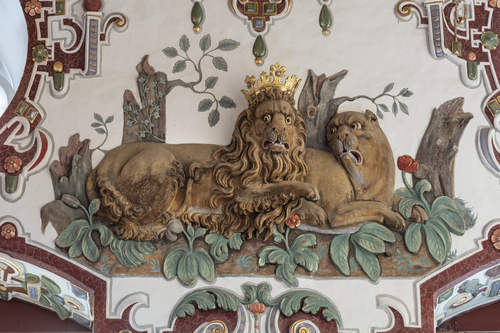
\includegraphics{paintings_files/figure-pdf/cell-3-output-4.png}

Wikibase link:
\url{https://computational-publishing-service.wikibase.cloud/entity/Q214}

Title: Bär -- Gesamtansicht

Year: 2018

Description: Gerhardt Schmidt, Bildhauer - Mitarbeit: Christoph
Limmerich, Bildhauer - Mitarbeit: Caspar Dieterich, Fassmaler -
Weikersheim, Schloss Weikersheim, Rittersaal \& Raum 72 - Vollendung:
1605 - 1747

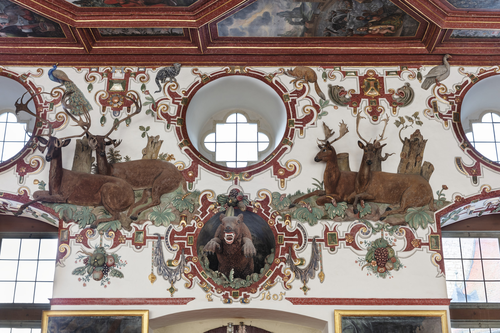
\includegraphics{paintings_files/figure-pdf/cell-3-output-6.png}

Wikibase link:
\url{https://computational-publishing-service.wikibase.cloud/entity/Q215}

Title: Hirschpaare -- Gesamtansicht

Year: 2018

Description: Gerhardt Schmidt, Bildhauer - Mitarbeit: Christoph
Limmerich, Bildhauer - Mitarbeit: Caspar Dieterich, Fassmaler -
Weikersheim, Schloss Weikersheim, Rittersaal \& Raum 72 - Vollendung:
1605 - 1747

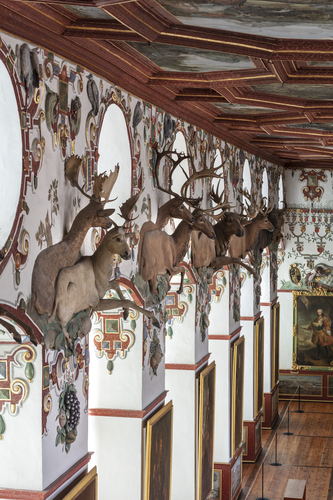
\includegraphics{paintings_files/figure-pdf/cell-3-output-8.png}

Wikibase link:
\url{https://computational-publishing-service.wikibase.cloud/entity/Q216}

Title: Affe -- Gesamtansicht

Year: 2018

Description: Gerhardt Schmidt, Bildhauer - Mitarbeit: Christoph
Limmerich, Bildhauer - Mitarbeit: Caspar Dieterich, Fassmaler -
Weikersheim, Schloss Weikersheim, Rittersaal \& Raum 72 - Vollendung:
1605 - 1747

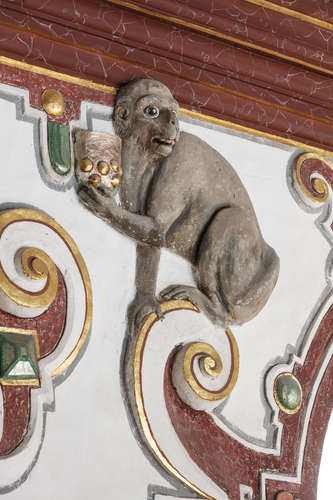
\includegraphics{paintings_files/figure-pdf/cell-3-output-10.png}

Wikibase link:
\url{https://computational-publishing-service.wikibase.cloud/entity/Q220}

Title: Saalbau -- Gartenseite des Schlosses von Süden

Year: 2021

Description: Wolfgang Beringer, Baumeister \& Steinmetz - Georg Stegle,
Baumeister - Entwurf: Georges Robin, Architekt - Elias Gunzenhäuser,
Zimmermann - Weikersheim, Marktplatz 11 - ab 1595

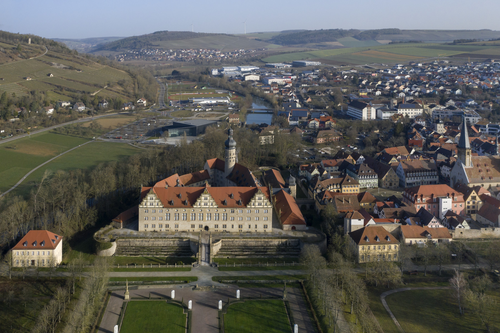
\includegraphics{paintings_files/figure-pdf/cell-3-output-12.png}

Wikibase link:
\url{https://computational-publishing-service.wikibase.cloud/entity/Q221}

Title: Saalbau -- von Südosten

Year: 2021

Description: Wolfgang Beringer, Baumeister \& Steinmetz - Georg Stegle,
Baumeister - Entwurf: Georges Robin, Architekt - Elias Gunzenhäuser,
Zimmermann - Weikersheim, Marktplatz 11 - ab 1595

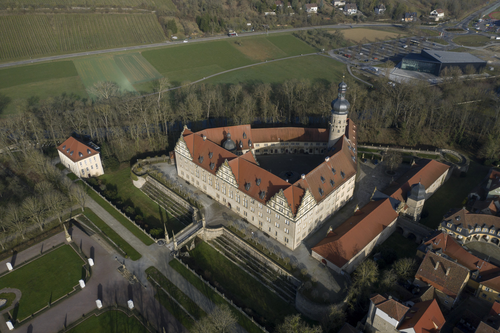
\includegraphics{paintings_files/figure-pdf/cell-3-output-14.png}

Wikibase link:
\url{https://computational-publishing-service.wikibase.cloud/entity/Q224}

Title: Erschließungsraumfolgen

Year: 2020

Description: text

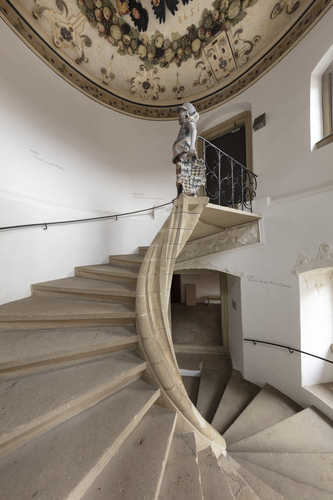
\includegraphics{paintings_files/figure-pdf/cell-3-output-16.png}

Wikibase link:
\url{https://computational-publishing-service.wikibase.cloud/entity/Q225}

Title: Deckendekoration des Treppenturms

Year: 2020

Description: Deckendekoration

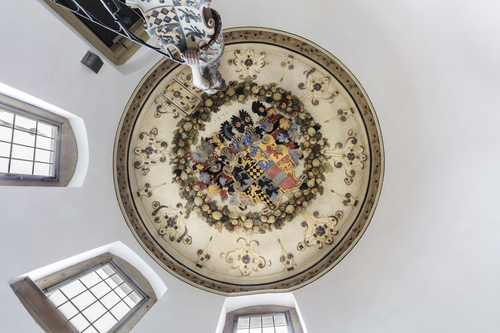
\includegraphics{paintings_files/figure-pdf/cell-3-output-18.png}

Wikibase link:
\url{https://computational-publishing-service.wikibase.cloud/entity/Q230}

Title: Deckendekoration des Rittersaals -- Östliche Partie der Decke

Year: 2018

Description: Balthasar Kazenberger, Maler, 22.09.1601/22.11.1602 - Jan
van der Straet, Maler - Christian Thalwitzer, Restaurator, 1710/1711

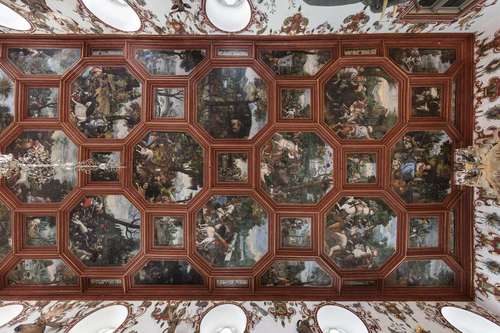
\includegraphics{paintings_files/figure-pdf/cell-3-output-20.png}

Wikibase link:
\url{https://computational-publishing-service.wikibase.cloud/entity/Q234}

Title: Einstige Tafelstube \& Raum 69a -- nach Südosten

Year: 2018

Description: Wolfgang Beringer, Baumeister und Steinmetz - Georg Stegle,
Baumeister - Entwurf: Georges Robin, Architekt - Elias Gunzenhäuser,
Zimmermann - Weikersheim, Marktplatz 11 - ab 1595

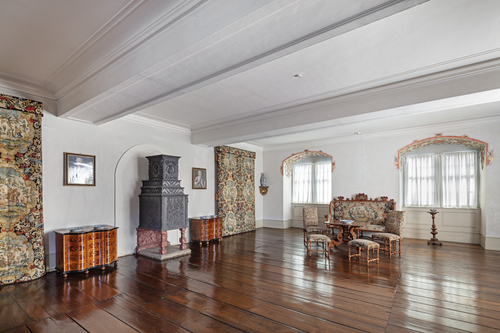
\includegraphics{paintings_files/figure-pdf/cell-3-output-22.png}

Wikibase link:
\url{https://computational-publishing-service.wikibase.cloud/entity/Q251}

Title: Der Saalbau Bild

Year: 2018

Description: Ein Bild vom Saalbau

\begin{verbatim}
UnidentifiedImageError: cannot identify image file <_io.BytesIO object at 0x786f22fa8400>
---------------------------------------------------------------------------
UnidentifiedImageError                    Traceback (most recent call last)
Cell In[3], line 1
----> 1 get_img()

Cell In[2], line 141, in get_img()
    139 image_url=item['imgUrl']['value']
    140 headers = {'User-Agent': 'Ex_Books_conference_bot/0.0 (https://github.com/SimonXIX/Experimental_Books_workshop; ad7588@coventry.ac.uk)'}
--> 141 im = fetch_image_by_url(image_url, headers)
    142 im.thumbnail((500, 500), Image.Resampling.LANCZOS)
    143 display(im)

Cell In[2], line 117, in fetch_image_by_url(url, headers)
    115 r = requests.get(url, headers=headers, stream=True)
    116 if r.status_code == 200:
--> 117     im = Image.open(r.raw)
    118     return im
    119 if r.status_code == 500:

File ~/.local/lib/python3.10/site-packages/PIL/Image.py:3498, in open(fp, mode, formats)
   3496     warnings.warn(message)
   3497 msg = "cannot identify image file %r" % (filename if filename else fp)
-> 3498 raise UnidentifiedImageError(msg)

UnidentifiedImageError: cannot identify image file <_io.BytesIO object at 0x786f22fa8400>
\end{verbatim}

\bookmarksetup{startatroot}

\chapter{Data Visualisation}\label{data-visualisation}

Generate wordcloud

\begin{verbatim}
C:\Users\worthingtons\AppData\Local\Packages\PythonSoftwareFoundation.Python.3.11_qbz5n2kfra8p0\LocalCache\local-packages\Python311\site-packages\VizKG\utils\util.py:89: UserWarning: Could not infer format, so each element will be parsed individually, falling back to `dateutil`. To ensure parsing is consistent and as-expected, please specify a format.
  dataframe[column] = dataframe[column].astype('datetime64')
C:\Users\worthingtons\AppData\Local\Packages\PythonSoftwareFoundation.Python.3.11_qbz5n2kfra8p0\LocalCache\local-packages\Python311\site-packages\VizKG\utils\util.py:89: UserWarning: Could not infer format, so each element will be parsed individually, falling back to `dateutil`. To ensure parsing is consistent and as-expected, please specify a format.
  dataframe[column] = dataframe[column].astype('datetime64')
\end{verbatim}

\includegraphics{datavis_files/figure-pdf/cell-3-output-2.png}

\bookmarksetup{startatroot}

\chapter{Der Große Saal
(Rittersaal)}\label{der-grouxdfe-saal-rittersaal}

\textbf{How to use your own text for processing}

\begin{enumerate}
\def\labelenumi{\arabic{enumi}.}
\tightlist
\item
  Add a new Text item to the wikibase.
  \href{https://computational-publishing-service.wikibase.cloud/wiki/Special:NewItem}{link
  to wikibase new item} the item should contain the following
  statements:
\end{enumerate}

\begin{itemize}
\tightlist
\item
  P57 (external link): link to the html file containing the new text
\item
  P46 (kurator): Item of the curator. you may use an existing item like
  Q210 (Ulrike seeger) for test purposes
\item
  P53 (license): Item of a license for the text. e.g Q203 (CC BY-NC-ND
  4.0 DEED )
\item
  P6 (is part of): set value to Q218 (Schlossanlage Weikersheim)
\end{itemize}

\begin{enumerate}
\def\labelenumi{\arabic{enumi}.}
\setcounter{enumi}{1}
\item
  check if your new text item occurs in the list of selected text items:
  \href{https://computational-publishing-service.wikibase.cloud/query/\#PREFIX\%20cps\%3A\%20\%3Chttps\%3A\%2F\%2Fcomputational-publishing-service.wikibase.cloud\%2Fentity\%2F\%3E\%0APREFIX\%20cpss\%3A\%20\%3Chttps\%3A\%2F\%2Fcomputational-publishing-service.wikibase.cloud\%2Fentity\%2Fstatement\%2F\%3E\%0APREFIX\%20cpsv\%3A\%20\%3Chttps\%3A\%2F\%2Fcomputational-publishing-service.wikibase.cloud\%2Fvalue\%2F\%3E\%0APREFIX\%20cpspt\%3A\%20\%3Chttps\%3A\%2F\%2Fcomputational-publishing-service.wikibase.cloud\%2Fprop\%2Fdirect\%2F\%3E\%0APREFIX\%20cpsp\%3A\%20\%3Chttps\%3A\%2F\%2Fcomputational-publishing-service.wikibase.cloud\%2Fprop\%2F\%3E\%0APREFIX\%20cpsps\%3A\%20\%3Chttps\%3A\%2F\%2Fcomputational-publishing-service.wikibase.cloud\%2Fprop\%2Fstatement\%2F\%3E\%0APREFIX\%20cpspq\%3A\%20\%3Chttps\%3A\%2F\%2Fcomputational-publishing-service.wikibase.cloud\%2Fprop\%2Fqualifier\%2F\%3E\%0A\%0ASELECT\%20\%3FtextItem\%20\%3FkuratorLabel\%20\%3FtextUrl\%0AWHERE\%0A\%7B\%0A\%20\%20\%3FtextItem\%20cpsp\%3AP46\%20\%3FkuratorStatement.\%20\%0A\%20\%20\%3FkuratorStatement\%20cpsps\%3AP46\%20\%3FkuratorItem.\%20\%0A\%20\%20\%3FkuratorItem\%20rdfs\%3Alabel\%20\%3FkuratorLabel.\%0A\%20\%20\%3FtextItem\%20cpsp\%3AP57\%20\%3Furlstatement.\%20\%0A\%20\%20\%3Furlstatement\%20cpsps\%3AP57\%20\%3FtextUrl.\%20\%0A\%7D}{Link
  to wikibase query service}
\item
  set parameter of get\_text() to the id of your new text item e.g.:
  get\_text(``Q209'')
\end{enumerate}

Wikibase link:
\url{https://computational-publishing-service.wikibase.cloud/entity/Q219}

Kurator: Seeger, Ulrike

\bookmarksetup{startatroot}

\chapter{Schlossanlage Weikersheim}\label{schlossanlage-weikersheim}

Lorem ipsum dolor sit amet, consectetur adipiscing elit. Integer ut
vehicula purus, vitae viverra ante. Vivamus faucibus sem ac libero
blandit, ut auctor risus porta. Cras non dapibus magna. Curabitur
dignissim est sed porttitor pretium. Fusce ex nunc, dignissim non
bibendum vitae, ultrices non nisl. Sed eget tincidunt enim. Duis
eleifend sapien ac lectus vestibulum rhoncus.

\textbf{How to select images for processing}

Images are selected via the sparql query. The method get\_img() is
capable of using a wikibase item id as parameter to select images with
the property P6 (is part of) linking to the given item id.

\begin{enumerate}
\def\labelenumi{\arabic{enumi}.}
\item
  select a valid location id from the query result:
  \href{https://computational-publishing-service.wikibase.cloud/query/\#PREFIX\%20cps\%3A\%20\%3Chttps\%3A\%2F\%2Fcomputational-publishing-service.wikibase.cloud\%2Fentity\%2F\%3E\%0APREFIX\%20cpss\%3A\%20\%3Chttps\%3A\%2F\%2Fcomputational-publishing-service.wikibase.cloud\%2Fentity\%2Fstatement\%2F\%3E\%0APREFIX\%20cpsv\%3A\%20\%3Chttps\%3A\%2F\%2Fcomputational-publishing-service.wikibase.cloud\%2Fvalue\%2F\%3E\%0APREFIX\%20cpspt\%3A\%20\%3Chttps\%3A\%2F\%2Fcomputational-publishing-service.wikibase.cloud\%2Fprop\%2Fdirect\%2F\%3E\%0APREFIX\%20cpsp\%3A\%20\%3Chttps\%3A\%2F\%2Fcomputational-publishing-service.wikibase.cloud\%2Fprop\%2F\%3E\%0APREFIX\%20cpsps\%3A\%20\%3Chttps\%3A\%2F\%2Fcomputational-publishing-service.wikibase.cloud\%2Fprop\%2Fstatement\%2F\%3E\%0APREFIX\%20cpspq\%3A\%20\%3Chttps\%3A\%2F\%2Fcomputational-publishing-service.wikibase.cloud\%2Fprop\%2Fqualifier\%2F\%3E\%0A\%0ASELECT\%20DISTINCT\%20\%3FpartOfItem\%20\%3FpartOfItemLabel\%0AWHERE\%0A\%7B\%0A\%20\%20\%3FimgItem\%20cpsp\%3AP107\%20\%3FurlStatement.\%20\%0A\%20\%20\%3FurlStatement\%20cpsps\%3AP107\%20\%3FimgUrl.\%20\%0A\%20\%20\%3FimgItem\%20cpsp\%3AP60\%20\%3FdateStatement.\%20\%0A\%20\%20\%3FdateStatement\%20cpsps\%3AP60\%20\%3FpublishDate.\%20\%0A\%20\%20\%3FimgItem\%20cpsp\%3AP6\%20\%3FpartOfStatement.\%0A\%20\%20\%3FpartOfStatement\%20cpsps\%3AP6\%20\%3FpartOfItem.\%0A\%20\%20SERVICE\%20wikibase\%3Alabel\%20\%7B\%0A\%20\%20\%20\%20\%20\%20bd\%3AserviceParam\%20wikibase\%3Alanguage\%20\%22de\%2Cen\%22.\%0A\%20\%20\%20\%20\%20\%20\%3FpartOfItem\%20rdfs\%3Alabel\%20\%3FpartOfItemLabel.\%0A\%20\%20\%20\%20\%20\%20\%3FpartOfItem\%20schema\%3Adescription\%20\%3FpartOfItemDescr.\%0A\%20\%20\%20\%20\%7D\%0A\%7D\%20GROUP\%20BY\%20\%3FpartOfItem\%20\%3FpartOfItemLabel}{Link
  to wikibase query service}
\item
  set parameter of get\_img() to the id of your selected location item
  e.g.: get\_img(``Q217'')
\end{enumerate}

Wikibase link:
\url{https://computational-publishing-service.wikibase.cloud/entity/Q212}

Title: Knight's Hall \& Room 72 - to the west

Year: 2018

Description: Part of: Weikersheim Castle Saalbau Wolfgang Beringer,
builder \& Stonemason - Georg Stegle, master builder - design: Georges
Robin, architect - Elias Gunzenhäuser, carpenter - Weikersheim,
Marktplatz 11 - from 1595

\begin{figure}[H]

{\centering 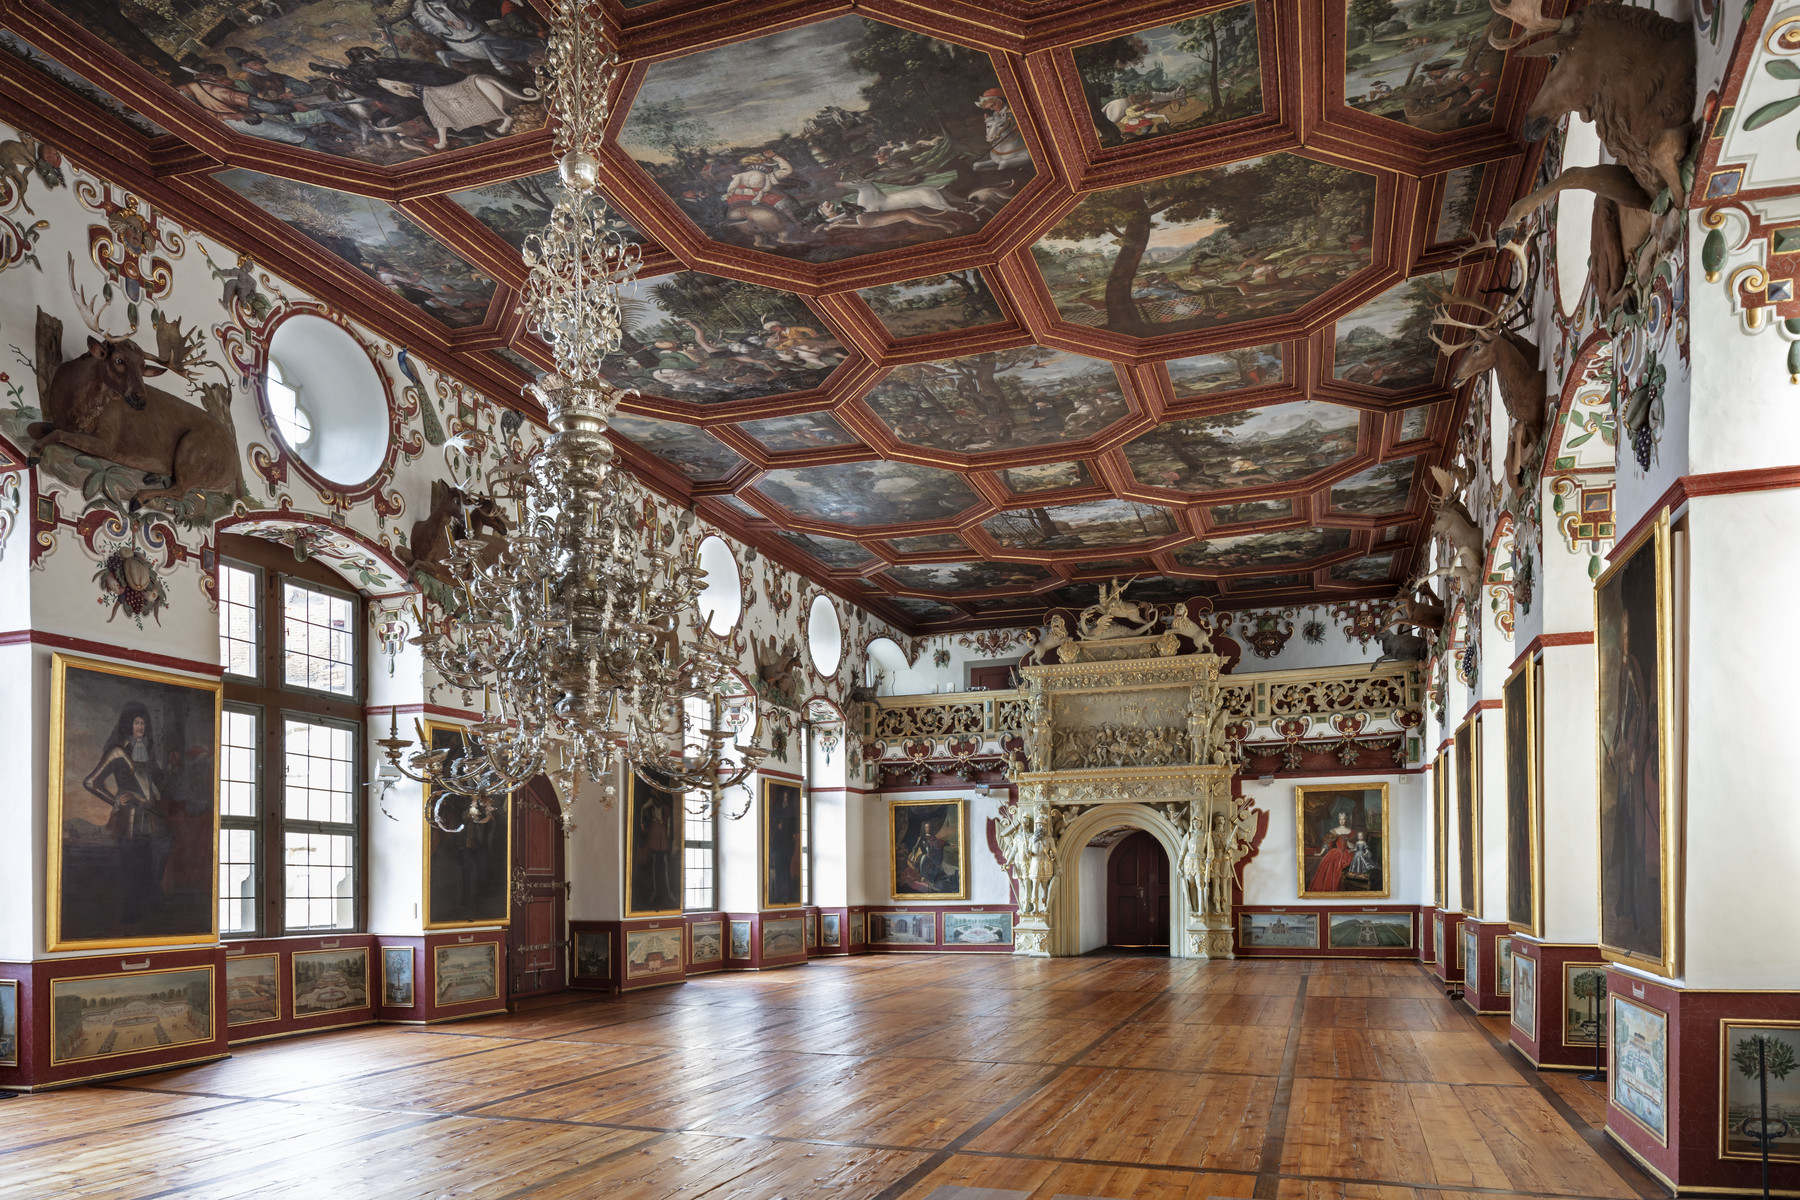
\includegraphics{impressum_files/mediabag/fmd10005862a.jpg}

}

\caption{Knight's Hall \& Room 72 - to the west}

\end{figure}%

Wikibase link:
\url{https://computational-publishing-service.wikibase.cloud/entity/Q213}

Title: Lion couple -- general view

Year: 2018

Description: Gerhardt Schmidt, sculptor - collaboration: Christoph
Limmerich, sculptor - collaboration: Caspar Dieterich, barrel painter -
Weikersheim, Weikersheim Castle, Knight's Hall \& Room 72 - Completion:
1605 - 1747

\begin{figure}[H]

{\centering 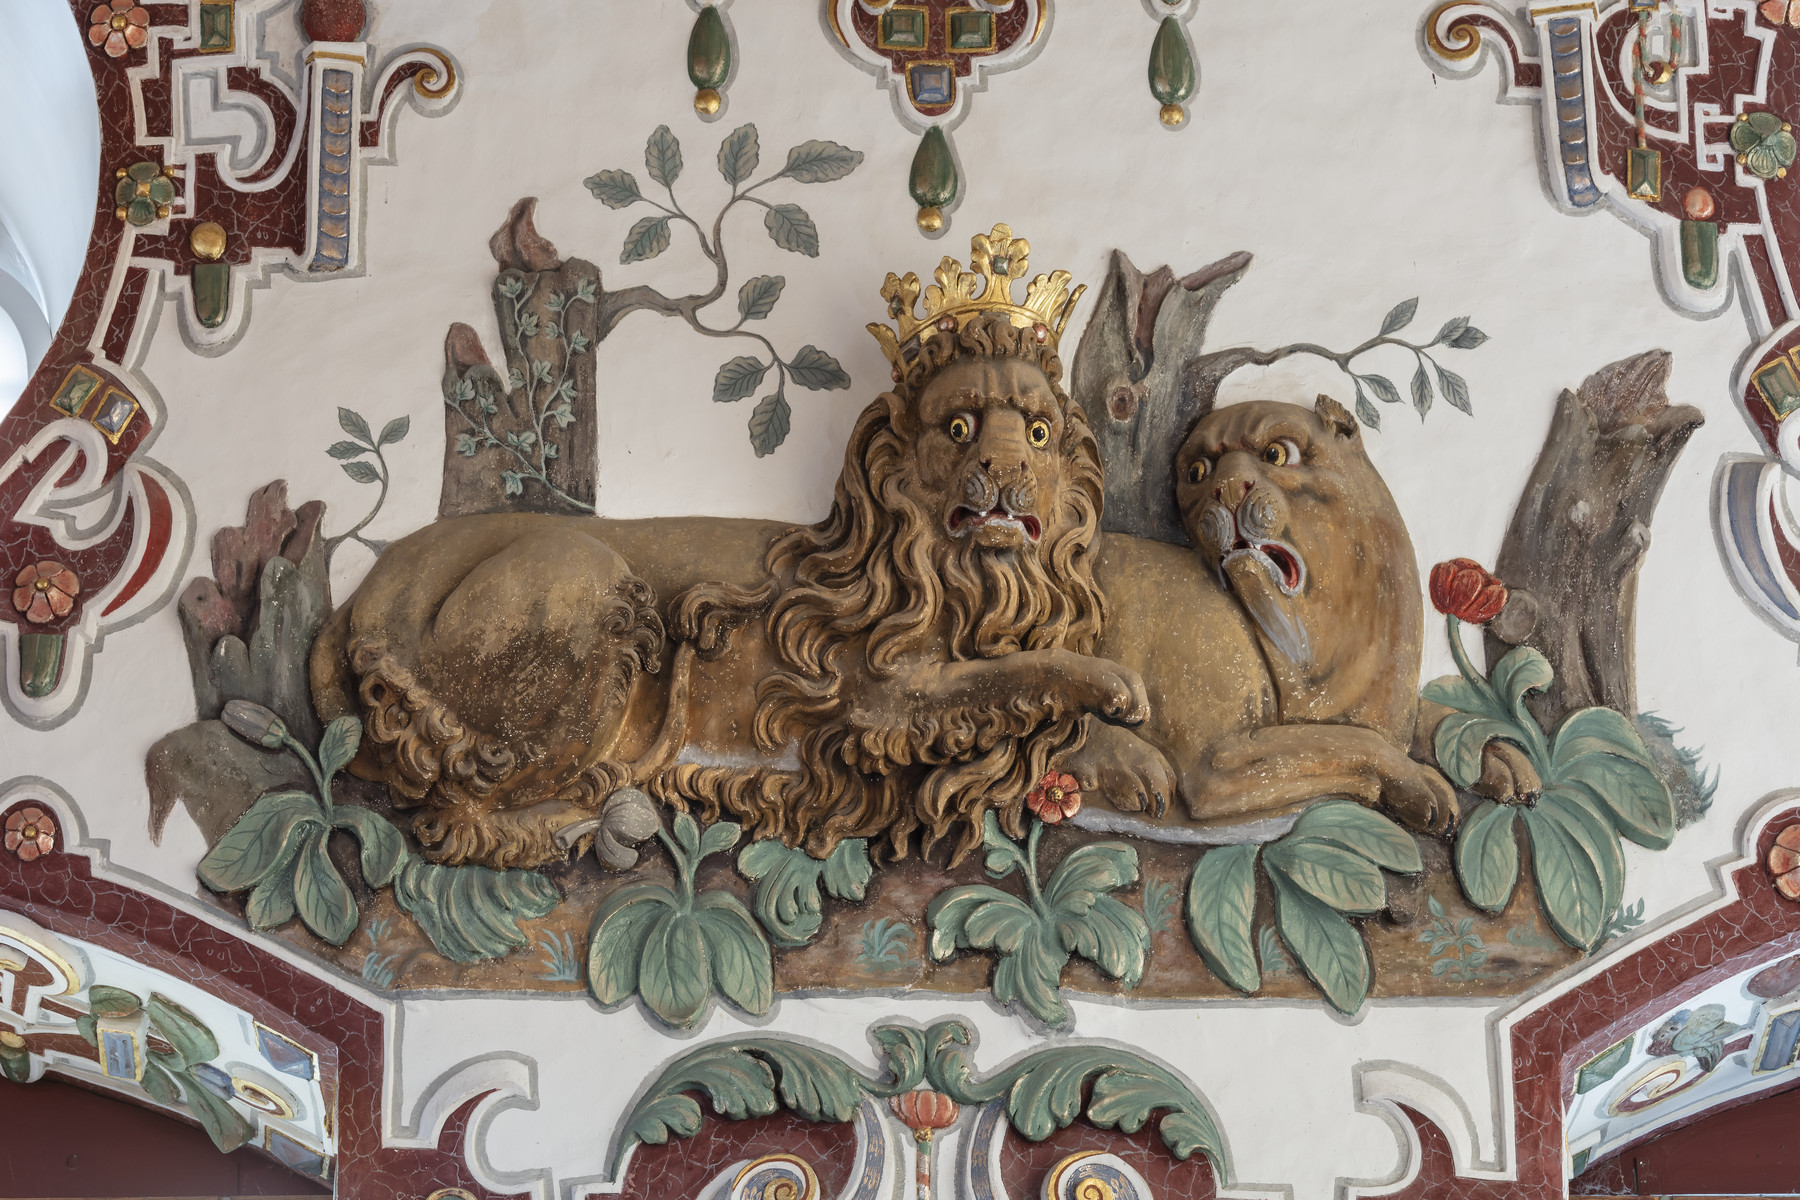
\includegraphics{impressum_files/mediabag/fmd10005864a.jpg}

}

\caption{Lion couple -- general view}

\end{figure}%

Wikibase link:
\url{https://computational-publishing-service.wikibase.cloud/entity/Q214}

Title: Bear -- general view

Year: 2018

Description: Gerhardt Schmidt, sculptor - collaboration: Christoph
Limmerich, sculptor - collaboration: Caspar Dieterich, barrel painter -
Weikersheim, Weikersheim Castle, Knight's Hall \& Room 72 - Completion:
1605 - 1747

\begin{figure}[H]

{\centering 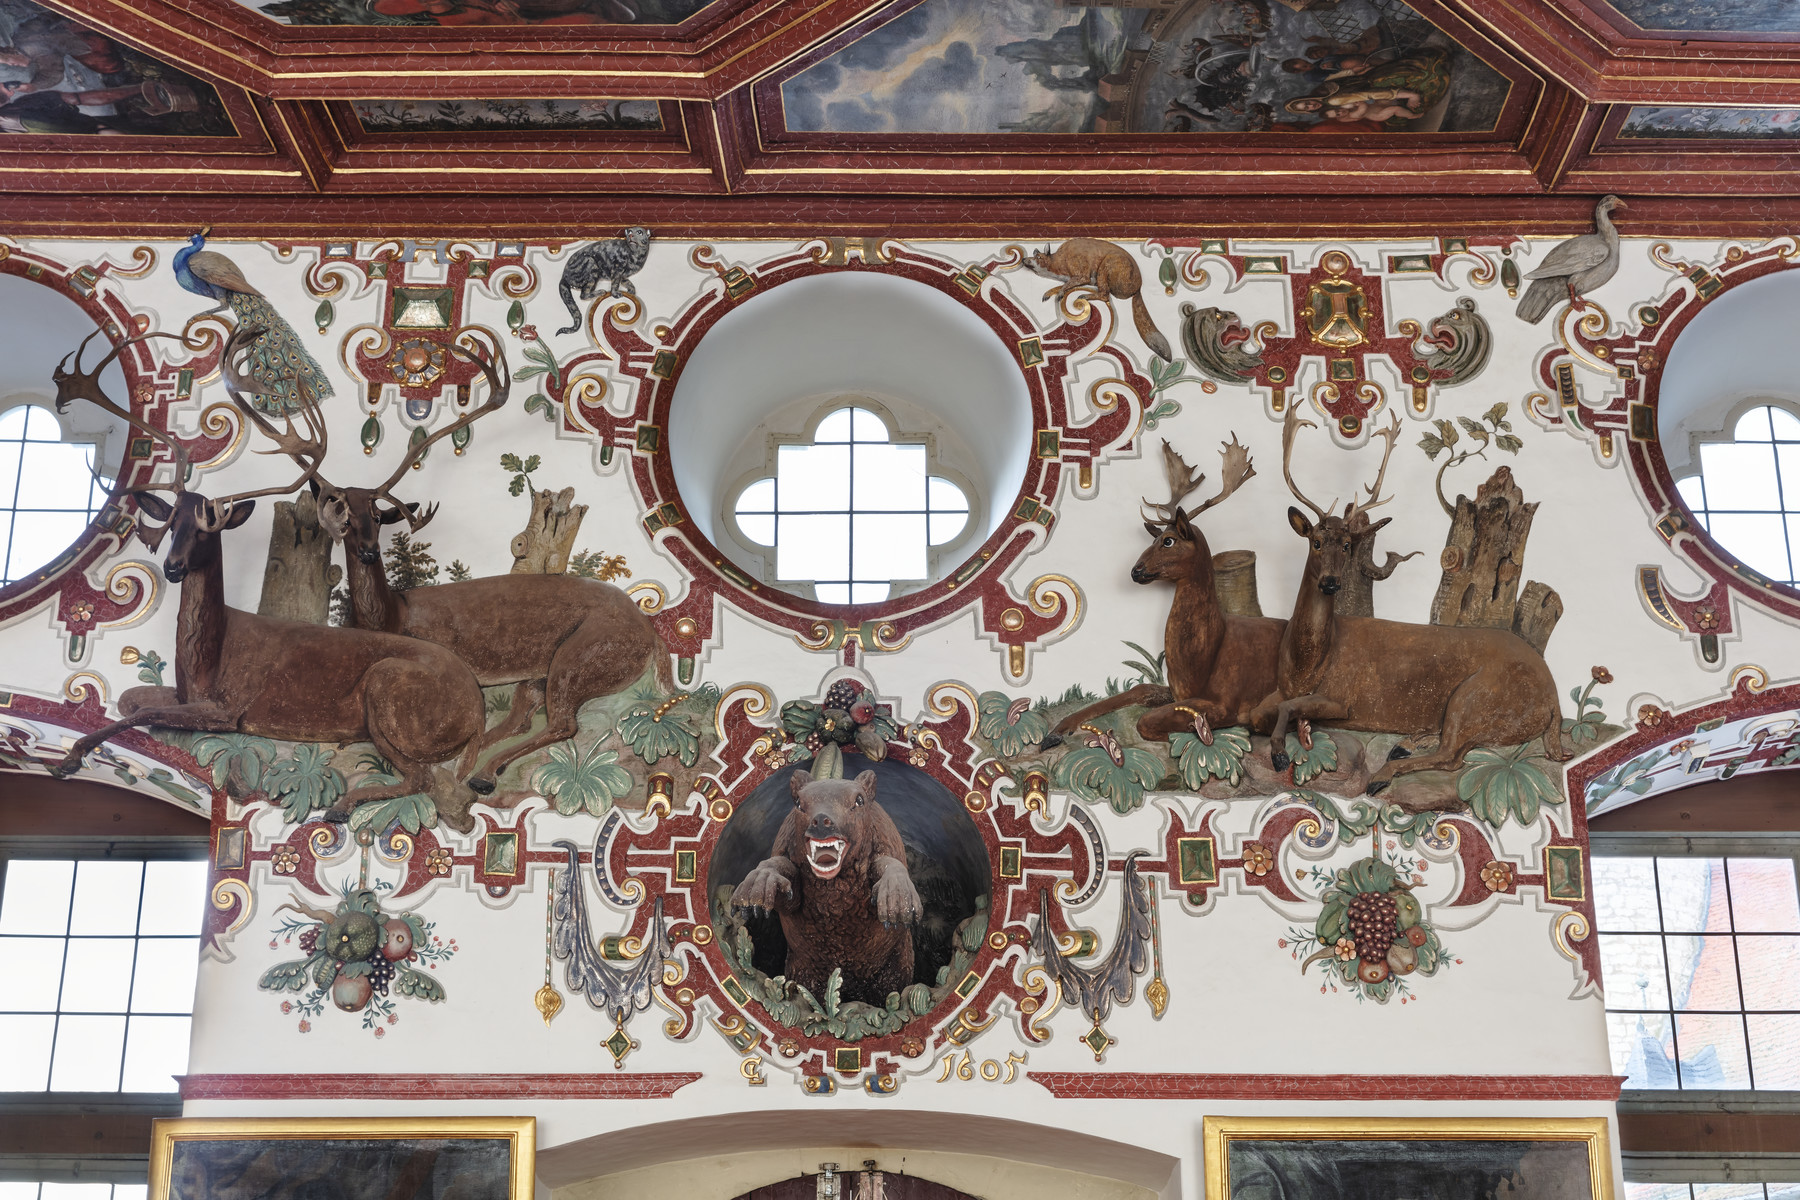
\includegraphics{impressum_files/mediabag/fmd10005865a.jpg}

}

\caption{Bear -- general view}

\end{figure}%

Wikibase link:
\url{https://computational-publishing-service.wikibase.cloud/entity/Q216}

Title: Monkey -- general view

Year: 2018

Description: Gerhardt Schmidt, sculptor - collaboration: Christoph
Limmerich, sculptor - collaboration: Caspar Dieterich, barrel painter -
Weikersheim, Weikersheim Castle, Knight's Hall \& Room 72 - Completion:
1605 - 1747

\begin{figure}[H]

{\centering 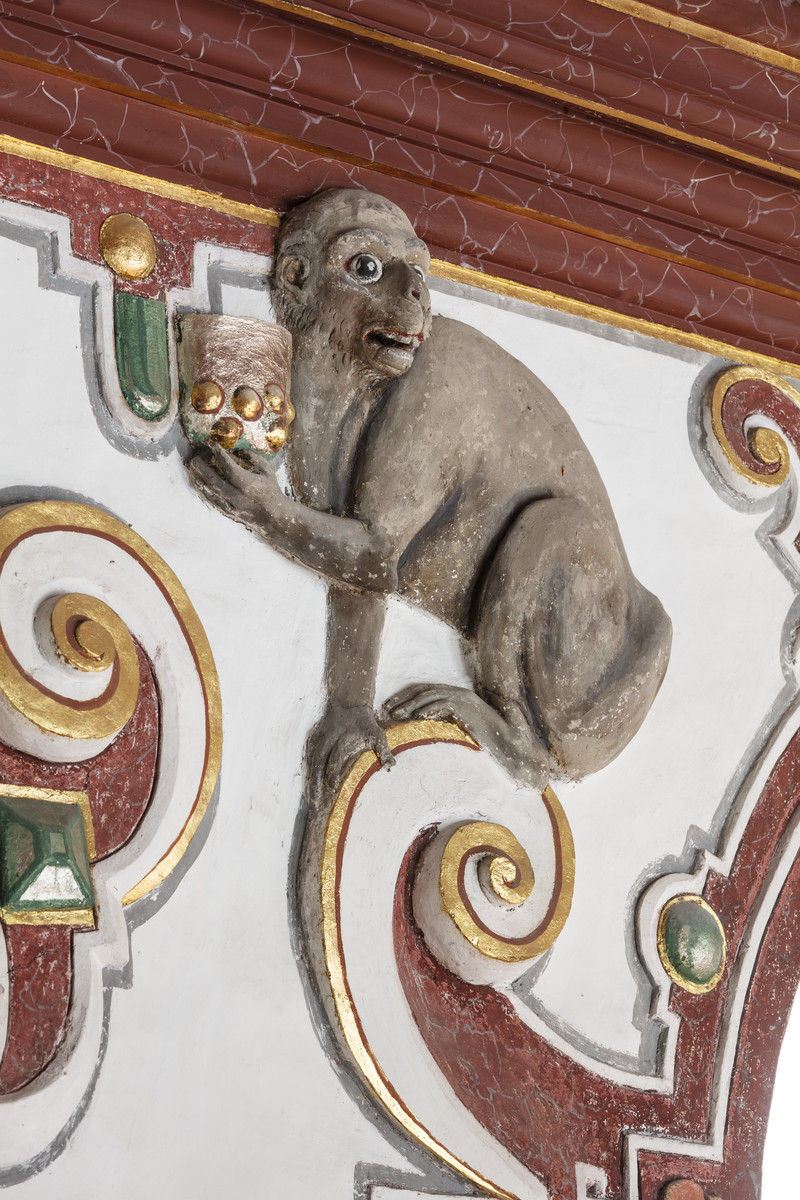
\includegraphics{impressum_files/mediabag/fmd10005867a.jpg}

}

\caption{Monkey -- general view}

\end{figure}%

Wikibase link:
\url{https://computational-publishing-service.wikibase.cloud/entity/Q215}

Title: Deer pairs -- general view

Year: 2018

Description: Gerhardt Schmidt, sculptor - collaboration: Christoph
Limmerich, sculptor - collaboration: Caspar Dieterich, barrel painter -
Weikersheim, Weikersheim Castle, Knight's Hall \& Room 72 - Completion:
1605 - 1747

\begin{figure}[H]

{\centering 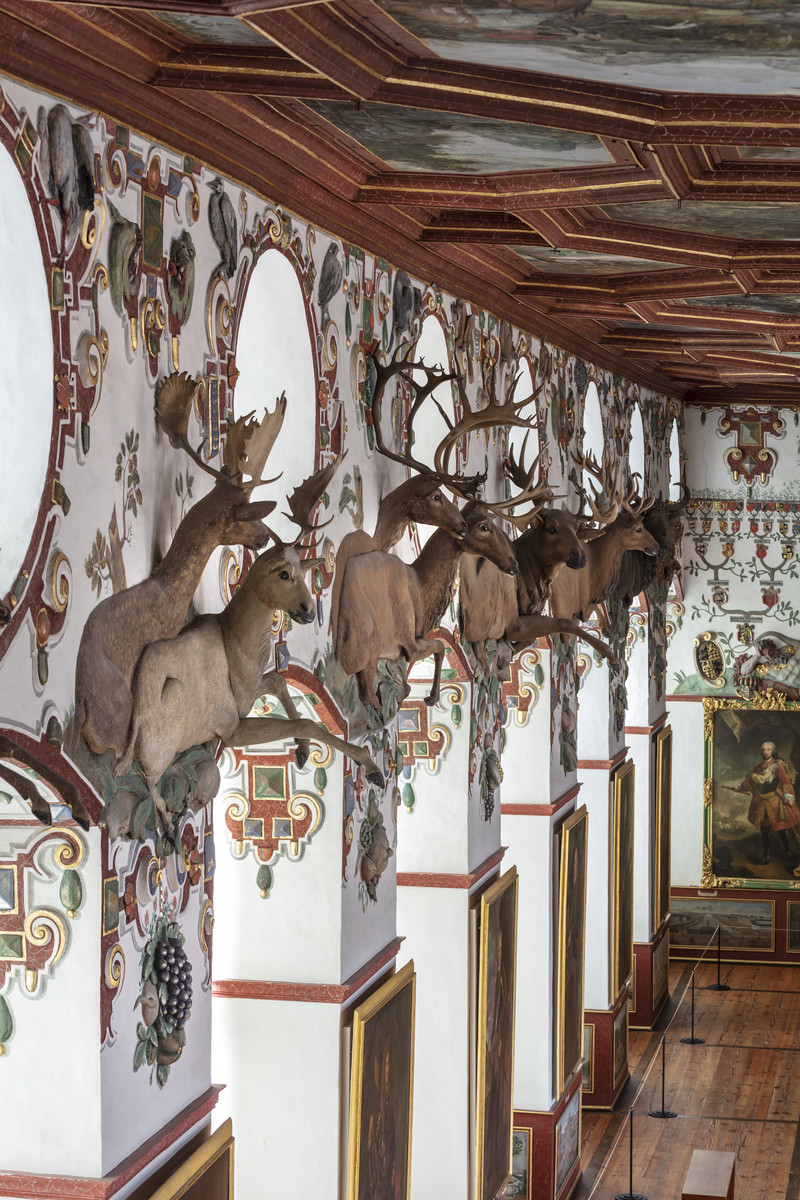
\includegraphics{impressum_files/mediabag/fmd10005866a.jpg}

}

\caption{Deer pairs -- general view}

\end{figure}%

Wikibase link:
\url{https://computational-publishing-service.wikibase.cloud/entity/Q200}

Title: Knight's Hall \& Room 72 - to the east

Year: 2018

Description: Part of: Weikersheim Castle SaalbauWolfgang Beringer,
builder \& Stonemason - Georg Stegle, master builder - design: Georges
Robin, architect - Elias Gunzenhäuser, carpenter - Weikersheim,
Marktplatz 11 - from 1595

\begin{figure}[H]

{\centering 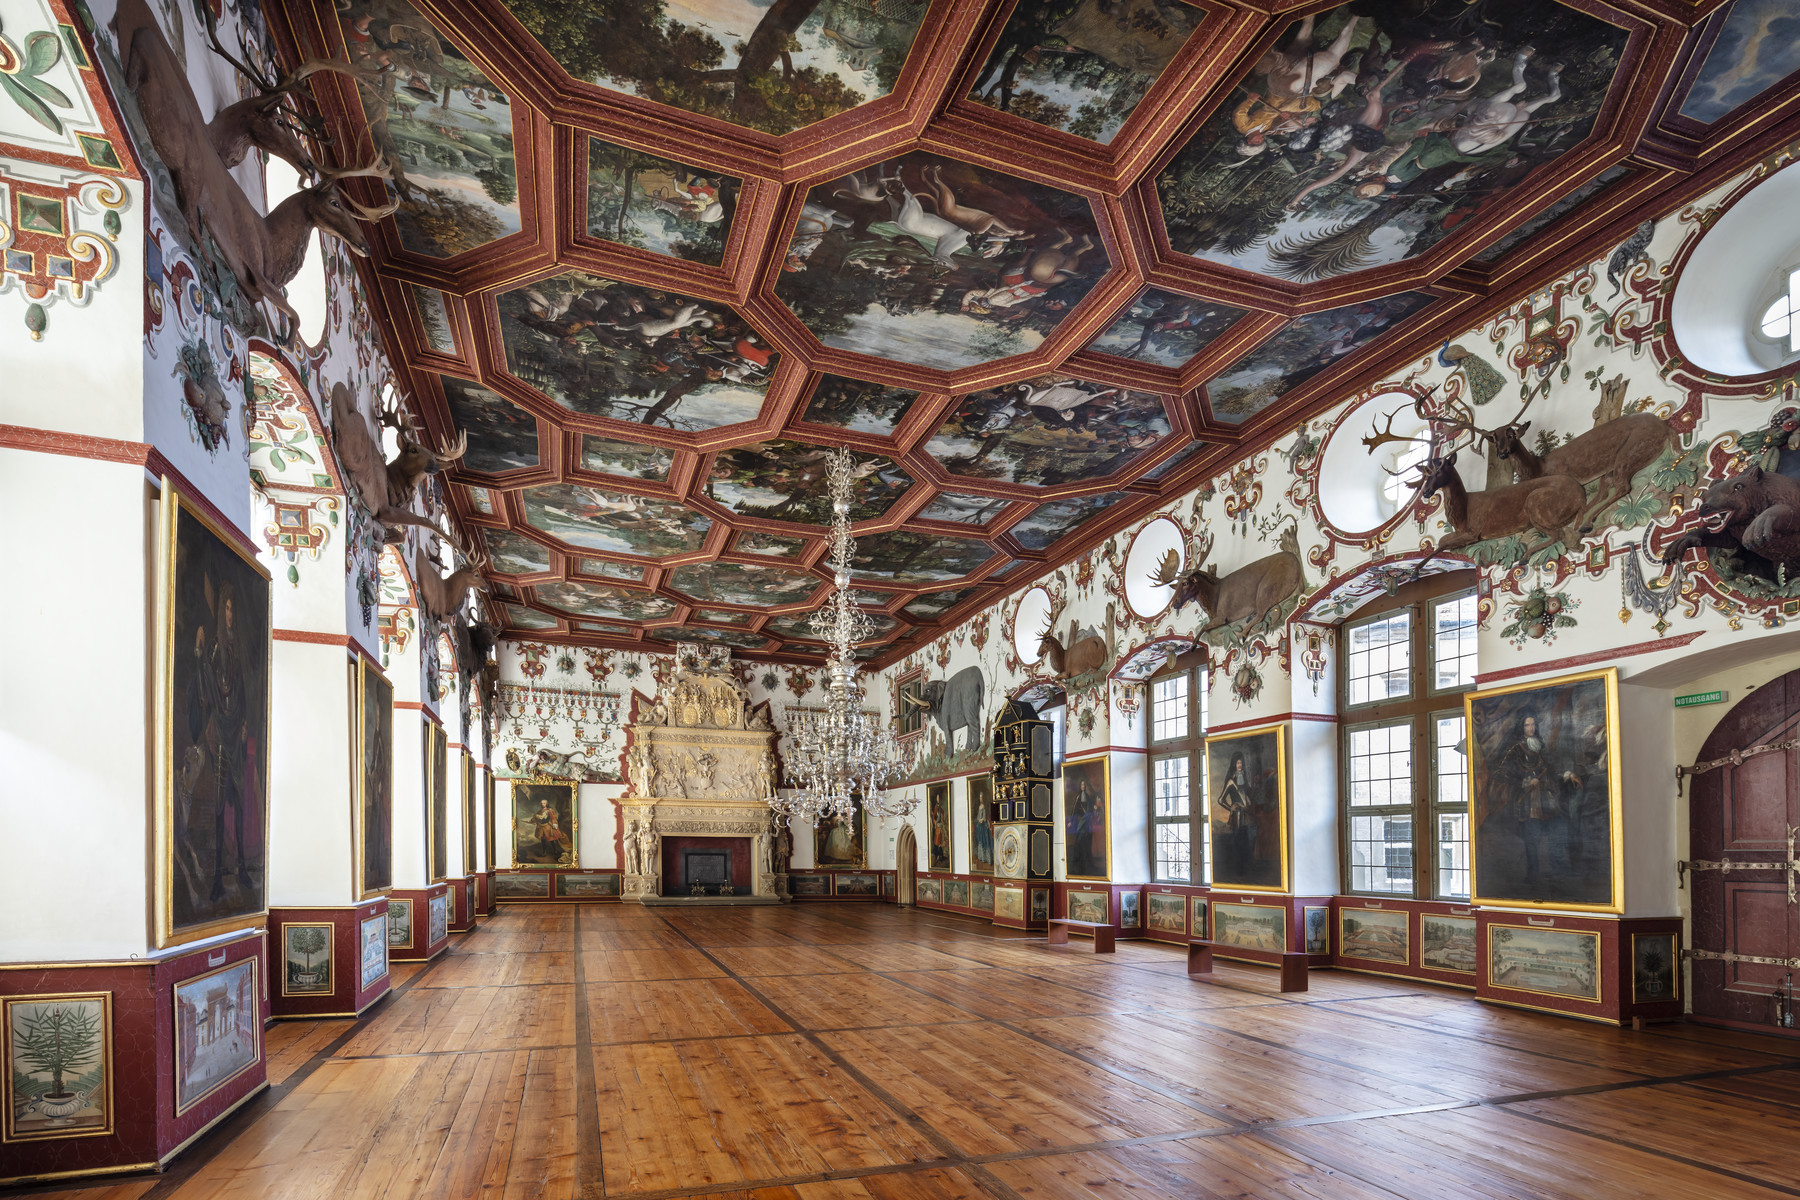
\includegraphics{impressum_files/mediabag/fmd10005859a.jpg}

}

\caption{Knight's Hall \& Room 72 - to the east}

\end{figure}%

Wikibase link:
\url{https://computational-publishing-service.wikibase.cloud/entity/Q211}

Title: Knight's Hall \& Room 72 - to the east

Year: 2018

Description: Part of: Weikersheim Castle Saalbau Wolfgang Beringer,
builder \& Stonemason - Georg Stegle, master builder - design: Georges
Robin, architect - Elias Gunzenhäuser, carpenter - Weikersheim,
Marktplatz 11 - from 1595

\begin{figure}[H]

{\centering 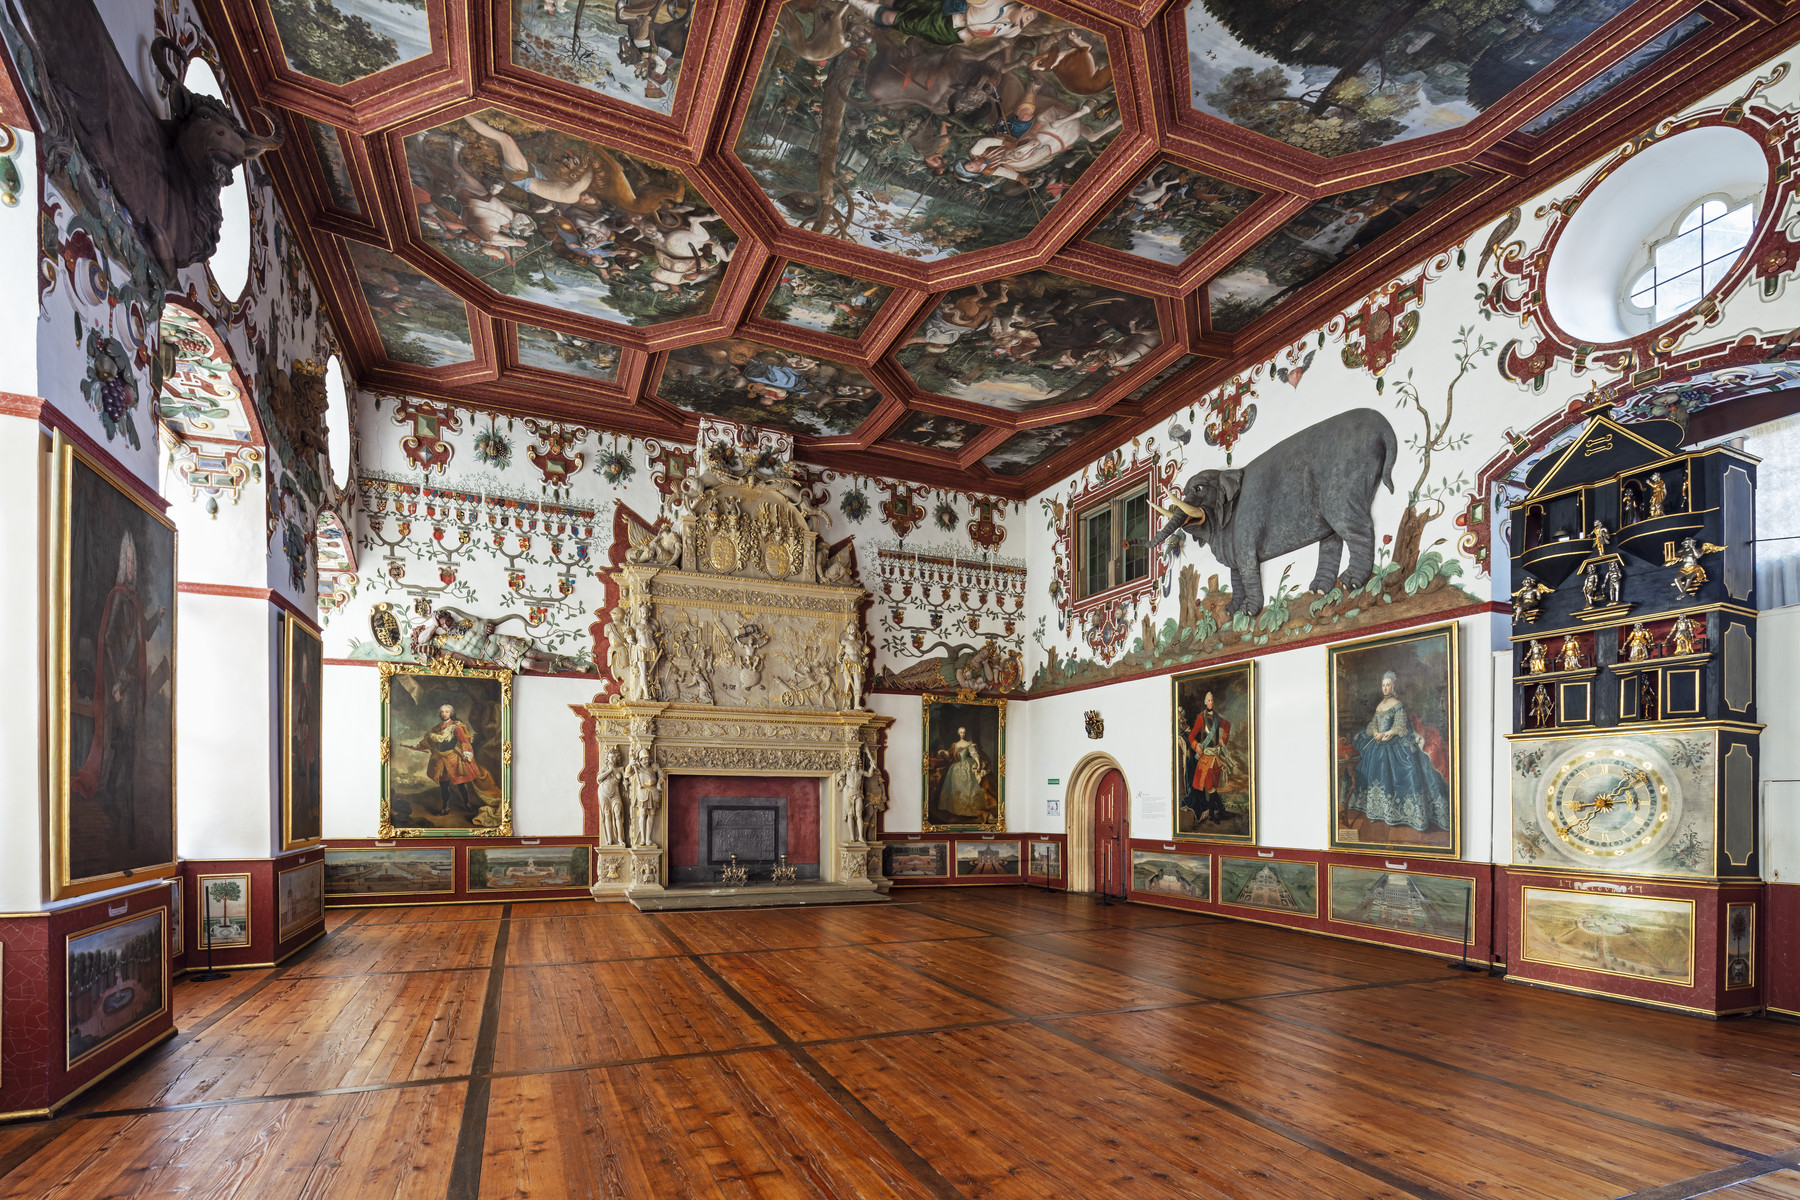
\includegraphics{impressum_files/mediabag/fmd10005860a.jpg}

}

\caption{Knight's Hall \& Room 72 - to the east}

\end{figure}%

\begin{verbatim}
C:\Users\worthingtons\AppData\Local\Packages\PythonSoftwareFoundation.Python.3.11_qbz5n2kfra8p0\LocalCache\local-packages\Python311\site-packages\VizKG\utils\util.py:89: UserWarning: Could not infer format, so each element will be parsed individually, falling back to `dateutil`. To ensure parsing is consistent and as-expected, please specify a format.
  dataframe[column] = dataframe[column].astype('datetime64')
C:\Users\worthingtons\AppData\Local\Packages\PythonSoftwareFoundation.Python.3.11_qbz5n2kfra8p0\LocalCache\local-packages\Python311\site-packages\VizKG\utils\util.py:89: UserWarning: Could not infer format, so each element will be parsed individually, falling back to `dateutil`. To ensure parsing is consistent and as-expected, please specify a format.
  dataframe[column] = dataframe[column].astype('datetime64')
\end{verbatim}

\includegraphics{rittersaal_files/figure-pdf/cell-5-output-2.png}

\bookmarksetup{startatroot}

\chapter{Gemälde-Sammlung: Wikidata
benchmark}\label{gemuxe4lde-sammlung-wikidata-benchmark}

Objective: Make a selection of nine paintings for the exhibition
catalogue to be selected from Wikidata and rendered multi-format in
Quarto.

The below Python code uses SPARQLWrapper to retrieve data from Wikidata
based on a SPARQL query.

This page acts as a `benchmark' to test if data fields can be read from
Wikidata.

Wikidata link: \url{http://www.wikidata.org/entity/Q29474642}

Title: The Birth of Benjamin

Year: 1650

Creator: Francesco Furini

Copyright: public domain

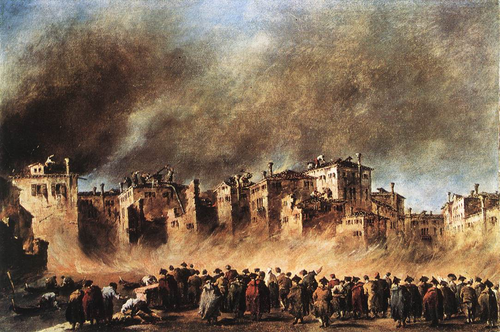
\includegraphics{painting-collection_files/figure-pdf/cell-2-output-2.png}

Wikidata link: \url{http://www.wikidata.org/entity/Q29474644}

Title: Venetian Gala Concert

Year: 1782

Creator: Francesco Guardi

Copyright: public domain

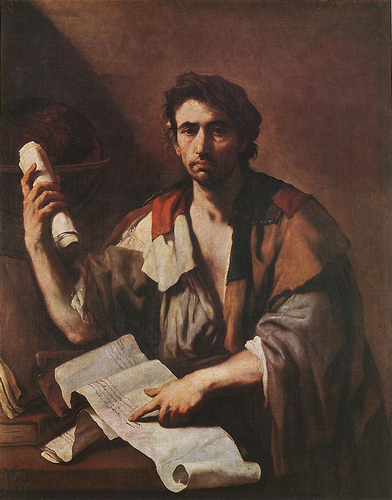
\includegraphics{painting-collection_files/figure-pdf/cell-2-output-4.png}

Wikidata link: \url{http://www.wikidata.org/entity/Q29474645}

Title: Q29474645

Year: 1789

Creator: Francesco Guardi

Copyright: public domain

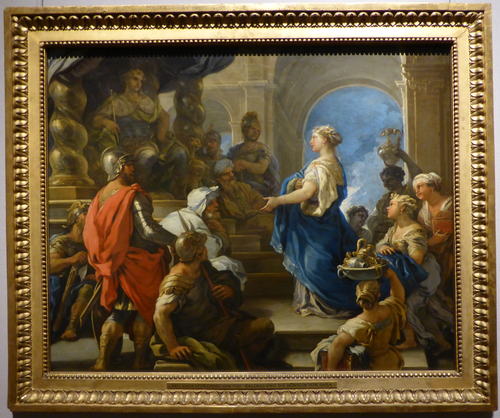
\includegraphics{painting-collection_files/figure-pdf/cell-2-output-6.png}


\backmatter


\end{document}
